% draft 3rd year diploma thesis, by Nick Manini, 2013/03/22
\documentclass[a4paper,12pt]{article}
\usepackage[english]{babel} % or other languages, e.g:
%\usepackage[italian]{babel} % needs debian package texlive-lang-italian
%\usepackage[latin1]{inputenc} % use to reproduce accented characters correctly
\usepackage{hyperref}
\usepackage{graphicx}
\usepackage{amsmath}
\usepackage{amssymb}
\usepackage{physics}
\usepackage{enumitem}
\usepackage{framed}
\usepackage[width=125mm]{caption}
\usepackage{lscape}
\usepackage[title,titletoc,toc]{appendix}

\graphicspath{{./media/images/}}

\usepackage[document]{ragged2e}
\usepackage{verbatim}
\usepackage{listings}
\usepackage{caption}
\usepackage{booktabs}

\usepackage{fixltx2e}

\usepackage{fancyhdr}
\pagestyle{fancy}
\fancyhead[LE,RO]{\slshape}
\fancyfoot[C]{\thepage}

%include the git footer with the last commit
%\include{gitfooter}

% Dimensione della pagina
\setlength{\oddsidemargin}{.3in}  % Distance from the left edge -1 inch 
\setlength{\textwidth}{145mm}     % Normal width of the text
\setlength{\topmargin}{.25in}     % Distance from top to PAGE'S HEAD -1 inch
\setlength{\textheight}{225mm}    % Height of the body of page
\setlength{\headheight}{0mm}      % Height of a box containing the head
\setlength{\parskip}{0.5mm}         % Extra vertical space before a paragraph
\setlength{\parindent}{9mm}       % Width of the indentation 
\linespread{1.12}                 % Line spacing        
\renewcommand{\floatpagefraction}{.9}

\usepackage{xcolor}
\newcommand\mynotes[1]{\begin{flushright}

\textcolor{red}{TODO: #1}\end{flushright}}
\newcommand{\jsqrt}[2]{\bqty{ #1 #1 | #2 #2 }}
\newcommand{\ksqrt}[2]{\bqty{ #1 #2 | #2 #1 }}
\newcommand\mf[1]{\mathbf{#1}}
\newcommand\dens{\rho(\mathbf{r})}
\newcommand\densin{\rho^{in}(\mathbf{r})}
\newcommand\densout{\rho^{out}(\mathbf{r})}
\newcommand\rdens{\tilde{\rho}(\mathbf{G})}
\newcommand\erre{\mathbf{r}}
\newcommand\GI{\mathbf{G}}
\newcommand\QE{\textsc{Quantum} ESPRESSO }
\newcommand\numbands{n_{bands}}
\newcommand\numG{n_{G}}
\newcommand\numR{n_{R}}
\newcommand\bigO{\mathcal{O}}
\newcommand\CO{Co\textsubscript{3}O\textsubscript{4} } 
%nome del sistema CO3

\begin{document}

\title{\bf \Huge Tuning the computational architecture for Quantum Espresso ab initio calculation of nanostructures }


\author{Giorgio Ruffa\\
Dipartimento di Fisica, Universit\`a degli Studi di Milano,\\
Via Celoria 16, 20133 Milano, Italia
}
\date{April 28, 2016} % the exact date of graduation, when available


{
\thispagestyle{empty}

\centerline{

\includegraphics[width=120mm,angle=0,clip=]{UniversitasMediolanensis.eps}
}

\begin{center}
{\Large Facolt\`a di Scienze e Tecnologie\\
\vskip0.2cm Laurea Triennale in Fisica }
\end{center}


\vskip1.5cm
\begin{center}
{\huge \textbf{Titolazzo della tesi, if seems long\\go to newline}}
\end{center}

{\large
\vskip20mm Relatore:  Prof. Dario Tamascelli
\vskip 1mm Correlatore: Prof. Michele Ceotto\\
\vskip 1mm Relatore Esterno: Dott. Davide Ceresoli\\
}

\vskip2cm
\hskip9cm\parbox[t]{7cm}
{\large 
Giorgio Ruffa\\
Matricola n$^\circ$ $742031$\\
A.A. $2015$/$2016$\\
\vskip 0.5mm Codice PACS: ?9.?a.?Z
}

\newpage
\newpage
\thispagestyle{empty}
\clearpage
}

 % eccezionalmente qui include il frontespizio
% in general avoid \include altoghether, it is looking for trouble !!

\newpage\qquad
\newpage

\maketitle

%---------------------------------------------------------
\begin{abstract}

Quantum Espresso (QE) is one of the most reliable and widespread  suite of codes for quantum chemistry calculations of nanostructures. Given the relevance of QE for the condensed matter physics community, we perform a detailed analysis of the information flow within the QE codes. We undertake several nanostructure systems to highlight how the computational data flow is related to the geometry and to the dimensionality of the nanostructures. These tests are performed on different computer architectures as to determine how the memory access type impacts the overall performance of the code.

\vskip0.75cm
\hskip5cm
\parbox[t]{7cm}
{
Advisor: {\it Dott. Dario Tamascelli}\\
Co-Advisor: {\it Prof. Michele Ceotto}\\
External Advisor: {\it Dott. Davide Ceresoli}\\
}
\end{abstract}
%--------------------------------------------------------

\newpage
\tableofcontents
\newpage


\section{Ab Initio calculations in modern Solid State Physics}
The electronic structure (ES) of materials, which in the general  sense  determines  all  their  physical  properties,  can be  determined  accurately  by  ab initio  (first-principles)  ES calculations,  i.e.  from  fundamental  quantum  theory.

Here the atomic numbers of constituent atoms and, usually, some structural information are employed as the only input data.
Such calculations are routinely performed within the framework of the density functional theory in which the complicated many-body interaction of all electrons is replaced by an equivalent but simpler problem of a single electron moving  in  an  effective  potential.

For  a  given  material, the calculated total energies can be used to obtain equilibrium lattice parameters, elastic moduli, relative stabilities of competing crystal structures, energies associated with point
and planar defects, etc. 

In addition, we also obtain information  about  electronic  densities  of  states  and  charge  densities that enables us to attain deeper insights and learn which aspects of the problem are important.

The calculations are usually  performed  at  zero  temperature  (0 K),  but  the  results  obtained  often  constitute  the  basis  for  understanding finite-temperature properties.

This work focuses on the study of the \QE suite, in particular the PWscf package,  one of the most reliable and widespread  suite of codes for quantum chemistry calculations of nanostructures.

PWscf package implements an iterative approach to reach self-consistency, using at each step iterative diagonalization techniques, in the framework of density functional theory and plane waves basis set.

An outline of the structure of this work follows.

In section \ref{sec:intro} we will review the theory behind ab initio calculations; starting from the Hartree-Fock method and concluding with the density functional theory.

In section \ref{sec:QE} we will analyze how the components of self consistent density function theory are implemented inside \textsc{Quantum} ESPRESSO. 
An analysis of the computational complexity is performed and a brief comparison with Hartree-Fock-based softwares is exposed.

In section \ref{sec:comparch} we will outline the main features of the computational architectures we tested.
The structure of these systems, their differences and their strengths will be subject to an in-depth analysis along with a set of instructions to perform reliable tests.

In Sections \ref{sec:results} we present all the results we have obtained, characterizing how \QE adapts to each architecture, outlining how the critical components of the code perform and proposing simple rules to reach the best performance on any system.

Finally, section \ref{sec:conclusions} contains a summary and the conclusions we inferred from the results obtained, along with a series of outlooks.

As a final note we want to highlight that a great amount of work was done simulating real case systems, i.e. system that have been used to produce scientific results, avoiding as much as possible the use of ad-hoc benchmarks, which are more interesting for hardware vendors than the scientific community.

\newpage

\section{Theoretical Introduction}\label{sec:intro}

This section will cover the basic theory upon which Quantum ESPRESSO is based.

By starting with a very general approach we can say that the Hamiltonian associated to a system of atoms with $N_N$ nuclei and $N_e$ electrons can be written as:


\begin{equation}\label{eq:theHamiltonianLong}
\hat{H}_{tot} = \hat{T}_{N} + \hat{T}_{e} + \hat{V}_{Ne} + \hat{V}_{NN} + \hat{V}_{ee}.
\end{equation}

Where:

\begin{equation}
\hat{T}_{N} = - \frac{\hbar}{2} \sum_{\alpha}^{N_N} \frac{\nabla_{\alpha}^2}{M_{\alpha}},
\end{equation}
is the kinetic energy of the nuclei.

\begin{equation}
\hat{T}_{e} = - \frac{\hbar}{2m_{e}} \sum_{i}^{N_e} \nabla_{i}^2,
\end{equation}
is the kinetic energy of the electrons.

\begin{equation}
\hat{V}_{Ne} = -\frac{e^2}{4\pi\varepsilon_{0}} \sum_{i}^{N_e}\sum_{\alpha}^{N_N} \frac{Z_{\alpha}}{\mid R_{\alpha} - r_{i} \mid },
\end{equation}
is the electron-ion attraction potential energy.

\begin{equation}
\hat{V}_{NN} = \frac{e^2}{4\pi\varepsilon_{0}} \frac{1}{2} \sum_{\alpha \neq \beta}^{N_N} \frac{Z_{\alpha} Z_{\beta}}{\mid R_{\alpha} - R_{\beta} \mid },
\end{equation}
is the nucleus-nucleus repulsion potential energy.

\begin{equation}
\hat{V}_{ee} = \frac{e^2}{4\pi\varepsilon_{0}} \frac{1}{2} \sum_{i \neq j}^{N_e} \frac{1}{\mid r_{i} - r_{j} \mid },
\end{equation}
is the electron-electron repulsion potential energy.

A state function $\ket{\psi}$ describing all the particles involved in the system will evolve following the Schr\"odinger equation
\begin{equation}\label{eq:eq_sch}
	i\hbar\dv{t}\ket{\psi(t)} = \hat{H}_{tot}\ket{\psi(t)}.
\end{equation}

From now on, if not explicitly specified, we will use atomic units \footnote{see \cite[p.42]{Attila} for further details}
\begin{equation}
	m_{e} = \hbar = e =\frac{1}{4 \pi \epsilon_{0}} = 1.
\end{equation}

We shall rewrite equation \eqref{eq:theHamiltonianLong} in a much more elegant form:


\begin{equation}\label{eq:theHamiltonian}
\boxed{
	\hat{H}_{tot}   = - \sum_{\alpha}^{N_N} \frac{\nabla^2_{\alpha}}{2M_{\alpha}}
					+ \frac{1}{2}\sum_{\alpha \neq \beta}^{N_N} \frac{Z_{\alpha} Z_{\beta}} {R_{\alpha \beta}}
					- \sum_{i}^{N_e} \frac{\nabla_{i}^2}{2}
					- \sum_{i}^{N_e} \sum_{\alpha}^{N_N} \frac{ Z_{\alpha} }{r_{i \alpha}}				
					+ \frac{1}{2} \sum_{i \neq j}^{N_e} \frac{1}{r_{ij}}
,}
\end{equation}
with:
\begin{align*}
	r_{ij} & = \mid r_{i} - r_{j} \mid ;
\\
	r_{i \alpha} & = \mid r_{i} - R_{\alpha} \mid ;
\\
	R_{\alpha \beta} & = \mid R_{\alpha} - R_{\beta} \mid .
\end{align*}

Although the universality of this equation\footnote{It must be noted that we are neglecting any relativistic effect.}, we know very well that even a simple molecule like $H_2^{+}$ has no analytical solution.

Thus, even from a computational standpoint, a set of approximations must be performed.


\subsection{The Born-Oppenheimer Approximation}

The Born-Oppenheimer approximation takes note of the great difference in masses of electrons and nuclei.
Nuclear mass is much higher than electron mass, so we expect electrons to have much higher velocities than	 nuclei. 

It's now reasonable to separate the motion of the system in two distinct movements: the \textit{``slow"} movement of the nuclei, and the \textit{``fast"} movement of the electrons.

We can say that from the point of view of electrons, the nuclei appear to be fixed. 
From a physical standpoint the electrons are moving in the static field produced by the nuclei while still interacting within each others \cite[p.241]{Atkins}.


Using this approximation the kinetic energy of the nuclei $\hat{T}_{NN}$ can be neglected and the repulsion between the nuclei $\hat{V}_{NN}$, can be considered to be constant.

We will consider now the electronic Hamiltonian $H_{elec}$ :
\begin{equation}
	\hat{H}_{e} = \hat{T}_{e} + \hat{V}_{Ne} + \hat{V}_{ee}
\end{equation}

Rewriting $\hat{H}_{e}$  using atomic units:
\begin{equation}\label{eq:H_elec}
	\hat{H}_{e} = 	- \sum_{i}^{N_{e}} \frac{1}{2} \nabla_{i}^2  
					- \sum_{i}^{N_{e}} \sum_{\alpha}^{N_{N}} \frac{Z_{\alpha}}{r_{i\alpha}}  
					+ \frac{1}{2} \sum_{i \neq j}^{N_{e}} \frac{1}{r_{ij}}.
\end{equation}

Then equation \eqref{eq:eq_sch} then becomes:
\begin{equation}
	\hat{H}_{e} \ket{\Phi_{e}} = \varepsilon_{e} \ket{\Phi_{e}},
\end{equation}

with solution
\begin{equation}
	\ket{\Phi_{e}} = \ket{\Phi_{e}( \{r_{i}\};\{R_{\alpha}\} )}.
\end{equation}

Where the dependency from the electronic coordinates $\{r_i\}$ is explicit, but the dependency from nuclear coordinates $\{R_{\alpha}\}$ is parametric.
This implies that also the electronic energy depends parametrically on $\{R_{\alpha}\}$

\begin{equation}
	\varepsilon_{e} = \varepsilon_{e}(\{R_{\alpha}\}).
\end{equation}

To obtain the total energy (with fixed nuclei) we have to add the constant ion-ion Coulomb potential energy

\begin{equation}\label{eq:totEn1}
	\varepsilon_{tot} = \varepsilon_{e} + \frac{1}{2} \sum_{\alpha \neq \beta}^{N_N} \frac{Z_{\alpha} Z_{\beta} }{R_{\alpha \beta}}.
\end{equation}

Equation from \eqref{eq:H_elec} to \eqref{eq:totEn1} constitutes the so called \textit{``Electronic Problem"} \cite[p.44]{Attila}.

Once solved one could then apply the same principle to the nuclear problem.
Since the electrons moves much faster then the nuclei, it is reasonable to approximate \eqref{eq:theHamiltonian} by replacing electronic coordinates by their average value, averaged over $\Phi_{e}$.
The nuclear Hamiltonian will be :
\begin{equation}
	H_{N} = - \sum_{\alpha}^{N_{\alpha}} \frac{1}{2M_{\alpha}} \nabla_{\alpha}^2 + \varepsilon_{tot}(\{ R_{\alpha}\}).
\end{equation}

We can see that $\varepsilon_{tot}(\{ R_{\alpha}\})$ is a potential energy surface for nuclear motion.

Thus the nuclei in the Born-Oppenheimer approximation move on a potential energy surface obtained by solving the electronic problem.

The nuclear Schr\"odinger equation  
\begin{equation}
	\hat{H}_{N} \ket{\Phi_{N}} = \varepsilon \ket{\Phi_{N} },
\end{equation}

with solution 

\begin{equation}
	\ket{\Phi_{N}}=\ket{\Phi_{N}(\{R_{\alpha}\})},
\end{equation}

will describe vibration, rotation, and translation of the molecule.

The complete approximate solution to \eqref{eq:theHamiltonian} will be  \cite[p.43-45]{Attila}

\begin{equation}
	\ket{ \Phi(\{r_i\};\{R_{\alpha}\}) } 	= \ket{ \Phi_{e}(\{r_i\};\{R_{\alpha}\})} 
											~ \ket{ \Phi_{N}(\{R_{\alpha}\})}.
\end{equation}

Since this work will mainly focus on the \textit{``electronic problem"}, from now on we will drop the suffix ``$e$" for the Hamiltonian $H_{e}$.

\subsection{The Hartree Product}
\subsubsection{Spin-Orbital}
We introduce two single particle spin functions  $\alpha(\omega), \beta(\omega)$, corresponding respectively to spin up and spin down.
The only conditions we impose is that these two functions are orthonormal and form a complete set of auto-functions for the spin operator $\hat{S}_z$ \footnote{Even if it isn't necessary to specify the eigenvalues of the spin operator (as stated in \cite{Attila}), we prefer to specify them since we'll deal only with fermions. }:

\begin{align*}
	\bra{\alpha}\ket{\alpha} & = \bra{\beta}\ket{\beta} = 1; \\
	\bra{\alpha}\ket{\beta} & = \bra{\beta}\ket{\alpha} = 0; \\
	\hat{S}_{z} \ket{\alpha} & = + \frac{1}{2} \ket{\alpha}; \\
	\hat{S}_{z} \ket{\beta} & = - \frac{1}{2} \ket{\beta}. \\
\end{align*}

An electron is described by three spacial coordinates $\mathbf{r}$ and one spin coordinate $\omega$
\begin{equation}
	\mathbf{x} = \{\mathbf{r},\omega\}.
\end{equation}

We define $\psi_i(\mathbf{r})$ a spacial orbital as a function of the position vector $\mathbf{r}$ describing the spacial distribution of an electron, so that $\mid\psi_i(\mathbf{r})\mid^2 {dr}^3$ is the probability of finding the electron in a small volume ${dr}^3$ centered at position $\mathbf{r}$.

Given a set of spatial orbitals we will assume them to be orthonormal, thus if the set is complete we can express any spatial state function as a linear combination of spatial orbitals.

In general, for the set to be complete, one should consider it as infinite. As one can imagine, in practice, an infinite orbitals' set is not available and we will consider only a finite set composed of $K$ such orbitals. The finite set will only cover a certain region of the complete space, but we will consider the results to be ``exact" within the subspace generated by the finite set of spatial orbitals.

The combination of a spatial orbital and a spin function is called a \textit{spin orbital} and completely describes the electron
\begin{equation}
	\chi_{i}(\mathbf{x}) = \psi_i(\mathbf{r}) \alpha(\omega).
\end{equation}


For a set of K spatial orbital will have a corresponding set of $2K$ spin orbitals, each pair sharing the same spatial orbital but with different spin function:

\begin{equation}
	\chi_{2i} = \psi_i(\mathbf{r}) \alpha(\omega);
\end{equation}
\begin{equation}
	\chi_{2i-1} = \psi_i(\mathbf{r}) \beta(\omega).
\end{equation}

Being the spatial orbital and spin orbitals orthonormal, so are the spin orbitals.

\subsubsection{Separating the problem}

It is evident that the term $V_{ee}$ in \eqref{eq:H_elec} is the more complicated to handle in order to find an exact solution to the electronic problem.
To simplify the system we start by neglecting $V_{ee}$, considering the electrons as non interacting.
The Hamiltonian \eqref{eq:H_elec} can be rewritten in the following form:
\begin{align}
	\hat{H} & = \sum_{i}^{N_{e}} \hat{h}_{i}; \label{eq:HartreeHamiltonian} 
	\\
	\hat{h}_{i} & = \frac{1}{2} \nabla_{i}^2 - \sum_{\alpha}^{N_{N}} \frac{Z_{\alpha}}{r_{i\alpha}}.  \label{eq:singleElHam}
\end{align}


In this form $\hat{H}$ is composed by a sum of $N_e$ independent single electron Hamiltonians of the form \eqref{eq:singleEl}.

Each operator $\hat{h}_i$ will have its spin orbital eigenfunction with eigenvalue given by
\begin{equation}
	\hat{h}_{i} \ket{\chi_{i}(\mathbf{x}_i) } = \varepsilon_{i} \ket{\chi_{i}(\mathbf{x}_i) }.
\end{equation}

Since \eqref{eq:HartreeHamiltonian} is a sum of independent Hamiltonians his eigenfunctions will be the tensor product of $\hat{h}_i$ eigenfunctions
\begin{align}\label{eq:HartreeProduct}
	\ket{\Psi^{HP}(\mathbf{x}_{1},...,\mathbf{x}_{N_e})} = & \ket{\chi_1(\mathbf{x}_{1})} \otimes \cdots  \otimes \ket{\chi_N(\mathbf{x}_{N})} \\
	:= & \ket{ \chi_{1}(\mathbf{x}_{1}) \cdots \chi_{N}(\mathbf{x}_{N}) },
\end{align}
with eigenvalue
\begin{equation}
	\hat{H}\ket{\Psi^{HP}} = E\ket{\Psi^{HP}}
\end{equation}
\begin{equation}
	E = \varepsilon_i + \varepsilon_j + ... + \varepsilon_k.
\end{equation}

It must be noted that in equation \eqref{eq:HartreeProduct} there is no correlation between the index of the spin-orbital $\chi_{i}$ to the index of the electron's coordinates $\mathbf{x}_i$. It is absolutely and completely reasonable to have the $j$-th electron in the $i$-th spin-orbital e.g : $\chi_{j}(\mathbf{x}_{i})$.
One should also consider that the number of spin-orbitals that describes our system can be (and often is) greater than the total number of electrons. The use of the same index is, by any means, an excess of notation.


Equation \eqref{eq:HartreeProduct} is called an \textit{Hartree Product} and has the following straightforward property: 
\begin{equation}\label{eq:uncorrelated}
	\mid\Psi^{HP}(\mathbf{x}_1,\cdots,\mathbf{x}_{N_e}) \mid^2 dx_1^3 \cdots dx_{N_e}^3 = \mid\chi_i(\mathbf{x}_1)\mid^2 dx_1^3 \cdots \mid \chi_k(\mathbf{x}_{N_e})\mid^2 dx_{N_e}^2,
\end{equation}

meaning that the probability of finding simultaneously (with an unique measure) each electron in a fixed position (within a small volume) is equal to the uncorrelated probability of finding electron 1 in position $x_1$ times the probability of electron 2 in position $x_2$ and so on (by independent measurements).
For this reason $\Psi^{HP}$ is called an uncorrelated or electron-independent wave function. 
Namely, the position of one electron has no effect on the position of the others. 

This is, of course, a strong assumption, but we will see how the Hartree-Fock method corrects this approximation.



\subsubsection{Identical Particles and Slater Determinant}

$\Psi^{HP}$ is the simplest representation of a multi-electron state function, but it does not respect the invariance by exchange of identical particles.
Since elementary particles like electrons are identical or indistinguishable, the probability distribution associated to the state function describing the entire system should remain the same if the coordinates of two or more particles are exchanged

\begin{equation}
	\mid \Psi(\mathbf{x}_1,\dots,\mathbf{x}_i,\dots,\mathbf{x}_j,\dots,\mathbf{x}_{N_e}) \mid^2 = \mid \Psi(\mathbf{x}_1,\dots,\mathbf{x}_j,\dots,\mathbf{x}_i,\dots,\mathbf{x}_{N_e}) \mid^2.
\end{equation}

This implies one of the following conditions:
\begin{align}
	\Psi(\mathbf{x}_1,\dots,\mathbf{x}_i,\dots,\mathbf{x}_j,\dots,\mathbf{x}_{N_e}) = 
		+\Psi(\mathbf{x}_1,\dots,\mathbf{x}_j,\dots,\mathbf{x}_i,\dots,\mathbf{x}_{N_e});\\
	\Psi(\mathbf{x}_1,\dots,\mathbf{x}_i,\dots,\mathbf{x}_j,\dots,\mathbf{x}_{N_e}) = 
		-\Psi(\mathbf{x}_1,\dots,\mathbf{x}_j,\dots,\mathbf{x}_i,\dots,\mathbf{x}_{N_e}).
\end{align}

Namely that the state function is respectively symmetric or antisymmetric.
Particles with integer spin, like protons, are called bosons and are always represented by symmetric wave functions.
Particles with half integer spin, like electrons, are called fermions and are always represented by antisymmetric wave functions.

We can immediately verify that even the simplest Hartree product, composed by only two spin orbit, does not respect the antisymmetry principle

\begin{equation*}
	\ket{\Psi^{HP}(\mathbf{x}_1,\mathbf{x}_2)} = \ket{\chi_1(\mathbf{x}_1)} \ket{\chi_2(\mathbf{x}_2)} \neq \ket{\chi_1(\mathbf{x}_2)} \ket{\chi_2(\mathbf{x}_1)}.
\end{equation*}

The easiest way to make $\Psi^{HP}$ antisymmetric is to introduce what is called an \textit{exchange term}

\begin{equation}\label{eq:slater2}
	\ket{\Psi(\mathbf{x}_1,\mathbf{x}_2)} = \frac{1}{\sqrt{2}} (\ket{\chi_1(\mathbf{x}_1)} \ket{ \chi_2(\mathbf{x}_2)} - \ket{\chi_1(\mathbf{x}_2)} \ket{\chi_2(\mathbf{x}_1)} ).
\end{equation}

We can rewrite \eqref{eq:slater2} as the determinant of the matrix :
\begin{equation}
\ket{\Psi(\mathbf{x}_1,\mathbf{x}_2)} = \frac{1}{\sqrt{2}}
\begin{vmatrix}
\chi_1(\mathbf{x}_1) & \chi_2(\mathbf{x}_1) \\
\chi_1(\mathbf{x}_2) & \chi_2(\mathbf{x}_2) 
\end{vmatrix}.
\end{equation}

The generalization to $N_e$ electrons held to:

\begin{equation}\label{eq:SlaterDet}
\ket{\Psi(\mathbf{x}_1, \mathbf{x}_2, \ldots, \mathbf{x}_N)} =
\frac{1}{\sqrt{N!}}
\left|
	\begin{matrix} 
   		\chi_1(\mathbf{x}_1) & \chi_2(\mathbf{x}_1) & \cdots & \chi_N(\mathbf{x}_1) \\
        \chi_1(\mathbf{x}_2) & \chi_2(\mathbf{x}_2) & \cdots & \chi_N(\mathbf{x}_2) \\
		\vdots & \vdots & \ddots & \vdots \\
        \chi_1(\mathbf{x}_N) & \chi_2(\mathbf{x}_N) & \cdots & \chi_N(\mathbf{x}_N)
    \end{matrix} 
	\right|\equiv \left| 
	\begin{matrix}
		   \chi _1 & \chi _2 & \cdots  & \chi _N  \\
	\end{matrix}
   \right|.
\end{equation}

Equation \eqref{eq:SlaterDet} is called the \textit{Slater Determinant} and is the simplest asymmetrical representation of a multi-electron state function.

Using a more formal approach outlined in \cite[p.357-362]{Sakurai} we can express the exchange of two coordinates in \eqref{eq:HartreeProduct} as the action of the transposition operator $\hat{P}_{ij}$ 
\begin{align} \label{eq:transpositionOp}
	\begin{split}
		\hat{P_{ij}} & \ket{\chi_1(\mathbf{x}_1)   \cdots  \chi_i(\mathbf{x}_i)  \cdots  \chi_j(\mathbf{x}_j)  \cdots   \chi_N(\mathbf{x}_N)} =   \\ 
		& \ket{\chi_1(\mathbf{x}_1)   \cdots  \chi_j(\mathbf{x}_i)  \cdots  \chi_i(\mathbf{x}_j) \cdots  \chi_N(\mathbf{x}_N)} ;
	\end{split}
\end{align}
\begin{equation*}
	\hat{P}_{ij} = \hat{P}_{ji} ~;~
	\hat{P}_{ij}^2 = \mathbf{1}.
\end{equation*}

Note that in equation \eqref{eq:transpositionOp} we maintained the position of the electron index and switched the spin-orbital index. In this way it is possible to rewrite \eqref{eq:transpositionOp} in a more compact way :
\begin{equation}
	\hat{P_{ij}}  \ket{\chi_1  \cdots  \chi_j  \cdots  \chi_i  \cdots   \chi_N} =  
		 \ket{\chi_1   \cdots  \chi_j  \cdots  \chi_i \cdots  \chi_N} .
\end{equation}
The sequential position of the spin-orbitals indicates coincides with the index of the electron represented \cite{Sakurai}.


For the ket state to be antisymmetric it must be an eigenfunction of $\hat{P}_{ij}$ with eigenvalue $-1$.
\begin{align*}
	\hat{P_{ij}} & \ket{\chi_1(\mathbf{x}_1)   \cdots  \chi_i(\mathbf{x}_i)  \cdots  \chi_i(\mathbf{x}_j)  \cdots   \chi_N(\mathbf{x}_N)} =  \\
	-1 & \ket{\chi_1(\mathbf{x}_1)   \cdots  \chi_i(\mathbf{x}_i)  \cdots  \chi_i(\mathbf{x}_j) \cdots  \chi_N(\mathbf{x}_N)} .
\end{align*}

It can be shown that an arbitrary permutation of N objects can be written as a product of transpositions and that the number of transposition in this decomposition is of fixed parity. That is, either a permutation is always decomposed in an even number of transpositions (the permutation is called even and has the parity $+1$), or a permutation is always decomposed in an odd number of transpositions and then it is an odd permutation with parity  $ - 1$.

Denoting the parity of the arbitrary permutation as $\sigma_P$ it follows that antisymmetric function must respect the following condition :
\begin{align*}
	\hat{P} & \ket{\chi_1(\mathbf{x}_1)   \cdots  \chi_i(\mathbf{x}_i)  \cdots  \chi_i(\mathbf{x}_j)  \cdots   \chi_N(\mathbf{x}_N)} = \\
	(-1)^{\sigma_P}  & \ket{\chi_1(\mathbf{x}_1)   \cdots  \chi_i(\mathbf{x}_i)  \cdots  \chi_i(\mathbf{x}_j)  \cdots   \chi_N(\mathbf{x}_N)}.
\end{align*}

If $S_N$ is the group of all possible $N!$ permutations we can define the \textit{antisymmetrizer} operator as :
\begin{equation}\label{eq:antisymmetrizer}
	\mathcal{A} = \frac{1}{N!} \sum_{\hat{P} \in S_n} (-1)^{\sigma_P} \hat{P}
\end{equation}

We can now re-express the Slater determinant \eqref{eq:SlaterDet} in a more useful form. Using the Leibniz formula for determinants we rewrite the determinant as:
\begin{equation}\label{eq:SlaterLeibniz}
	\left|
	\begin{matrix}
		   \chi _1 & \chi _2 & \cdots  & \chi _N  \\
	\end{matrix} 
	\right| = \frac{1}{\sqrt{N!}} \sum_{\hat{P} \in S_n} (-1)^{\sigma_P} \hat{P} \ket{\chi_1(\mathbf{x}_1) \cdots   \chi_N(\mathbf{x}_N)}.
\end{equation}
Thus:
\begin{equation}
	\left|
	\begin{matrix}
		   \chi _1 & \chi _2 & \cdots  & \chi _N  \\
	\end{matrix} 
	\right| =  (\sqrt{N!}) \mathcal{A} \ket{ \chi_1(\mathbf{x}_1) \cdots   \chi_N(\mathbf{x}_N) }.
\end{equation}

This formalism will be useful when dealing with one-electron and two-electrons operators.

\subsubsection{Properties of the Slater determinant}\label{sec:slaterPropr}

It is immediate to verify that by exchanging two electrons in \eqref{eq:SlaterDet} the sign of the determinant changes by a factor of $- 1$, respecting the antisymmetry principle.

Another interesting property is that if two different electrons occupy completely the same spin-orbitals, the matrix will have two identical rows (because the electrons are identical the electron index is to be considered mute) and the determinant will be null. So the Slater determinant respects the Pauli principle: 
two identical fermions cannot occupy the same spacial orbital having both the same spin (i.e. cannot be described by the same quantum numbers) \footnote{A different formulation of the Pauli principle is that a wave function of identical fermions must be an eigenfunction of a transposition operator with its parity as eigenvalue}.


To see the effects of the anti-simmetrisation requirement we now consider a system made of two particles. We pick a starting Hartree product of the types: 
\begin{align*}
	\chi_{1}(\mathbf{x}_{1}) = \psi_{1}(\mathbf{r}_{1}) \alpha(\omega_{1});\\
	\chi_{2}(\mathbf{x}_{2}) = \psi_{2}(\mathbf{r}_{1}) \beta(\omega_{2}).
\end{align*}
where the two particles occupies two different orbitals each with different spin.

If we anti-symmetrize the product (using the associated Slater determinant), the probability $P(\mathbf{r}_{1},\mathbf{r}_{2}) d\mathbf{r_{1}} d\mathbf{r_{2}}$ of finding electron 1 in position $\mathbf{r}_{1}$ and electron 2 in position $\mathbf{r}_{2}$ within a small volume is equal to \cite[p.52]{Attila}:
\begin{equation*}
	P(\mathbf{r}_{1},\mathbf{r}_{2}) = 
		\frac{1}{2} ( 
			\mid \psi_{1}(\mathbf{r}_1) \mid ^2    
			\mid \psi_{2}(\mathbf{r}_2) \mid ^2   
				+
			\mid \psi_{1}(\mathbf{r}_2) \mid ^2    
			\mid \psi_{2}(\mathbf{r}_1) \mid ^2   
			).
\end{equation*}
In this case the probability is the average of the two possible configuration: electron 1 in $\psi_1$ and electron 2 in $\psi_2$; electron 1 in $\psi_2$ and electron 2 in $\psi_1$.
The probabilities are said to be \textit{uncorrelated}.

But what happens if we try to exchange two particles with the same spin but different orbitals?
\begin{align*}
	\chi_{1}(\mathbf{x}_{1}) = \psi_{1}(\mathbf{r}_{1}) \beta(\omega_{1});\\
	\chi_{2}(\mathbf{x}_{2}) = \psi_{2}(\mathbf{r}_{1}) \beta(\omega_{2}).
\end{align*}

What we obtain is \cite[p.53]{Attila}:
\begin{align*}
	P(\mathbf{r}_{1},\mathbf{r}_{2}) = 
		\frac{1}{2} [ &
			\mid \psi_{1}(\mathbf{r}_1) \mid ^2    
			\mid \psi_{2}(\mathbf{r}_2) \mid ^2   
				+
			\mid \psi_{1}(\mathbf{r}_2) \mid ^2    
			\mid \psi_{2}(\mathbf{r}_1) \mid ^2   
\\
			& - ( \psi_{1}^*(\mathbf{r}_1) \psi_{2}(\mathbf{r}_1) \psi_{2}^*(\mathbf{r}_2) \psi_{1}(\mathbf{r}_2)
			 + \psi_{1}(\mathbf{r}_1) \psi_{2}^*(\mathbf{r}_1) \psi_{2}(\mathbf{r}_2) \psi_{1}^*(\mathbf{r}_2))],
\end{align*}
where we obtained an extra cross term that makes the probabilities \textit{correlated}. Note that thanks to the extra term we have that $P(\mathbf{r}_{1},\mathbf{r}_{1}) = 0$, respecting the Pauli principle.

This two situations are called respectively a \textit{Fermi Heap} and a \textit{Fermi Hole} \cite{Dan}.


\subsection{The Hartree-Fock method} \label{sec:HF}
We have seen that thanks to the Born-Oppenheimer approximation it is possible to consider as separated the motion of nuclei and the motion of electrons. 
Focusing on the electronic problem we show that, by neglecting $\hat{V}_{ee}$, it is possible to separate the Hamiltonian \eqref{eq:H_elec} into $N_e$ independent Hamiltonians \eqref{eq:HartreeHamiltonian}.
What the Hartree-Fock method aims to do is to take under consideration the interaction between electrons while keeping the advantage of a separable Hamiltonian.

\subsubsection{One-electron and Two-electrons Operators}

Using  equation \eqref{eq:singleElHam} we rewrite equation \eqref{eq:H_elec} in his complete form \footnote{Where we have dropped the \textit{e} index}
\begin{equation}
	\hat{H} = \sum_{i}^{N} \hat{h}_{i} + \frac{1}{2} \sum_{i \neq j}^{N} \frac{1}{r_{ij}}.
\end{equation}

The operator $\sum_{i}^{N} \hat{h}_{i}$ is called a \textit{one-electron operator} with the following formal definition:

\begin{equation}\label{eq:singleEl}
	\mathcal{O}_{1} := \sum_{i}^{N} \hat{h}_{i}.
\end{equation}

Similarly, operator $\frac{1}{2} \sum_{i \neq j}^{N} \frac{1}{r_{ij}}$ is called a \textit{two-electron operator}:

\begin{equation}
	\mathcal{O}_{2} := \frac{1}{2} \sum_{i \neq j}^{N} \frac{1}{r_{ij}}.
\end{equation}

We are interested in the effect these two operators have when applied on a single Slater determinant.

Using \eqref{eq:SlaterLeibniz}, the orthonormality of the spin-orbitals composing the Slater determinant \eqref{eq:SlaterDet} and the fact that $r_{ij} = r_{ji}$ one can show that \cite[p.74-81]{Attila}:

\begin{align}
	& \bra{\Psi} \mathcal{O}_{1} \ket{\Psi} = \sum_{i}^{N} \bra{\chi_{i}} \hat{h}_i \ket{\chi_{i}} ;\\
	& \bra{\Psi} \mathcal{O}_{2} \ket{\Psi} = \frac{1}{2} \sum_{i \neq j}^{N} \bra{\chi_i \chi_i} \frac{1}{r_{ij}} \ket{ \chi_{j} \chi_{j}} - \bra{\chi_i \chi_j} \frac{1}{r_{ij}} \ket{ \chi_{j} \chi_{i}}.
\end{align}

Introducing the following notation:
\begin{align}
	\bra{\chi_{i}} \hat{h}_i \ket{\chi_{i}} = \bra{i} \hat{h} \ket{i}
	\\
	\bra{\chi_{i} \chi_{j}} \frac{1}{r_{ij}} \ket{ \chi_{j} \chi_{i}} = \ksqrt{i}{j}, \label{eq:squareNotation}
\end{align}

we can express expectation energy for a single Slater determinant as :
\begin{equation}
	\bra{\Psi} \hat{H} \ket{\Psi} = \sum_{i}^{N} \bra{i} \hat{h} \ket{i} + \frac{1}{2} \sum_{i \neq j}^{N} \jsqrt{i}{j} - \ksqrt{i}{j}.
\end{equation}

The equation is still not separable and far from being reduced to an eigenvalue problem, but we have an handy expression for the expectation energy of the state of the system

\subsubsection{Variational Method}
So far we made no consideration on the spin-orbitals $\{ \chi_{i} \}$ composing \eqref{eq:SlaterDet}, besides the orthonormality condition.

But what if we want to pick the $\{ \chi_{i} \}$ that correspond to the ground state of our system?

The variational principle comes in help stating that the exact ground state solution to the Schr\"odinger equation $\hat{H} \ket{\Psi} = E \ket{\Psi}$ is the one that minimizes the functional 
\begin{equation} \label{eq:hamFunctional}
	E_{0}[\{\chi_{i}\}] = \bra{\chi_1 \cdots \chi_N} \hat{H} \ket{\chi_1 \cdots \chi_N} = \bra{\Psi} \hat{H} \ket{\Psi}.
\end{equation}

To find the minimum of the functional\eqref{eq:hamFunctional} we must consider his differential for a small variation $\var{\Psi}$ of the test solution $\Psi$  \cite[p.165]{Carati}.  

\begin{align}
	\ket{\Psi} & \rightarrow \ket{\Psi + \var{\Psi}} 
\\
	\bra{\Psi + \var{\Psi}} \hat{H} \ket{\Psi + \var{\Psi}} & = 
		\bra{\Psi} \hat{H} \ket{\Psi} 
		+ \bra{\var{\Psi}} \hat{H} \ket{\Psi} 
		+ \bra{\Psi} \hat{H} \ket{\var{\Psi}} 
		+ \cdots
\\
		 & = E_{0}[\{\chi_{i}\}] + \var{E} + \cdots,
\end{align}
where
\begin{align}
	E_{0}[\{\chi_{i}\}] & = 	\bra{\Psi} \hat{H} \ket{\Psi}  \\
	\var{E} & = \bra{\var{\Psi}} \hat{H} \ket{\Psi} 	+ \bra{\Psi} \hat{H} \ket{\var{\Psi}} .
\end{align}
$\var{E}$ is the first order differential of the functional \eqref{eq:hamFunctional} \footnote{$\var{E}$ is not a real function differential, but a functional differential. Namely the part of the increment linear in $\var{\Psi}$.}.

We are looking for the set $\{\chi_i\}$ for which $\var{E} = 0$ \footnote{note that $\Psi$ is a Slater determinant $\mid \chi_1 \cdots \chi_i \cdots \chi_N \mid$}, but we want them to be orthonormal.

To satisfy both requirements we minimize the following functional \footnote{$\delta_{ij}$ is the Kronecker delta} 
\begin{align}
	\mathcal{L}[\{\chi_{i}\}] & = E[\{\chi_i\}] - \sum_{ij}^{N} \varepsilon_{ij} (\bra{\chi_{i}}\ket{\chi_{j}} - \delta_{ij})
\\
	\var{\mathcal{L}} & = \var{E} - \sum_{ij}^{N} \varepsilon_{ij} \var{(\bra{\chi_{i}}\ket{\chi_{j}})}.
\end{align}

If $\{\chi_i\}$ are orthonormal, $\mathcal{L}[\{\chi_{i}\}]$ and $E[\{\chi_i\}]$ will have the minimum in the same \textit{``point"}. The elements $\varepsilon_{ij}$ are called the \textit{Lagrange multipliers}, and they form an Hermitian matrix $\{ \varepsilon \}_{ij}$.

Using the notation introduced in \eqref{eq:squareNotation}:

\begin{align}
	\var{E} 	& = \sum_{i}^{N} \bra{\var{i}} \hat{h}  \ket{i} + \bra{i} \hat{h}  \ket{\var{i}} \\
			& + \frac{1}{2} \sum_{ij}^{N} [ (\var{i})i \mid j j ] + [ i(\var{i}) \mid j j ] + [ i i \mid (\var{j}) j ] + [ i i \mid j (\var{j}) ]\\
			& - \frac{1}{2} \sum_{ij}^{N} [ (\var{i})j \mid j i ] + [ i(\var{j}) \mid j i ] + [ i j \mid (\var{i}) j ] + [ i j \mid j (\var{i}) ],
\end{align}

by splitting the sum and inverting the indexes we have \cite[p.117-119]{Attila}:
\begin{align}
	\begin{split}
	\var{E} = &  \sum_{i}^{N} \bra{\var{i}} \hat{h}  \ket{i} + \sum_{ij}^{N}  [ (\var{i})i \mid j j ] - [ (\var{i}) j \mid j i ]  \label{eq:trick} \\
	& +  cc,
	\end{split}
\end{align}
where $cc$ is the complex conjugate of \eqref{eq:trick}.

Also
\begin{align}
\begin{split}
	\sum_{ij}^{N} \varepsilon_{ij} \var{(\bra{i}\ket{j})}  = & \sum_{ij}^{N} \varepsilon_{ij} \bra{\var{i}}\ket{j}  \label{eq:trick2}
	\\ & + cc.
\end{split}
\end{align}

Putting together \eqref{eq:trick} and \eqref{eq:trick2} \footnote{ we are considering the complex conjugate.}:
\begin{align}
	\var{\mathcal{L}} & = \sum_{i}^{N} \bra{\var{i}} \hat{h}  \ket{i} + \sum_{ij}^{N}  [ (\var{i})i \mid j j ] - [ (\var{i}) j \mid j i ] + \sum_{ij}^{N} \varepsilon_{ij} \bra{\var{i}}\ket{j}\\
	& = \sum_{i}^{N} \bra{\var{i}} \left( 
		 \hat{h}  \ket{i} + \sum_{j}^{N}  [ i \mid j j ] - [  j \mid j i ] + \sum_{j}^{N} \varepsilon_{ij} \ket{j}
	\right) \label{eq:toNull}
	\\
	& = 0.
\end{align}

Since \eqref{eq:toNull} must be zero for every $i$ and for every possible variation $\var{i}$, the value between braces must  always be zero:

\begin{equation}
	\hat{h}  \ket{i} + \sum_{j}^{N}  \bra{i} \frac{1}{r_{ij}} \ket{j j } - \bra{ j } \frac{1}{r_{ij}} \ket{j i} + \sum_{j}^{N} \varepsilon_{ij} \ket{j} = 0.
\end{equation}

We define respectively the \textit{Coulomb operator} and the \textit{Exchange operator} by:
\begin{align}
	J_{j}(1) \chi_{i}(1) = \left[  \int \dd \mathbf{x}_{2} \chi_{j}^{*}(2) \frac{1}{r_{12}} \chi_{j}(2) \right] \chi_i(1); \label{eq:coulombOperator} \\
	K_{j}(1) \chi_{i}(1) = \left[  \int \dd \mathbf{x}_{2} \chi_{j}^{*}(2) \frac{1}{r_{12}} \chi_{i}(2) \right] \chi_j(1);
\label{eq:exchangeOperator}
\end{align}

where ``$(1)$" is the index of the integration variable of the function.

For every $i$, we finally have that :
\begin{align}
	\left[ \hat{h}(1) + \sum_{j}^{N} \hat{J}_{j}(1) - \hat{K}_{j}(1) \right] \ket{\chi_i(1)} = \sum_{j}^{N} \varepsilon_{ij} \ket{\chi_{j}(1)}. \label{eq:HartreeNonCan}
\end{align}

We define the \textit{Fock operator}\footnote{note that for $i=j$ the term is null}
\begin{equation}\label{eq:FockOperator}
	\hat{f}(1) = \hat{h}(1) + \sum_{j}^{N} \hat{J}_{j}(1) - \hat{K}_{j}(1),
\end{equation}
then :
\begin{align}
	\hat{f}(1)\ket{\chi_i(1)} = \sum_{j}^{N} \varepsilon_{ij} \ket{\chi_{j}(1)} .
\end{align}


Because under unitary transformations two Slater determinant can differ only by a phase factor \cite[p.120]{Attila}, the Exchange and Coulomb operator are invariant under any transformation between two orthonormal sets $(\{\chi_j\}$, $\{\chi'_j\})$ .

Since :
\begin{equation}
	\bra{\chi_k}\hat{f}\ket{\chi_i} = \varepsilon_{ki},
\end{equation}

the matrix of Lagrange multipliers is the matrix representation of the Fock operator.
Because it is hermitian, it exists a set of orthonormal $\{\chi'_j\}$ that diagonalizes it.
By picking this set $\{\chi'_j\}$ as our base\footnote{We just need to know that they exists because their nature will be exposed by solving \eqref{eq:HartreeFockEquation}} we can rewrite equation \eqref{eq:HartreeNonCan} into:

\begin{align}
	\hat{f} \ket{\chi_i} = \varepsilon_{i} \ket{\chi_{i}}. \label{eq:HartreeFockEquation}
\end{align}

Equation \eqref{eq:HartreeFockEquation} is called the \textit{Hartree-Fock canonical equation} and reduces our problem of finding the ground state of a given quantum system to a set of $K$ eigenvalue equations, with $K$ being the number of spin-orbitals selected to describe the system. 

$K$ must be at least equal to $N$, the number of electrons in the system, to respect the Pauli principle. The greater is $K$, the finer is our approximation, reaching what is called the ``\textit{Hartree-Fock limit}".

\subsubsection{Closed shell HF and the Roothaan equations} \label{sec:Roothan}

A set of spin orbitals is said to be \textit{restricted} if :


\[\chi_{i}(\mathbf{x}) = \left\{
  \begin{array}{lr}
    \psi_{j}(\mathbf{r}) \alpha(w)\\
    \psi_{j}(\mathbf{r}) \beta(w)
  \end{array}
\right.
\]

And the closed shell restricted ground state is :
\begin{align}
	\ket{\Psi_{0}} & = \ket{ \psi_{1} \overline{\psi}_{1} \cdots  
	\psi_{j} \overline{\psi}_{j}
	\cdots	
	\psi_{\frac{N}{2}} \overline{\psi}_{\frac{N}{2}}};
	\\
	\psi_{j} & = \psi_{j} \alpha;
	\\
	\overline{\psi}_{j} & = \psi_{j} \beta .
\end{align}

We can say that every spatial orbital $\psi(\mathbf{r})$ is occupied by both spin-up and spin-down electrons (there is no ``odd" electron alone in a spatial orbital).

Separating the integration of the spin function (which are orthonormal) and taking into account the correlation interaction between electrons with parallel spin (see section \ref{sec:slaterPropr}) \cite[p.132-133]{Attila} the Fock operator becomes :

\begin{equation}
\hat{f}(1) = \hat{h}(1) +\sum_{j=1}^{N/2}[2\hat J_j(1)-\hat K_j(1)],
\end{equation}

where $J_j$ and $K_j$ are expressed as functions of the spatial orbitals $\{\psi_i\}$.

Thus the Hartree-Fock equation becomes:
\begin{equation}\label{eq:hfSpatial}
	\hat{f}(\mathbf{r_1}) \ket{\psi_i(\mathbf{r_1})} = \varepsilon_i \ket{\psi(\mathbf{r_1})}.
\end{equation}

Instead of using a numerical approach to solve the integro-differential equation \eqref{eq:hfSpatial}, Roothaan showed how to convert the problem to a set of algebraic equations, solvable using matrix techniques.

We therefore introduce a set of K functions $\{ \phi_{\mu}(\mathbf{r}) \mid \mu = 0,\cdots,K\}$ (in general not orthogonal \footnote{Not orthogonal basis set are common. For example in a simple molecule one can take all the idrogenoid orbitals centered in each atom, then some overlap in the distance between adjacent nuclei is likely to occur.}) called a \textit{Basis set} \footnote{ The choice of the correct basis set has great impact on the solution of the electronic problem. A discussion on the nature and the \textit{art} of basis set selection is far from the goals of this work.} , that can be used to express our spin-orbitals $\{\psi_j\}$

\begin{equation}\label{eq:coeffMatrix}
	\ket{\psi_i} = \sum_{\mu}^{K} C_{\mu i} \ket{\phi_{\mu}}.
\end{equation}

Substituting inside \eqref{eq:hfSpatial} :
\begin{equation}
	\hat{f}(1) \sum_{\nu}^{K} C_{\nu i} \ket{\phi_{\nu}(1)}  = \varepsilon_i \sum_{\nu}^{K} C_{\nu i} \ket{\phi_{\nu}(1)},
\end{equation}

multiplying by $\bra{\phi_{\mu}}$ we get :

\begin{equation}
	 \sum_{\nu}^{K} C_{\nu i} \bra{\phi_{\mu}(1)}\hat{f}(1)\ket{\phi_{\nu}(1)}  
	 = \varepsilon_i \sum_{\nu}^{K} C_{\nu i} \bra{\phi_{\mu}(1)}\ket{\phi_{\nu}(1)}.
\end{equation}

Taking under consideration every $\psi_i$ we can write the equation in matrix form:
\begin{equation}\label{eq:RoothaanEquation}
\boxed{
\mathbf{FC} = \mathbf{SC\varepsilon}
}.
\end{equation}

Being :
\begin{itemize}
	\item $\mathbf{F}$ the Fock matrix expressed using our basis set;
	\item $\mathbf{C}$ the matrix of the expansion coefficients;
	\item $\mathbf{S}$ the overlap matrix between the orbitals of the basis set;
	\item $\mathbf{\varepsilon}$ is the diagonal matrix of the orbitals energies.
\end{itemize}
All these matrices have dimension $K\times K$.

Equation \eqref{eq:RoothaanEquation} is called the \textit{Roothaan equation} and has a non-trivial solution only if the following  equation is satisfied \cite[p.309]{Atkins}:
\begin{equation}\label{eq:secular}
	\det \mid \mathbf{F - \varepsilon S} \mid =0.
\end{equation}


\subsubsection{The Self Consistent Field Method} \label{sec:SCF}

We have finally obtained an expression of $\hat{V}_{ee}$ that keeps the electronic Hamiltonian \eqref{eq:H_elec} separated.

Each electron on the $i$-th spin-orbital is subject to the following external potential:
\begin{align}
	\hat{v}^{HF}(1) = \sum_{j}^{N} \hat{J}_{j}(1) - \hat{K}_{j}(1).
\end{align}

Rewriting the Hartree-Fock equation for the $i$-th electron we have:
\begin{align}
	\left[- \frac{\nabla_{i}^{2}}{2} + \sum_{\alpha}^{N_{N}} \frac{Z_{\alpha}}{r_{i\alpha}} + \sum_{j}^{N} \hat{J}_{j} - \hat{K}_{j}  \right] \ket{\chi_i}  & = \varepsilon_i \ket{\chi_i}; \\
	\left[\hat{h} + \hat{v}^{HF}\right] \ket{\chi_i} & = \varepsilon_i \ket{\chi_i}.
\end{align}

$\hat{h}$ is usually called the \textit{core Hamiltonian} because it represents the energy associated to the $i$-th electron under the potential generated uniquely by the nuclei.

$\hat{v}^{HF}$ is referred as an average potential, or \textit{mean field potential}, because it considers the effect of the average distribution of the $N-1$ electrons on the $i$-th electron. It also takes under consideration the effect of electron exchange thanks to the exchange operator $\hat{K}_j$. Electronic correlation are fully neglected for the electrons of opposite spin, but are taken into account for electrons of parallel spin\footnote{Electron exchange has not to be confused with electron correlation}.

In the case of closed-shell Hartree-Fock we have restricted our problem only to spatial orbitals, and in a more handy matrix form expressed by equation \eqref{eq:RoothaanEquation}.

We still need to consider a very important property of the Fock operator.

As shown in equations \eqref{eq:coulombOperator} and \eqref{eq:exchangeOperator},
the Fock operator appears to be an implicit operator because it depends on the basis set we pick for the Slater determinant
\begin{equation}
\hat{f} = \hat{f}[\{\psi_{j}\}].
\end{equation}

This is also true for the Fock matrix.

Because the spin-orbitals $\{\psi_{j}\}$ are expressed in terms of expansion coefficients, the Roothaan equation \eqref{eq:RoothaanEquation} can be rewritten as :
\begin{equation}
	\mathbf{F(C)~C} = \mathbf{SC\varepsilon}.
\end{equation}


This forbids the possibility to solve the problem with a direct calculation. 
Because the equations appears to be non-linear, an iterative approach must be used.

The iterative method outlined below will be explained in terms of Roothaan equation \eqref{eq:RoothaanEquation}, since it is  of greater interest from a computational point of view.

\begin{enumerate}
	\item We define the position of every nucleus that won't change until the electronic problem is solved \footnote{Remember that we are under Born-Oppenheimer approximation}
	\item We start by picking a basis set $\{\phi_{\mu}\}$ and guessing the matrix of expansion coefficients $\mathbf{C}$.
	\item We calculate all required molecular integrals in $\mathbf{S}$ and $\mathbf{F}$. Which implies the calculation of every coulomb and exchange integral, and the elements of the $\mathbf{H}^{core} = \{\bra{\phi_{\mu}}\hat{h}\ket{\phi_{\nu}}\}$ matrix.
	\item Equation \eqref{eq:secular} is solved to obtain matrix $\varepsilon$.
	\item A new coefficients matrix $\mathbf{C'}$ is obtained thanks to equation \eqref{eq:RoothaanEquation}.
	\item If the difference between $\mathbf{C'}$ and $\mathbf{C} $ is under our consistency threshold, we reached self-consistency and the computation is concluded. Otherwise the iteration is repeated from step 3 with $\mathbf{C'}$ as the new matrix of the expansion coefficients. Alternatively it is possible to check that the total energy has reached a minimum (even though usually only the lowest $\varepsilon_i$ is used in the comparison).
\end{enumerate}


The iteration proceeds until the expansion coefficients are stable within multiple iterations. In reality the matrix $\mathbf{C'}$ is not used ``\textit{as is}"" to start the next iteration, it's usually combined with a subset of the previously obtained coefficients matrices. This is done to speed up the convergence towards self consistency.

When the iteration is concluded, an Hartree-Fock ground state functions is obtained. Coming back to the nuclear problem, the ground geometry of the molecule is obtained following the guidelines of the Born-Oppenheimer approximation.
A set of \textit{post Hartree-Fock} methods can be applied to obtain the excited electronic states, but this won't be covered in this work.

\subsubsection{The Fock matrix and the Density Matrix}\label{sec:FockMatrix}
Although the iteration scheme seems rather simple, it is convenient to investigate the nature of the Fock matrix to better understand the computational complexity of SCF calculations.

Each Fock matrix element is calculated as :
\begin{align}
	F_{\mu \nu} & = \bra{\phi_{\mu}(1)}\hat{f}(1)\ket{\phi_{\nu}(1)}  \\
	& = \int \phi_{\mu}^*(\mathbf{r}_1) h(1) \phi_{\nu}(\mathbf{r}_1) \dd\mathbf{r}_1 + \\
	&  + 2 \sum_{j} \int \phi_{\mu}^*(1) \psi_{j}^*(2) \frac{1}{r_{12}} \psi_{j}(2) \phi_{\nu}(1) \dd\mathbf{r}_1  \dd\mathbf{r}_2  + \\
	&  - ~~ \sum_{j} \int \phi_{\mu}^*(1) \psi_{j}^*(2) \frac{1}{r_{12}} \phi_{\nu}(2) \psi_{j}(1)  \dd\mathbf{r}_1 \dd\mathbf{r}_2.
\end{align}

By expanding $\psi_j$ and using the following definition \cite[p.295,296]{Atkins} \cite[p.141	]{Attila}
\begin{equation}
	(ab|cd) = \int \phi_a(1) \phi_b(1) \frac{1}{r_{12}}  \phi_c(2) \phi_d(2) \dd\mathbf{r}_1 \dd\mathbf{r}_2,
\end{equation}

we obtain 

\begin{equation}\label{eq:FockElement}
	F_{\mu \nu} = H_{\mu \nu}^{core} +
		\sum_{j} \sum_{\lambda \sigma} C_{\lambda j} C_{\sigma j}^* \left[ 2(\mu \nu | \sigma \lambda) - (\mu \lambda | \sigma \nu)   \right].
\end{equation}

If we define \cite[p.139]{Attila}
\begin{equation}
	P_{\mu \nu} = 2 \sum_{j} C_{\lambda j} C_{\sigma j}^* ,
\end{equation}

the final form of the Fock matrix element is :

\begin{equation} \label{eq:fockElement}
F_{\mu \nu} = H_{\mu \nu}^{core} +
		\sum_{j} \sum_{\lambda \sigma} P_{\mu \nu} \left[ (\mu \nu | \sigma \lambda) - \frac{1}{2} (\mu \lambda | \sigma \nu)   \right].
\end{equation}

The matrix $\mathbf{P}$ is called the \textit{density matrix}, because the total electronic density as a function of the position $\mathbf{r}$ can be expressed as follows:
\begin{equation}\label{eq:densityDef}
\rho (\mathbf{r}) = 2 \sum_{j}^{N/2} \psi_{j}^*(\mathbf{r}) \psi_{j}(\mathbf{r}) = \sum_{\mu \nu} P_{\mu \nu} \phi_{\mu}(\mathbf{r}) \phi_{\nu}(\mathbf{r}).
\end{equation}

The elements $P_{\mu \nu}$ are referred to as density matrix elements, and are interpreted as the total electron density in the overlap region of $\phi_{\mu}$ and $\phi_{\nu}$.
Because the number of integrals in \eqref{eq:fockElement} that has to be evaluated is of the order of $K^4$, where K is the size of our basis set $\{\phi_{\mu}\}$, even small basis sets for moderately-sized molecules can rapidly approach millions of two-electron integrals. 
Even tough some of  them would result null because of their mutual distance, or the calculation isn't needed because of molecular symmetries, their efficient calculation poses the greatest challenge in HF-SCF.


In equation \eqref{eq:FockOperator} we have re-expressed the Fock operator in terms of electron density, instead of the expansion coefficient matrix. 

When starting the HF-SCF method, instead of guessing the expansion coefficients $\mathbf{C}$, one could guess the electronic density and perform all the calculation accordingly.


This idea of shifting the problem towards the electron density is the main theme of the \textit{Density Functional Theory}.







\clearpage
\subsection{Density Functional Theory}

Density Functional Theory (DFT) is among the most popular and versatile methods available in condensed-matter physics, computational physics, and computational chemistry.

Using this theory, the properties of a many-electron system can be determined by using functionals depending solely on the spatially dependent electron density.

In order to better understand DFT's foundations, it is convenient to introduce the atomic model developed by Thomas\cite{Thomas27} and Fermi\cite{Fermi27} in the late 20s. The model was later refined by Dirac as to include exchange effects.

\subsubsection{The Thomas-Fermi Atomic Model}

The basic idea behind the TF model is to divide the space around the atom in a grid of boxes of equal length $l$, each box containing $\Delta N$ electrons whose number can vary from box to box. 

The electrons will always behave like independent fermions and there is no interaction between boxes.
Finally, as we will later justify, the temperature of the system is 0 Kelvin \cite[p.47-51]{Parr}.

What we aim to do is to find an estimate of the energy of the system and, hopefully, a more convenient method to calculate it.

Since the electrons, and the boxes, are completely independent, we can model each box as an infinite square well potential.

We know that each energy levels in the well is expressed as \cite[p.74]{Basdevant}:

\begin{equation}\label{eq:squareWellLevels}
	\varepsilon(n_{x},n_{y},n_{z}) = \frac{h^2}{8ml^{2}} (n_{x}^2+n_{y}^2+n_{z}^2),
\end{equation}
where $n_{x},n_{y},n_{z}$ are the quantum numbers associated with each level.
\footnote{Although their suffix one should not think of them as a ``real" spacial representation. What we are about to do is to model the space of possible energies as a vector space. This will bring many simplifications.}

By defining 
\begin{equation}
	R^2 = n_{x}^2+n_{y}^2+n_{z}^2,
\end{equation}

we rewrite equations \eqref{eq:squareWellLevels} as:
\begin{equation}\label{eq:epsilon_R}
	\varepsilon(R) = \frac{h^2}{8ml^{2}} R^2.
\end{equation}

We want to have an estimate of the total number of energy levels below a certain threshold. 
If R is large enough we can approximate this number with the volume contained in an eighth of a sphere:
\begin{equation}
	\Phi(R) = \frac{1}{8} \left( \frac{4}{3} \pi R^{3} \right).
\end{equation}

Using equation \eqref{eq:epsilon_R} we can express $\Phi$ as $\Phi(\varepsilon)$ 
\begin{equation}\label{eq:phi_varepsilon}
	\Phi(\varepsilon) = \frac{\pi}{6} \left( \frac{8 m l^2 \varepsilon}{h^2} \right)^{\frac{3}{2	}}.
\end{equation}

We are interested in the variation of $\Phi(\varepsilon)$ around a fixed $\varepsilon$, this will give us the finest expression of the \textit{energy density} around $\varepsilon$. 
We expand \eqref{eq:phi_varepsilon} in series:

\begin{equation}
	\Phi(\varepsilon + \var{\varepsilon}) - \Phi(\varepsilon) = \left[ \frac{\pi}{4} \left( \frac{8 m l^2}{h^2} \right)^{\frac{3}{2}} \varepsilon^{\frac{1}{2}}  \right] ~ \var{\varepsilon} + \mathcal{O}((\var{\varepsilon})^2).
\end{equation}

The quantity between square braces represents the density of energy states around $\varepsilon$. 
It gives us an estimate of how many energy levels can be occupied by an electron at a certain energy.
\begin{equation}\label{eq:energyDensity}
	g(\varepsilon) =  \frac{\pi}{4} \left( \frac{8 m l^2}{h^2} \right)^{\frac{3}{2}} \varepsilon^{\frac{1}{2}}.
\end{equation}

To obtain the number of energy levels contained in an energy interval, we integrate \eqref{eq:energyDensity}:

\begin{equation}
	\Delta \xi_{\varepsilon_1 \varepsilon_2} = \int_{\varepsilon_1}^{\varepsilon_2} g(\varepsilon) \dd{\varepsilon}.
\end{equation}

To calculate to total energy of the box, we need to know how many levels are occupied by electrons. 
More precisely, we need the probability that a given energy level is occupied by an electron, namely the \textit{partition function} of the system. 

Since we are dealing with fermions, the Fermi-Dirac statistic must be used:

\begin{equation} \label{eq:fermiDiracPartitionFunction}
	f(\varepsilon) = \frac{1}{1 - e^{\beta (\varepsilon - \varepsilon_{f})}},
\end{equation}

where $\varepsilon_f$ is the Fermi energy\footnote{ The fermi energy is the energy difference between the highest and lowest occupied single-particle states in a quantum system of non-interacting fermions at absolute zero temperature}. 

If the system is in its ground state we have that the number of occupied energy level around $\varepsilon$ is :
\begin{equation}
	2 f(\varepsilon) g(\varepsilon) \dd{\varepsilon}.
\end{equation}
Because the electrons are non-interacting, every energy level can be occupied by two electrons with opposite spin, hence the factor $2$.

Finally to obtain the total energy of the box we multiply by $\varepsilon$ and integrate:
\begin{equation}\label{eq:deltaE}
	\Delta E = 2 \int \varepsilon f(\varepsilon) g(\varepsilon) \dd{\varepsilon}.
\end{equation}

The calculation is greatly simplified if we consider the system to be at 0K. In this case $\beta = (k_B T)^{-1} \rightarrow + \infty$ and the Fermi-Dirac distribution \eqref{eq:fermiDiracPartitionFunction} becomes:

\begin{equation}
	f(\varepsilon) = \left\lbrace \begin{array}{ll}
		1 & \mbox{if $\varepsilon < \varepsilon_{f} $}  \\
		0 & \mbox{if $\varepsilon > \varepsilon_{f} $}
	\end{array}
	\right. .
\end{equation}


Thus \eqref{eq:deltaE} becomes :
\begin{equation}
	\Delta E = 2 \int_{0}^{\varepsilon_F} g(\varepsilon) \dd{\varepsilon}.
\end{equation}

Substituting \eqref{eq:energyDensity} in \eqref{eq:deltaE} and performing the integration we obtain the total energy of the box at 0K
\begin{equation}
	\Delta E = 2 \int_{0}^{\varepsilon_F} g(\varepsilon) \dd{\varepsilon} = \frac{8\pi}{5} \left( \frac{2 m}{h^2} \right)^{\frac{3}{2}} l^3 \varepsilon_{f}^{\frac{5}{2}}.
\end{equation}

We can express $\varepsilon_f$ as a function of the number of electrons in the cell :
\begin{equation}
	\Delta N = 2 \int f(\varepsilon) g(\varepsilon) \dd{\varepsilon} = \frac{8\pi}{3} \left( \frac{2 m}{h^2} \right)^{\frac{3}{2}} \varepsilon_{f}^{\frac{3}{2}}.
\end{equation}

Then \cite{Parr}:
\begin{equation}
	\Delta E  = \frac{3}{5} \Delta N \varepsilon_{f}
\end{equation}
\begin{equation}
			  \Delta E = \frac{3}{10} \frac{h^2}{m} \left( \frac{3}{8\pi} \right)^{\frac{2}{3}} l^{3} \left( \frac{\Delta N}{l^{3}} \right)^{\frac{5}{3}}.
\end{equation}

Since we neglected any possible interaction between electrons, the quantity $\Delta E$ represents the kinetic energy of the electrons inside each box.
If we lower the dimensions of each box and sum the contributes for all the boxes, we obtain:

\begin{equation}
	\frac{\Delta N}{l^{3}} \xrightarrow[l\rightarrow0]{} \rho(\mathbf{r})
\end{equation}
\begin{align}
	& T[\rho] = C_{F} \int \rho(\mathbf{r})^{\frac{5}{3}} \dd{\mathbf{r}}
	& C_{F} = \frac{3}{10}(3 \pi^{2})^{\frac{2}{3}}, \label{eq:TFKinetic}
\end{align}

$\rho(\mathbf{r})$ is the spatial dependent electron density. $T[\rho]$ is the total kinetic energy of the system and it's a functional of the electron density $\rho(\mathbf{r})$.

We can now add the nuclear potential and the electron-electron Coulomb repulsion


\begin{equation}\label{eq:ThomasFermiEnergy}
	E_{tf}[\rho] = C_{F} \int \rho(\mathbf{r})^{\frac{5}{3}} \dd{\mathbf{r}} 
			- Z \int \frac{\rho(\mathbf{r})}{r} \dd{r} 
			+ \frac{1}{2} \iint \frac{\rho(\mathbf{r_{1}}) \rho(\mathbf{r_{2}}) }{r_{12}} \dd{\mathbf{r_1}} \dd{\mathbf{r_2}} .
\end{equation}

Now that we have an expression for the total energy that depends functionally on the electronic density\footnote{The Thomas-Fermi model neglects any exchange and correlation effect.}, we can apply the variational principle to find the density that minimizes equation \eqref{eq:ThomasFermiEnergy}.

Our unique constraint is that the integral of the electronic density must be equal to the total number of electrons in the system
\begin{equation}\label{eq:TFDensityConstraint}
	N = \int \rho(\mathbf{r}) \dd{\mathbf{r}} .
\end{equation}
Then the equation for Lagrange multipliers takes the form:
\begin{equation}
	\var{} \lbrace  E_{tf}[\rho] - \mu_{tf} \left( \int \rho(\mathbf{r}) \dd{\mathbf{r}} - N \right) \rbrace.
\end{equation}

By differentiating we have \cite[246-254]{Parr}
\begin{align}
	\mu_{tf} & = \frac{\var{E_{tf}}}{\var{\rho}}  \\
	\mu_{tf} & = \frac{5}{3} C_{F} \rho(\mathbf{r})^{\frac{2}{3}} - \frac{Z}{r} + \frac{1}{2} \int \frac{\rho(\mathbf{r})}{\mid \mathbf{r} - \mathbf{r_2} \mid} \dd{\mathbf{r_2}}. \label{eq:TFEq}
\end{align}

We can define the \textit{electrostatic potential} due to the nucleus and the entire electron distribution as :
\begin{equation}
	\phi(\mathbf{r}) = \frac{Z}{r} - \int \frac{\rho(\mathbf{r_2})}{\mid \mathbf{r} - \mathbf{r_2} \mid} \dd{\mathbf{r_2}},
\end{equation}
and write :
\begin{equation}
\mu_{tf} = \frac{5}{3} C_{F} \rho(\mathbf{r})^{\frac{2}{3}} - \phi(\mathbf{r}).
\end{equation}


Equation \eqref{eq:TFEq} can be solved in conjunction with \eqref{eq:TFDensityConstraint}, and the resulting $\rho(\mathbf{r})$ can be inserted in \eqref{eq:ThomasFermiEnergy} to give the total atomic energy.

As in the case of the pure Hartree method we are simplifying the model by neglecting any exchange and correlation effect. 

The correction to this approximation was introduced by Dirac in the Thomas-Fermi-Dirac atomic model.



\subsubsection{Thomas-Fermi-Dirac Atomic Model}

The contribute of P.A.M. Dirac was to model the exchange term\footnote{Correlation effects are still neglected.} for a closed shell system as follows:
\begin{equation}\label{eq:diracExc}
	K[\rho] = \frac{1}{4} \iint \frac{\mid \rho(\mathbf{r_1},\mathbf{r_2})\mid^2 }{r_{12}} \dd{\mathbf{r_1}} \dd{\mathbf{r_2}},
\end{equation}

with

\begin{equation} \label{eq:excDensity}
	\rho(\mathbf{r_1},\mathbf{r_2}) 
	= 2 \sum_i 
	\psi_{i}^{*}
	(\mathbf{r_1}) 
	\psi_{i}
	(\mathbf{r_2}).
\end{equation}

The square module in \eqref{eq:diracExc} is needed because \eqref{eq:excDensity} can be imaginary.

Note that expression \eqref{eq:excDensity} depends on two spatial coordinates.
This non-local nature of \eqref{eq:diracExc} poses a great challenge in the solution of equation \eqref{eq:TFEq}.

By using plane waves as spatial orbitals \footnote{Remeber that the single particle is contained in an infinite square well potential.} 
\begin{align}
	\psi(k_x,k_y,k_z) = \frac{1}{l^{\frac{3}{2}}} e^{i(k_x x + k_y y + k_z z)}
\end{align}
\begin{align}
		k_x & =\frac{2\pi}{l} n_x & k_y & =\frac{2\pi}{l} n_y & k_z & =\frac{2\pi}{l} n_z
\end{align}



and introducing the following periodic boundaries conditions:

\begin{equation}
\left\lbrace \begin{array}{ll}
		\psi(0) = 0 \\
		\psi(l) = 0 
	\end{array}
	\right.
\end{equation}
\begin{equation}
	\psi(x+l) = \psi(x).
\end{equation}


We can re-express \eqref{eq:diracExc} as \cite[p.105-109]{Parr} :

\begin{align}
	& K[\rho] = C_{x} \int \rho^{\frac{4}{3}}(\mathbf{r}) \dd{\mathbf{r}} & C_{X} = \frac{3}{4} \left(\frac{3}{\pi} \right)^{\frac{1}{3}}. \label{eq:DiracK}
\end{align}


This process is an example of \textit{local density approximation} or LDA, consisting in the reduction of the dependency of $K$ to a single spatial coordinate.

We can write the energy functional as :

\begin{equation}
	E_{tfd}[\rho] = C_{F} \int \rho(\mathbf{r})^{\frac{5}{3}} \dd{\mathbf{r}} 
			- Z \int \frac{\rho(\mathbf{r})}{r} \dd{r} 
			+ \frac{1}{2} \iint \frac{\rho(\mathbf{r_{1}}) \rho(\mathbf{r_{2}}) }{r_{12}} \dd{\mathbf{r_1}} \dd{\mathbf{r_2}}
			- C_{x} \int \rho^{\frac{4}{3}}(\mathbf{r}) \dd{\mathbf{r}}.
\end{equation}

Then equation \eqref{eq:TFEq} becomes:
\begin{equation}
\mu_{tf}  = \frac{5}{3} C_{F} \rho(\mathbf{r})^{\frac{2}{3}} - \frac{Z}{r} + \frac{1}{2} \int \frac{\rho(\mathbf{r})}{\mid \mathbf{r} - \mathbf{r_2} \mid} \dd{\mathbf{r_2}} - \frac{4}{3	} C_{X} \rho(\mathbf{r})^{\frac{1}{3}}.
\end{equation}

Because the models completely neglects correlation effects, the results obtained are not satisfying, but the TFD model is the springboard for DFT development.



\subsubsection{Hohenberg and Kohn Theorems}

The TFD model paved the way to a different kind of approach to the electronic problem. 
The importance of the electronic density became central and extending the TFD model to molecular systems was the next step.

If it was certain that an external potential $v(\mathbf{r})$\footnote{Which nature is to be considered as general as possible.} acting on electrons described an unique electronic density $\dens$ \cite[p.318]{Atkins}, there was no formal proof that the contrary was true.

Can an electronic density function $\rho(\mathbf{r})$ be associated with an unique external potential $v(\mathbf{r})$?

The nature of the question is not just formal. 
Every physical and chemical property of the molecule is determined by it's geometry, which is shaped by the external potential.
If the external potential is univocally associated with a single electronic density, by finding $\rho(\mathbf{r})$ one wold determine all the properties of the system, including the total energy expressed as a functional $E =E[\rho(\mathbf{r})]$.

The question remained open until 1964, when Hohenberg and Kohn published their milestone paper \cite{HK} containing two fundamental theorems.

The fist theorem states that an external potential ``\textit{$v(\mathbf{r})$ is an unique functional of $\rho(\mathbf{r})$ }".
The proof outlined in \cite{HK} proceeds by \textit{reductio ab absurdum} and, despite its simplicity, its rather powerful.

The second theorem states that the variational principle can be applied to systems described by the electronic density.
It can be formulated as : 

\textit{Given a trial density function $\rho'(\mathbf{r})$ for which: }

\begin{itemize}
	\item $\mid \rho'(\mathbf{r}) \mid^2$ 
	\item $N = \int \rho'(\mathbf{r}) \dd{\mathbf{r}}$
\end{itemize}

\textit{Then}
\begin{equation}
	E_0 \leq E[\rho'(\mathbf{r})],
\end{equation}

\textit{where $E_0$ is the ground state energy of the system.}

We can now express more explicitly the $E[\dens]$, in analogy with the TFD model:

\begin{align}
	E[\rho(\mathbf{r})] &= E_{HK}[\dens] + \int \rho(\mathbf{r}) v(\mathbf{r}) \dd{\mathbf{r}} ;\\
	E_{HK}[\dens] &= T[\rho(\mathbf{r})] + V_{ee}[\rho(\mathbf{r})] ;\\
	v(\mathbf{r}) &= \sum_{\alpha} \frac{Z_{\alpha}}{\mid \erre - \erre_{\alpha} \mid} \label{eq:electronionPotential}.
\end{align}

$E_{HK}$ is a universal functional of $\dens$ and the contribute $V_{ee}$ contains both the Coulomb and the excahnges-correlation terms.

By applying the variational principle with the usual constraint \eqref{eq:TFDensityConstraint}, the fundamental equation of DFT is obtained:

\begin{equation}\label{eq:FoundamentalDFT}
\boxed{
	\mu_{HK} = v(\erre) + \frac{\var{E_{HK}[\dens]}}{\var{\dens}}
}.
\end{equation}


\subsubsection{Kohn and Sham Equations}

Kohn and Sham \cite{KS} developed a practical method to solve equation \eqref{eq:FoundamentalDFT}.

Given a \textit{real} system one could associate a \textit{reference} system in which all electrons are not correlated, but has the same electronic density $\dens$.

In such a system, all electrons are subject to an external potential $v_{ref}(\erre)$, depending only on the spatial coordinate $\erre$.\footnotemark

\footnotetext{As in the HF model, the external potential can be considered an average potential acting on each electron independently.}

In analogy with the HF method,\footnote{See section \ref{sec:HF}.} the Hamiltonian of the system is completely separable

\begin{align}
\hat{H}_{ref} &= \sum_{i} \hat{h}_i^{KS} ;\\
\hat{h}_i^{KS} &= - \frac{\nabla^{2}_{i}}{2} + v(\erre)_{ref} .
\end{align}

The solutions to the Schr\"odinger equations for spatial orbitals are
\begin{equation} \label{eq:RawKSeq}
	\hat{h}_i^{KS} \ket{\psi_{i}^{KS}} = \varepsilon_{i}^{KS} \ket{\psi_{i}^{KS}} ,
\end{equation}
and the properly anti-symmetric ket state of the system is \footnote{We consider only closed shell systems.}
\begin{equation}
	\ket{\Psi^{KS}} = \mid \chi_{1}^{KS} \cdots \chi_{2N}^{KS} \mid .
\end{equation}


To ``\textit{link}" the reference system and the real system together, one could write the energy functional of the real system and add and subtract the contributions of the reference system.
\begin{align}
	E[\dens] &= T[\dens] + V_{ee}[\dens] + \int \dens v(\erre) \dd{\erre} \\
			 &= T_{ref}[\dens] + J_{ref}[\dens] + \int \dens v(\erre) \dd{\erre} \nonumber \\ 
			 &+ \lbrace
			 	T[\dens] + V_{ee}[\dens] - 
			 	\left( 
			 		T_{ref}[\dens] + J_{ref}[\dens] 
			 	\right)
			 \rbrace \\
			 &= T_{ref}[\dens] + J[\dens] + \int \dens v(\erre) \dd{\erre} \nonumber \\ 
			 &+ \lbrace
			 	T[\dens] + V_{ee}[\dens] - 
			 	\left( 
			 		T_{ref}[\dens] + J[\dens] 
			 	\right)
			 \rbrace, \label{eq:KSEnergy}
\end{align}

where in the last step we have dropped the $ref$ suffix from $J_{ref}$ because $J$ is a universal functional of $\dens$ and has the same form in both the systems \footnote{Remember that the the reference system has the same $\dens$.}.

We define the \textit{exchange energy functional} as 
\begin{equation}\label{eq:KSExchangeEnergy}
E_{xc}[\dens] = T[\dens] + V_{ee}[\dens] - 
			 	\left( 
			 		T_{ref}[\dens] + J[\dens] 
			 	\right)
.
\end{equation}

Substituting \eqref{eq:KSExchangeEnergy} in \eqref{eq:KSEnergy}, equation \eqref{eq:FoundamentalDFT} becomes 
\begin{equation}\label{eq:KSChemPot} 
	\mu_{KS} = \frac{\var{T_{ref}[\dens]}}{\var{\dens}}  + v_{eff}(\erre),
\end{equation}
with 
\begin{align}
 v_{eff}(\erre) &= v(\erre)  + v_{h}(\erre)
 + v_{xc}(\erre) ;\\
 v_{h}(\erre) &= \int \frac{\rho(\mathbf{r'})}{\mid \mathbf{r} - \mathbf{r'} \mid}  \dd{\mathbf{r'}}; \label{eq:HartreePot}\\
 v_{xc}(\erre) &= \frac{\var{E_{xc}[\dens]}}{\var{\dens}} \label{eq:ExchangePotDer}.
\end{align}
$v_{h}$ is called the \textit{Hartree potential} and the associated energy 
\begin{equation}\label{eq:HartreeEnergy}
E_{h}[\dens] = \frac{1}{2} \iint \frac{\rho(\mathbf{r_{1}}) \rho(\mathbf{r_{2}}) }{r_{12}} \dd{\mathbf{r_1}} \dd{\mathbf{r_2}} = J[\dens]
\end{equation}
 is called the \textit{Hartree energy}.


As one can see, $v_{eff}$, the \textit{effective potential}, is not a functional of $\dens$, but a real function of $\erre$
\footnote{Note that in the definition of $v_{eff}$ we have already performed $\frac{\var{J}}{\var{\rho}}$.}.

This observation is fundamental because equation \eqref{eq:KSChemPot} \footnote{Which is valid for the real system.} is the same equation that we would have obtained with a system composed by electrons subjected only to an external potential $v_{eff}(\erre)$.

Then the electronic density satisfying equation \eqref{eq:KSChemPot} is the same obtained by solving equations \eqref{eq:RawKSeq} with $v_{eff}$ instead of $v_{ref}$.

\begin{equation} \label{eq:KSeq}
\boxed{
	\lbrace h_{1} + v_{h}(\erre)+ v_{xc}(\erre) \rbrace 
		\psi_{j}^{KS}(\erre) 
	= \varepsilon_{j}^{KS} \psi_{j}^{KS}(\erre)
},
\end{equation}
where 
\begin{align}
	h_{1} &= - \frac{\nabla_{1}^2}{2} + v(r);	\\
	v(r) &= \sum_{\alpha} \frac{Z_{\alpha}}{r} .
\end{align}

Equations \eqref{eq:KSeq} are called the \textit{Kohn-Sham equations}, once solved it's possible to calculate the electronic density using definition \eqref{eq:densityDef}.

However, in order to proceed, it is necessary to choose a proper form of $E_{xc}[\dens]$ (consequently of $v_{xc}(\erre)$), which is far from being an easy task. The search for more accurate functionals is an active area of current research efforts.

The main problem arises from the approximate nature of $E_{xc}$, which is usually split in an exchange part $E_{x}$ and a correlation part $E_c$.

In the most primitive local density approximation (LDA), we use Dirac expression for the exchange energy, whereby the exchange contribution is given by $E_{x}[\dens] = -\frac{1}{2} K[\dens]$ and $K[\dens]$ is the one in \eqref{eq:DiracK} with an adjustable parameter $\alpha$:
\begin{align}
	&E_{xc} = A \int \dens^{\frac{4}{3}} \dd{\erre} &A= -\frac{3}{8}\alpha \left( \frac{3}{\pi} \right)^{\frac{1}{3}}.
\end{align}

As show in \eqref{eq:DiracK} the exchange potential has the form:
\begin{align}
	v_{xc}(\erre) &=	\frac{\var{E_{xc}[\dens]}}{\var{\dens}};\\
	&= \frac{4}{3} A \dens^{\frac{1}{3}} .
\end{align}



To proceed with the solution of equations \eqref{eq:KSeq} it is convenient to rewrite it in matrix form. 

Following the same steps explained in section \ref{sec:Roothan} we obtain:

\begin{equation}\label{eq:DFTMatrix}
	\mathbf{H}^{KS} \mathbf{C} = \mathbf{S C} \varepsilon,
\end{equation}

where 
\begin{equation}\label{eq:DFTH}
	\mathbf{H}^{KS}_{ij} = \int \psi^{*}_{i}(\erre) \lbrace h_{1} + v_{h}(\erre)+ v_{xc}(\erre) \rbrace \psi_{j}(\erre) \dd{\erre},
\end{equation}
$\mathbf{C}$ is the matrix of expansion coefficients \eqref{eq:coeffMatrix} and $\mathbf{S}$ is the overlap matrix.

We can see that from a computational standpoint there is a deep difference between the $\mathbf{H}^{KS}$ matrix and the Fock matrix $\mathbf{F}$: evaluation of $\mathbf{H}^{KS}_{ij}$ is much easier than $\mathbf{F}_{ij}$ because there is no need to evaluate the onerous exchange integrals $\sum_{\nu \lambda}^{K}(\mu \lambda | \sigma \nu)$ in \eqref{eq:FockElement}. 
All the exchange-correlation contribution is reduced to a multiplicative potential $v_{xc}(\erre)$.

In fact the complexity associated to DFT calculation is lower than a standard HF calculation, but it depends strongly on the choice of basis set. Please refer to section \ref{sec:QE} for a more in-depth analysis.

Before proceeding further it is convenient to reformulate the total energy functional $E[\dens]$.

By defining 
\begin{equation}
	V[\dens] = \int \dens v(\erre) \dd{\erre}
\end{equation}
and substituting \eqref{eq:HartreeEnergy} in equation \eqref{eq:KSEnergy}, the energy functional becomes:
\begin{equation}\label{eq:EnergyFuntional}
	E[\dens] = T_{ref}[\dens] + E_{h}[\dens] + V[\dens] + E_{xc}[\dens].
\end{equation}

Once $\dens$ is obtained by solving \eqref{eq:KSeq}, one still have to provide an expression of $T_{ref}[\dens]$. 
Although the Thomas-Fermi model can provide an approximation \eqref{eq:TFKinetic}, we use equation \eqref{eq:KSeq} to obtain a more convenient expression.

For a diagonal set of spatial orbitals $\{\psi^{KS}_{j}\}$\footnote{Guaranteed to exist after the diagonalization of \eqref{eq:DFTH}}, the expectation value for the total Energy has the form :
\begin{align}
	& \langle E \rangle = \sum_{j} \bra{\psi^{KS}_{j}}\mathbf{H}\ket{\psi^{KS}_{j}} \\
	&= T_{ref} + \sum_{j} \bra{\psi^{KS}_{j}}v\ket{\psi^{KS}_{j}} + \sum_{j} \bra{\psi^{KS}_{j}}v_{h}\ket{\psi^{KS}_{j}} + \sum_{j} \bra{\psi^{KS}_{j}}v_{xc}\ket{\psi^{KS}_{j}} = 
	\sum_{j} \varepsilon^{KS}_{j} .
\end{align}

Then 
\begin{equation}\label{eq:Tref}
T_{ref} = - \sum_{j} \bra{\psi^{KS}_{j}}v\ket{\psi^{KS}_{j}} - \sum_{j} \bra{\psi^{KS}_{j}}v_{h}\ket{\psi^{KS}_{j}} - \sum_{j} \bra{\psi^{KS}_{j}}v_{xc}\ket{\psi^{KS}_{j}} + \sum_{j} \varepsilon^{KS}_{j} .
\end{equation}

Re-expressing \eqref{eq:EnergyFuntional} in the $\{\psi^{KS}_{j}\}$ base and replacing \eqref{eq:Tref} in \eqref{eq:EnergyFuntional}, we finally obtain :
\begin{align}\label{eq:DFTEnergy}
	E[\dens] = \sum_{j}\varepsilon^{KS}_{j} - E_{h}[\dens] - \int \dens v(\erre) \dd{\erre}+ E_{xc}[\dens].
\end{align}
Equation \eqref{eq:DFTEnergy} is the one used by the vast majority of \textit{ab initio} calculations softwares because it's composed by terms that are already computed at the end of every SCF iteration.





\subsubsection{Self Consistent DFT}\label{sec:SCF-DFT}
Because $v_{h}$ and $v_{xc}$ in \eqref{eq:KSeq} implicitly depend on the orbitals set trough $\dens$ (see eq. \eqref{eq:densityDef}), an interative SCF approach must be used. 

We briefly outline the general procedure used in DFT-SCF calculations.

To begin the calculation we need to pick the correct approximation of $E_{xc}[\dens]$ from which we calculate $v_{xc}(\erre)$. $E_{xc}[\dens]$ will remain always constant trough the whole calculation.

In contrast to the Hartree-Fock SCF method, instead of guessing the orbitals (or their expansion coefficients), we guess the electronic density $\dens$. 
Usually, as a first rough approximation, the electronic densities of each atomic specie are used.\footnote{Note that any initial guess is equally valid, but a more reasonable one will make the iteration converge faster.}

The SCF iteration can now begin. 
We will call the initial density $\rho^{in}(\erre)$ and  the density obtained at the end of each iteration step will be $\rho^{out}(\erre)$.


\begin{enumerate}
	\item $\rho^{in}(\erre)$ is used to evaluate $v_{eff}(\erre)$;
	\item the eigenvalue problem \eqref{eq:DFTMatrix} is solved and the set of $\frac{N_{e}}{2}$ orbitals $\{ \psi^{KS}_i \}$  (the ones with the lowest eigenvalues $\varepsilon^{KS}_i$) is obtained; \label{en:SCFDiag}
	\item $\{ \psi^{KS}_i \}$ is used to calculate the new electronic density $\rho^{out}(\erre)$ trough definition \eqref{eq:densityDef};
	\item self consistency is tested: 
	
	usually the value $\mid\mid \rho^{out} - \rho^{in} \mid\mid = \int \mid \rho^{out}(\erre) - \rho^{in}(\erre)\mid \dd{\erre} $ is evaluated in conjunction with the difference between energies $E^{in}[\dens] - E^{out}[\dens]$ obtained from \eqref{eq:DFTEnergy}, but a wide range of methods can be used depending on the implementation;
	\item if self-consistency is achieved the computation is completed and the final electronic density is the solution of equation \eqref{eq:FoundamentalDFT}. Otherwise $\rho^{out}(\erre)$ is used to determine the next $\rho^{in}(\erre)$.To guarantee a faster and more stable SCF convergence, $\rho^{out}(\erre)$ is mixed with the electronic densities obtained in previous iterations (if any).
\end{enumerate}


\begin{figure}[h]
	\begin{framed}
			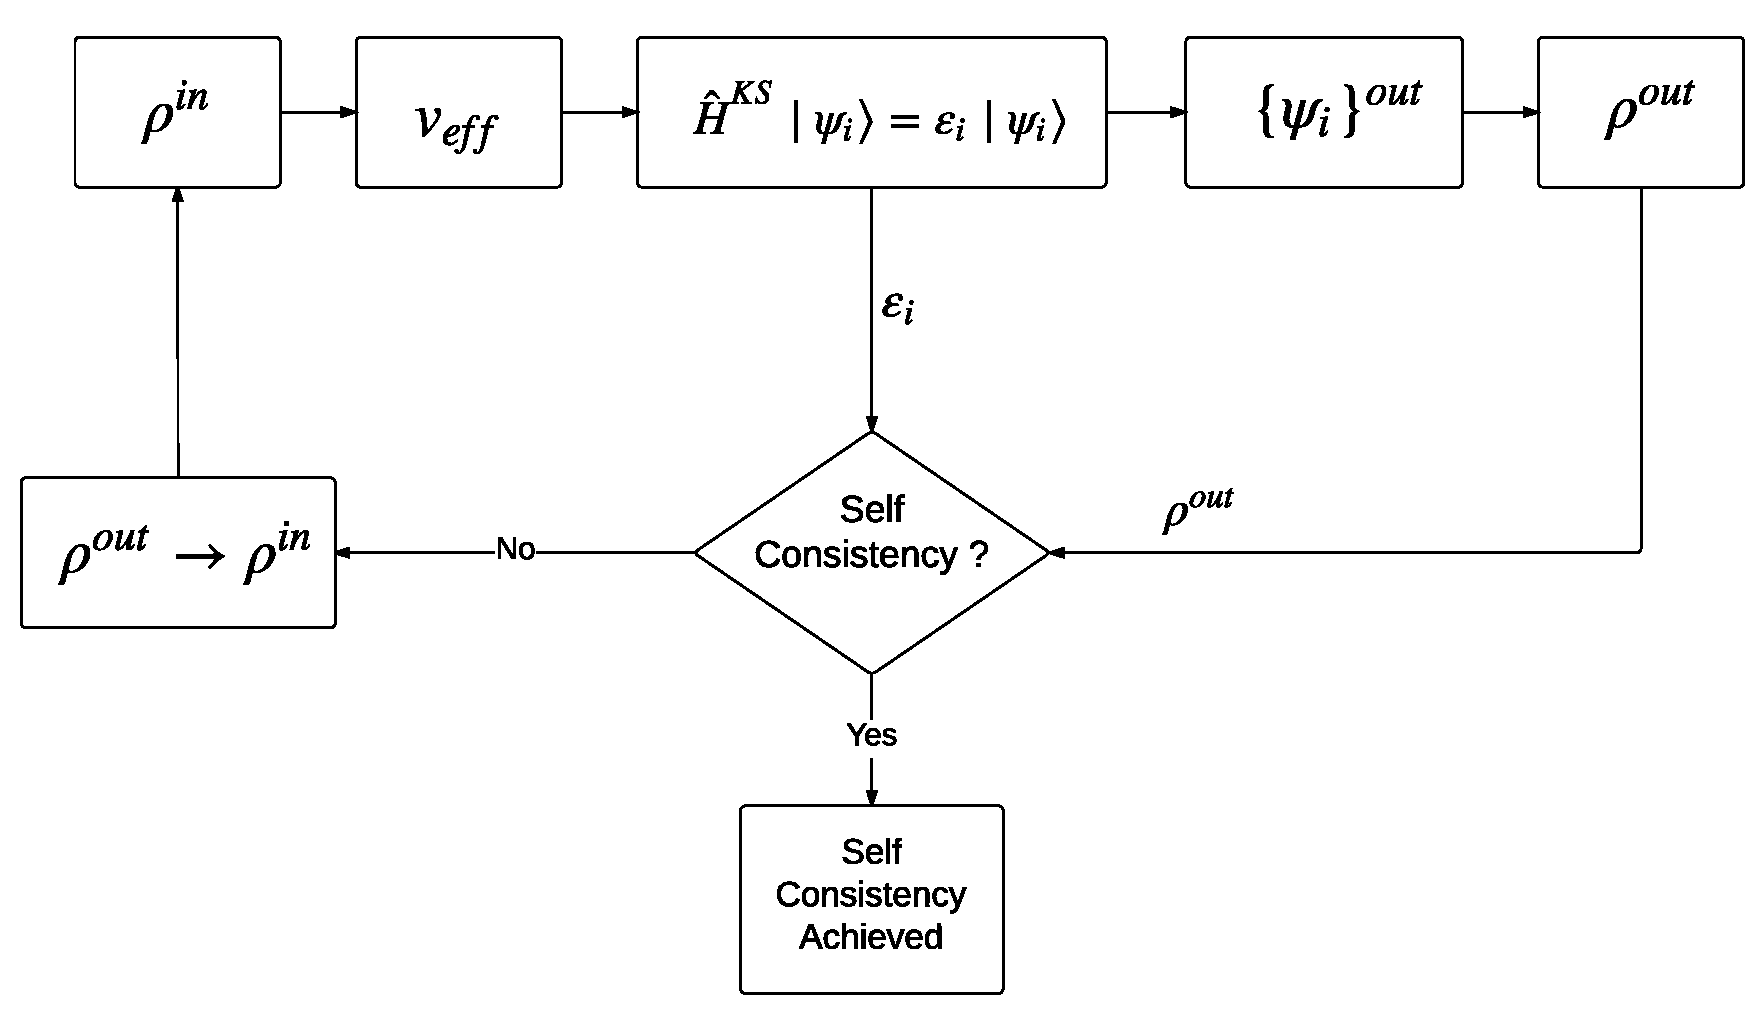
\includegraphics[width=\linewidth]{SCF-DFT_schema.pdf}	
	\end{framed}
	\caption{DFT SCF procedure layout}
	\label{fig:SCF-DFT}
\end{figure}



As one can imagine, the main computational complexity is contained in step \ref{en:SCFDiag}.
The choice of the basis set has great impact on the implementation of this procedure, both for the evaluation of $H \ket{\psi}$ and the diagonalization strategy. 

As a final consideration of this section we must say that the Kohn-Sham eigenvalues $\varepsilon^{KS}_j$ don't posses a physical meaning \cite[p.144]{Martin}, they cannot be associated with \textit{real} energies \footnote{With the exception of the highest $\varepsilon_{i}$ \cite[p.144]{Martin}}. 
The same can be said about the spatial orbitals  $\{\psi^{ks}_j\}$, which are not \textit{real} electronic orbitals. 
Nevertheless they constitute a set of useful tools to build other meaningful physical quantities, first and foremost the electronic density $\dens$.

\subsection{Lattice Structures}
It is convenient to introduce the concept of \textit{Bravais lattice} and \textit{reciprocal lattice} for their central role in solid state physics. 


\subsubsection{Bravais Lattice}
The \textit{Bravais lattice} is a set of points in real space that can be identified by the following relation :
\begin{equation}\label{eq:BravaisLattice}
	\mathbf{R} = n_{1} \mathbf{a}_{1} + n_{2} \mathbf{a}_{2} + n_{3} \mathbf{a}_{3} ,
\end{equation}
where $\{\mathbf{a}_{i}\}$ is as a set of linear independent vectors called the \textit{primitive vectors} and $n_{i}$ is always an integer number.
The definition appears clear looking at figure \ref{fig:BravaisLattice}.

\begin{figure}[h]
\begin{center}
	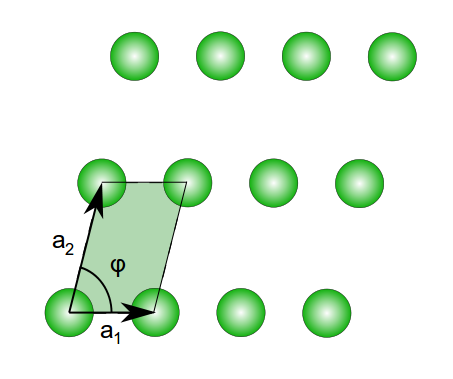
\includegraphics[width=0.4\linewidth]{Bravais_2D.png}
	\caption{Bi-dimensional Bravais lattice, with two of the possible primitive vectors.}
	\label{fig:BravaisLattice}
\end{center}
\end{figure}

Forming a matrix from the primitive vectors, one can express the volume of the primitive cell as 
\begin{align}
	\Omega = det(\left[\mf{a}_1 \mf{a}_2 \mf{a}_3\right]).
\end{align}

\subsubsection{Primitive Cell}
The \textit{primitive cell} is the single smallest portion of lattice that can generate the whole lattice by applying translation and symmetry operations.

\subsubsection{Wigner-Seitz Cell}

The \textit{Wigner-Seitz} cell around a lattice point $\mathbf{R}$ is defined as the locus of points in space that are closer to that lattice point than to any of the other lattice points (see figure \ref{fig:WSCell}).

\begin{figure}[h]
\begin{center}
	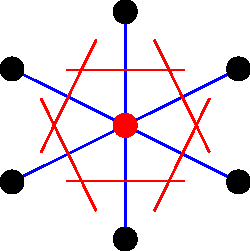
\includegraphics[width=0.4\linewidth]{Wigner.pdf}
	\caption{Bi-dimensional Wigner-Seitz cell}
	\label{fig:WSCell}
\end{center}
\end{figure}

\subsubsection{The Reciprocal Lattice}
Considering a set of $\mathbf{R}$ points constituting a Bravais lattice and a plane wave $\psi(\erre) = e^{i\mathbf{k}\cdot\mathbf{r}}$, for a generic $\mathbf{k} \in \mathbb{R}$ the plane wave $\psi(\erre)$ will be periodic on the lattice only for certain values of $\mathbf{k}$.


We call the ``\textit{reciprocal lattice}" the set $\{\mathbf{K}\}$ of points $\mathbf{k}$ for which the associated plane wave $\psi(\erre)$ is periodic in the Bravais lattice.

One can show \cite{Martin} that the reciprocal lattice is a Bravais lattice and that the following relationship (in matrix form) between the reciprocal primitive vectors $\{\mathbf{b}_i\}$ and the original primitive vectors $\{\mathbf{a}_i\}$ held:
\begin{equation}
\left[\mathbf{b_{1}b_{2}b_{3}}\right]^{T} = (2\pi^3) \left[\mathbf{a_{1}a_{2}a_{3}}\right]^{-1}
.
\end{equation}

A generic point in the reciprocal lattice is identified by the $\mathbf{G}$ vector 
\begin{equation}
	\mathbf{G} = m_1\mathbf{b_1} + m_2\mathbf{b_2} + m_3\mathbf{b_3},
\end{equation}
where $m_i$ is an integer.

Given the periodic condition, every plane wave must satisfy 
\begin{equation}
	e^{i \mathbf{G}\cdot (\mathbf{r} + \mathbf{R})} =  	e^{i \mathbf{G}\cdot \mathbf{r}},
\end{equation}
hence 
\begin{equation}
	e^{i \mathbf{G}\cdot \mathbf{R}} =  	1,
\end{equation}
equivalently 
\begin{align}
	&\mathbf{G}\cdot \mathbf{R} = 2\pi N &N\in\mathbb{Z},
\end{align}
for every $\mathbf{R}$ in the Bravais lattice.

Usually the original Bravais lattice $\{ \mathbf{R} \}$ is called the ``\textit{direct}" lattice.

Finally, the Wigner-Seitz cell of the reciprocal lattice is called the ``\textit{first Brillouin zone}".

As explained in \cite[p.121]{Manini} the reciprocal lattice is the (discrete) Fourier transform of the direct lattice.

We will see that the duality between the direct lattice and the reciprocal lattice is one of the greatest computational strength of theories based on plane waves basis sets.

\subsection{Electrons in Lattice}\label{sec:elLattice}

Solid state physics studies the properties of matter when arranged in crystal lattice form, i.e. each lattice point (or node) accommodate an atom or a molecular structure. 
Elementary cells composed by a group of nodes are then replicated trough translation and symmetry operations to generate the whole crystal.
\subsubsection{The Bloch Theorem}
Since, as we have seen before, the potential the electrons are subjected to is mainly defined by ions' positions\footnote{Remember that the Born-Oppenheimer approximations stands firmly.}, in a lattice we must expect a periodic $v_{eff}$ potential.

Namely, we have that in equation \eqref{eq:KSeq} 
\begin{equation}
	v_{eff}(\erre) = 	v_{eff}(\erre + \mf{R}).
\end{equation}
But what are the implications of this condition on the solutions of \eqref{eq:KSeq}?

The well celebrated \textit{Bloch's theorem} \cite[p.136]{Manini} answers the question.

\begin{center}
\begin{framed}

\textit{All Schr\"odinger eigenstates in a periodic potential $v_{eff}(\erre) = 	v_{eff}(\erre + \mf{R})$ can be chosen in the factorized form:}
\begin{equation}\label{eq:Bloch}
		\psi_{j}(\erre) = e^{i \mf{k} \cdot \erre } ~ u_{\mf{k}j}(\erre), 
\end{equation}
\textit{where the function $u_{\mf{k}j}(\erre)$ has the same periodicity of the lattice $u_{\mf{k}j}(\erre) = u_{\mf{k}j}(\erre + \mf{R}) $, and $\mf{k}$ is a suitable wave vector (depending on $\psi_j$, but otherwise subject to no restriction).}
\end{framed}
\end{center}

Which implies two equivalent considerations.
\begin{itemize}
	\item In a periodic context all electronic eigenfunctions have non-trivial spatial  dependence only within one primitive unit cell: in any other cell the wave function is equal to that in the original cell, apart from a constant phase factor $e^{i \mf{k} \cdot \mf{R}}$ (which leaves the probability distribution unaffected).
	\item In a periodic potential, the Schr\"odinger eigenstates are essentially plane-wave-like states, except for a periodic amplitude modulation.
\end{itemize}

If we substitute \eqref{eq:Bloch} in the Kone-Sham equations \eqref{eq:KSeq} we obtain \cite[p.137]{Manini}
\begin{framed}
\begin{equation}\label{eq:BlochEq}
	\left\lbrace -\frac{1}{2}  \left( \nabla + i\mf{k} \right)^2 + v_{eff}(\erre) \right\rbrace u_{\mf{k}j}(\erre) = \varepsilon_{\mf{k}j}  u_{\mf{k}j}(\erre),
\end{equation}
\end{framed}
which is the basic equation for stationary states of an electron characterized by a given $\mf{k}$.\footnote{Note that this result is the same for every ``\textit{mean field}" approximation (i.e. HF equations)}

The consequence of the Bloch's theorem is that, thanks to the periodicity of $u_{\mf{k}j}(\erre)$, equation \eqref{eq:BlochEq} must be solved within a single cell of the direct lattice\footnote{With applied boundaries conditions}.
This is to be compared with the solution of equations \eqref{eq:KSeq} that must be solved in the \textit{whole} crystal lattice.

Once $u_{\mf{k}j}(\erre)$ is found, the true electronic wave function $\psi_j(\erre)$ is extended to the whole lattice trough \eqref{eq:Bloch}.

Apart for the $\mf{k}$ shift of wave vector, equation \eqref{eq:BlochEq} is equivalent to a stationary Schr\"oendiger equation. Then, for a fixed $\mf{k}$, its solutions must be qualitatively similar to those of standard Schr\"oendiger equations in a finite volume, namely: a ladder of discrete eigenenergies $\varepsilon_{\mf{k}j}$ associated with eigenfunctions $u_{\mf{k}j}(\erre)$ with larger and larger number of nodes for increasing energies, labeled precisely by the index $j$.\footnote{With a noticeable parallelism to atomic orbitals.}

It is absolutely fundamental to note that $\mf{k}$ can vary freely within the first Brillouin zone; 
then for a fixed $j$ the eigenenergies $\varepsilon_{\mf{k}j}$ depends on $\mf{k}$ as \textbf{continuous} functions!

These functions are called ``\textit{energy bands}" or simply ``\textit{bands}", because they varies with $\mf{k}$ within a certain energy interval. 
In general, in solids, bands of contiguous $j$ can either overlap or not; 
thus the main consequence of the Bloch's theorem is that the allowed energies forms a spectrum of bands, separated by ranges of forbidden energies (\textit{band gaps}).

\subsubsection{Plane Waves}
In a crystals, electrons are characterized by an energy spectrum somewhat intermediate between that of a free particle (plane waves with all positive energies) and that of an atom (isolated eigenvalues separated by gaps).

One possible approach to model this kind of behavior is to use plane waves as basis set for the expansion of $\psi_{j}$.
\begin{equation}\label{eq:PWExpansion}
	\ket{\psi_j}  = \sum_{\mf{k}'} c_{j\mf{k}'} \ket{\mf{k}'},
\end{equation}
where $\{\ket{\mf{k}'}\}$ is a set of ortho-normalized plane wave states $\mathbf{k'}(\erre) = \sqrt{V}^{-1} e^{i\mf{k'}\cdot\erre}$ and $c_{j\mf{k}'}$ are the Fourier expansion coefficients.\footnote{Note that in general the sum extends over all possible $\mf{k}'$, leading to an integration:
\begin{equation}
	\psi_j(\erre) = \int \varphi_j(\mf{k}) e^{i\mf{k} \cdot \erre} \dd{\mf{k}}.
\end{equation}
}

Replacing \eqref{eq:PWExpansion} in \eqref{eq:KSeq} and multiplying on the left for $\bra{\mf{k}}$ we obtain \cite{Martin} 
\begin{align}
	\bra{\mf{k}} -\frac{1}{2}\nabla^2 + v_{eff} \ket{\psi_j} &= \varepsilon_j \bra{\mf{k}}\ket{\psi_j},  \\
	\sum_{\mf{k'}} \left( \frac{1}{2}\mid\mf{k}\mid^2  \delta_{\mf{k},\mf{k'}} + \bra{\mf{k}}v_{eff}\ket{\mf{k'}} \right) c_{\mathbf{jk'}} &= \varepsilon_j \sum_{\mf{k'}} \delta_{\mf{k},\mf{k'}} c_{\mathbf{jk'}} \label{eq:SCHFourier},
\end{align}

where we have used $\bra{\mf{k}}\ket{\mf{k'}} = \delta_{\mf{k},\mf{k'}}$ and the fact that $\ket{\mf{k}}$ are eigenstates of the momentum operator.

This is the form equation \eqref{eq:DFTMatrix} takes when plane waves are used as basis set, where $\mathbf{S}$ is diagonal and $\mathbf{C}$ is composed by Fourier expansion coefficients.

Expliciting the matrix element $\bra{\mf{k}} v_{eff} \ket{\mf{k'}}$ we have \cite{Martin} 
\begin{equation}
	\bra{\mf{k}} v_{eff} \ket{\mf{k'}} = \mathcal{N} \int e^{i\left(\mf{k} - \mf{k'} \right) \cdot \erre} v_{eff}(\erre) \dd{\erre} = \tilde{v}_{eff}(\mf{k} - \mf{k'}),
\end{equation}

that are the Fourier components of the potential $v_{eff}$, where $\mathcal{N}$ is the appropriate normalizing constant.

So far we said nothing about the nature of our system, in fact equation \eqref{eq:SCHFourier} is the equivalent formulation of \eqref{eq:KSeq} in Fourier space, where in general $\mf{k}$ are continuous quantities.
This means that by using plane waves we can perform a set of calculations in the reciprocal space, and then transpose the results in the direct space trough inverse Fourier transformations.

If we introduce the condition of a periodic potential, as a consequence of the Bloch's theorem, we have that $\tilde{v}_{eff}(\mf{k} - \mf{k'})$ is not-null only when $\mf{k} - \mf{k'} = \mf{G}$, where $\mf{G}$ is a vector of the reciprocal lattice \cite{Martin}.

This means that in the continuous-indexed energy matrix of equation \eqref{eq:SCHFourier} most off-diagonal elements vanishes because for the element to be not-null the following relation must stand $\mf{k} = \mf{k'} + \mf{G}$.

Then the continuous-indexed $\mf{H}^{KS}$ matrix becomes a diagonal discrete-indexed block matrix, meaning that one can diagonalize only the non-null blocks on the diagonal, and, more importantly, the operation can be performed independently for each block (i.e. in parallel!).

For computational purposes the discrete index is obviously a great advantage, but we still have to address the problem that we need an infinite number of $G$ to completely describe the system.
Following the same process of the Hartree-Fock method, we select only a subset of all the possible plane waves by imposing a condition on the energy of the plane wave, the so-called \textit{cutoff energy}:
\begin{align}
	\mf{k'}(\erre) = e^{i(\mf{k + G}) \cdot \erre};\\
	\frac{\hbar^2}{2m_e}\mid \mf{k + G} \mid < E_{cut}. \label{eq:cutoffEnergy}
\end{align}

In order to pick the correct cutoff energy a series of tests can be performed beforehand with little (and constant) computational effort.

We can now summarize the advantages of plane waves basis sets in periodic potentials:
\begin{enumerate}
	\item It is possible to perform calculations in the reciprocal space and then transpose the result in the direct space. Remember that differentiating in direct space corresponds multiplication in reciprocal space! This greatly simplify the calculation on kinetic terms, and often also of $E_{xc}$.\footnote{As said before, the functional is often expressed in function of $(\dens,\grad\dens,\nabla^2\dens)$.}
	\item The continuous indexed matrix $\mf{H}^{KS}$ becomes a finite discrete-indexed matrix.
	\item The $\mf{H}^{KS}$ matrix becomes diagonal at blocks, and each block can be diagonalized in parallel. \label{en:Kpoints}
\end{enumerate}

Point \ref{en:Kpoints} is the so-called \textit{K-points parallelization}, and, as one can image, it has a great impact on the resolution of the electronic problem in symmetric crystals.

In this work we mainly focused on the study of systems having little symmetries\footnote{Non-periodic systems usually has peculiar physical properties, this is why they are of great research interest and why we focused on them.}, this implies the enlargement of the elementary cell to accommodate all asymmetric factors. 
As a result the $\mf{H}^{KS}$ matrix becomes occupied mostly by a single block and no k-points parallelization can be performed.
This configuration is usually referred as \textit{Gamma point}.



\subsubsection{Grid representation and the size of the problem} \label{sec:Grid}

Thanks to the Bloch's theorem, the calculation for each $\mf{k}$ point is independent and, as said above, we focused on systems in gamma-point configuration. 
%then for the sake of simplicity we will consider $\mf{k}=0$.

Consequently, any of the following considerations is valid within a given (and fixed) k-point sub-block of $\mf{H}^{KS}$.

We know that the solutions to equation \eqref{eq:BlochEq} are in factorized form :
\begin{align}
	\psi_{j}(\erre,\mf{k}) &= e^{i \mf{k} \cdot	 \erre} u_{\mf{k},j}(\erre,\mf{k}), \\
	u_{\mf{k},j}(\erre,\mf{k}) &= \frac{1}{\sqrt{\Omega}} \sum_{\GI} c_{j}(\GI,\mf{k})e^{i \GI \cdot \erre}.
\end{align}

Using the above convention $u_{\mf{k},j}(\erre,\mf{k})$ became:

\begin{align}
	u_{kj}(\erre) = \frac{1}{\sqrt{\Omega}} \sum_{\GI} c_{kj}(\GI)e^{i \GI \cdot \erre},
\end{align}

being $c_{kj}(\GI)$ the Fourier expansion coefficients, it coincides with a discrete Fourier transformation.

The expansion is truncated using equation \eqref{eq:cutoffEnergy} to a certain $\mid \GI \mid < G_{cut}$ (where $G_{cut}$ is the maximum module of a reciprocal vector below the cutoff energy \eqref{eq:cutoffEnergy}), fixing the size of the basis set. This can be done because $v_{eff}$ converge rapidly with increasing modulus of $\GI$.

According to \cite[p.88]{Marx} a rough estimate of the number of plane waves is \footnote{With both $\Omega$ and $E_{cut}$ expressed in atomic units.}
\begin{equation}\label{eq:NGPW}
	N_{G}^{PW} = \frac{1}{2\pi^2}\Omega E_{cut}^{\frac{3}{2}}.
\end{equation}

A function given as a finite linear combination of plane waves can also be defined as a set of functional values on an equally spaced grid in real space.

The real space sampling points $\mf{R}$ are defined as: 

\begin{equation}
	\mf{R} = \left[\mf{a}_1 \mf{a}_2 \mf{a}_3 \right] \mf{N} \mf{q},
\end{equation}

where N is a diagonal matrix with the entries $1/N_i$, $\mf{q}$ is a vector of
integers ranging from $0$ to $N_i - 1$ and $i = x, y, z$. 

To prevent the loss of any information contained in the function\footnote{Respecting the sampling theorem.}  $N_i$ has to be bigger than $2 max(\mf{b}_i) + 1$\footnote{Where $\mf{b}_i$ is a primitive vector of the reciprocal lattice}. 
In addition, $N_i$ must be decomposable into small prime numbers (typically 2, 3, and 5) when fast Fourier transformation techniques are used.
In practice, the smallest number $N_i$ that fulfills the above requirements is
chosen.

A periodic function can be calculated at the real space grid points $\mf{R}$ as \cite[p.89]{Marx} :
\begin{align}
	f(\erre) &= \sum_{\GI} \tilde{f}(\GI) e^{i \GI \cdot \erre} \\
			 &= \sum_{\mf{b}} \tilde{f}(\GI) exp\left[ \frac{2\pi}{N_{x}} i b_x q_x \right]  exp\left[ \frac{2\pi}{N_{y}} i b_y q_y \right]  exp\left[ \frac{2\pi}{N_{z}} i b_z q_z \right], \label{eq:FFTDef}
\end{align}
where we have expanded every $\GI$ in a linear combination of the primitive reciprocal vectors $\{\mf{b}_i\}$.

The function $\tilde{f}(\GI)$ is zero outside the cutoff region, and the sum over the \textbf{b}-vectors can be extended over all indices in the cube $-\mf{b}_{i}^{max} , \cdots ,\mf{b}_{i}^{max}$ . 

The functions $f(\mf{R})$ and $\tilde{f}(\GI)$ are related
\begin{align}
	f(\mf{R}) &= IFT[ \tilde{f}(\GI) ]\\
	\tilde{f}(\GI) &= FT[ f(\mf{R}) ].
\end{align}

The calculation of the three-dimensional Fourier transforms can be performed by a
series of one-dimensional Fourier transforms \cite{Marx}. The number of transforms in
each direction is $N_y N_z$ , $N_x N_z$ , and $N_x N_y$ , respectively. Assuming that the
one-dimensional transforms are performed within the fast Fourier transform
framework, the number of operations per transform of length $n$ is approximately $\mathcal{O}(n log(n))$. This leads to an estimate for the number of operations for the full three-dimensional transform of $\mathcal{O}(N log(N))$ , where $N = N_x N_y N_z$ .

Because to use the FFT a regular grid in the form of a parallelepiped is needed (both in direct and reciprocal space), the number of points in the FFT grid for density $N = N_{R} = N_{G}$ is roughly an order of magnitude larger than the number $N_{G}^{PW}$ defined in \eqref{eq:NGPW} \cite{Martin}.

See table \ref{tab:FFTSummary} for a summary of the relationships between direct and reciprocal grid and an estimate of their typical dimensions.

\begin{table}[]
\centering
\begin{tabular}{lc}
\hline
\multicolumn{1}{|l|}{\textbf{Size}} & \multicolumn{1}{l|}{\textbf{Description}}                                                                                                                        \\ \hline
\multicolumn{1}{|l|}{$N_{R}$}       & \multicolumn{1}{l|}{Number of $\mf{R}$ points in the real grid}                                                                                                  \\ \hline
\multicolumn{1}{|l|}{$N_{G}$}       & \multicolumn{1}{l|}{Number of $\GI$ points in the reciprocal grid}                                                                                               \\ \hline
\multicolumn{1}{|l|}{$N_{G}^{PW}$}  & \multicolumn{1}{l|}{\begin{tabular}[c]{@{}l@{}}Number of $\GI$ points in the reciprocal grid associated to \\ plane waves below the cutoff energy\end{tabular}} \\ \hline

                                    & \multicolumn{1}{l}{}                                                                                                                                             \\ \cline{2-2} 
\multicolumn{1}{l|}{}               & \multicolumn{1}{c|}{\textbf{Relationships}}                                                                                                                      \\ \cline{2-2} 
\multicolumn{1}{l|}{}               & \multicolumn{1}{c|}{$N_{R} = N_{G} = N = N_x N_y N_z$}                                                                                                                         \\ \cline{2-2} 
\multicolumn{1}{l|}{}               & \multicolumn{1}{c|}{$N_{G}^{PW} < N$}                                                                                                                       \\ \cline{2-2} 
\multicolumn{1}{l|}{}               & \multicolumn{1}{c|}{\textbf{Estimate for a 100 atom system}}                                                                                                                       \\ \cline{2-2} 
\multicolumn{1}{l|}{}               & \multicolumn{1}{c|}{ $N_{b} \simeq \frac{1}{2} N_{e^{-}} \simeq 10^3~;~ N_{G}^{PW} \simeq 10^{6} ~;~ N \simeq 10^7 $}                                                                                                                       \\ \cline{2-2} 
                                    &                                                                                                                                                                  \\ \cline{2-2} 
\multicolumn{1}{l|}{}               & \multicolumn{1}{c|}{\textbf{Computational cost of every Fast Fourier Transform}}                                                                                           \\ \cline{2-2} 
\multicolumn{1}{l|}{}               & \multicolumn{1}{c|}{$\mathcal{O}(N log (N))$}                                                                                                                    \\ \cline{2-2} 
\end{tabular}
\caption{Summary of typical dimensions between direct and reciprocal grid}
\label{tab:FFTSummary}
\end{table}



We shall now proceed with an in-depth analysis of the implementation of DFT SCF methods in the Quantum ESPRESSO suite, one of the most popular and solid software for materials modeling.


\newpage

~

\newpage
%----------------------------------------------------------------------------
\section{\QE}\label{sec:QE}
%----------------------------------------------------------------------------

\QE  is an integrated suite of computer codes for electronic-structure calculations and materials modeling based on density-functional theory, plane waves basis sets and pseudopotentials to represent electron-ion interactions.

\QE is free, open-source software distributed under the terms of the GNU General Public License (GPL) and is written, mostly, in Fortran-95, with some parts in C or in Fortran-77.

\QE core features are implemented leveraging the well optimized versions of linear algebra and parallelization libraries like BLAS\cite{BLAS}, LAPACK\cite{LAPACK}, ScaLAPACK\cite{SCALAPACK}, FFTW\cite{FFTW}, that are easily available for a wide range of computational architectures.

The MPI standard\cite{MPI} is used for interprocess communication and the OpenMP standard\cite{OMP} is used for thread parallelization.


\QE has been compiled and tested on numerous computing systems\cite{QEManual}: i386 Linux desktops, i386 Linux clusters, Mac OS X, Cray machines, IMB AIX, IBM BlueGene, NUMA machines, Intel-Phi co-processors, CUDA accelerators, FPGA accelerators and even mobile devices. 

Quantum ESPRESSO distribution is composed by a set of packages (executables) built upon a versatile core library, a complete list of executables and various features can be found in \cite{QE}.

In our work we focused only on the \textit{PWscf} package, which implements an iterative approach to reach self-consistency, using at each step iterative diagonalization techniques, in the framework of plane waves basis set.

As a note: in this work we will conform to the MPI standard calling each MPI process an \textit{MPI rank} and each group of MPI ranks a \textit{communicator}.

\subsection{SCF Implementation in \textit{PWscf} package}
In section \ref{sec:SCF-DFT} we gave a basic representation of an SCF algorithm based on DFT.

In section \ref{sec:elLattice} we saw how the choice of plane waves as basis set impacts on the solution of Kohn-Sham equations.

Finally, in section \ref{sec:Grid} we showed how direct and reciprocal space are represented and how it's possible to move from one representation to another. 
\QE leverages this feature to calculate the terms in $\mf{H}^{KS}$ where it is more convenient to.


In the following section we will show the calculations needed to perform each SCF step as implemented in PWscf package.

As a reference, we will use  the steps outlined in figure \ref{fig:SCF-DFT} on page \pageref{fig:SCF-DFT}.
The figure is reprinted here to help the reader.

\begin{figure}[h]
\begin{center}
	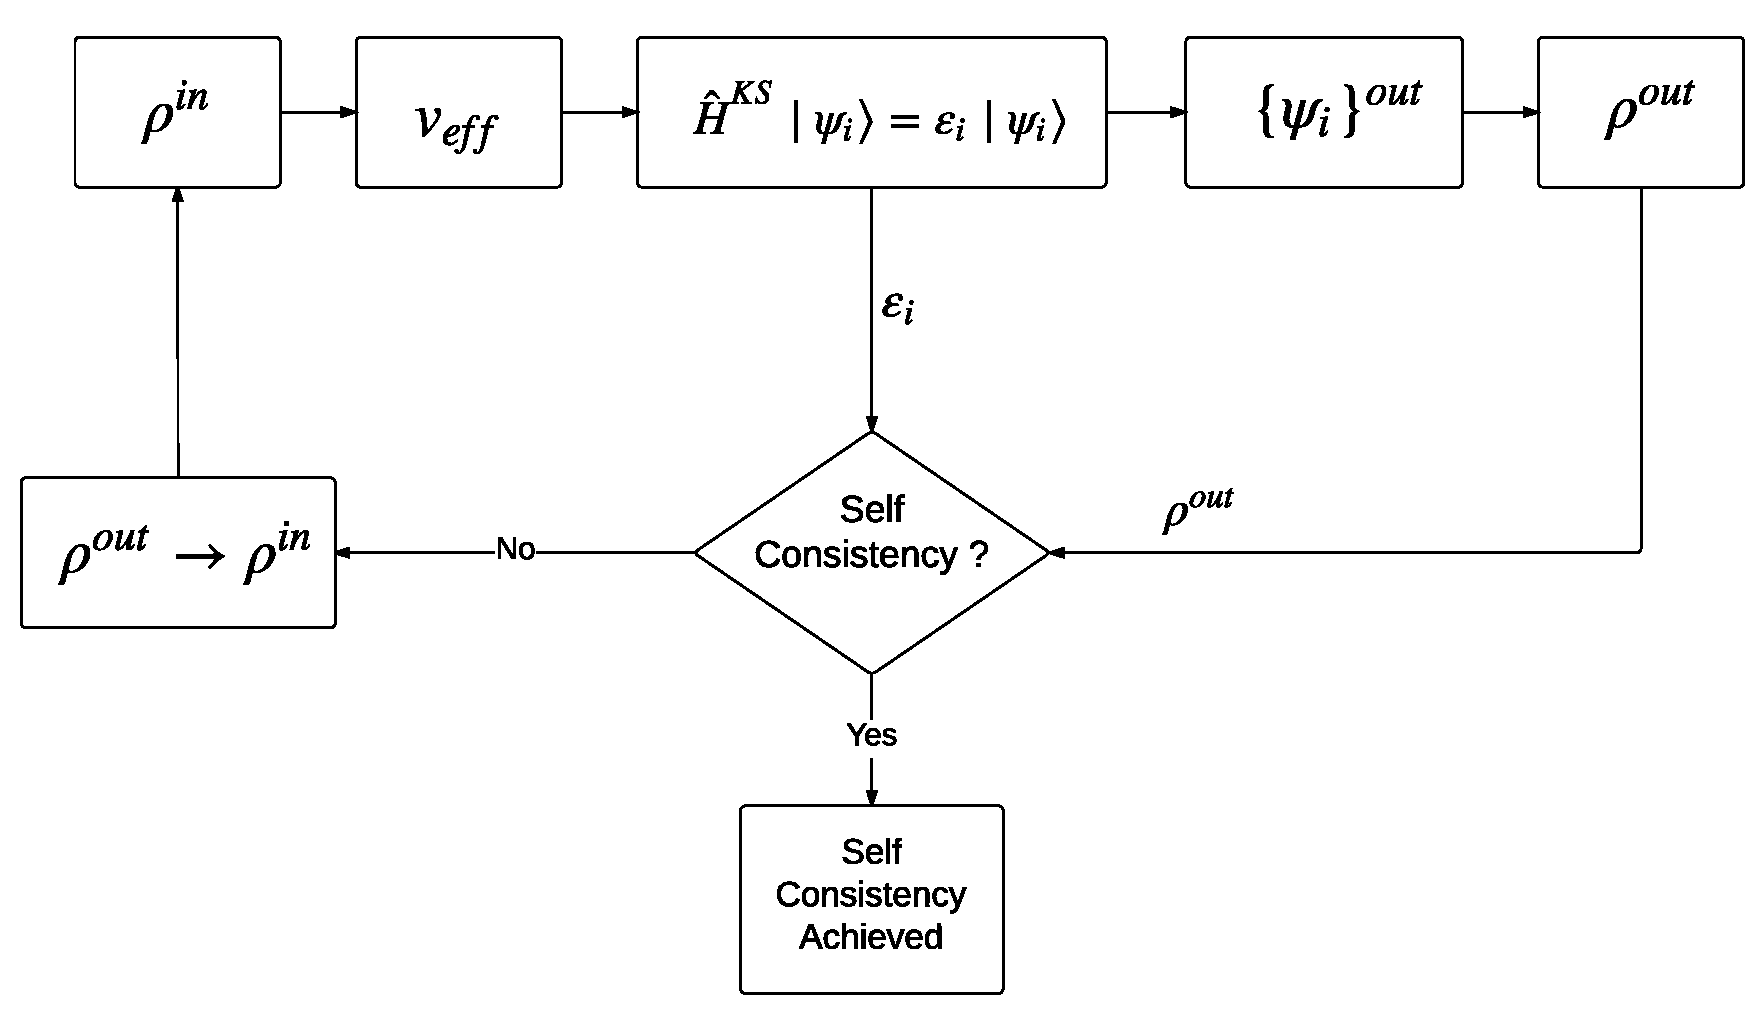
\includegraphics[width=\linewidth]{SCF-DFT_schema.pdf}	
	\end{center}
\end{figure}

\subsection{Initialization (Step 0)}
For the SCF iteration to be performed, a set of preliminary initializations must occur.
This preliminary step is implemented within the \texttt{init\_run} subroutine.

Besides the allocation of all the buffers and the tuning of grid dimensions\footnote{Remember that for the FFT to perform well, the number of points per dimension must be a multiple of a prime number, see sec \ref{sec:Grid}}, the real goal of this step is to obtain an initial electronic density $\dens$ and an estimate of the total energy of the system.

As a default behavior, \QE combines the electronic densities of every atomic species within the elementary cell.
The same is done for the atomic orbitals, composing a preliminary set of Kohn-Sham orbitals $\{\psi_j\}$.
\footnote{This is the default behavior of \QE ,it is also possible to perform a random initialization.}

Using $\dens$ to evaluate $v_{eff}$ and $\{\psi_j\}$ to compute $\mf{H}_{ij}^{KS}$, $\mf{H}^{KS}$ is diagonalized to obtain the initial energy of the system thanks to equation \eqref{eq:DFTEnergy}. 

The results of this preliminary step will be used as a starting point in points one, two and four of figure \ref{fig:SCF-DFT}.

Note that this first diagonalization is much faster than the ones performed during the SCF iteration.




\subsubsection{Evaluating the potential (Step 1)}\label{sec:Potential}

The potential $v_{eff}$ is composed by three terms:
\begin{equation}
	v_{eff} = v + v_{h} + v_{xc},
\end{equation}
where $v$ is the electron-ion potential, $v_{h}$ the electrostatic Hartee potential and $v_{xc}$ is the exchange-correlation potential\footnote{The ``spatial" dependency of the potentials will be explicited when needed.}.

\paragraph{The electron-ion potential:}
$v$ was originally defined in \eqref{eq:electronionPotential} considering every ion as a point-like distribution of charge. 
However, since we choose plane waves as basis set, modeling the behavior of electrons in the valence band (strongly localized around each ion) is rather difficult due to the delocalized nature of plane waves.

Nevertheless plane waves suit greatly the description of electrons in the conduction bands: since the ionic potential they are subject to is screened by valence electrons\cite[p.136]{Manini}, they result more delocalized, especially in lattice crystals.

To model this dual nature without having to enlarge wildly the basis set to describe valence electrons\footnote{i.e. using an high number of Fourier coefficients in \eqref{eq:PWExpansion}, hence a large cutoff energy.}, \QE uses the so-called \textit{pseudopotentials} theory.

A discussion on the nature of pseudopotentials is out of the scope of this work, however a good dissertation on the matter can be found in \cite[chap. 11]{Martin} and \cite[p.90]{Marx}.
What we need to know about pseudopotentials is that the electron-ion potential generated by a single ion can be expressed in reciprocal space as :
\begin{equation}
	\tilde{v}_{\alpha}(\mf{G}) = \sum_{\mf{G}} f_{ps}^{sp}(G) e^{i \mf{G} \cdot \mf{R}_{\alpha}},
\end{equation}
where  $\mf{R}_{\alpha}$ is the position of the ion and $f_{sp}^{sp}(G)$ is the function describing the pseudopotential of the given atomic species ``\textit{sp}" (e.g. hydrogen, oxygen, sodium, ...).

Given the position of each ion within the elementary cell and its atomic species, $\tilde{v}(\mf{G})$ is calculated as a superposition of each $\tilde{v}_{\alpha}(\mf{G})$.

Note that because ions' position is fixed under the Born-Oppenheimer approximation, $\tilde{v}(\mf{G})$ is calculated only once for the whole SCF iteration, then its impact on the computational cost is negligible.  

As said above, the calculation of $\tilde{v}(\GI)$ happens inside the \texttt{init\_run} routine in the first evaluation of $v_{eff}$.



\paragraph{The Hartree Potential:}

$v_{h}(\erre)$ is defined in \eqref{eq:HartreePot} as 
\begin{equation}
 v_{h}(\erre) = \int \frac{\rho(\mathbf{r'})}{\mid \mathbf{r} - \mathbf{r'} \mid}  \dd{\mathbf{r'}}.
\end{equation}

$v_{h}$ is nothing else than the classical electrostatic potential generated by a tridimensional distribution of charge with volumetric charge density $\rho(\erre')$.

We know that every electrostatic potential must satisfy the Poisson's equation :
\begin{equation}\label{eq:Poisson}
	\nabla^2 v_{h}(\erre) = - \frac{\dens}{\varepsilon_{0}},
\end{equation} 
where $\varepsilon_{0}$ is the dielectric constant $(4\pi e^2)^{-1}$.

Equation \eqref{eq:Poisson} in reciprocal space becomes:
\begin{equation}\label{eq:HartreePotReciprocal}
	\tilde{v}_{h}(\mf{G}) = \frac{\tilde{\rho}(\mf{G})}{G^2 \varepsilon_{0}},
\end{equation}
where $\tilde{v}_{h}(\mf{G})$ and $\tilde{\rho}(\mf{G})$ are the Fourier transforms respectively of $v_{h}(\erre)$ and $\dens$.

Instead of having to compute the integral in \eqref{eq:HartreePot}, we just need the expression of $\tilde{\rho}(\mf{G})$.
This is undoubtedly a great advantage from a computational standpoint, because all the complexity lies in the evaluation of $\tilde{\rho}(\mf{G})$, which is performed at the beginning of every iteration step as an FFT of $\dens$.
Hence the computational cost associated to $v_{h}$ is $\bigO(N log(N))$.

Using the definition \eqref{eq:HartreePot} would require to compute the integral for every point of the real grid. 
That is: for every of the $N$ point of the real grid (labeled by $\mf{r}$) one must sum (integrate) again for every point of the real grid $N$ (labeled by $\mf{r}'$). 
This would lead to a complexity of $\mathcal{O}(N^2)$.

For the sake of simplicity we can derive equation \eqref{eq:HartreePotReciprocal} in one dimension.

\begin{equation} \label{eq:PossionMono}
	\pdv[2]{v_{h}(x)}{x} = - \frac{\rho(x)}{\varepsilon_0},
\end{equation}
then 
\begin{align*}
	v_{h}(x) &= \frac{1}{\sqrt{2\pi}} \int \tilde{v}_{h}(g) e^{i g x} \dd{g}; \\
	\rho(x) &= \frac{1}{\sqrt{2\pi}} \int \tilde{\rho}(g) e^{i g x} \dd{g}.
\end{align*}

Replacing into  \eqref{eq:PossionMono} and differentiating, we obtain :
\begin{equation}
	\frac{g^2}{\sqrt{2\pi}} \int \tilde{v}_{h}(g) e^{i g x} \dd{g} = \frac{1}{\varepsilon_{0}\sqrt{2\pi}} \int \tilde{\rho}(g) e^{i g x} \dd{g},
\end{equation}
hence 
\begin{equation}
	\tilde{v}_{h}(g) = \frac{\tilde{\rho}(g)}{g^2 \varepsilon_{0}}.
\end{equation}



\paragraph{Exchange correlation potential:} 
As explained in section \ref{sec:SCF-DFT}, $E_{xc}[\dens]$ is fixed at the beginning of the SCF iteration and never changes trough the whole iteration. $v_{xc}(\erre)$ is obtained analytically trough equation \eqref{eq:ExchangePotDer}.

Even if $v_{xc}(\erre)$ is computed at the beginning of each iteration step, because $E_{xc}[\dens]$ depends on the electronic density, the computational cost of \eqref{eq:ExchangePotDer} is negligible.


~


We now have an expression for all the terms in $v_{eff}$, but two of them ($\tilde{v}_{h}$ and $\tilde{v}$) are calculated in the reciprocal space.

Since $v_{eff}$ is applied in the direct space, where it's a trivial multiplicative operator, we need to inverse transform $\tilde{v}_{h}$ and $\tilde{v}$.

We have that
\begin{equation}
	v_{eff}(\erre) = IFFT\{\tilde{v}(\mf{G})\}(\erre) + IFFT\{\tilde{v}_{h}(\mf{G})\}(\erre) + v_{ex}(\erre).
\end{equation}

This operation is performed once for every iteration step.

\subsubsection{The kinetic term}\label{sec:KineticTerm}

Another great advantage of plane waves is that differentiation against the state function becomes a mere multiplication in reciprocal space.

In fact we have that 
\begin{equation}
	\nabla^2 u_{kj}(\erre) = \sum_{\mf{G}} - c_{kj}(\mf{G})  G^2  e^{i \GI  \cdot \erre}.
\end{equation}


\subsection{Diagonalization (Step 2)}\label{sec:Diagonalization}
The diagonalization of $\mf{H}^{KS}$ is the core problem of any SCF implementation.

As specified in \cite[Appendix A.2]{QE}, the strategy adopted by \QE is to use the \textit{Davidson method}\cite{Davidson}\footnote{\QE has also an alternative algorithm, called the \textit{conjugate gradient} method.}.

The Davidson method follows an iterative approach to the solution of the eigenvalue problem.
One of the great advantages of this method is that it is possible to obtain the set of the $n$ eigenvectors with the lower (or upper) eigenvalues without performing the diagonalization of the whole $\mf{H}^{KS}$ dense matrix of dimension $N_{G}^{PW} \cdot N_{G}^{PW} \simeq N^2$.

Instead, the $\mf{H}^{KS}$ matrix is reduced in a smaller matrix which generic element is 
\begin{equation}\label{eq:DavidsonMatrix}
	\mf{H}_{ij} = \bra{u_{ki}}\mf{H}^{KS}\ket{u_{kj}},
\end{equation}
where $\ket{u_{kj}}$ is a trial eigenvector. 
Then the size of the matrix is reduced to $N_{b}^2$, to be diagonalized with standard techniques implemented in \QE using LAPACK or SCALAPACK libraries.
This drastically decreases the amount of memory needed to perform the diagonalization.

From equation \eqref{eq:DavidsonMatrix} we can see that for the algorithm to work it is necessary to implement just one basic operation: the application of the matrix to a generic state vector
\footnote{The braket calculation $ \bra{u_{ki}} (\mf{H}^{KS}\ket{u_{kj}})$ is trivial using LAPACK or SCALAPACK libraries.}
\begin{equation}
	\mf{H^{KS}} \ket{u_{kj}}.
\end{equation}
In \QE this operation is implemented inside the well-named subroutine \texttt{h\_psi} and is performed in the reciprocal space (see figure \ref{fig:hpsi}).

The evaluation of $\mf{H^{KS}}$ is divided in the kinetic term $\nabla^2$ and the potential term $v_{eff}$, each term is applied sequentially; 
the trial eigenvectors $\{\ket{u_{kj}}\}^{in}$  are the ones obtained in the previous SCF step, if any, or the ones obtained from \texttt{init\_run}.
\footnote{When the SCF step has converged, the $\{\ket{u_{kj}}\}^{out}$ obtained are not subjected to mixing, unlike $\densout$. The reason is that the amount of memory needed to store them would be too much. 
As a matter of fact $\densin$ can not be generated from $\{\ket{u_{kj}}\}^{in}$.
This in not important because the Davidson method, which is iterative, will guarantee the convergence to the real $\{\ket{u_{kj}}\}^{out}$. 
$\{\ket{u_{kj}}\}^{in}$ have to be considered as a reasonable guess of the new eigenstates $\{\ket{u_{kj}}\}^{out}$, reducing the number of Davidson steps required to reach convergence.
}

As we said in section \ref{sec:KineticTerm}, the application of the kinetic term in the reciprocal space accounts just for a multiplication over $N^{PW}_G$.

In section \ref{sec:Potential} we showed that $v_{eff}(\erre)$ is calculated once per SCF iteration step, then it is fixed during the whole Davidson iteration. Since we are in the reciprocal space but $v_{eff}$ is multiplicative only in real space it is necessary to: 
\begin{enumerate}
	\item transform $\tilde{u}_{jk}(\GI)$ in $u_{kj}(\mf{R})$ using IFFT;
	\item multiply $v_{eff}(\mf{R})$ for $u_{kj}(\mf{R})$ for every $\mf{R}$ in the real grid;
	\item transform the result in reciprocal space : \\ $[v_{eff}(\mf{R}) u_{kj}(\mf{R})](\GI) = FFT\{v_{eff}(\mf{R}) u_{kj}(\mf{R})\}$;
\end{enumerate}

\begin{figure}[h]
\begin{center}
	\begin{framed}
	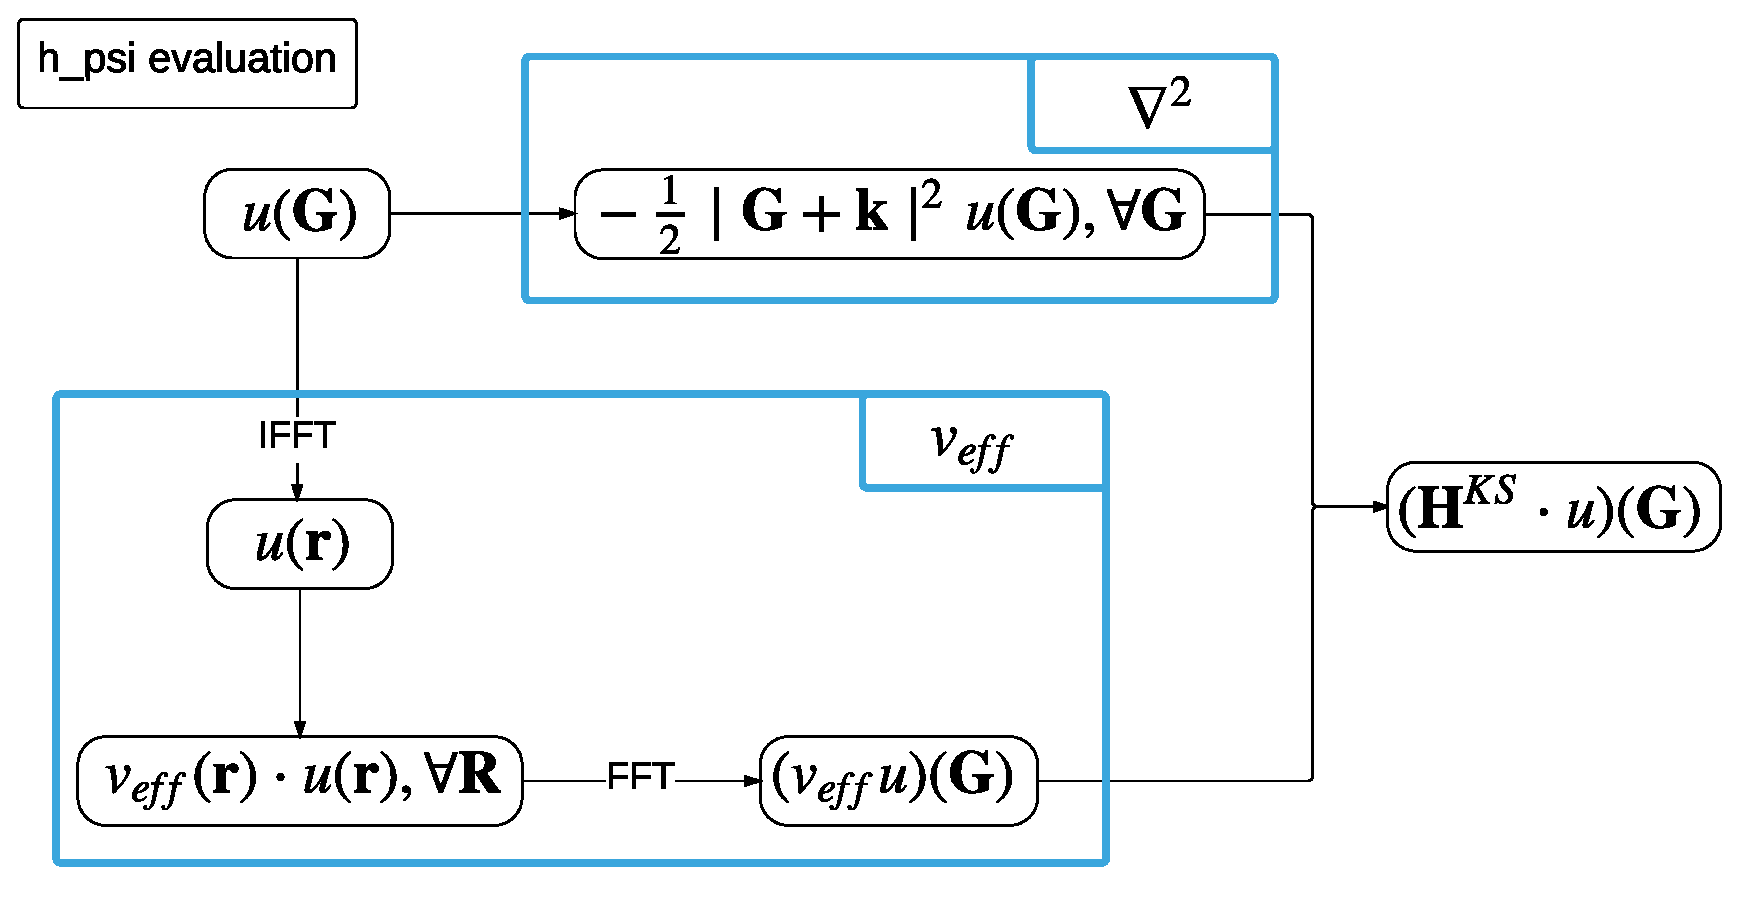
\includegraphics[width=\linewidth]{h_psi.pdf}

	\end{framed}
\caption{Implementation of \texttt{h\_psi} subroutine in \QE}
	\label{fig:hpsi}
\end{center}
\end{figure}


This means that for every call of \texttt{h\_psi} an FFT and an IFFT must be performed, each of them with complexity $\bigO(N log (N))$. 

Since \texttt{h\_psi} is called once over all the $\{u_{kj}\}$, the total complexity per iteration step is $\bigO(N_{b} N log (N))$, where $N_{b}$ is the number of bands (that is of the order of the number of electrons in the system\footnote{Neglecting spin effects, $N_b = 1/2 N_e$.}). 

Note that this is the complexity of a single Davidson iteration, the number of iterations required to solve the eigenvalue problem cannot be predicted beforehand but the computational cost of the whole Davidson diagonalization\footnote{Excluding the evaluation of $\mf{H}^{KS}$} goes as $\bigO(N_{b}^3)$ and is usually accounted as the global computational complexity of the whole DFT-SCF computation.

\subsubsection{FFT implementation}\label{sec:FFT}
Given their central role, it is convenient to outline how FFT transformations are performed inside \QE .
We can explicitly rewrite equation \eqref{eq:FFTDef} for an IFFT from reciprocal to real grid.

\begin{align}
	IFFT[f(\GI)] &= \sum_{j}^{N_x} \sum_{k}^{N_y} \sum_{l}^{N_z} f^{\GI}_{jkl}
		exp \left[i \frac{2\pi}{N_x}ju \right] 
		exp \left[i \frac{2\pi}{N_y}kv \right] 
		exp \left[i \frac{2\pi}{N_x}lw \right] \\
		[u,v,w] &= \mf{q} \\
		[j,k,l] &= \mf{b}_i.
\end{align}
This factorized form can be implemented as a series of three nested cycles, one for each dimension.
Usually the cycle on the $z$ axis (index $l$) is the first to be performed:
\begin{equation}\label{eq:NestedFFT2}
	IFFT[f(\GI)] = \sum_{j}^{N_x} \sum_{k}^{N_y} 
		exp \left[i \frac{2\pi}{N_x}ju \right] 
		exp \left[i \frac{2\pi}{N_y}kv \right] 
		\sum_{l}^{N_z} 	f^{\GI}_{jkl} exp \left[i \frac{2\pi}{N_x}lw \right].
\end{equation}
What \QE does is to divide the grid in a set of $N_x \cdot N_y$ columns along the $z$ axis, then the sum is performed in parallel for each column. 
This parallelization is implemented using MPI, that is : each rank calculates sequentially a set of columns.
Since the terms in the rightmost sum in \eqref{eq:NestedFFT2} are independent from one another, the sum over each column can be parallelized. 
This second layer of parallelization is performed using thread parallelization, thanks to the OpenMP library.
Being every term independent, there are no race-conditions between threads, they do not need to wait the computation performed by other threads and they work on independent chunks of memory. \footnote{See appendix \ref{app:Threads} for the effects of threads overload.}

Once the sum on z columns is completed, the grid is separated in horizontal layers. 
The layers are grouped in function of the MPI ranks and bidimensionals FFT are perfomed; the second thread parallelization can still be used.

\QE uses the well known library FFTW (``Fast Fourier Transform in the West")\cite{FFTW} to perform one dimensional transformations. 
Even if a native parallel implementation of tridimensional transformations was developed in FFTWv3, \QE uses his own parallelization strategy. 
This design was developed when architectures like CrayAX an Sun HPC solutions where still supported. It was common for this kind of architectures to expose native and well optimized implementations of one-dimensional FFT transformations.

\subsubsection{Dense matrices diagonalization}

As said above, the Davidson method reduces the problem to the diagonalization of a $N_{b}^2$ matrix.
\QE can perform this operation either in parallel or serially.
The kind of parallelization used can be manually set or automatically decided.

\paragraph{Serial diagonalization: }  In this case, only one MPI rank performs the diagonalization.
\footnote{Actually, depending on the version of \QE, a set of different ranks would perform the same operation, obtaining the same result.}
Be aware that thread parallelization is still an option, if threads are enabled and the threaded version of MKL libraries have been linked.
See section \ref{sec:resArchIndependent} for an test case analysis of this scenario.

\paragraph{Parallel Diagonalization: } In this case \QE leverages the features of the SCALAPACK library and distribuite the load over a set of MPI ranks. 
Not all the ranks will be used: depending on the total number of ranks or on user setting, a number ranging from one-forth to one-half of ranks will be used. 
These ranks will be equally spaced and distributed over the whole computational resource, this is done to prevent the overload of the memory controller of a single machine.
Thread parallelization can still be performed, as noted above.


\subsection{Calculation of the electronic density (Step 3)}

After Davidson's diagonalization is concluded, a set $\{ u_{kj}(\GI) \}$ of $N_{b}$ eigenstates with the lowest energy is obtained.

To calculate the final density in real space it is convenient to use equation \eqref{eq:densityDef}, but, to do so, one need to transform $\{ u_{kj}(\GI) \}$ in $\{ u_{kj}(\erre) \}$ using an IFFT \cite[p.246]{Martin}.

The IFFT transform constitute the major computational cost, and it's comparable with the cost of a single Davidson step.

The procedure is implemented inside the routine \texttt{sum\_band}, which is also responsible for the computation of occupations and the sum of eigenvalues.


\subsection{Convergence criteria (Step 4)}\label{sec:SCFConvergence}
As explained in \ref{sec:SCF-DFT} a set of convergence test can be performed on $\densout$ and $E[\densout]$.
\QE uses a refined methods that estimates the impact of the difference between $\densout$ and $\densin$ on the energy of the system.
First we define the difference between $\densout$ and $E[\densout]$ as 
\begin{equation}
	\Delta\dens = \densin - \densout.
\end{equation}
Then we consider the terms in $E[\dens + \Delta\dens] - E[\dens ]$ which are quadratical in $\Delta\dens$ \footnote{Linear terms are zero in proximity of the minimum.} :
\begin{align}
	\Delta E = E[\dens + \Delta\dens] - E[\dens ] &\simeq \frac{e^2}{2} \iint \frac{\Delta\rho(\erre) \Delta\rho(\erre')}{\mid \erre - \erre' \mid} \dd{\erre} \dd{\erre'}\\
	 &= \int \Delta\dens \Delta v_{h}(\erre') \dd{\erre},
\end{align}
where we have not consider the second order derivative of $E_{xc}$ because of his complexity.
As a result the only second order contribution to the energy difference is in the Hartree energy.

Convergence is achieved when $\Delta E$ is lower than the parameter \texttt{conv\_thr}\footnote{Default value is $10^-6$ Rb.}.

\subsection{Density mixing (Step 5)}
In the most primitive approach one could use $\densout$ as the $\densin$ for the next SCF step. In reality this approach is not recommended because it won't lead to a fast convergence of the whole SCF iteration\footnote{It can lead to no convergence at all.}.

What \QE does is to mix the value of $\densout$ with the values of the $n=1,..,8$ previously obtained densities.

The details of how the mixing is performed can be found in \cite{Johnson} and the subroutine implementing this operation is called \texttt{mix\_rho}.

The computational cost of this operation roughly goes as the size of the grid ($\bigO(N)$) and it's definitely negligible.


\subsection{Brief comparison with Hartree-Fock method}
In table \ref{tab:HF-DFTComp} we perform a comparison between two of the most popular computational model in solid state physics: DFT SCF algorithm using plane waves as basis set and HF SCF algorithm using Gaussian orbitals.


\begin{table}[h]
\centering
\begin{tabular}{l|l|ll|l|}
\cline{2-2} \cline{5-5}
                                    & \textbf{DFT-PW}        &                       &                    & \textbf{HF-Gaussian} \\ \cline{1-2} \cline{4-5} 
\multicolumn{1}{|l|}{\textbf{FFT}}  & $\bigO(N_{b}N ln(N) )$ & \multicolumn{1}{l|}{} & $\mf{H}_{ij}$ & $\bigO(N_{gauss}^4)$ \\ \cline{1-2} \cline{4-5} 
\multicolumn{1}{|l|}{\textbf{DIAG}} & $\bigO(N_{b}^3)$       & \multicolumn{1}{l|}{} & \textbf{DIAG}      & $\bigO(N_{b}^3)$     \\ \cline{1-2} \cline{4-5} 
\end{tabular}
\caption{Comparison of computational complexity between DFT method using plane waves and HF method using Gaussian orbitals. $\mf{H}_{ij}$ stands for the evaluation of the Hamiltonian(mainly the Fock operator), \textbf{DIAG} is the cost of the diagonalization, $N_b$ is the number of bands, $N_{gauss}$ is the number of Gaussian orbitals in the basis set.}
\label{tab:HF-DFTComp}
\end{table}

The main complexity of the HF method is $\bigO(N^4)$\footnote{N is the size of the HF basis set.}, and rises from the evaluation of the exchange terms in the Fock matrix (see section \ref{sec:FockMatrix}). 
What usually is not mentioned is that this is just the complexity of the evaluation of the Fock matrix, every HF method has still to perform the diagonalization\footnote{Which, depending on the algorithm, can have a complexity ranging from $\bigO(N_{b}^2)$ to $\bigO(N_{b}^3)$.}!

As a matter of fact, thanks to the use of the exchange-correlation potential, the DFT have lowered the cost of Hamiltonian evaluation, in exchange of a massive and highly parallelized use of FFT transformations\footnote{At least for \QE suite.}.


Another advantage of DFT-PW is that if number of plane waves in the basis set is increased (i.e. $N_G \simeq N$, i.e. the cutoff energy), in order to obtain a more precise estimate, the old basis-set will still be a subset of the new one and no overlapping can ever occour. 
As a consequence, the energy of the system is variational against $N_G$, that is : increasing the basis set can only lead to a more precise calculation\footnote{To a lower energy.}.

As a downside, the number of plane waves needed to sample empty space within the grid is incredibly high compared to Gaussian orbitals.

In contrast, Gaussian orbitals tends to overlap strongly when the basis set size in increase (i.e. for large systems) making the diagonalization increasingly difficult.\footnote{Higher orbitals can be obtained as a linear combination of lower ones, making the determinant null.} 
In addition, the nature of the orbitals in the basis set depends on the size of the set; 
	this means that the energy (and also other observables) can oscillate in function of $N_{gauss}$!

What happens in modern solid state calculations is that DFT and HF are used together to simulate the same system. The final contribution is than weighted as $75\%$ DFT and $25\%$ HF. Both methods sharing the same plane wave basis set.

An approach based on the automatic projection of Gaussian orbitals into plane waves and vice-versa 
%to perform some calculation with HF and some with DFT, 
is actually under development and will be included in future releases of \QE.

\subsubsection{Energy evaluation}
At the end of every iteration step the energy of the system is always calculated. The expression used by \QE is the one in equation \eqref{eq:DFTEnergy}.

Other physical properties of the system, like the forces the ions are subjected to, are calculated after self-consistency has been achieved.

\subsection{Core Routines}\label{sec:CoreRoutines}

In table \ref{tab:coreRoutines} we present a summary of the most important subroutines in the PWscf package, along with a brief description, the number of calls and an estimate of the computational cost.

\begin{table}[h]
\centering


\begin{tabular}{llll}
\textbf{Routine}            & \textbf{Description} & \textbf{Calls} & \textbf{Complexity} \\
\hline
\hline
\\[0pt]
\texttt{init\_run} &  \begin{tabular}[c]{@{}l@{}} first approximation of\\ $\dens$, $\{u_{kj}\}$ and $v_{eff}$. \end{tabular} & 1 per PWscf run &  \begin{tabular}[c]{@{}l@{}} $v_{eff} : \bigO(N log (N) )$ \\ Diag $: \bigO(N_{b}^3)$ \end{tabular} \\[20pt]
\texttt{c\_bands}  & Diagonalization of $\mf{H}^{KS}$ & 1 per SCF step & $\bigO(N_{b}^3)$           
\\[20pt]
\texttt{h\_psi}    & Compute $\mf{H}^{KS} \ket{u_{kj}}$  & $N_{b}$ per Davidson step     & $\bigO(N log (N))$            
\\[20pt]

\texttt{sum\_bads} & \begin{tabular}[c]{@{}l@{}} Calculate $\densout$,$\varepsilon_{j}$\\ and occupations \end{tabular} & 1 per SCF step      &  $\bigO(N log (N))$  
\\[20pt]
\hline         

\end{tabular}
\caption{Summary of the most important routines in \QE}
\label{tab:coreRoutines}
\end{table}

\newpage
\newpage
\section{Computational Architectures} \label{sec:comparch}

In this section we are going to outline the hardware and software characteristics of the two computational architectures we used to perform \QE simulations.

Nowadays the great majority of computational physics is performed on parallel computer architectures; 
large computing systems composed by a multitude of CPUs interacting between each others.

In any parallel computer system, CPUs working on different parts of the same job must communicate to exchange information. How precisely they should do this is the subject of much debate in the architectural community. 
Two distinct designs, multiprocessors and multicomputers, have been proposed and implemented.

The key difference between the two is the presence or absence of shared memory.
This difference permeates how they are designed, built, and programmed, as well as their scale and price\cite[p.586]{Tanenbaum}.

Shared memory refers to a (typically large) block of random access memory (RAM) that can be accessed simultaneously by several different CPUs with an intent to provide communication among them or avoid redundant copies.


\subsection{Multiprocessor Architectures}\label{sec:multiprocessor}
A parallel computer in which all the CPUs share a common memory is called a multiprocessor. 
All processes working together on a multiprocessor can share a single virtual address space mapped onto the common memory. 
Any process can read or write a word of memory by just executing a LOAD or STORE instruction.
Two processes can communicate by simply having one of them write data to memory and having the other one read them back.

Because all CPUs in a multiprocessor see the same memory image, there is only one copy of the operating system. 
Consequently, there is only one page map and one process table. 
It is this single-system image that distinguishes a multiprocessor from a multicomputer, in which each computer has its own copy of the operating system.

\subsubsection{CC-NUMA Architectures}
One popular flavor of multiprocessor computers that has proven to be valuable in moder HPC computing is composed by NUMA multicomputers.

Each CPU, or subset of CPUs is called ``\textit{NUMA node}" and posses a local memory bank that is always reachable by other CPUs within the same machine.
All NUMA machines have three key characteristics that together distinguish
them from other multiprocessors:
\begin{enumerate}
	\item There is a single address space visible to all CPUs.
	\item Access to remote memory done using LOAD and STORE instructions.
	\item Access to remote memory is slower than access to local memory.
\end{enumerate}
The acronym NUMA \textit{Non Uniform Memory Access} is now justified.

To improve scaling, memory caching is implemented, but, with multiple memory banks across the whole multicomputer, it is necessary to maintain coherency between different local-caches.  
When coherent caches are present, the system is called CC-NUMA(Cache Coherent NUMA).

The most popular approach for building large CC-NUMA  multiprocessors currently is the directory-based multiprocessor. The
idea is to maintain a database telling where each cache line is and what its status is.
When a cache line is referenced, the database is queried to find out where it is and
whether it is clean or dirty (modified). Since this database must be queried on
every single instruction that references memory, it must be kept in extremely fast
special-purpose hardware that can respond in a fraction of a bus cycle.

\begin{figure}[hhh!]
\begin{center}
	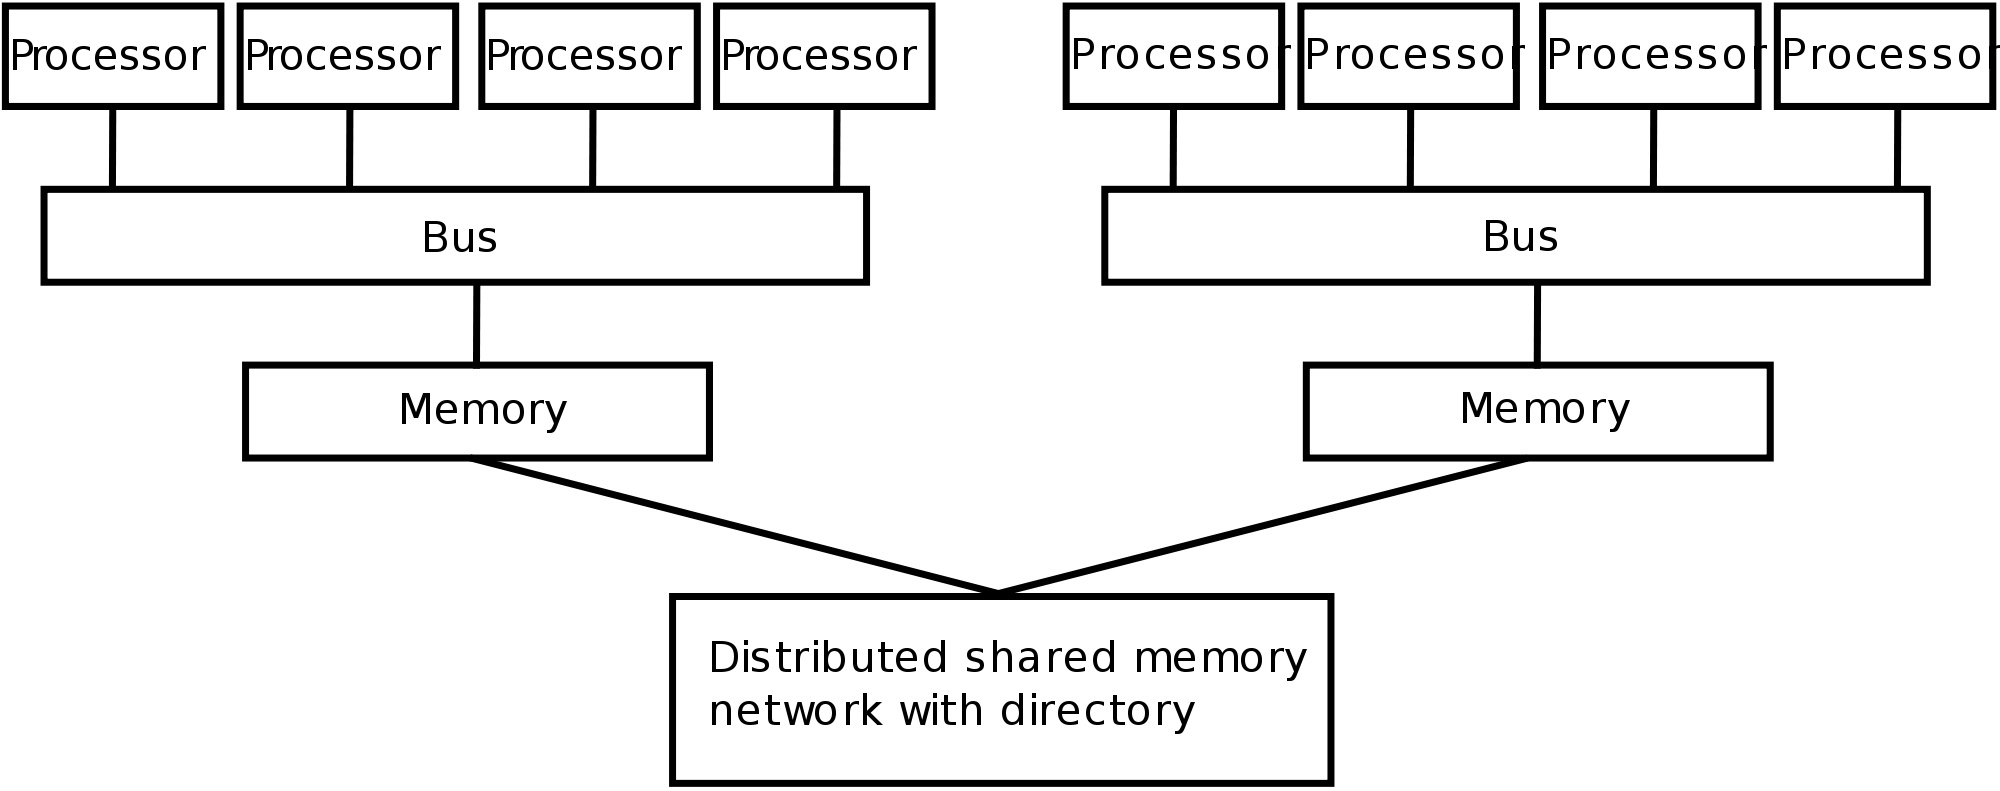
\includegraphics[width=\linewidth]{NumaScheme.png}	
	\caption{Simple scheme of a CC-NUMA architecture composed by two NUMA nodes.}
	\label{fig:sgiLoad}
\end{center}
\end{figure}

\subsection{Multicomputer Architectures}
A Multicomputer is a system composed by a range of possibly heterogeneous computers.
Each node in a multicomputer consists of one or a few CPUs, some RAM (conceivably shared among the CPUs at that node only), a disk and/or other I/O devices, and a communication processor. 
The communication processors are connected by a high-speed interconnection network. 
What all multicomputers have in common is that when an application program executes the send primitive, the communication processor is notified and transmits a block of user data to the destination machine (possibly after first asking for and getting permission).

The \textit{de facto} standard for interprocess communication in HPC environment is the MPI \textit{Message Passing Interface} library \cite{MPI}.
MPI has been implemented and optimized for a wide variety of systems and interconnect hardwares.


In the following we introduce the two computational systems used in this work.



\subsection{SGI ALTIX UV-2000 CC-NUMA}\label{numaarch:sec}

The CC-NUMA system we used is an SGI Altix UV2000 machine.
This machine is composed by four blades, each containing two NUMA nodes (e.g. one CPU 8-cores chip-set with one 128 GB local memory bank per node). 
Each node has to be considered as an extension of the motherboard, thus appearing as an unique machine to the operative system, with an unique memory address space.

\subsubsection{UV-2000 specifications}

\begin{itemize}
\item \textbf{Vendor}: SGI
\item \textbf{Nodes}: 8
\item \textbf{Blades}: 4
\item \textbf{Processors}: 1 8-cores Intel Haswell 3.3 GHz per node
\item \textbf{Cores}: 8 cores/node, 64 cores in total
\item \textbf{RAM}: 128 GB/node, 8 GB/core, total 1024 GB.
\item \textbf{Interconnect}: NUMAlink UVHub 3.0 (48 NUMAlink Ports)
\item \textbf{Disk Space}: 1.000 TB
\item \textbf{Operating system}: CentOS 7.0
\item \textbf{Batch system}: None. Direct access to the operative system.
\item \textbf{Serial Number}: UV2-00000510
\end{itemize}

Cpu specifications:

\begin{itemize}
\item \textbf{Vendor}: Intel
\item \textbf{Processor Number}: Xeon E5-4627 v2
\item \textbf{L3 shared cache size}: 16MB
\item \textbf{Instruction set}: 64-bit
\item \textbf{Max frequency}: 3.3 GHz
\item \textbf{Hyper-threading}: No 
\end{itemize}


\subsubsection{NUMAlink and GRU-MPT}
As said in section \ref{sec:multiprocessor} the main feature of multiprocessor architectures is the presence of shared memory.
In this framework the implementation of a program can be definitely easier compared with the need to use MPI libraries, but \QE has abandoned a shared memory design long time ago, being now strongly based on message massing directives.

To obviate this kind of problem, SGI provides the user with his own implementation of the MPI library, the so-called MPT\cite{MPT} \textit{Message Passing Toolkit library}.

This library gives the user the possibility to leverage the features of shared memory without the need to change their MPI-based code. 

We can see the MPT library as a shared memory wrapper for MPI calls. \footnote{The capabilities of the MPT toolkit goes wildly over the mere wrapping of MPI calls, but, in the scope of this work, this description is sufficient.}
The linux kernel module responsible for the operation of shared memory wrapping and intercommunication is called GRU.

In this framework all the work of intercommunication is demanded to the NUMAlink interconnect, which basically migrates and duplicates pages of memory to minimize local reference misses.

%For tuning parameters of MPT please refer to section XXX.

\subsubsection{Useful commands}\label{sec:UsefulCommands}
On the UV2000 a set of useful commands can be used to characterize the architecture.

We report the command name and a brief description.

\paragraph{cpumap} prints information on CPU locations and characteristics within the machine.

Sample Output: 
\lstinputlisting[basicstyle=\tiny ,breaklines=true,tabsize=2]{media/listings/cpumap.out}

We can see that the L3 cache is shared within the same node, composed by a single eight cores chip-set.


\paragraph{numactl} is a linux tool for general configuration of every NUMA architecture.
It can be used to print general information on memory usage and interconnect ``\textit{distances}".

Output:

\lstinputlisting[basicstyle=\tiny ,breaklines=true,tabsize=2]{media/listings/numactl.out}


We can see from the last lines of the output that nodes within the same blade are slightly ``\textit{closer}" than nodes on different blades, but the ``\textit{distance}" between two different blades is the same.

This should be considered just as a rough estimate of communication latency between the nodes.

\paragraph{topology} command prints in depth information on nodes location and CPU characteristics.

Output:
\lstinputlisting[basicstyle=\tiny ,breaklines=true,tabsize=2]{media/listings/topology.out}
From which we can also see the size of L1, L2 and L3 caches.


\subsection{IBM NetXScale CINECA ``Galileo" Cluster Architecture}\label{galileoarch:sec}

The multicomputer system we had the opportunity to use is the Galileo Tier-1 cluster hosted by CINECA \cite{Galileo}.

This supercomputer is among  the fastest supercomputer available to Italian industrial and public researchers. It is equipped with up-to date Intel accelerators (Intel Phi 7120p), NVIDIA accelerators (NVIDIA Tesla K80), as well as top level programming environment and a number of Application Tools required by the projects activated on it.

Galileo is mainly used to develop and run applications targeted at hybrid architectures, leveraging software applications in the fields of computational fluid dynamics, material and life science, and geophysics. The computing system is also available to European researchers as a Tier-1 system of the PRACE infrastructure.


\subsubsection{Galileo Specifications}

Cluster specifications: 
\begin{itemize}
\item \textbf{Vendor}: IBM Lenovo
\item \textbf{Nodes}: 516 
\item \textbf{Processors}: 2 8-cores Intel Haswell 2.40 GHz per node
\item \textbf{Cores}: 16 cores/node, 8256 cores in total
\item \textbf{RAM}: 128 GB/node, 8 GB/core
\item \textbf{Interconnect}: Infiniband with 4x QDR switches
\item \textbf{Disk Space}: 2.000 TB of local scratch
\item \textbf{Operating system}: CentOS 7.0
\item \textbf{Batch system}: PBS Pro (Topology-aware)
\end{itemize}

Cpu specifications:
\begin{itemize}
\item \textbf{Vendor}: Intel
\item \textbf{Processor Number}: Xeon E5-2630V3
\item \textbf{L3 shared cache size}: 20MB
\item \textbf{Instruction set}: 64-bit
\item \textbf{Max frequency}: 3.2 GHz
\item \textbf{Hyper-threading}: No 
\end{itemize}



\subsection{Bias Factors}

There are a number of factors that can impact on the performances of a \QE simulation on both the systems.

\subsubsection{Libraries and compilers}

As specified in section \ref{sec:QE}, \QE is implemented using different libraries. 
Besides the FFTW\cite{FFTW}, which is distributed within the \QE package, the libraries for linear algebra (BLAS\cite{BLAS}, LAPACK\cite{LAPACK}, ScaLAPACK\cite{SCALAPACK}) and communication (MPI\cite{MPI},OpenMP\cite{OMP}) are all external.

A wide variety of implementation of those libraries exists each of these can be compiled with different compilers.
There are two popular compilers used by \QE community: GNU compilers and Intel compilers \footnote{\QE is implemented using different languages (fortran, C, C++,...) }.

We performed a simple test on Galileo using both the compilers on the Cobalt(II,III)oxide system( \CO, see appendix \ref{app:Co3}). 
We measure the execution time\footnote{See section \ref{sec:Metrics}.} of the PWscf package compiled with different configurations: 
\begin{itemize}
	\item \textbf{GNU} : GNU compiler suite v4.9.2, OpenMPI v1.8.4, FFTW v3.3.4, BLAS v3.5.0, SCALAPACK 2.0.2\footnote{ All the libraries were compiled using the GNU suite.}.
	\item \textbf{INTEL} : Intel CS XE 2015 compiler suite, IntelMPI v5.0.2,  FFTW v3.3.4, MKL v11.2
%	\item \textbf{GNU and MKL}  : same configuration as in the \textbf{GNU} configuration but linking against the Intel MKL package for liner algebra.
\end{itemize}
The result are exposed in table \ref{tab:libraries}.

\begin{table}[h]
\centering
\begin{tabular}{lcc}
\textbf{cores} & \multicolumn{1}{l}{\textbf{GNU}}  & \multicolumn{1}{l}{\textbf{INTEL}} \\ \hline \hline
\textbf{1}     & 1h 52m                            & 22m 57s                            \\
\textbf{64}    & 6m 3s                            		& 1m 50s                            
\end{tabular}
\caption{Execution time for PWscf runs on CO3 system with different compilers and libraries.}
\label{tab:libraries}
\end{table}

%\begin{table}[h]
%\centering
%\begin{tabular}{lccc}
%\textbf{cores} & \multicolumn{1}{l}{\textbf{GNU}} & \multicolumn{1}{l}{\textbf{GNU+ItelMKL}} & \multicolumn{1}{l}{\textbf{INTEL}} \\ \hline \hline
%\textbf{1}     & 1h 52m                           & 1h 50m                                   & 22m 57s                            \\
%\textbf{64}    & 6m 3s                            & 5m 58s                                   & 1m 50s                            
%\end{tabular}
%\caption{Execution time for PWscf runs on CO3 system with different compilers and libraries.}
%\label{tab:libraries}
%\end{table}


We can see that the native Intel compilation is considerably more efficient than the open-source alternatives.

The results at one core highlight that the big difference must lie in how FFT and linear algebra is performed by the two solutions. 

%The use of MKL library seems to have little effect on the overall result, but one must consider that for such a system the great computational complexity lies in the FFT performance. section XXX.}

\begin{framed}
For this reason all the tests we have done were performed using ``\textit{state of the art}" compilers and libraries available on each architecture.
\end{framed}


\subsubsection{Node Load}

In modern HPC computing is common to share resources. Big multicomputers clusters are often used by thousands of users simultaneously.
In this framework, if the amount of CPUs required by the task is less than the total number of CPUs available on the node, it is almost certain that the remaining CPUs will be occupied by other users' computations.
As a consequence the L3 cache is divided among different uncoherent processes, as one can imagine the impact on performance cannot be beneficial.

To estimate the effect of resource sharing on \QE simulations we performed a set of tests on the \CO  system. 


On Galileo cluster the results are reported in table \ref{tab:galileoNodeLoad}.

\begin{table}[hhh!]
\centering
\begin{tabular}{r|cc}
\textbf{cores} & \textbf{reserved} & \textbf{shared} \\ \hline \hline
1              & 22m 57s           & 32m 51s         \\ % 70\% resever/shared
2              & 12m 15s           & 16m 58s         \\ % 72\%
4              & 7m 16s            & 8m 52s          \\ % 83\%
8              & 4m 1s             & 4m 25s             % 91\%
\end{tabular}
\caption{Execution time for the \CO system on totally reserved and shared nodes.}
\label{tab:galileoNodeLoad}
\end{table}

It is clear that sharing resources has an impact on the execution time. 
The difference decreases when the number of CPUs rises. 
Unfortunately it is not possible to select the exact CPUs to occupy, thus we cannot see if reserving the first eight CPUs\footnote{Being on the same CPU-set, they share the same L3 cache.} belonging to the same chip-set would lead to the same result than on shared nodes.

On the UV2000 we had the possibility to perform more extensive tests and the results are reported in figure \ref{fig:sgiLoad}.


\begin{figure}[hhh!]
\begin{center}
	\captionsetup{justification=centering}
	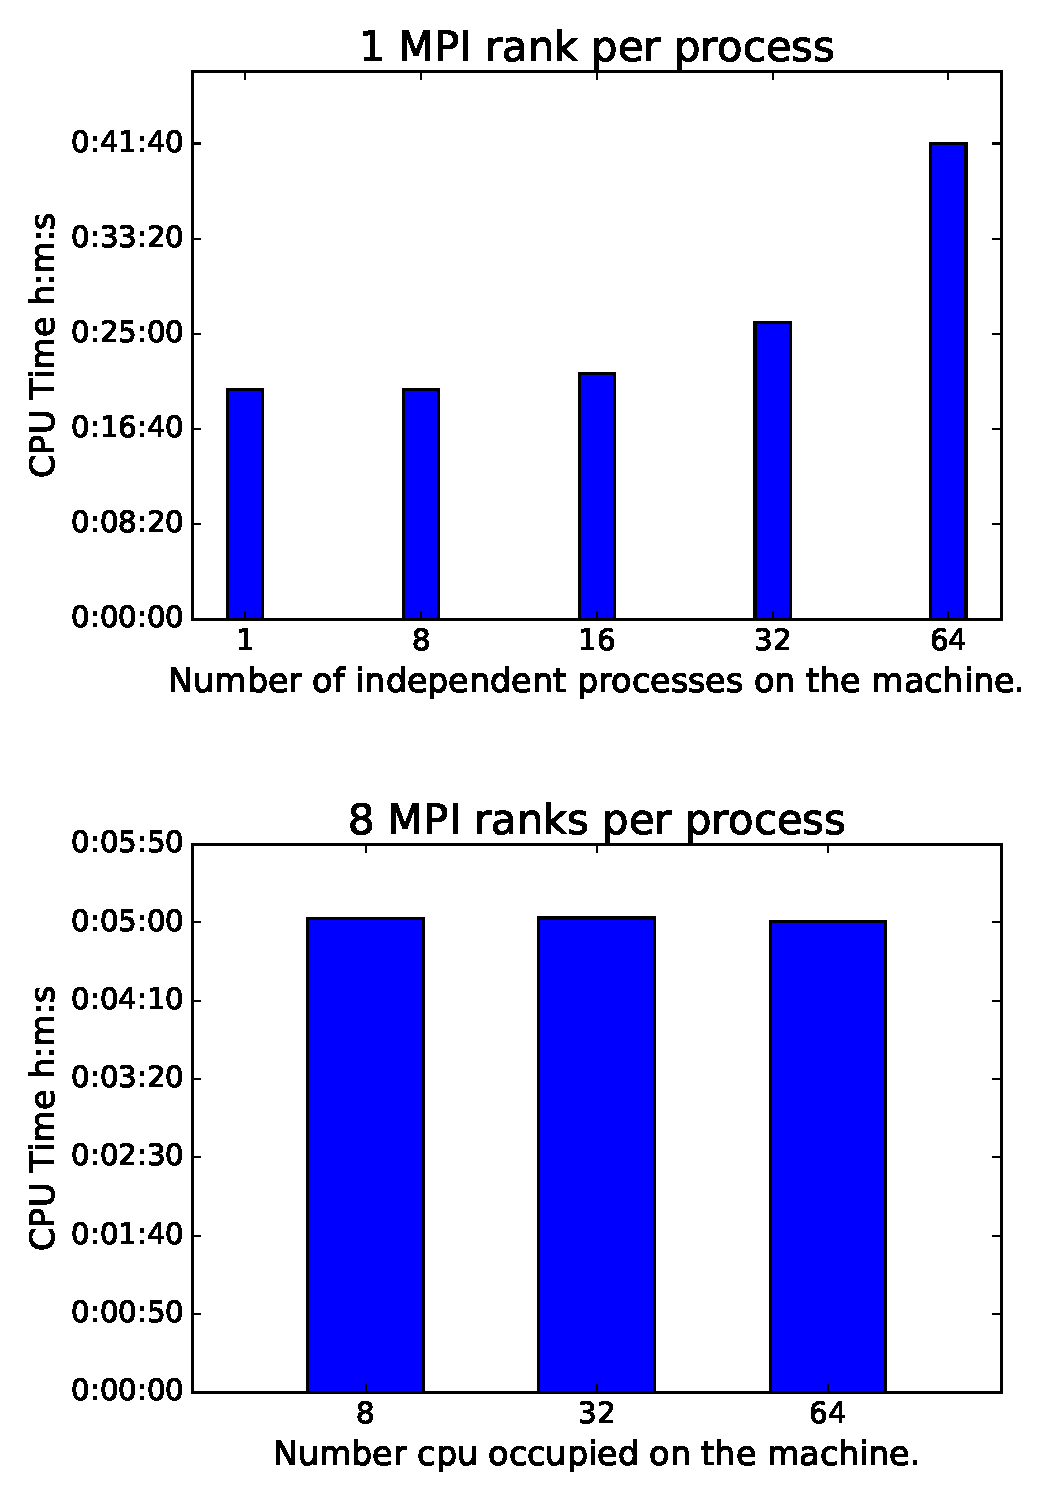
\includegraphics[width=0.7\linewidth]{sgiLoad.pdf}	
	\caption{First plot: execution time of independent 1 rank PWscf process in function of the number of independent processes simultaneously running on the machine. 
	\\Second Plot: execution time of independent 8 rank processes in function of the number of occupied processor on the machine.}
	\label{fig:sgiLoad}
\end{center}
\end{figure}

To simulate different load conditions we ran simultaneously different instances of PWscf performing the same calculation\footnote{Of the \CO system.}. Each instance of PWscf is completely independent.

In the first graph each instances was composed by a single MPI process, without threads. 
The execution time is plotted in function of the total number of independent processes running simultaneously on the machine.
The processes were equivalently spaced among the CPUs\footnote{Except for the first bar, the load of each node was the same.}.

Two aspects can be clearly seen.

First, the execution time rises after 16 cores are simultaneously occupied (at least half of the cores on each node).
When all the CPUs are occupied the execution time is more than doubled. 
We can say that the UV2000 performs poorly compared to the traditional cluster when multiple independent tasks have to be performed at the same time.

The second observation is that the execution time of the first and second bars are very close. 
In the first bar only a single CPU for on the whole machine is used; in the second bar a single CPU (the first one) for each node is used;
The fact that the times are the same suggests that each node behaves almost independently.

To confirm this speculation we raised the number of MPI ranks per PWscf instance to eight\footnote{The number of CPUs in a node.} and we performed three tests represented  in the second graph of figure \ref{fig:sgiLoad}.
The first bar occupies only one node per machine, the second occupies half of the nodes and the third all of the nodes.

The execution times are basically the same, our hypothesis is confirmed:

\begin{center}
\begin{framed}
\textit{the UV2000 machine can be used to perform simultaneously different independent calculations, provided that each node (or set of nodes), is dedicated to the same task.}
\end{framed}
\end{center}

The same results can be obtained with different numbers of MPI ranks per instance.

\begin{framed}
After these preliminary tests, we decided to run every calculation reserving the whole resource, being it a Galileo node or the whole UV2000 machine.
\end{framed}

To see how it's possible to reserve an entire Galileo node refer to appendix \ref{app:PBS}

\subsubsection{Process migration (UV2000)}

In modern multiprocessor architecture, even in a common desktop workstations, the Linux scheduler is used to migrate active processes from one CPU to another. 
In machines with a single shared memory controller  or with multiple controllers with uniform memory access time \footnote{UMA \textit{Uniform Memory Access} machines.}, the migration of a process doesn't have an impact on performances.
On NUMA machines instead, where the time to access a memory page depends on the page location within the machine topology, this could negatively influence the performance of the code.
On the UV2000, memory allocation requested by a process is performed on the same node the process is running on. 
If the process is then migrated to another node the memory access time will increase roughly by a factor of five.\footnote{See section \ref{sec:UsefulCommands}.}
The impact is mitigated by the NUMAlink behavior, which will migrate memory pages closer to the new process location (if available).

Another effect one must consider is that if an MPI job is launched on a subset of cores, i.e. requesting eight ranks, the ranks are randomly spread trough the whole machine.
Making a simple analogy, it would be equivalent to launch eight MPI processes each on a different Galileo node and expect the same performances.
If we introduce threads the scenario can get increasingly more complicated.
To obviate this problem SGI developed a set of three utilities: \texttt{omplace}, \texttt{nodeinfo} and \texttt{dlook}.

\paragraph{omplace:} \texttt{omplace} is a command that forces the scheduler to maintain a process on the selected core, this feature is called \textit{process pinning}. 
\texttt{omplace} automatically takes care of threads placement and provides great flexibility on CPU selection.
In order to use \texttt{omplace} it is sufficient to prepend it to the executable call, just after the \texttt{mpirun} call.

For example:
\begin{verbatim}
	mpirun -np 8 	omplace -c 0-7 pw.x
\end{verbatim}
will launch eight MPI ranks on the first eight processors.

In case threads are used :
\begin{verbatim}
	export OMP_NUM_THREADS=4
	mpirun -np 2 omplace -c 0-7 pw.x	
\end{verbatim}
they would be placed as follows\footnote{See \texttt{man omplace}.}
\begin{verbatim}
    rank 0 thread 0 on CPU 0
    rank 0 thread 1 on CPU 1
    rank 0 thread 2 on CPU 2
    rank 0 thread 3 on CPU 3
    rank 1 thread 0 on CPU 4
    rank 1 thread 1 on CPU 5
    rank 1 thread 2 on CPU 6
    rank 1 thread 3 on CPU 7
\end{verbatim}

Although \texttt{omplace} can be used also with openMPI implementations, it has proven to be reliable only with MPT
\footnote{\texttt{taskset} and \texttt{dplace} are two other tools to provide process pinning, but during our preliminary test they did not appear to be reliable.}.

\paragraph{nodeinfo:}\texttt{nodeinfo} is a monitoring program that provides real time statistics on memory usage.

The per-node information provided are:
\begin{itemize}
	\item Free and used memory.
	\item Memory allocated on the node by local processes.
	\item Memory allocated on the node by non-local processes.
	\item Memory allocated on non-local nodes by local processes.
\end{itemize}

Using these metrics one can evaluate if a program is managing poorly the memory allocation.

\paragraph{dlook:} \texttt{dlook} program gives in-depth information on memory allocation regarding a specific process.
\texttt{dlook} lists all the pages allocated by the program along with their memory address and node location.

A sample of \texttt{dlook} output for a PWscf process follows:
\lstinputlisting[basicstyle=\tiny ,breaklines=true,tabsize=2]{media/listings/dlook.out}


We used \texttt{dlook} and \texttt{nodeinfo} to evaluate if the memory allocation performed by \QE adapts properly to the NUMA architecture.

The results have highlighted a very rational way of allocating memory.
For instance, memory structures that are local to the single MPI rank are allocated within the rank and not allocated outside the rank and then passed with \texttt{send/recv} directives.
This is a consequence of the design of \QE that makes wide use of all-to-all MPI directives, which are efficiently implemented by MPT.
Thus \QE seems to adapt well to the NUMA environment.

\begin{framed}
	Every run on the UV2000 machine is performed using the \texttt{omplace} utility to ensure a correct process pinning and avoid overhead in memory allocation and/or communication.
\end{framed}



\subsection{Profiling tools}\label{sec:profTools}

To evaluate the performance of the subroutines in \QE we mainly used two tools.

\paragraph{Internal PWscf metrics:} when PWscf successfully completes a run, an extensive set of metrics is printed\footnote{On the stdout or the specified output file.}. 
For each of the main subroutines  \textit{cpu time}, \textit{wall time} and the number of calls are reported.
See section \ref{sec:Metrics} for further detail on metrics values.

\paragraph{Scorep code instrumenter:} \texttt{scorep}\cite{SCOREPManual} is a code instrumenter developed by the VI-HPS institute \cite{VH}. 
A code instrumenter is a compiler wrapper able to ``\textit{instrument}" each function call inside source files.
Namely, the time the subroutine is invoked and the time it exists are automatically stored.
One of the great advantages of \texttt{scorep} is that it's a full \textit{in-memory instrumenter}, meaning that all the metrics computed are stored into the system RAM memory and are written to the disk only when the run is completed.
This feature reduces drastically the runtime overhead during profiling runs, making thus possible to profile complex programs having tens of millions of function calls ( this is literally the case for \texttt{h\_psi}).
Runtime overhead on the UV2000 is of the order of $25\%$ while on Galileo it could reach $50\%$; a remarkable result compared to \texttt{gprof}.

In order to use \texttt{scorep} it is sufficient to recompile \QE prepending the \texttt{scorep} command to every compiler invocation and  \texttt{scorep}'s libraries must be used during linking time; see section \ref{sec:ConfSummary} for more details on \QE compilation.

To profile the code it is sufficient to run the PWscf executable compiled in the step above, this produces a ``\textit{profile.cubex}" binary file with an incredibly small disk footprint\footnote{For a run on 64 cores of a 160 atom system with 70 scf iterations the result file is around 20MB.}.
The ``\textit{profile.cubex}" file can be inspected using the ``\textit{cube}" gui program, which is distributed together with \texttt{scorep}. As an alternative one can also use the ``\textit{paraprof}" suite.

The metrics produced by these tools are compatible.\footnote{ Obviously after rescaling \texttt{scorep}'s metrics by the total overhead factor.}

In this work we were able to obtain most of the useful information from internal PWscf's metrics, nevertheless \texttt{scorep} was used for in-depth analysis of the call graph and to compute the percentage time spent during MPI communication.

\paragraph{Developed tools:} I have developed a set of python scripts in order to analyze and plot internal metrics with a certain flexibility. The complete source code can be found at \cite{qetools}.


\subsection{Metrics}\label{sec:Metrics}

In this section we outline the metrics used to measure PWscf performances on both architectures.

\subsubsection{Direct Metrics}\label{sec:DirectMetrics}
Two are the main metrics directly produced by the tools listed in section \ref{sec:profTools}.

\paragraph{CPU time: } CPU time (or process time) is the amount of time for which a CPU was used for processing instructions of a computer program. CPU time does not include time in which the program was stopped by the scheduler or time spent during I/O operations. \footnote{Typically in UNIX and UNIX-like systems I/O operations are always performed using of system calls. System calls can be blocking or not-blocking but they don't contribute to CPU time.}

\paragraph{WALL time: } WALL time (or wall-clock time) is the human perception of the passage of time from the start to the completion of a task. 
In the context of a task being performed on a computer, wall-clock time is a measure of the real time that elapses from start to end, including time that passes due to programmed (artificial) delays or waiting for resources to become available (I/O operations). 
In other words, it is the difference between the time at which a task finishes and the time at which the task started.

If not explicitly specified, all considerations contained in this work refers to CPU time.

To minimize the amount of I/O operations performed by PWscf we set the PW control variable \texttt{disk\_io} to \texttt{`none'}\cite{PWinput}.
This reduces the amount of I/O operations to the bare minimum.

In figure \ref{fig:cpuwalltime} we can see that the difference between the two metrics is negligible for all the subroutines.\footnote{Note that the resource was fully reserved and no other system processes were running.}

Consider also that \QE does not utilize the MPI distributed I/O directives.

\begin{figure}[hhh!]
\begin{center}
	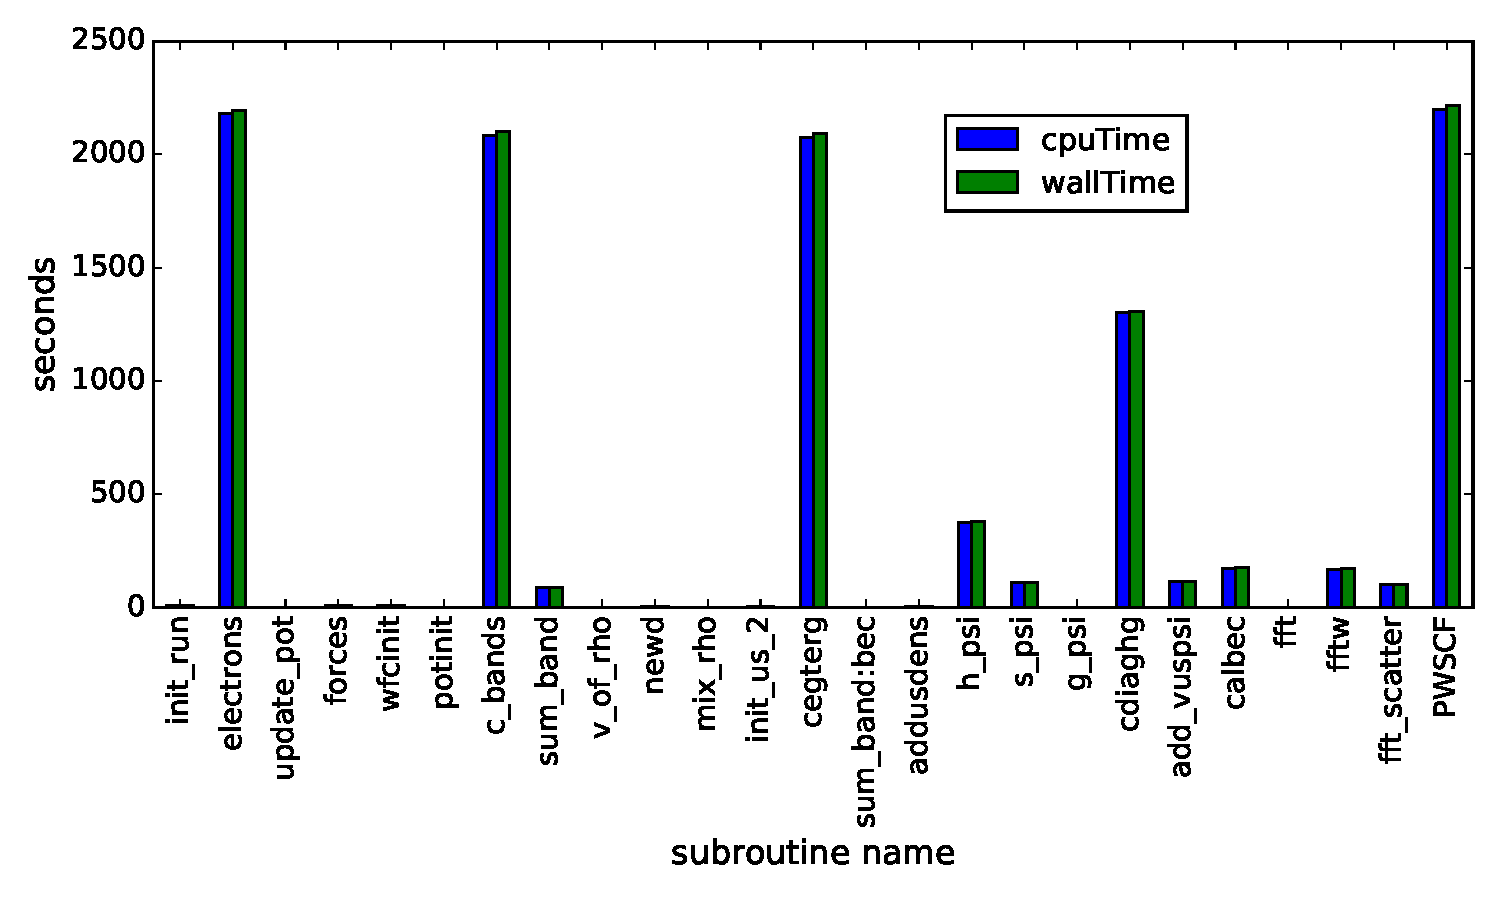
\includegraphics[width=\linewidth ,height=10cm]{cpuwalltime.pdf}	
	\caption{CPU time and WALL time with \texttt{disk\_io = `none'} for a 164 atom system scf calculation.}
	\label{fig:cpuwalltime}
\end{center}
\end{figure}

\subsubsection{Indirect Metrics}

The following metric is an indirect metric that can be obtained from the previous two.

\paragraph{speedup:}  CPU time can be used to compare different runs of PWscf performed on the same architecture\footnote{Fortunately Galileo is a completely homogeneous cluster.}, but if one want to compare different architectures an a-dimensional metric is needed.

We introduce the ``\textit{speedup}" as defined in \cite{Tanenbaum} : 
\begin{equation}\label{eq:speedup}
	s = \frac{T_{1}}{T_{N}},
\end{equation}
where $T_{1}$ is the runtime (CPU time in our case) of the program on a single core (i.e. the serial execution of the program), while $T_{N}$ is the execution of the program performed in parallel using $N$ cores.
Hence the speedup is ``\textit{how much faster the programs are going to run on a parallel computer than on a
uniprocessor}"\cite[p.648]{Tanenbaum}.

\begin{figure}[hhh!]
\begin{center}
	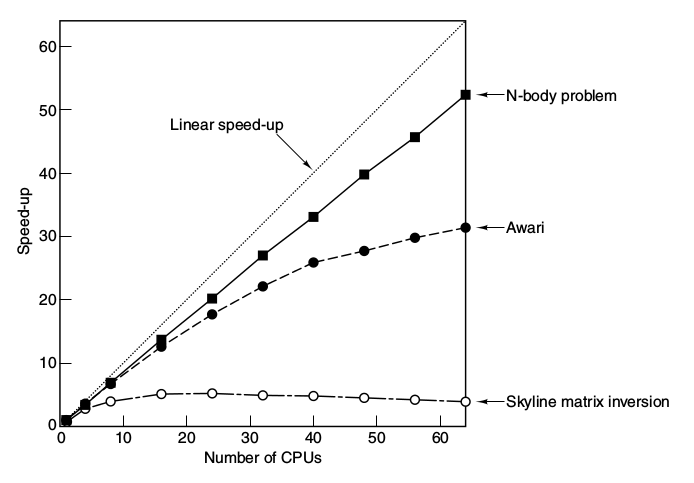
\includegraphics[scale=0.5]{tanenbaum_speedup.png}	
	\caption{Speedup of three different algorithms \cite{Tanenbaum}.}
	\label{fig:TanenbaumSpeedup}
\end{center}
\end{figure}

Speedup tels us ``\textit{how good a program scales on a defined architecture}", then it provides an useful metric to compare different computational architectures.

Speedup is also used to compare performances of different programs\footnote{Or different inputs of the same program.} on the same machine.



An illustration taken directly from \cite{Tanenbaum} is reported in figure \ref{fig:TanenbaumSpeedup}.
As we can see the ideal linear speedup cannot be reached by real programs, this happens because some of the components of the program would always be serial\footnote{For example any \textit{reduce} MPI call is executed on a single MPI rank.}.

\subsection{Configuration summary}\label{sec:ConfSummary}

The version of \QE used on both the systems was v5.2.1.

Full threaded version of MKL and SCALAPACK implementations optimized for each architecture have been used.

In appendix \ref{app:makefiles} the complete makefiles of \QE are reported.

To summarize the configuration used for all the tests:
\begin{itemize}
	\item We used compilers and libraries at the ``\textit{state of the art}" available on each architecture.
	\item We reserved the whole computational resource, being it a Galileo node or the whole UV2000 machine.
	\item Every run on the UV2000 machine is performed using the \texttt{omplace} utility to ensure a correct process pinning and avoid overhead in memory allocation and/or communication.
	\item The PWscf's parameter \texttt{disk\_io} was set to `\texttt{none}' to minimize I/O operations and avoid differences between CPU time and WALL time.
\end{itemize}

\newpage




\section{Results}\label{sec:results}
This section consists of a very deep insight into all the components of the PWscf package and their interaction with the computational architecture used.

Therefore, what follows can be considered as a very technical section, both for the tools used and the observations made.

Nevertheless we will try to expose the results from two points of views :
\begin{itemize}
	\item a technical point of view, focused on the factors that can improve the performance of each PWscf's component;
	\item a pragmatic point of view, focused on the factors that can improve the performance of the overall simulation.
\end{itemize}
Although at first the distinction can seem subtle, it will be clear in the following that a great difference exists between them.

We remind the reader that each PWscf run is performed following the directives outlined in section \ref{sec:ConfSummary}.

If not reported explicitly, all the time metrics exposed have to be considered as CPU time, see section \ref{sec:DirectMetrics} for further details.

\newpage

\subsection{Goals}\label{sec:Goals}
We found appropriate to divide the results we obtained in three main categories.

\paragraph{Highlight of critical components} 
In section \ref{sec:resCriticalComponents} we will perform an in-depth analysis of what are the most important components of PWscf.

We aim to find an answer to the following questions :
\begin{itemize}
	\item What are the most computational intensive subroutines and what kind of calculation is performed?
	\item Where the interprocess communication happens and what are the main MPI subroutines used? Is it possible to have a rough estimate of the weight of communication over computation?
	\item What is the dynamic of the SCF iteration? 	
\end{itemize}

This section will highlight what components should be considered while profiling PWscf and what are the critical behaviors of the code. 
Therefore it serves as an important introduction to section \ref{sec:resArchIndependent} and \ref{sec:resArchDependent}. The difference between the two points of view exposed in section \ref{sec:results} will be cleared here.



\paragraph{Architecture Independent Tuning}
In section \ref{sec:resArchIndependent} we'll focus on the factors that can improve PWscf's performance regardless of the memory access architecture.

We focused mainly on the effects of second level thread parallelization because it is the easiest way to alter the behavior of PWscf without the need to tune complex runtime parameters.

Hence the question we want to answer:
\begin{itemize}
	\item What is the overall impact of thread parallelization?
	\item What is the impact of thread parallelization on each component?
	\item In which scenario is convenient to use thread parallelization?
\end{itemize}

This section will give all the tools necessary to tune the performance of the code in a workstation-scale environment, very familiar to researchers of the field.

\paragraph{Architecture Dependent Tuning}
Finally, in section \ref{sec:resArchDependent} we will make an in-depth investigation on the performance of the two computation architecture exposed in section \ref{sec:comparch}.

What we aim to know is :
\begin{itemize}
	\item What is the overall performance on each architecture?
	\item What are the components that performs best on each architecture?
	\item What architecture has the best implementation of interprocess communication?
	\item How diagonalization distribution impacts PWscf performance on both architectures?
	\item What is the overall behavior of \QE in function of the scale of the physical system?
\end{itemize}

This section will underline the differences between the two architectures and propose a simple method to enhance PWscf performance on both of them.

\newpage

\subsection{Titanium Dioxide}\label{sec:titania}

Titanium dioxide (TiO\textsubscript{2} or  Titania) has been the subject of extensive research in recent years due to its relevant photochemical and photophysical properties combined with its natural abundance, low cost, and superior chemical and photostability \cite{Titania1},\cite{Titania3}. 

Titanium dioxide is used in heterogeneous catalysis, as a photocatalyst, in solar cells for the production of hydrogen and electric energy, as gas sensor, as white pigment (e.g. in paints and cosmetic products), as a corrosion-protective coating, as an optical coating, in ceramics, and in electric devices such as varistors. 

It is important in earth sciences, plays a role in the biocompatibility of bone implants, is being discussed as a gate insulator for the new generation of MOSFETS and as a spacer material in magnetic spin-valve systems, and finds applications in nanostructured form in Li-based batteries and electrochromic devices \cite{Titania2},\cite{Titania4},\cite{Titania5}.

For these reasons, in this work we focused on the study of \QE performance when simulating Titanium dioxide  materials in nanocrystalline form.

The supercells hosts a surface of TiO\textsubscript{2} in which proximity is present an H\textsubscript{2} molecule.
To simulate the surface configuration it is necessary to extend the supercell on the z axis leaving a wide portion of the cell empty.

Note that in this way the number of plane waves needed to approximate empty regions of space increases significantly, both because the cell is bigger (see section \ref{sec:FFT}) and because the Kohn-Sham orbitals must be null if no electron is expected to be found, implying an higher number of Fourier's coefficients to null the state function.

The system is composed by 54 Titania atoms, 108 Oxygen atoms and 2 atoms of Hydrogen for a total of 2054 electrons; 
The full specification of PWscf input file can be fund in appendix \ref{app:titania}. 
A rendering of the system is represented in figure \ref{fig:titania}.

This kind of system was chosen as a representative sample of all the possible configurations that can be studied, it is also compelling for molecular dynamic simulations, where a great number of sequenced SCF iterations have to be performed.

\begin{figure}[hhh!]

\centerline{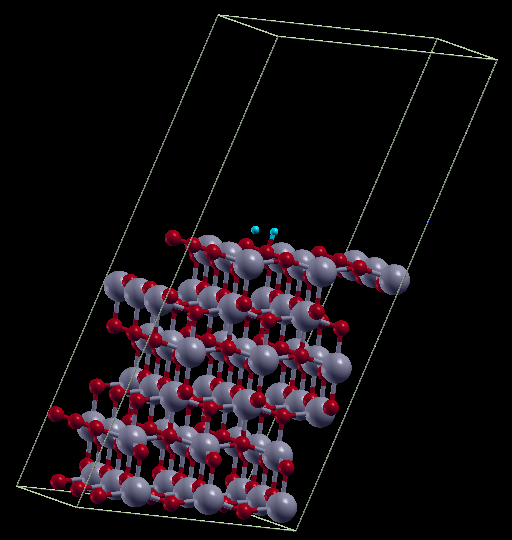
\includegraphics[scale=0.5]{titania_crystal.png}}
	\caption{Test system: TiO\textsubscript{2} surface with an H\textsubscript{2} molecule in proximity.}
	\label{fig:titania}

\end{figure}

\newpage

~

\newpage
\subsection{Highlight of critical components}\label{sec:resCriticalComponents}

\begin{center}
\begin{framed}
What are the most computational intensive subroutines and what kind of calculation is performed?
\end{framed}
\end{center}

\begin{figure}[hhh!]
\begin{center}
	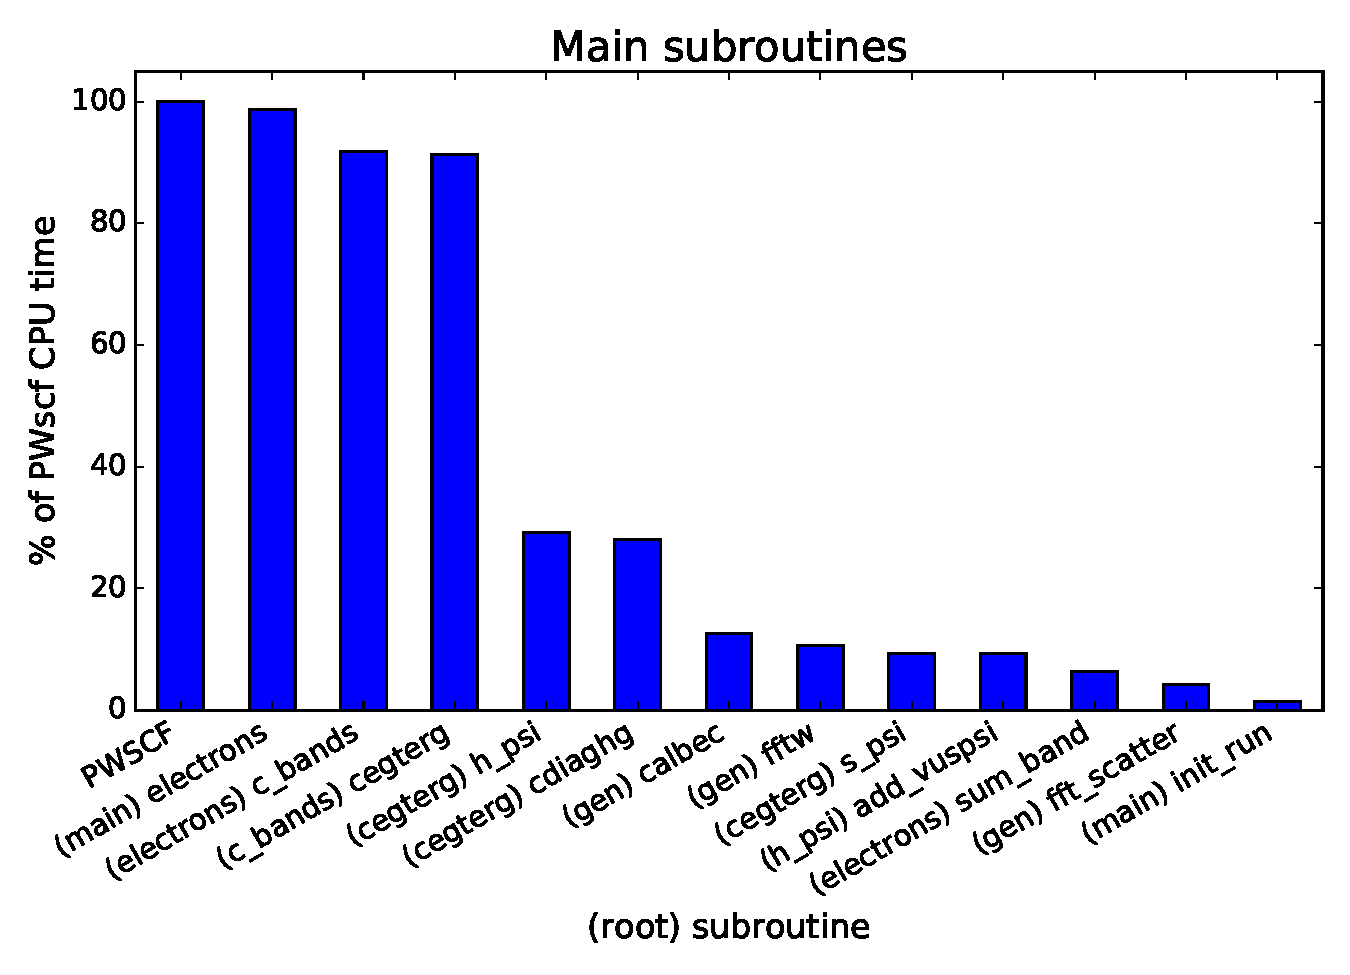
\includegraphics[width=\linewidth]{main_subroutines.pdf}	
	\caption{Percentage of total PWscf CPU time per routine sorted by descending value. 
	\\In parenthesis the caller(root) subroutine is reported. 
	Subroutines with the same caller are plotted with the same color. 	
	\\``gen" refers to subroutines belonging to external \QE modules, hence called in different subroutines. }
	\label{fig:mainSubroutines}
\end{center}
\end{figure}

In figure \ref{fig:mainSubroutines} we have plotted the subroutines consuming the most CPU time. 
The data were obtained from a run at 4 MPI ranks, to have an average indication of the behavior of the code.

The CPU time of the single subroutine is compared to the CPU time of the whole PWscf's run in form of percentage.
This is an inclusive metric, meaning that the CPU time of each subroutine includes the CPU time spent in every subroutine called.
We have color-coded the subroutines that are called by the same caller.

We remind the reader that an analysis of the operations performed by the most important subroutines can be found in section \ref{sec:QE}.


PWscf calls mainly two subroutines: \texttt{init\_run} and \texttt{electrons}.
Approximately 99\% of the total run time is occupied by \texttt{electrons}, which is the subroutine implementing the whole SCF iteration \footnote{Obviously if only one SCF step is performend the percentage would be different, remember also that 30 steps is a reasonable average for the number of iterations to reach self-consistency. }.

\texttt{Electrons} calls \texttt{c\_bands} to obtain the Kohn-Sham orbitals\footnote{The eigenvectors of $\mf{H}^{KS}$.} and \texttt{sum\_band} combines them to obtain the electronic density.

\texttt{C\_bands} is basically a wrapper for \texttt{c\_egterg}, which implements the Davidson diagonalization (see section \ref{sec:Diagonalization}), in fact it calls two functions:
\texttt{h\_psi} to evaluate the $\mf{H}^{KS}$ matrix and \texttt{cdiaghg} to diagonalize the obtained matrix.

\texttt{Fft\_scatter} is a subroutine that distribute Kohn-Sham orbitals values on the grid among all the MPI ranks, hence it is mainly dedicated to communication, while \texttt{fftw} is the routine that actually computes the FFT and IFFT transformations (see section \ref{sec:FFT}).

We can outline a list of the most important subroutines that we will keep under consideration in the followings:

\begin{center}
\texttt{cegterg, h\_psi, cdiaghg, sum\_band, fftw, fft\_scatter} \label{asd:relevantFunctions}
\end{center}

\texttt{Cegterg} will be used as an indicator of the behavior of the whole SCF iteration;
\texttt{h\_psi} and \texttt{cdiaghg} will tell us respectively how the evaluation and the diagonalization of the matrix performs, which are two completely different kind of calculations;
by comparing \texttt{fftw} and \texttt{fft\_scatter} we can obtain a rough estimate of the relative weight of computation against communication in function of the cores used; 
finally we expect \texttt{h\_psi} and \texttt{sum\_bands} to behave similarly because the calculation performed are very alike.





\newpage
\begin{center}
\begin{framed}
Where the interprocess communication happens and what are the main MPI subroutines used? 

Is it possible to have a rough estimate of the weight of communication over computation?
\end{framed}
\end{center}


\begin{figure}[hhh!]
	\centerline{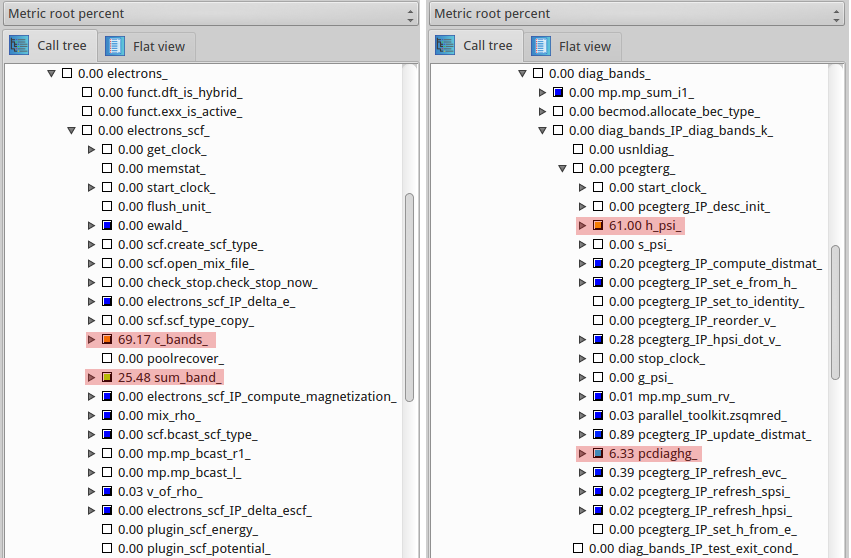
\includegraphics[scale=0.5]{cube_MPI.png}}
	\caption{Percentage of bytes sent/received per routine. The percentage is calculated against the total amount of bytes sent/received.  Tool: \texttt{cube} on \texttt{scorep}'s metrics.
	}
	\label{fig:cubeMPI}
\end{figure}

In figure \ref{fig:cubeMPI} we have two screenshots taken directly from \texttt{cube}, the \texttt{scorep} visualization tool (see section \ref{sec:profTools}).
The subroutines are represented in a call tree.

The number on the left of each subroutine is the percentage of bytes sent using MPI communication library inside the subroutine. 
The percentage is calculated over the total number of bytes sent in the whole execution, i.e. an absolute metric.
This is a cumulative metric between all the MPI ranks, hence the number of sent bytes and received bytes is the same.
Please note also that, as we will see below, the MPI subroutines used are very symmetric between the ranks, hence the cumulative metric is a valid way to measure the overall communication weight.

The color box on the left is an ``\textit{heat map}" representing the metric's value, blue is 0\% and red is 100\%\footnote{Since we are using absolute percentage values as metric, the color box is redundant. Nonetheless it can be incredibly useful when non-absolute metrics (metrics referring to the local root) are investigated.}.

On the left frame we explored the content of \texttt{electrons} and, as said above, we can see that \texttt{c\_bands} and \texttt{sum\_bands} are called.
It is clear that 69\% of the overall communication is performed to find the Kohn-Sham orbitals in \texttt{c\_bands}, this is expected since the evaluation of the matrix and its diagonalization is wildly parallelized.
Another 25\% of the communication is performed inside \texttt{sum\_band}, this important amount is due to the fact that \texttt{sum\_band} needs all the grid values of the eigenvectors obtained from the diagonalization to perform the final superposition and compute the electronic density.



In the right frame we explored \texttt{pcegterg}, which is the parallelized version of \texttt{cegterg}, containing the well known subroutines \texttt{h\_psi} and \texttt{p\_cdiaghg} (the ScaLAPACK parallelized version of \texttt{cdiaghg}).
It is evident that a significant amount of communication is performed by \texttt{h\_psi}, this is because an high number of distributed FFT and IFFT must be performed. On the contrary the distributed diagonalization has a lower impact on communication. 

Note that it was not possible to collect metrics on the communication performed inside each ScaLAPACK function\footnote{The communication part of the ScaLAPACK library is performed within the BLACS(Basic Linear Algebra Communication Subprograms) library.} because we would have to recompile the linear algebra libraries, which on both of the architectures are closed source.


\begin{figure}[hhh!]
	\centerline{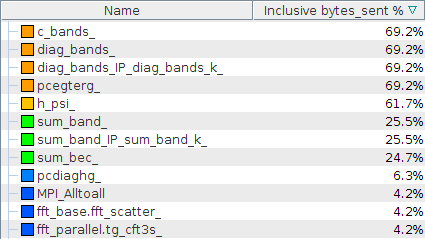
\includegraphics[scale=0.5]{mpi_inclusive_bytes_sent.png}}
	\caption{ Inclusive percentage of bytes sent/received by subroutines called inside \texttt{electrons}. The percentage is calculated over the total amount of bytes sent/received. Tool: \texttt{paraprof} on \texttt{scorep} metrics.
	}
	\label{fig:MPIinclusive}
\end{figure}

\begin{figure}[hhh!]
	\centerline{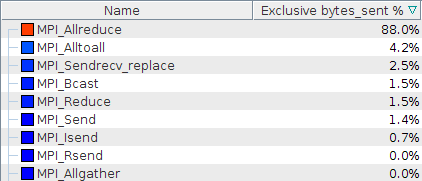
\includegraphics[scale=0.5]{mpi_exclusive_bytes_sent.png}}
	\caption{ Exclusive percentage of bytes sent/received by subroutines. 
	The percentage is calculated over the total amount of bytes sent/received. 
	As a result, the most important MPI subroutines are listed.
	Tool: \texttt{paraprof} on \texttt{scorep} metrics.
	}
	\label{fig:MPIexclusive}
\end{figure}

In figure \ref{fig:MPIinclusive} is reported an extract of the same data exposed in figure \ref{fig:cubeMPI} in a tabular view (also called a ``\textit{flat}" view).

In figure \ref{fig:MPIexclusive} the metrics reported is the same but is computed as an exclusive metric: for each root subroutine the metrics (bytes in this case) produced by inner subroutines are not considered.

As a result only the final communication subroutines (MPI, in this case) have non-zero amount of sent/received bytes.

We can clearly see that 88\% of the bytes sent/received are exchanged using the \texttt{MPI\_Allreduce} subroutine.
This subroutine is an all-to-all function that performs a reduce operation\footnote{Applies a function on a subset of data and yields the result, in parallel.} and broadcasts the result of the computation to all the MPI ranks in the communicator. An MPI communicator is a well defined group of MPI ranks.

In the design of \QE communication layer, the developers have favored all-to-all directives. 
This kind of approach is very popular because it provides a cleaner design and a less error-prone implementation.
The popularity of all-to-all directives have induced interconnect vendors and MPI developers to particularly optimize this kind of communication, which in architecture with vast topologies can constitute a scalability problem.
To mitigate this effect \QE provides a series of nested communicators, which size can be modified according to the computational infrastructure. 
Note that the tuning of the size of the communicators is effective only on massively parallelized infrastructure (i.e. at least a couple hundreds of cores, well beyond the scope and the resources of this work) where it is important to keep communicating ranks as closed as possible\cite{QE},\cite{QE2},\cite{prace}.


\begin{figure}[hhh!]
	\centerline{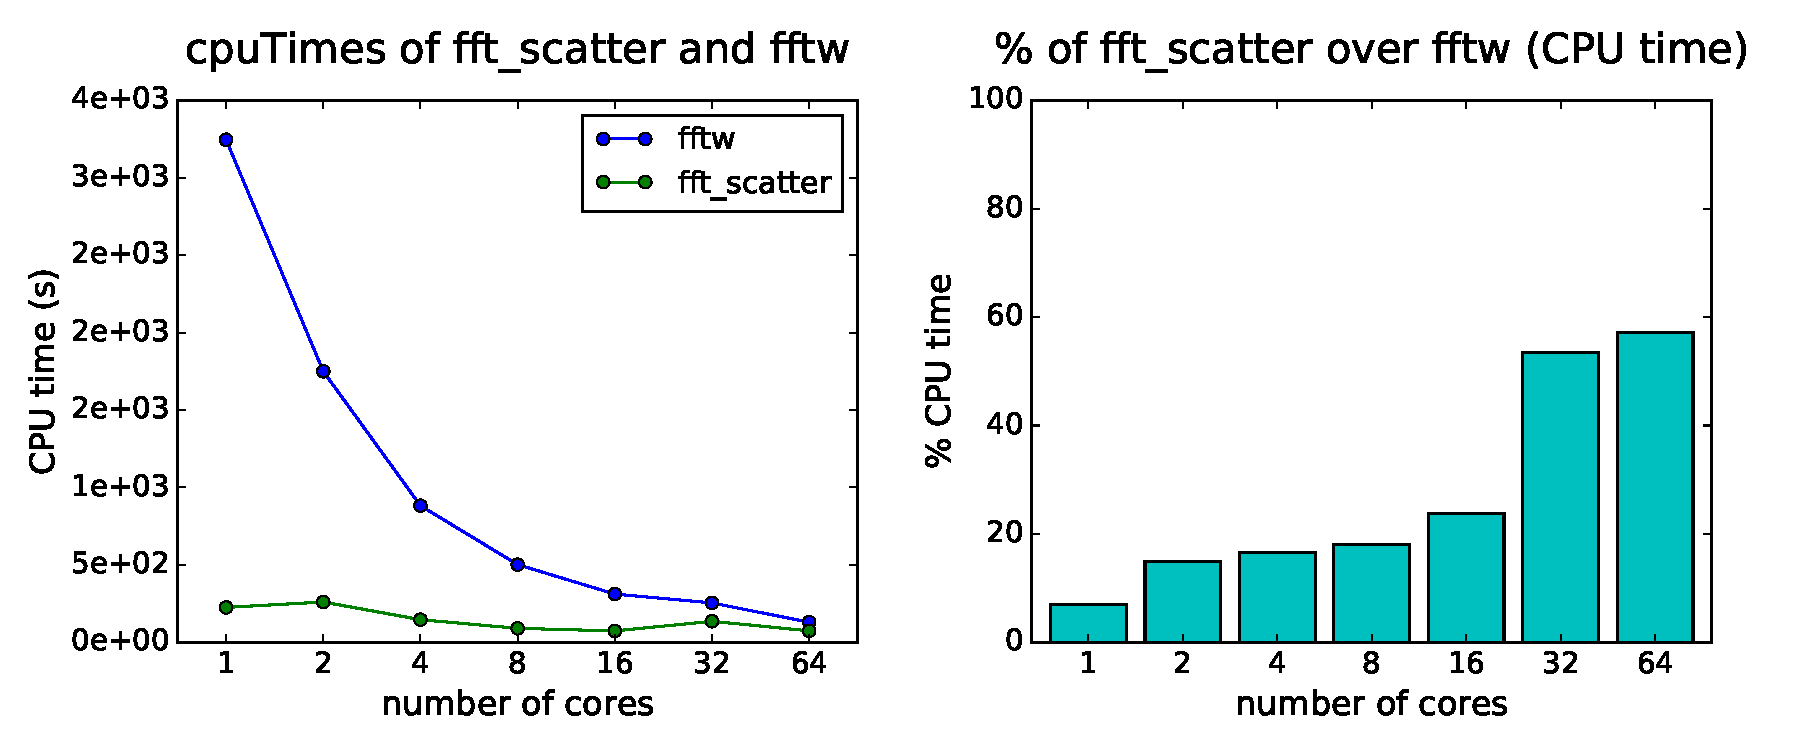
\includegraphics[width=1.2\linewidth]{fftw_vs_fft_scatter.pdf}}
	\caption{ On the left: CPU time of \texttt{fftw} and \texttt{fft\_scatter} in function of total number of core used.
	\\On the right: ratio between \texttt{fftw} and \texttt{fft\_scatter} CPU time expressed in percentage, highlighting the rising weight of communication over computation.
	}
	\label{fig:fftwvsfftscatter}
\end{figure}

We now have a clear view on where the communication happens and what kind of MPI subroutines are used.

We can also get an estimate on the weight of communication over calculation by comparing the CPU time spent in \texttt{fftw} (calculation) and \texttt{fft\_scatter} (communication) subroutines.

In the left graph of figure \ref{fig:fftwvsfftscatter} we plotted the CPU time of the two subroutines in function of the number of cores. 
\texttt{Fft\_scatter}'s CPU time is subject to little variation, but if we compare its value with \texttt{fftw}'s one we can see that communication gradually earns an increasing weight. 
In fact, as plotted in the graph on the right, we can see that CPU time ratio of \texttt{fft\_scatter} over \texttt{fftw} rises over sixteen cores, when more than two Galileo nodes, and more than four NUMA nodes ( composing two different blades), have to communicate.
A more in-depth analysis about this trend is exposed in section \ref{sec:resArchDependent}.


\newpage
\begin{center}
\begin{framed}
What is the dynamic of the SCF iteration?
\end{framed}
\end{center}

Although the question can seem undoubtedly vague, it is of capital importance in order to understand the critical aspects that rise  while profiling the behavior of a self consistent calculation.

As we have explained in section \ref{sec:SCF-DFT} and section \ref{sec:SCFConvergence} an SCF calculation is an iterative process that terminates only when self-consistency is achieved.
The number of iterations needed to reach self-consistency is not fixed nor predictable beforehand.
Hence the time necessary to obtain a physically reliable result can vary in function of a wide series of factors: size of the physical system, quality of the initial density guess, precision requested, algorithm used, number of cores employed, ... .


\begin{figure}[hhh!]
	\centerline{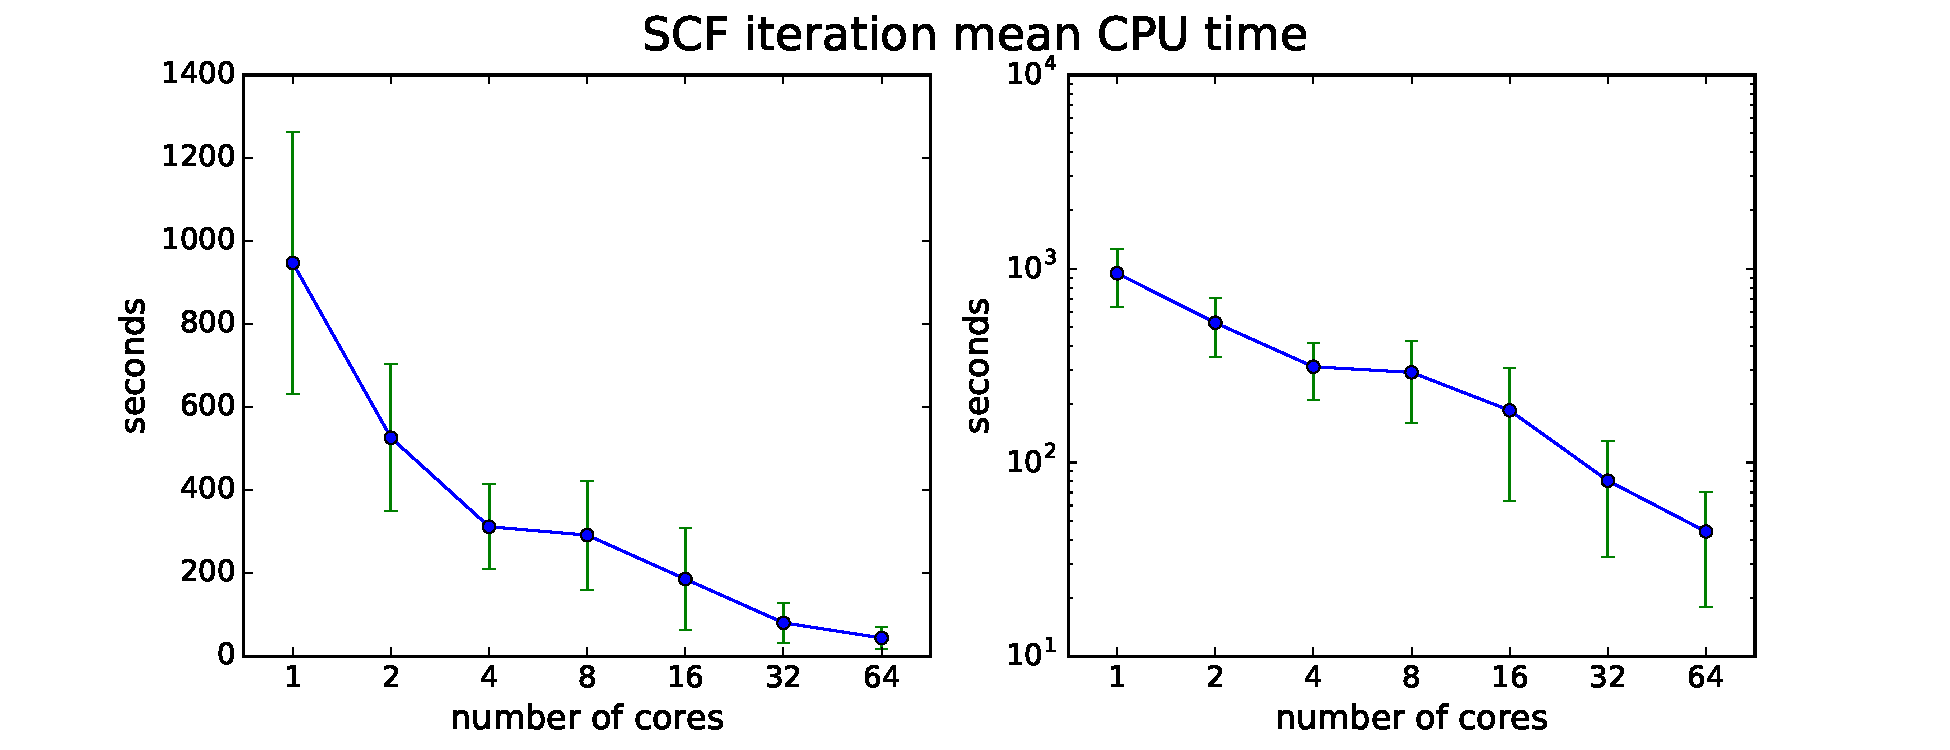
\includegraphics[width=1.2\linewidth]{iterstats.pdf}}
	\caption{ Mean iteration CPU time in seconds in function of the number of cores employed, the error bar represent the standard deviation (see table \ref{tab:iterations}.
	The plot on the right is in logarithmic scale to highlight the weight of the standard deviation.
	}
	\label{fig:iterstats}
\end{figure}

Even the time necessary to perform a single iteration step can vary considerably.
In figure \ref{fig:iterstats} we have plotted the value of mean iteration CPU time in function of the number of cores used, the error bar is the standard deviation.

We can see that the iteration time is far from being constant and varies sensibly. 
In the plot on the right we have the same data plotted in logarithmic scale to highlight the fact that the relative variation of iteration's time grows with the number of cores.
In fact, by looking at the data reported in table \ref{tab:iterations} we can see that the relative error is always above the 50\% when more than eight cores are used.


\begin{table}[hhh!]
\begin{center}
\begin{tabular}{r|cccc}
\toprule
cores &        mean iteration time(s) &         st-dev(s) &   relative error(\%) &   number of iterations \\
\midrule
1  &  676 &  201 &  29 &  43 \\
2  &  363 &  118 &  32 &  42 \\
4  &  207 &   68 &  33 &  70 \\
8  &  204 &  102 &  50 &  86 \\
16 &  154 &  109 &  71 &  55 \\
32 &   80 &   44 &  55 &  36 \\
64 &   58 &   35 &  60 &  50 \\
\bottomrule
\end{tabular}
\end{center}
\caption{Iterations statistics for self consistent calculation on variable number of cores.}
\label{tab:iterations}
\end{table}

Another important factor exposed in table \ref{tab:iterations} is that the number of iterations varies quite drastically depending on the number of cores used. 
The cause of this behavior is that the quantity $\Delta E$ used to check self-consistency (see section \ref{sec:SCFConvergence}) is used as a parameter to control the convergence of the Davidson diagonalization.
This introduces a certain amount of numerical instability that makes the number of iterations required variable.

It is somewhat reassuring that the number of iteration does not varies significantly on the two architectures we used, as exposed in table \ref{tab:architectureIterations}.

\begin{table}[hhh!]
\begin{center}
\begin{tabular}{r|ccccccc}
\toprule
cores 	 &  1  &  2  &  4  &  8  &  16  &  32  &  64 \\
\midrule
Galileo	 & 43  & 42  & 70  & 86  &  55  &  36  &  50 \\ 
UV2000	 & 43  & 42  & 72  & 83  &  55  &  36  &  50 \\ 
\bottomrule
\end{tabular}
\end{center}
\caption{Number of iteration requested to reach self consistency using different cores on two different computational architectures.}
\label{tab:architectureIterations}
\end{table}



It now appears clear why in section \ref{sec:Goals} we introduced two points of view.
In order to profile and compare the performances of PWscf and its subroutines in function of the number of cores we need to fix the number of SCF iterations performed. Otherwise the computations between two runs at different cores could be considered different.
We decided to pick 20 as a fixed number of iterations, this seems a good compromise between having a good statistic and a 
reasonable run time\footnote{Read below for a more precise justification of this choice.}.

We also want to find if it is possible to tune the architecture in order to lower the number of iteration requested to reach self consistency, i.e. to find the physical result as soon as possible. Which is a topic of great interest for the quantum chemistry and solid state physics community.
Hence the need for a more ``pragmatical" point of view.

This is why from now on we will report the results with both fixed and variable iterations.

An alternative approach, which is mainly used in industry benchmarks\cite{HPC}, is to fix the WALL time dedicated to computation and count the number of iterations performed.
This approach has two main downsides: 
first we will lose the data provided by the internal metrics, which are accountable and do not implies any form of overhead; 
second, for the data to be reliable, a reasonable number of iterations at a single core will be requested. 
In our case, for a twenty step iteration, the execution time is six hours, which would imply to reserve the computational resource for that amount of time for every test performed.
Since the time we had available was not indefinite and the resources, especially the UV2000, had to be shared without the help of a batch scheduler, we decided to fix the number of iterations and use the CPU time as a metric.

This gave us the possibility to perform many more tests and investigate more aspects of \QE scalability.

Using the mean iteration time can also be an alternative, but, as exposed in figure \ref{fig:iterstats}, it would introduce a generous amount of relative error.
Nevertheless the mean iteration time can be used as a general indicator of the dynamic of the SCF calculation.

\newpage
\begin{figure}[hhh!]
	\centerline{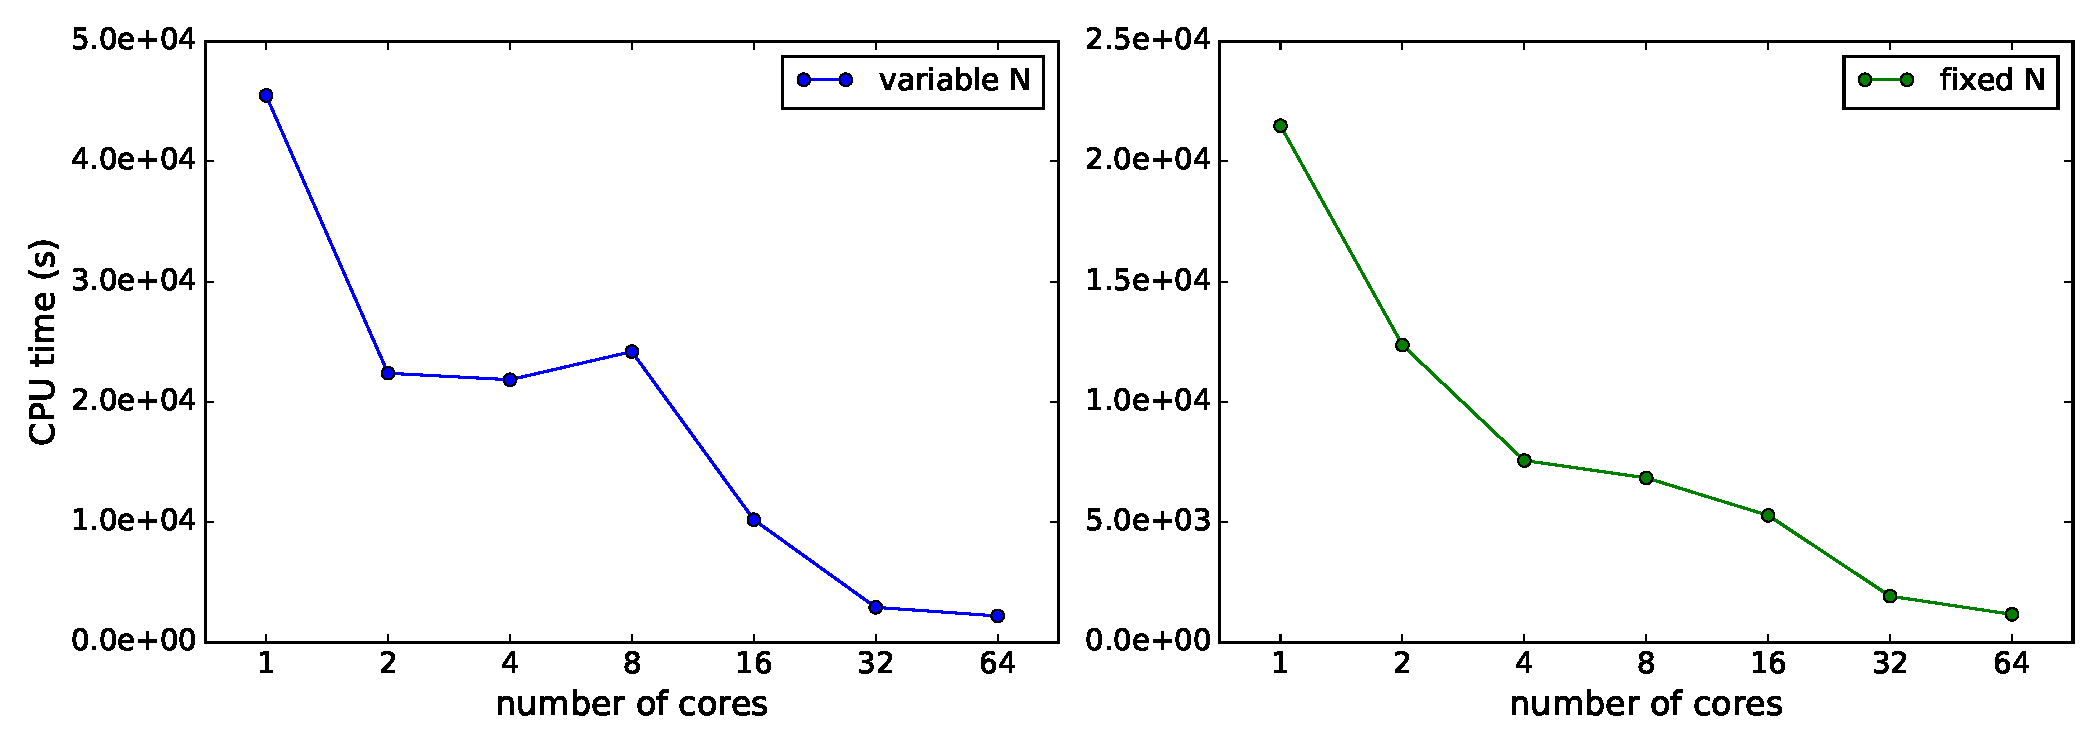
\includegraphics[width=1.2\linewidth]{fixed_vs_variable.pdf}}
	\caption{ CPU time (seconds) for variable number of iterations on the left and fixed number (20) of iterations on the right.
	}
	\label{fig:fixedvsvariable}
\end{figure}

In figure \ref{fig:fixedvsvariable} we plotted the CPU time of PWscf with variable number of iterations\footnote{i.e. until self-consistency is reached.} and fixed (twenty) number of iterations.

We can see how the CPU time is, obviously, different, since the number of iterations is not the same.
Also the shape of the two curves is clearly different.
It is clear that the excessive number of iterations reported in table \ref{tab:iterations} causes a rise on the execution time of the left plot.
Nevertheless in the right plot it appears that the decreasing trend slows at eight and sixteen cores. This means that even excluding the bias of variable iterations, the computation does not performs efficiently in that range of the core scale.
The analysis of this behavior and one possible way to optimize the code efficiency is reported in section \ref{sec:resArchIndependent}.



\newpage
\subsection{Architecture Independent Tuning}\label{sec:resArchIndependent}

To investigate the behavior exposed in figure \ref{fig:fixedvsvariable} we can plot the CPU time and speedup for the relevant functions listed in section \ref{sec:resCriticalComponents}.

\begin{figure}[hhh!]
\centerline{ 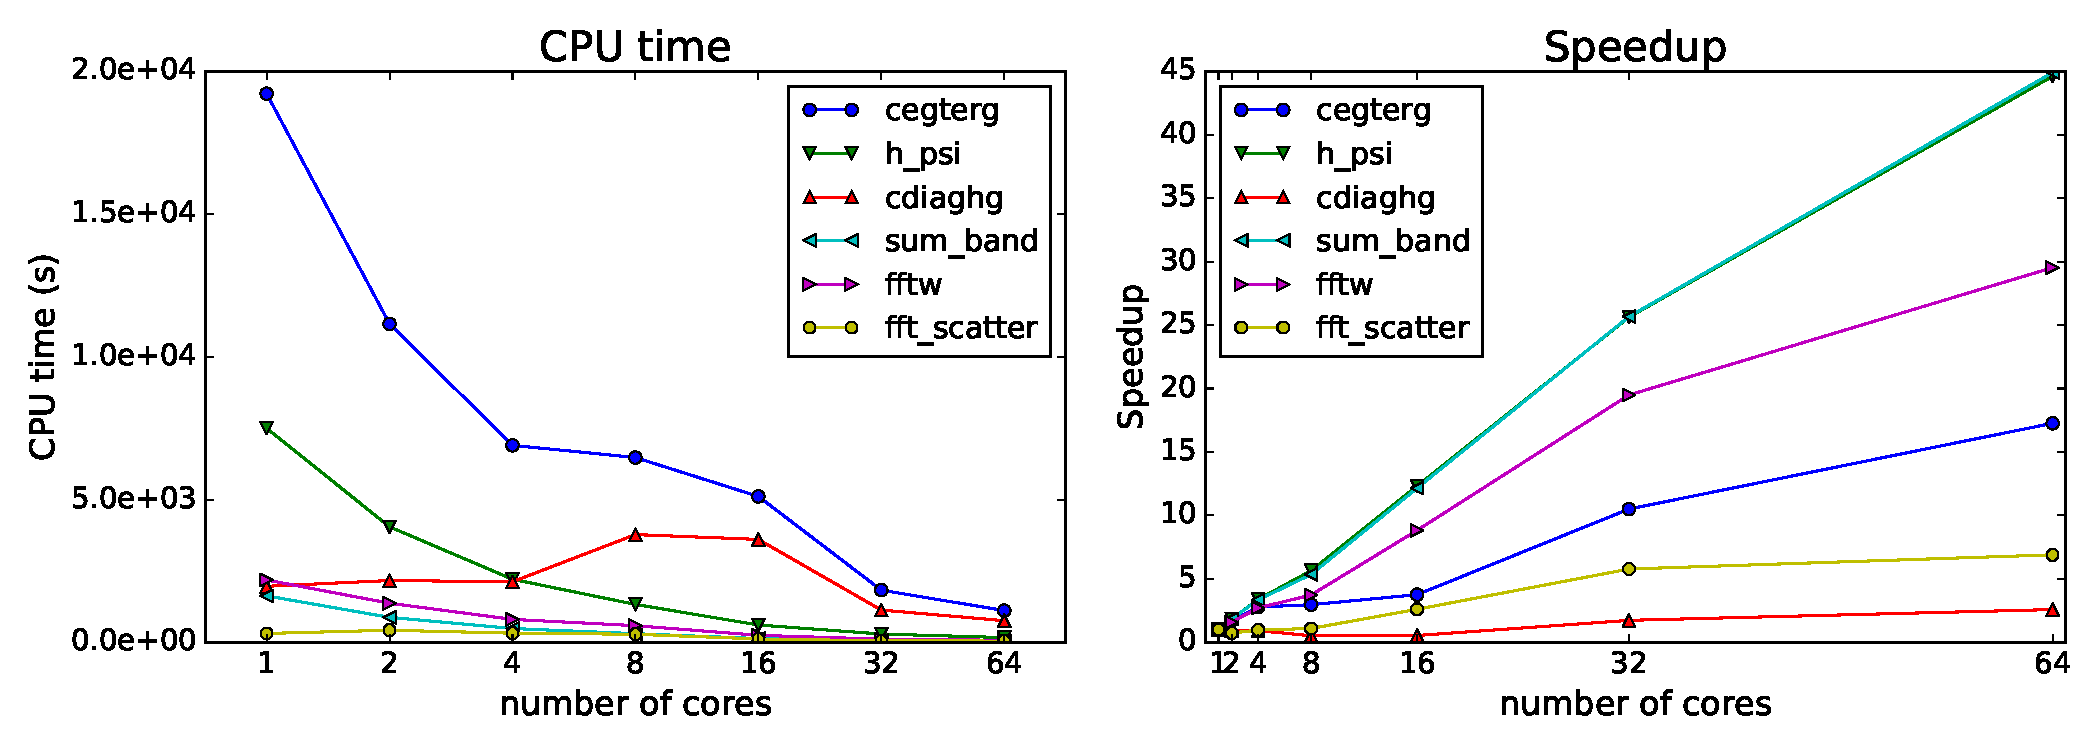
\includegraphics[width=1.2\linewidth]{relevant_subroutines.pdf}	}
	\caption{CPU time (left) and speedup (right) for relevant subroutines listed in section \ref{sec:resCriticalComponents}. Data from runs at fixed number of SCF iterations.}
	\label{fig:relevantSubroutines}
\end{figure}

As said in section \ref{sec:resCriticalComponents}, we can use \texttt{cegterg}  as a reference for PWscf execution time.

\texttt{H\_psi}, which is one of the two main actors in \texttt{cegterg}, scales remarkably well. Its speedup is close to linear and the efficiency\footnote{Speedup over number of cores.} is always above the 70\%. 
So does \texttt{sum\_band}, as expected for what we said in section \ref{sec:QE}.
It is clear that the scalability problem must lie withing \texttt{cdiaghg}.

In fact we can see that its CPU time remains the same at one and two cores, increases lightly at four cores and almost doubles at eight and sixteen cores. 
Its behavior is far from being efficient and its speedup its practically flat compared to the others functions.

First of all we need to understand what is happening and how \QE performs the diagonalization in function of the number of cores when threads are not used.

The first thing to notice is that at one and two cores the diagonalization is performed serially, only by the first MPI rank. This is why the CPU time of \texttt{cdiaghg} is the same at one and two cores.

Starting at four cores a different approach is used: a parallel and full memory distributed ScaLAPACK diagonalization is performed \cite{QE2}.

%core/core diagonalizzazione
%8/4
%16/4 -> perche' non ne usa 9! 3x3! -> basta dirgli -ndiag 9
%32/16
%64/25
%

It is clear that on a relatively low number of cores the distributed diagonalization is counterproductive.

The easiest way to affect diagonalization performance, especially in the low cores range, is to introduce the use of threads.


Threads are a second level of parallelization that operates within a single MPI rank.

The main difference between thread parallelization and MPI is that MPI is a message passing protocol, it must perform communication to distribute data between different processes, while threads works in a shared memory environment and do not need to communicate explicitly between each others. 
Threads usually operates concurrently on separated chunks of memory, performing the same operation on different data at the same time.


\QE implements threads using the OpenMP (OMP) standard interface\cite{OMP}.
Note that not all the subroutines in \QE uses this kind of parallelization, hence some sections of the code remain still serial.
This is the main reason why the use of threads can lead to different behavior and, in general, their tuning must be performed carefully.

Speaking of threads distribution, what the user can do is to assign a number of threads to each MPI rank.
This is done setting the \texttt{OMP\_NUM\_THREADS} environmental variable to the desired number of threads.

In general it is suggested that the total number of threads must not exceed the number of physical cores on the resource (see appendix \ref{app:Threads}).

The total number of threads can be obtained easily by multiplying the number of threads per MPI rank times the number of MPI ranks.
For example if we have a 64 core resource and we want to use 16 MPI ranks, the number of threads per MPI rank should not exceed 4.

This flexibility generates a wide range of possible combinations, especially when the number of core increases.

In appendix \ref{app:Threads} we reported the results of our tests for all the possible combinations, both for fixed and variable number of SCF iterations.

From the data exposed in appendix \ref{app:Threads} we have composed two optimal set of runs for fixed and variable \footnote{The difference is only at 32 cores.} number of iterations.
The general rule was to keep the best result per total number of cores employed.\footnote{ The total number of cores is the number of MPI ranks times the number of threads per rank.}

The results, compared with the runs without threads, are exposed in figure \ref{fig:threadsOverall}.

\newpage 

\begin{center}
\begin{framed}
What is the overall impact of thread parallelization?
\end{framed}
\end{center}


\begin{figure}[hhh!]
\centerline{ 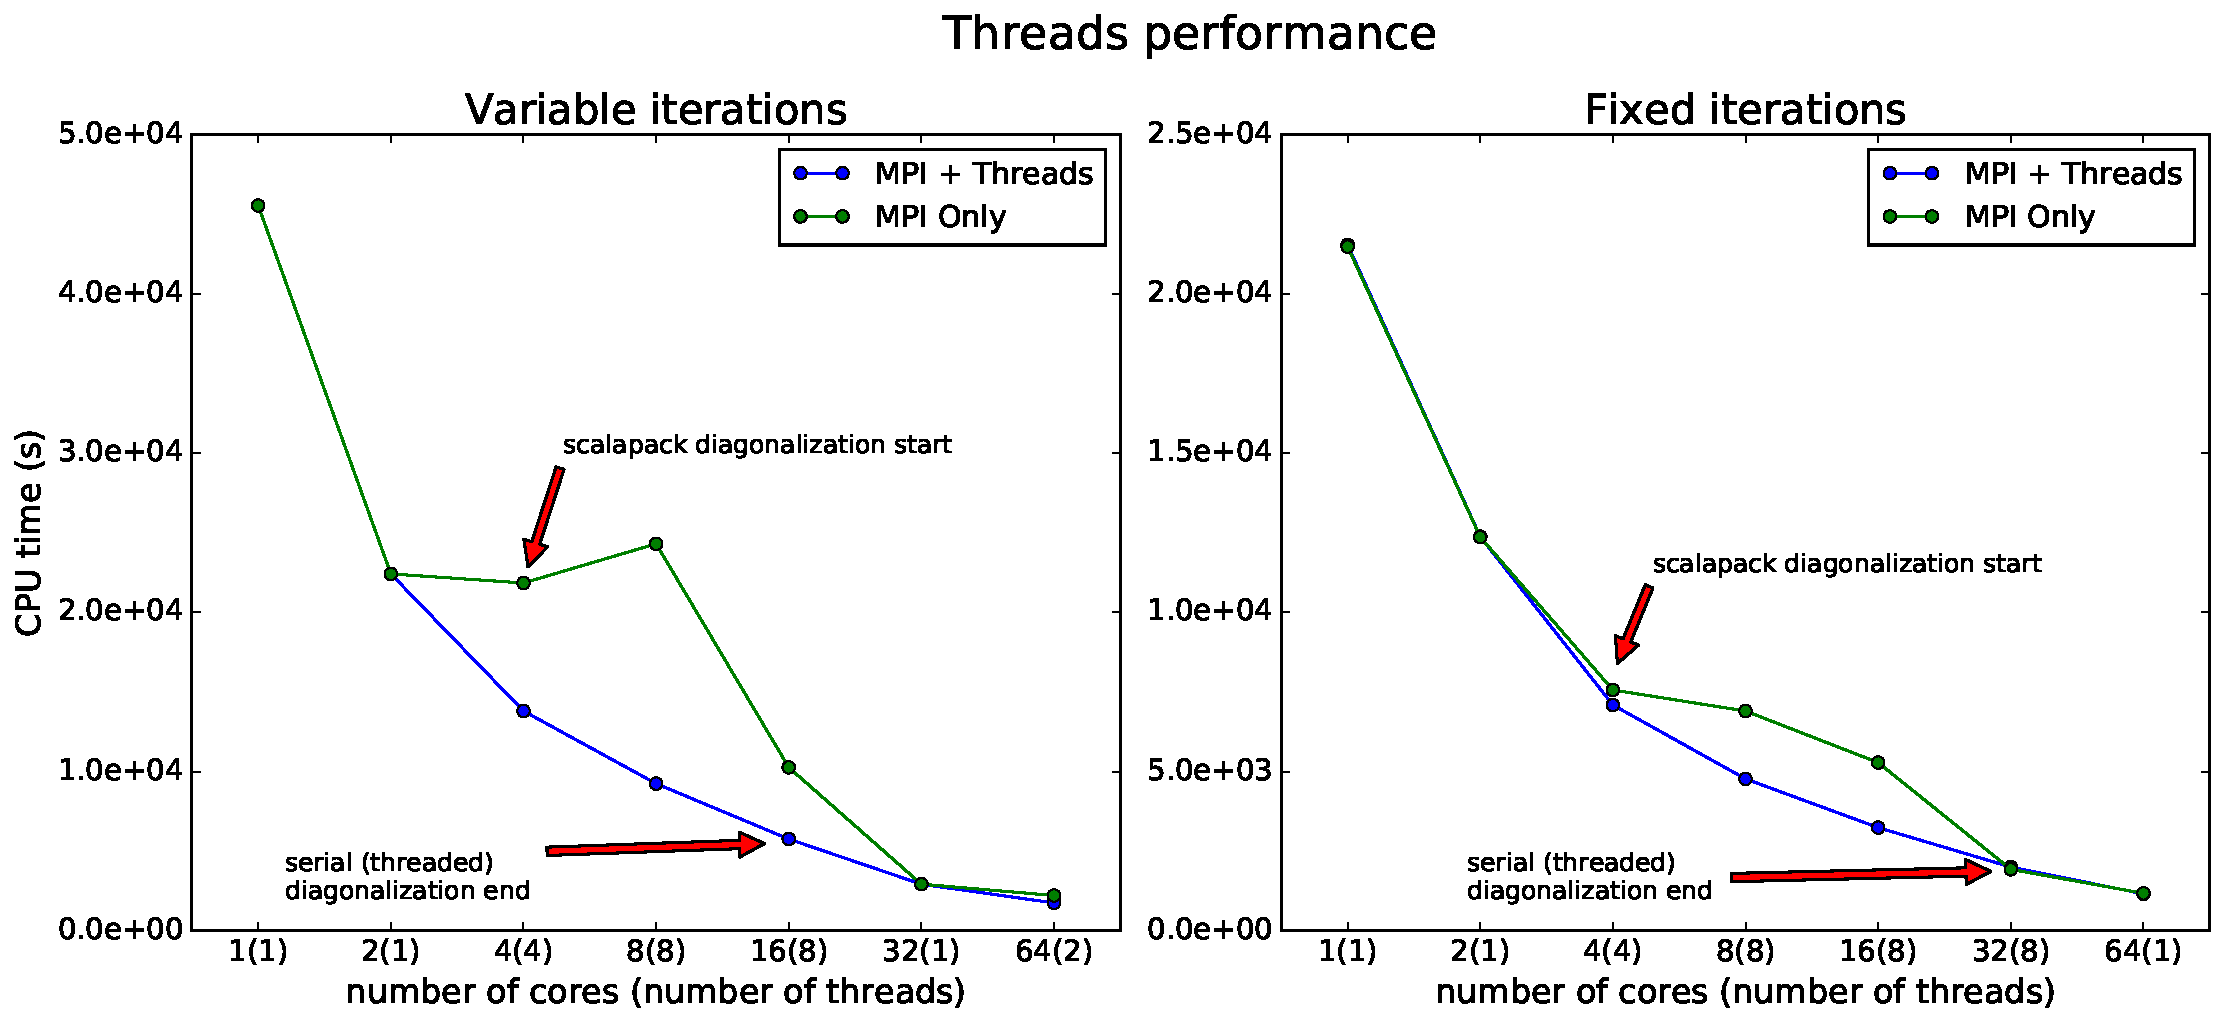
\includegraphics[width=1.2\linewidth]{threads_overall.pdf}	}
	\caption{PWscf's CPU time at variable number of iterations (left) and fixed number of iterations (right). Both threaded (``MPI + Threads") and not threaded (``MPI Only") runs are plotted. On the x axis are reported the total number of cores and the number of threads per MPI rank for the threaded run.}
	\label{fig:threadsOverall}

\end{figure}

On the x axis we have reported the total number of cores and, in parenthesis, the number of threads per MPI rank (see above).
To obtain the number of MPI ranks used just divide the number of cores for the number in parenthesis.

Starting from the plot on the left we can see that, at variable number of iterations, threads have a clear and positive impact on the overall performance.
The spike at eight cores disappears completely and the descending trend of the CPU time is much more regular, hence efficient.

The result can be directly imputed to a reduction of the number of iterations needed to reach self-consistency.
In fact, we can see in table \ref{tab:threadsIterations} that the number of iterations is reduced up to 50\% ( at eight cores).

\begin{table}[hhh!]
\begin{center}
\begin{tabular}{r|ccccccc}
\toprule
cores 	 &  1  &  2  &  4  &  8  &  16  &  32  &  64 \\
\midrule
MPI Only & 43  & 42  & 72  & 83  &  55  &  36  &  50 \\ 
MPI + Threads &  47  &  42  &  43  &  43  &  42  &  36  &  36 \\ 
\bottomrule
\end{tabular}
\end{center}
\caption{Number of iterations needed to reach self-consistency for threaded and not threaded PWscf runs.}
\label{tab:threadsIterations}
\end{table}



This improved numerical stability can be attributed to the different algorithm used to diagonalize the Hamiltonian. 
In fact, on such a low number of cores, the use of threads forces PWscf to permorm a serial diagonalization instead of the distributed one, granting a faster convergence.

We have annotated in figure \ref{fig:threadsOverall} when distributed diagonalization starts on MPI only runs and when serial diagonalization ends on threaded runs.

But the benefits of threads are not restricted to numerical stability.
In fact, by looking at to plot at fixed number of iterations, on the right of figure \ref{fig:threadsOverall}, we see that (especially at eight cores) the advantage is still substantial.

Note that the gain obtained from eight to sixteen cores cannot be ascribed to the effect of threads because the number of threads used is the same and the diagonalization algorithm is serial.

To get a deeper understanding on what routines benefit from threads we need to investigate our metrics at fixed number of iterations.


\newpage

\begin{center}
\begin{framed}
What is the impact of thread parallelization on each component?
\end{framed}
\end{center}


\begin{figure}[hhh!]
\centerline{ 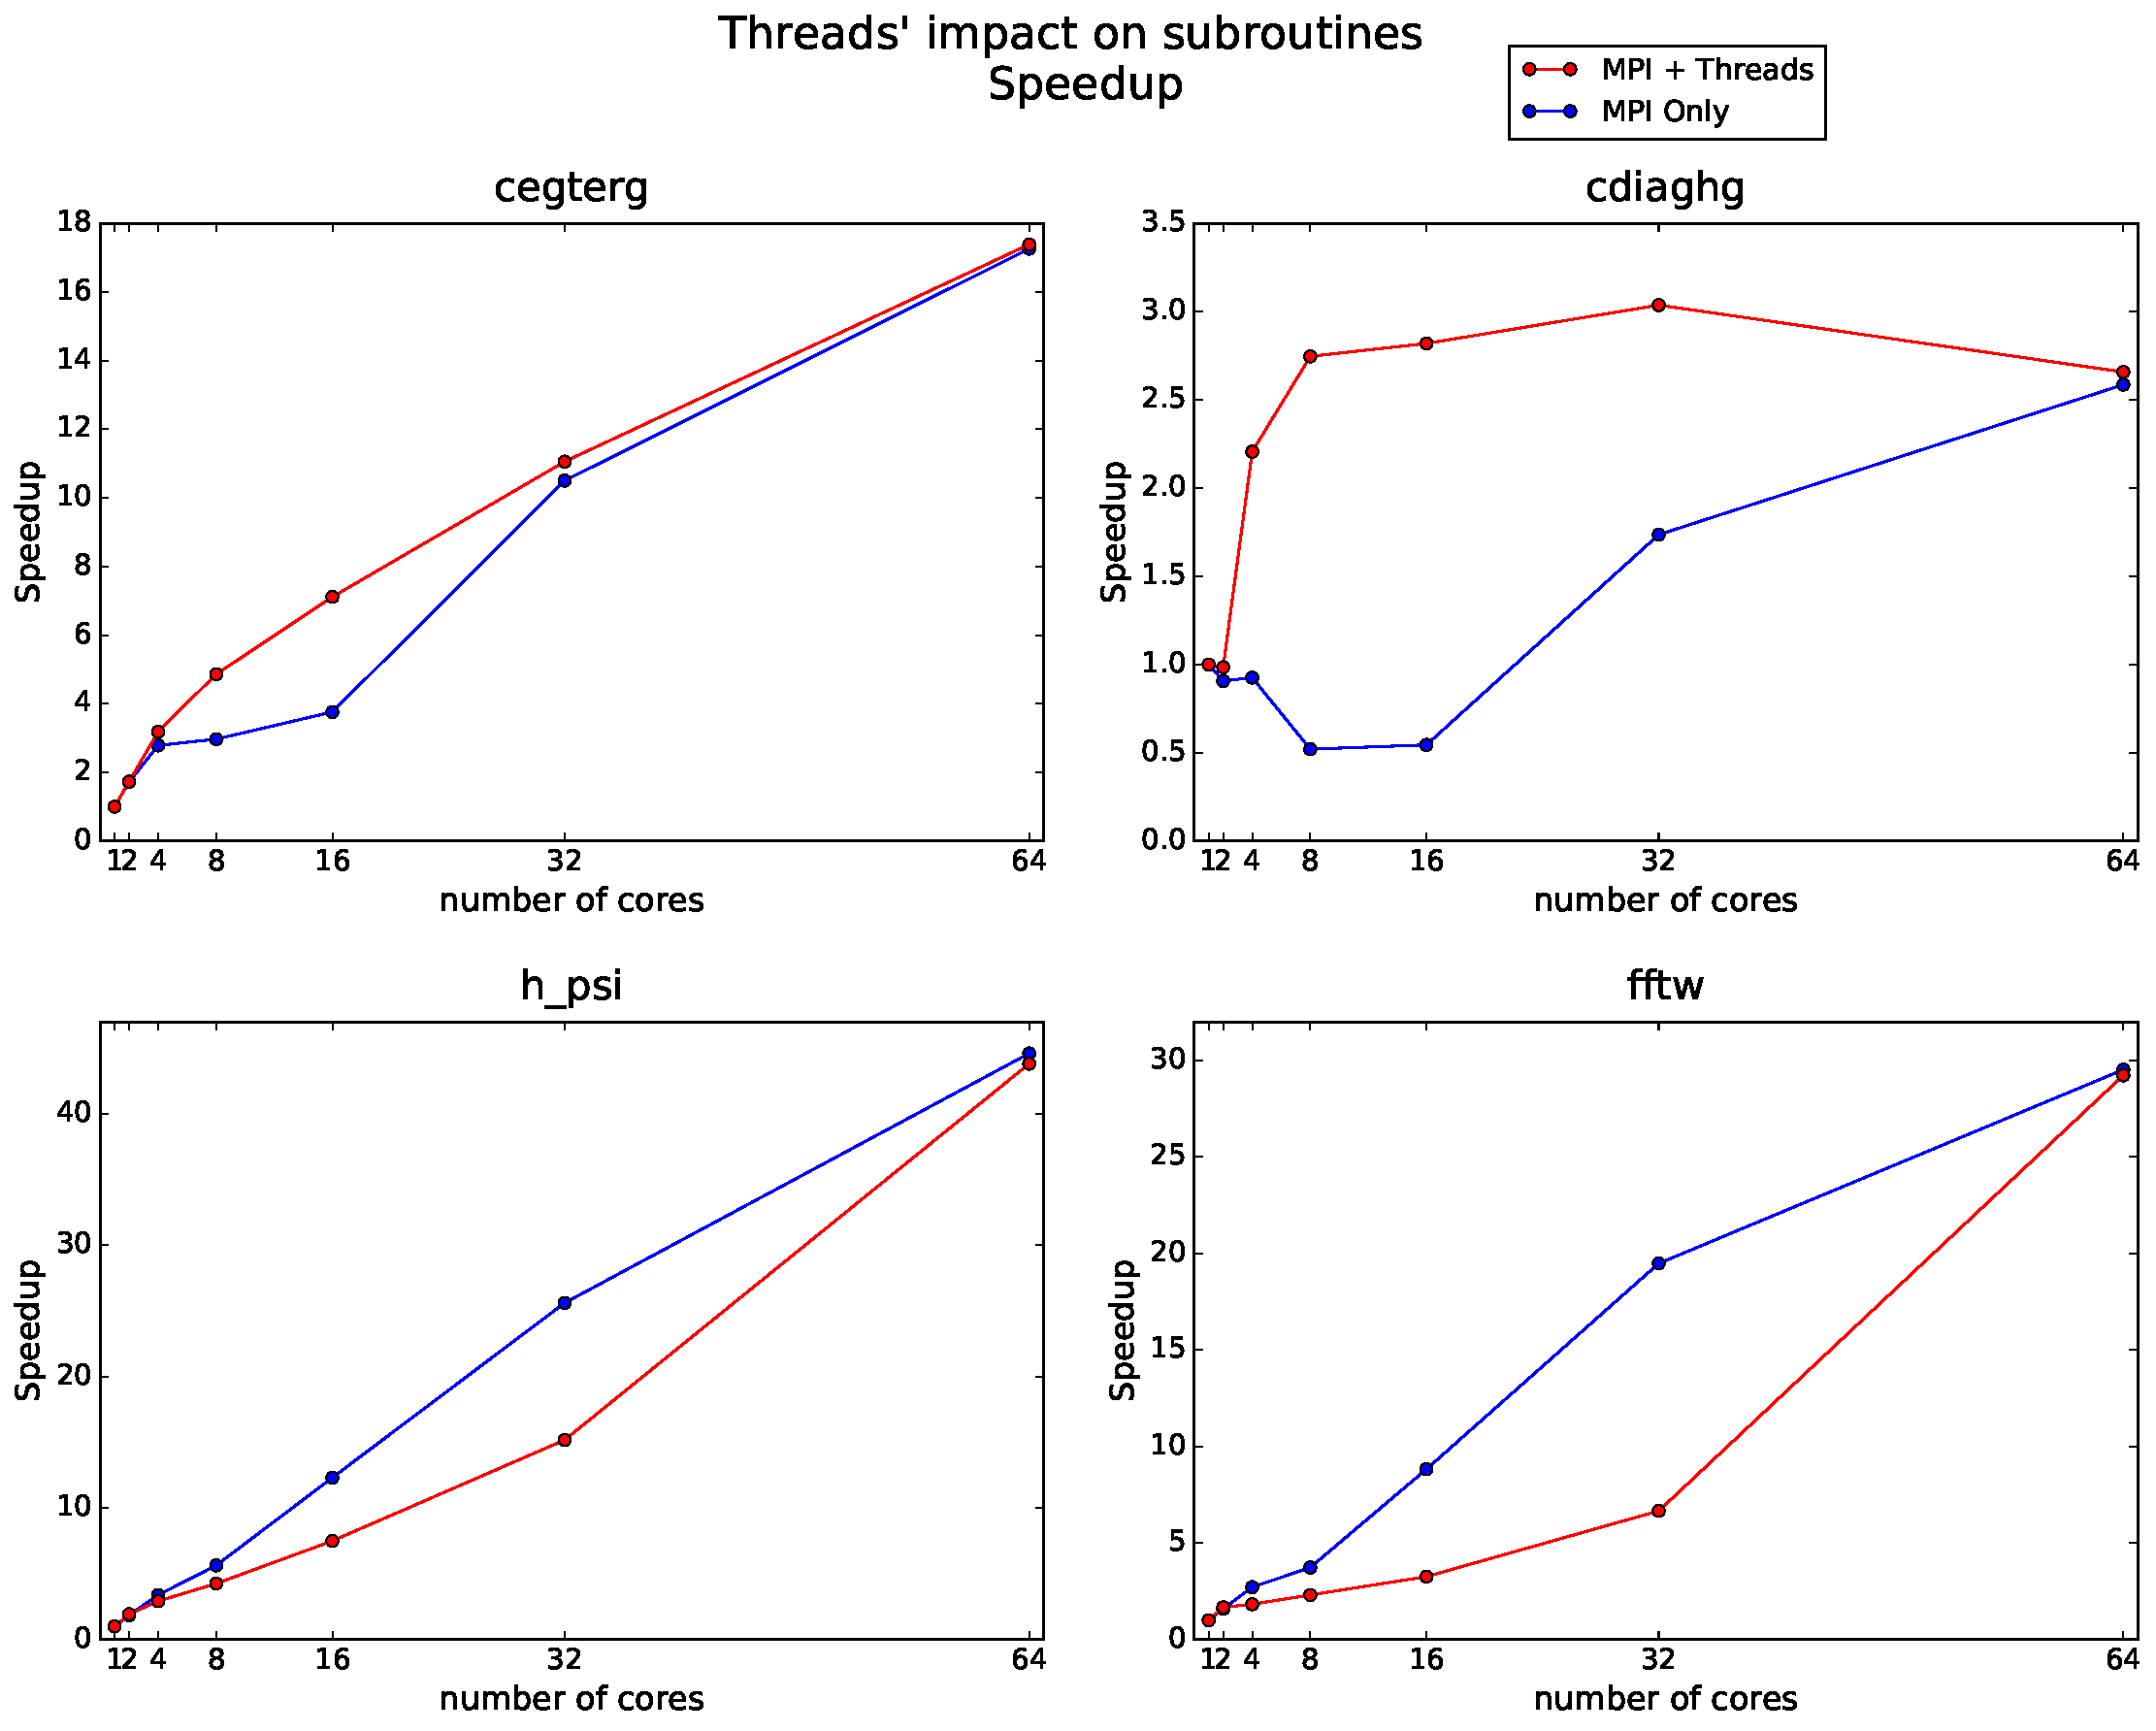
\includegraphics[width=\linewidth]{threads_subroutines.pdf}	}
	\caption{Speedup of relevant subroutines at fixed number of iterations for threaded and not threaded PWscf's runs from one to sixteen cores.}
	\label{fig:threadsSubroutines}

\end{figure}


The plot of \texttt{cdiaghg}'s speedup in figure \ref{fig:threadsSubroutines} tells us that threads benefit mainly diagonalization\footnote{The fact that speedup does not change from eight to sixteen cores confirm what we have said above.}.
While, on the contrary, the impacts on \texttt{h\_psi} and \texttt{fftw} performance is counterproductive.

This means that a loss in performance of \texttt{h\_psi} in exchange of a more efficient diagonalization can sensibly improve the overall performance of the SCF cycle when a low number of core is used (as reported in \texttt{cegterg} plot).

A very important note: remember that PWscf was always compiled with full support of threaded mkl libraries \footnote{Linear algebra package for Intel compilers.}, otherwise threads would have no effects on diagonalization's performance because PWscf don't explicitly use threads for serial diagonalization.


\begin{center}
\begin{framed}
In which scenario is convenient to use thread parallelization?
\end{framed}
\end{center}

From the results exposed in in figure \ref{fig:threadsOverall} and \ref{fig:threadsSubroutines} the straightforward conclusion is that threads are appealing when a low\footnote{Comparable to the number of cores on the chipset} number of cores is used.

This opens two possible scenarios of interest.

\paragraph{High throughput computing (HTC):} 
When the time needed to perform a particular simulation loses importance in front of the necessity to complete a large number of simulations, threads can be very appealing, especially when studying systems with similar dimensions and atomic species.
To maximize the number of simulations completed one could perform a set of tests on a trial system and determine the right number of threads to obtain a reasonable efficiency.

From the data reported in figure \ref{fig:threadsOverall} and appendix \ref{app:Threads} we can extract a simple ``rule of thumb" to find the best number of threads and cores:
it seems convenient to fill the chipset with the maximum number of threads, that is to use a single MPI rank for chipset and as many threads as the cores on the chipset.
For example: in our case we would have chosen one MPI rank spawning eight threads\footnote{Both the architectures have an eight core chipset.}, obtaining an efficiency of 60\%\footnote{Efficiency is defined as speedup over number of cores.}.

Then schedule a massive submit of jobs to the preferred batch system. 
This approach can also be very appealing since large HTC pools with batch schedulers like Condor\cite{Condor} are increasing in popularity and can be adopted with little cost by universities and institutions.

\paragraph{Owned resources instead of shared clusters:}
Nowadays multi-core personal computers are very popular among researchers. 
It is also common for research groups to have a small cluster with multi-core nodes.
Given the price of high performance communication hardware, it is often preferred to have cluster nodes with a generous number of cores rather than an high performance interconnect.
We know also that on big shared multicomputers (like Galileo), job queues can get very long when hundreds of users are using it. Also the amount of CPU time is often parceled, hence it must be spent carefully.
For this reasons it could be more convenient to tune threads usage and perform the calculation in house rather than wait for the job to be scheduled on an overloaded cluster.


~

It is difficult to find both in literature (\cite{QE},\cite{QE2}) and in industrial benchmarks\cite{HPC}, that threads can have a meaningful impact on \QE performances.

This is because all these benchmarks focus on large scale computing, typically starting at least from 64 cores, up to thousands of cores.
Although these data are of great interest, not all the scientific community operates on such a large scale.

One must also consider that a great optimization effort was dedicated to increase the performance of the evaluation of $\mf{H}^{KS}$\footnote{The remarkable scaling of \texttt{h\_psi} described at the beginning of this section proves the results of this optimization effort.}, which translates in a more efficient FFT calculation (see section \ref{sec:QE}). 
Threads in this case have proven to be of little, if none, benefit. 
See \cite{FFTPAPER} for an detailed analysis.
See section \ref{sec:resArchDependent} for a clear view of \texttt{h\_psi} and \texttt{fftw} speedup on different architectures.

\begin{figure}[hhh!]
\centerline{ 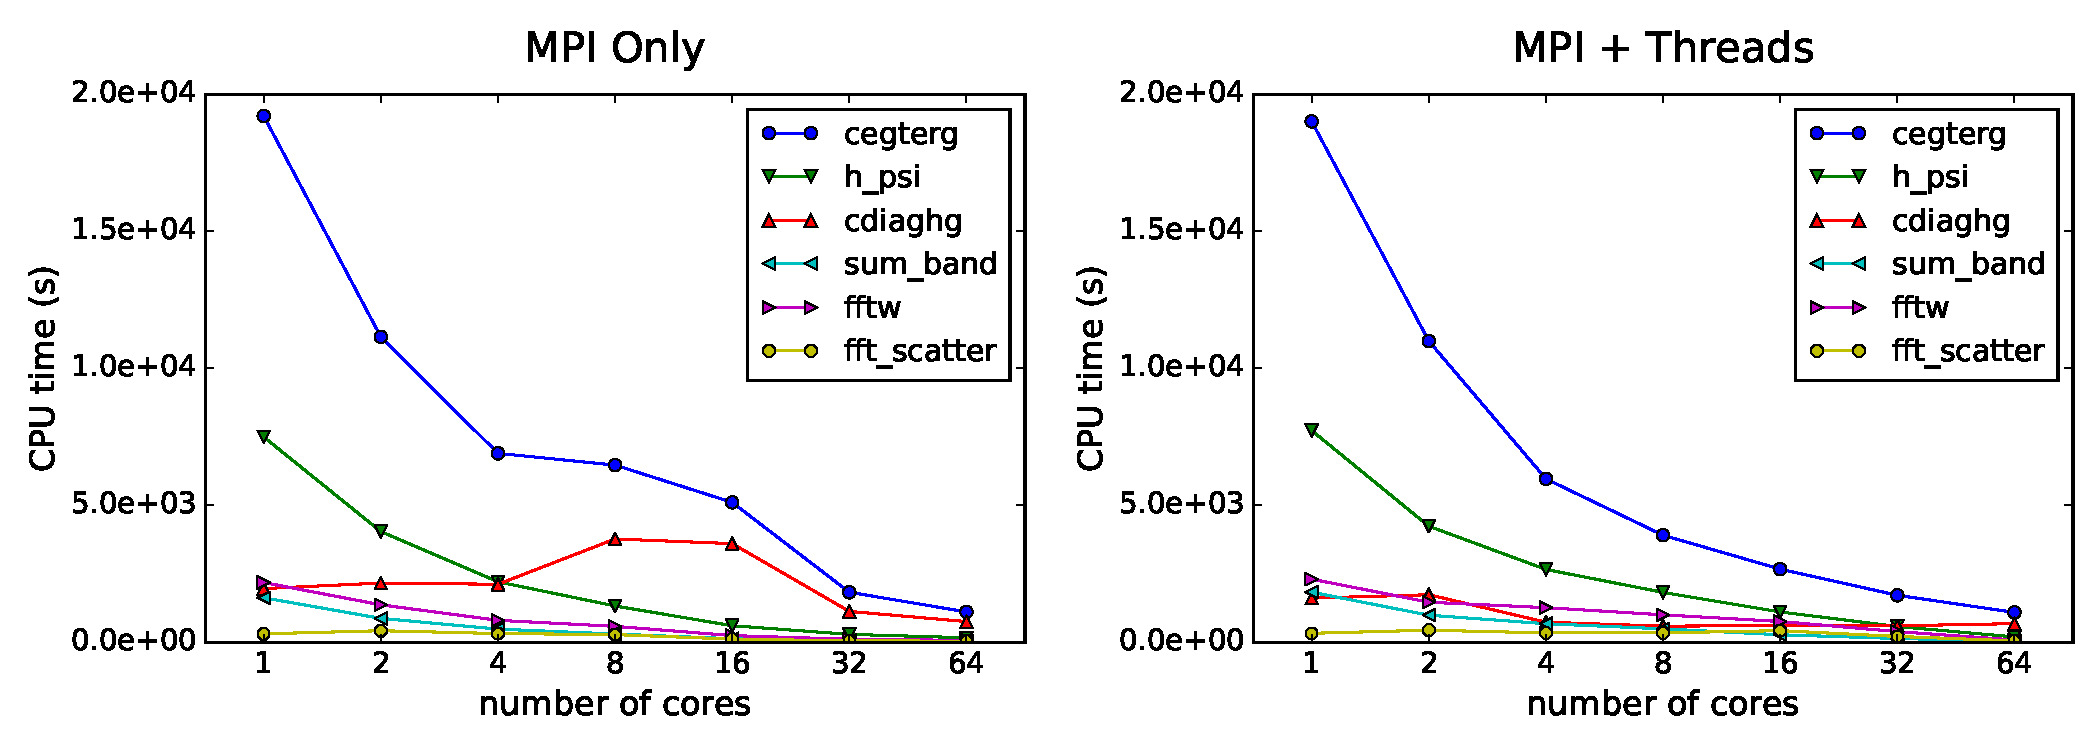
\includegraphics[width=1.2\linewidth]{threads_comparison.pdf}	}
	\caption{CPU time of relevant subroutines at fixed number of iterations with (right) and without (left) thread parallelization.}
	\label{fig:threadsComparison}
\end{figure}

As a final point we re-propose in figure \ref{fig:threadsComparison} the same metrics of figure \ref{fig:relevantSubroutines} with and without threads parallelization.

\newpage
\subsection{Architecture Dependent Tuning}\label{sec:resArchDependent}
\begin{center}
\begin{framed}
	What is the overall performance on each architecture?
\end{framed}
\end{center}

\begin{figure}[hhh!]
\centerline{ 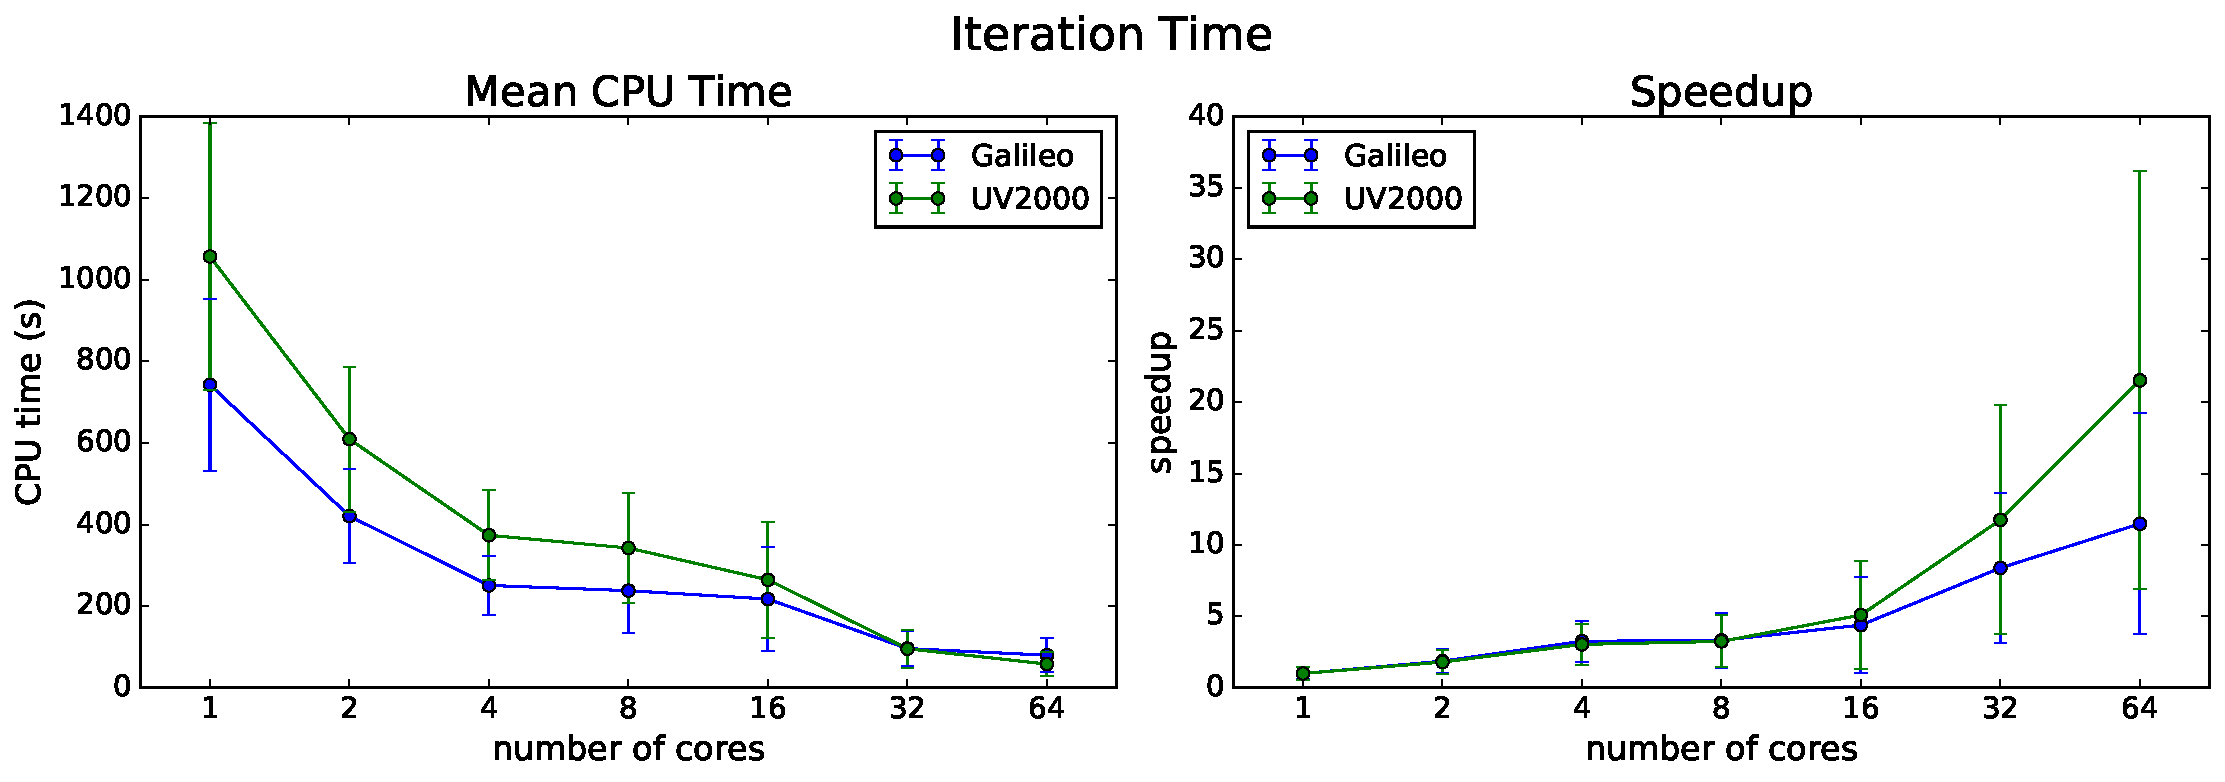
\includegraphics[width=1.2\linewidth]{arch_compare_iterations.pdf}	}
	\caption{Mean iteration time and its speedup on Galielo and UV2000 architectures.}
	\label{fig:archCompareIterations}
\end{figure}

To begin we analyze the mean iteration time of PWscf on both architectures in order to have a general idea (see section \ref{sec:resCriticalComponents} to understand the validity of mean iteration time).

At first sight, looking at the left plot of figure \ref{fig:archCompareIterations}, one will conclude that Galileo is better suited to perform \QE simulations because its CPU time is lower in a wider range of the curve.
This is true, but note that the x axis is not on a linear scale, but on a logarithmic scale (in base 2)\footnote{Given the presence of error bars, this kind of display was favored since it does not overcrowd the left part of the plot.}.

Note also that the time gap between the two architectures lowers as the number of core rises. 
At 32 cores we have the same performance and at 64 cores the UV2000 outperforms Galileo.

By comparing the speedup (right plot of figure \ref{fig:archCompareIterations}) we can get a picture on what architecture is scaling the best.

As we were suspecting, the speedup of UV2000 marks a sensible improvement after eight cores.
To get a more precise idea it is convenient to look at the PWscf execution CPU time.


\begin{figure}[hhh!]
\centerline{ 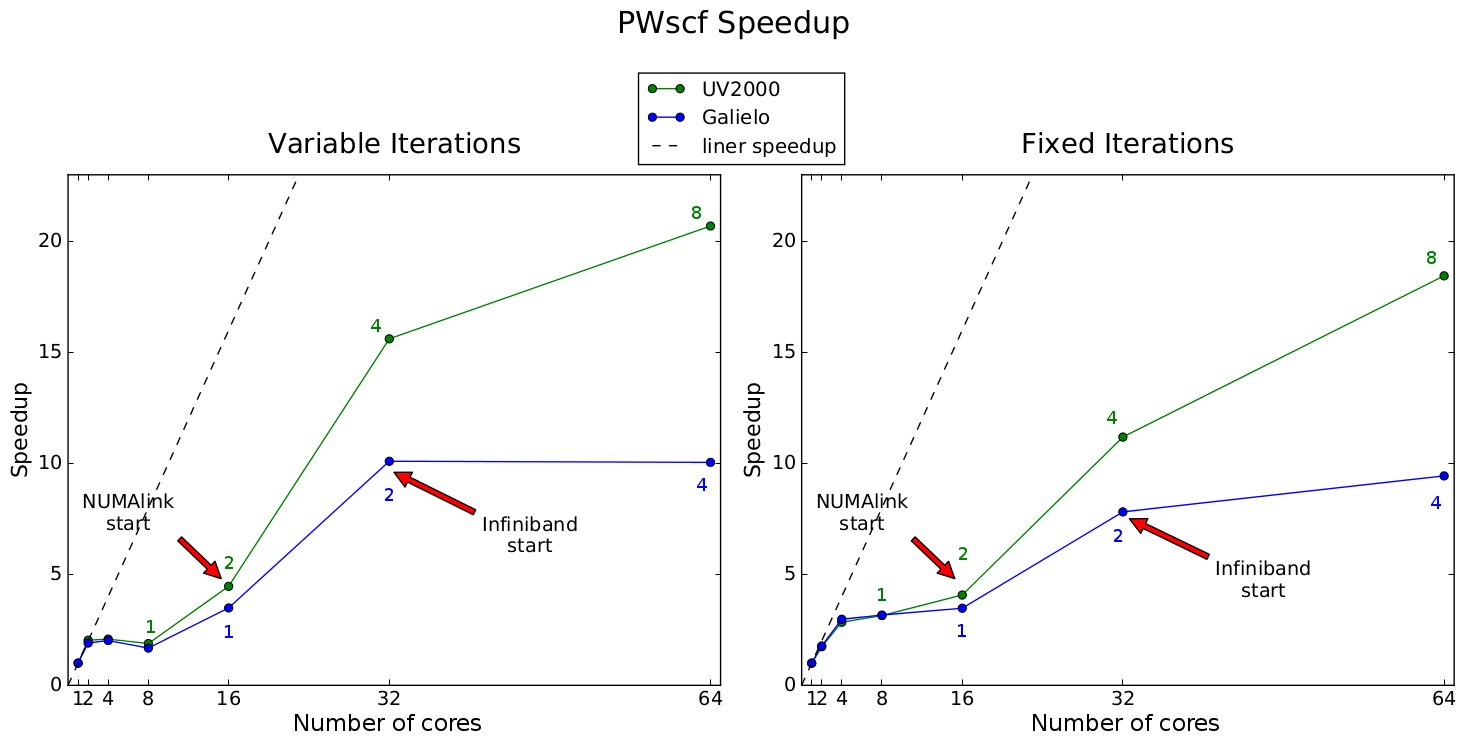
\includegraphics[width=1.2\linewidth]{arch_global_2.jpg}	}
	\caption{CPU time speedup at variable (left) and fixed (right) number of iterations on both architectures. The number of NUMA nodes is annotated in green, while the number of cluster nodes is in blue.}
	\label{fig:archGlobal}
\end{figure}

In figure \ref{fig:archGlobal} it's reported the speedup on both architectures\footnote{Which, we remind, is the correct way to compare different architectures.}



The first thing to note is that on the left plot the speedup from 32 core to 64 is flat for Galileo, while still increases for the UV2000. 
This means that the extra number of iterations reported in table \ref{tab:architectureIterations} completely voids the improvement given by the increased number of cores. 
Hence the UV2000 is clearly outperforming Galileo because the number of iterations are the same for both architectures for a given number of cores.

The plot at fixed iterations confirms this impression. 
The difference in scaling starts at sixteen cores and rises steadily with the number of cores.

Considering also the topology of the architecture we can find a first explanation on the nature of this difference.
In figure \ref{fig:archGlobal} we have marked in green the number of NUMA nodes used and in blue the number of cluster nodes employed.

It is evident that when PWscf leaves the borders of a single Galileo machine (32 cores), and Infiniband interconnect is necessary for communication, the impact on performance is negative.
On the contrary, on the UV2000, communication between nodes starts at sixteen cores, exactly when the speedup difference starts to increase.
The difference continues to increase from 32 to 64 cores, when the number of Galileo nodes communicating is four.

This happens both at fixed and variable iterations, excluding the difference in iteration numbers from the possible causes of bias.

Following the same steps of the previous section, we analyze the performance of the relevant subroutines.


\begin{center}
\begin{framed}
What are the components that performs best on each architecture?
\end{framed}
\end{center}




\begin{figure}[hhh!]
\centerline{ 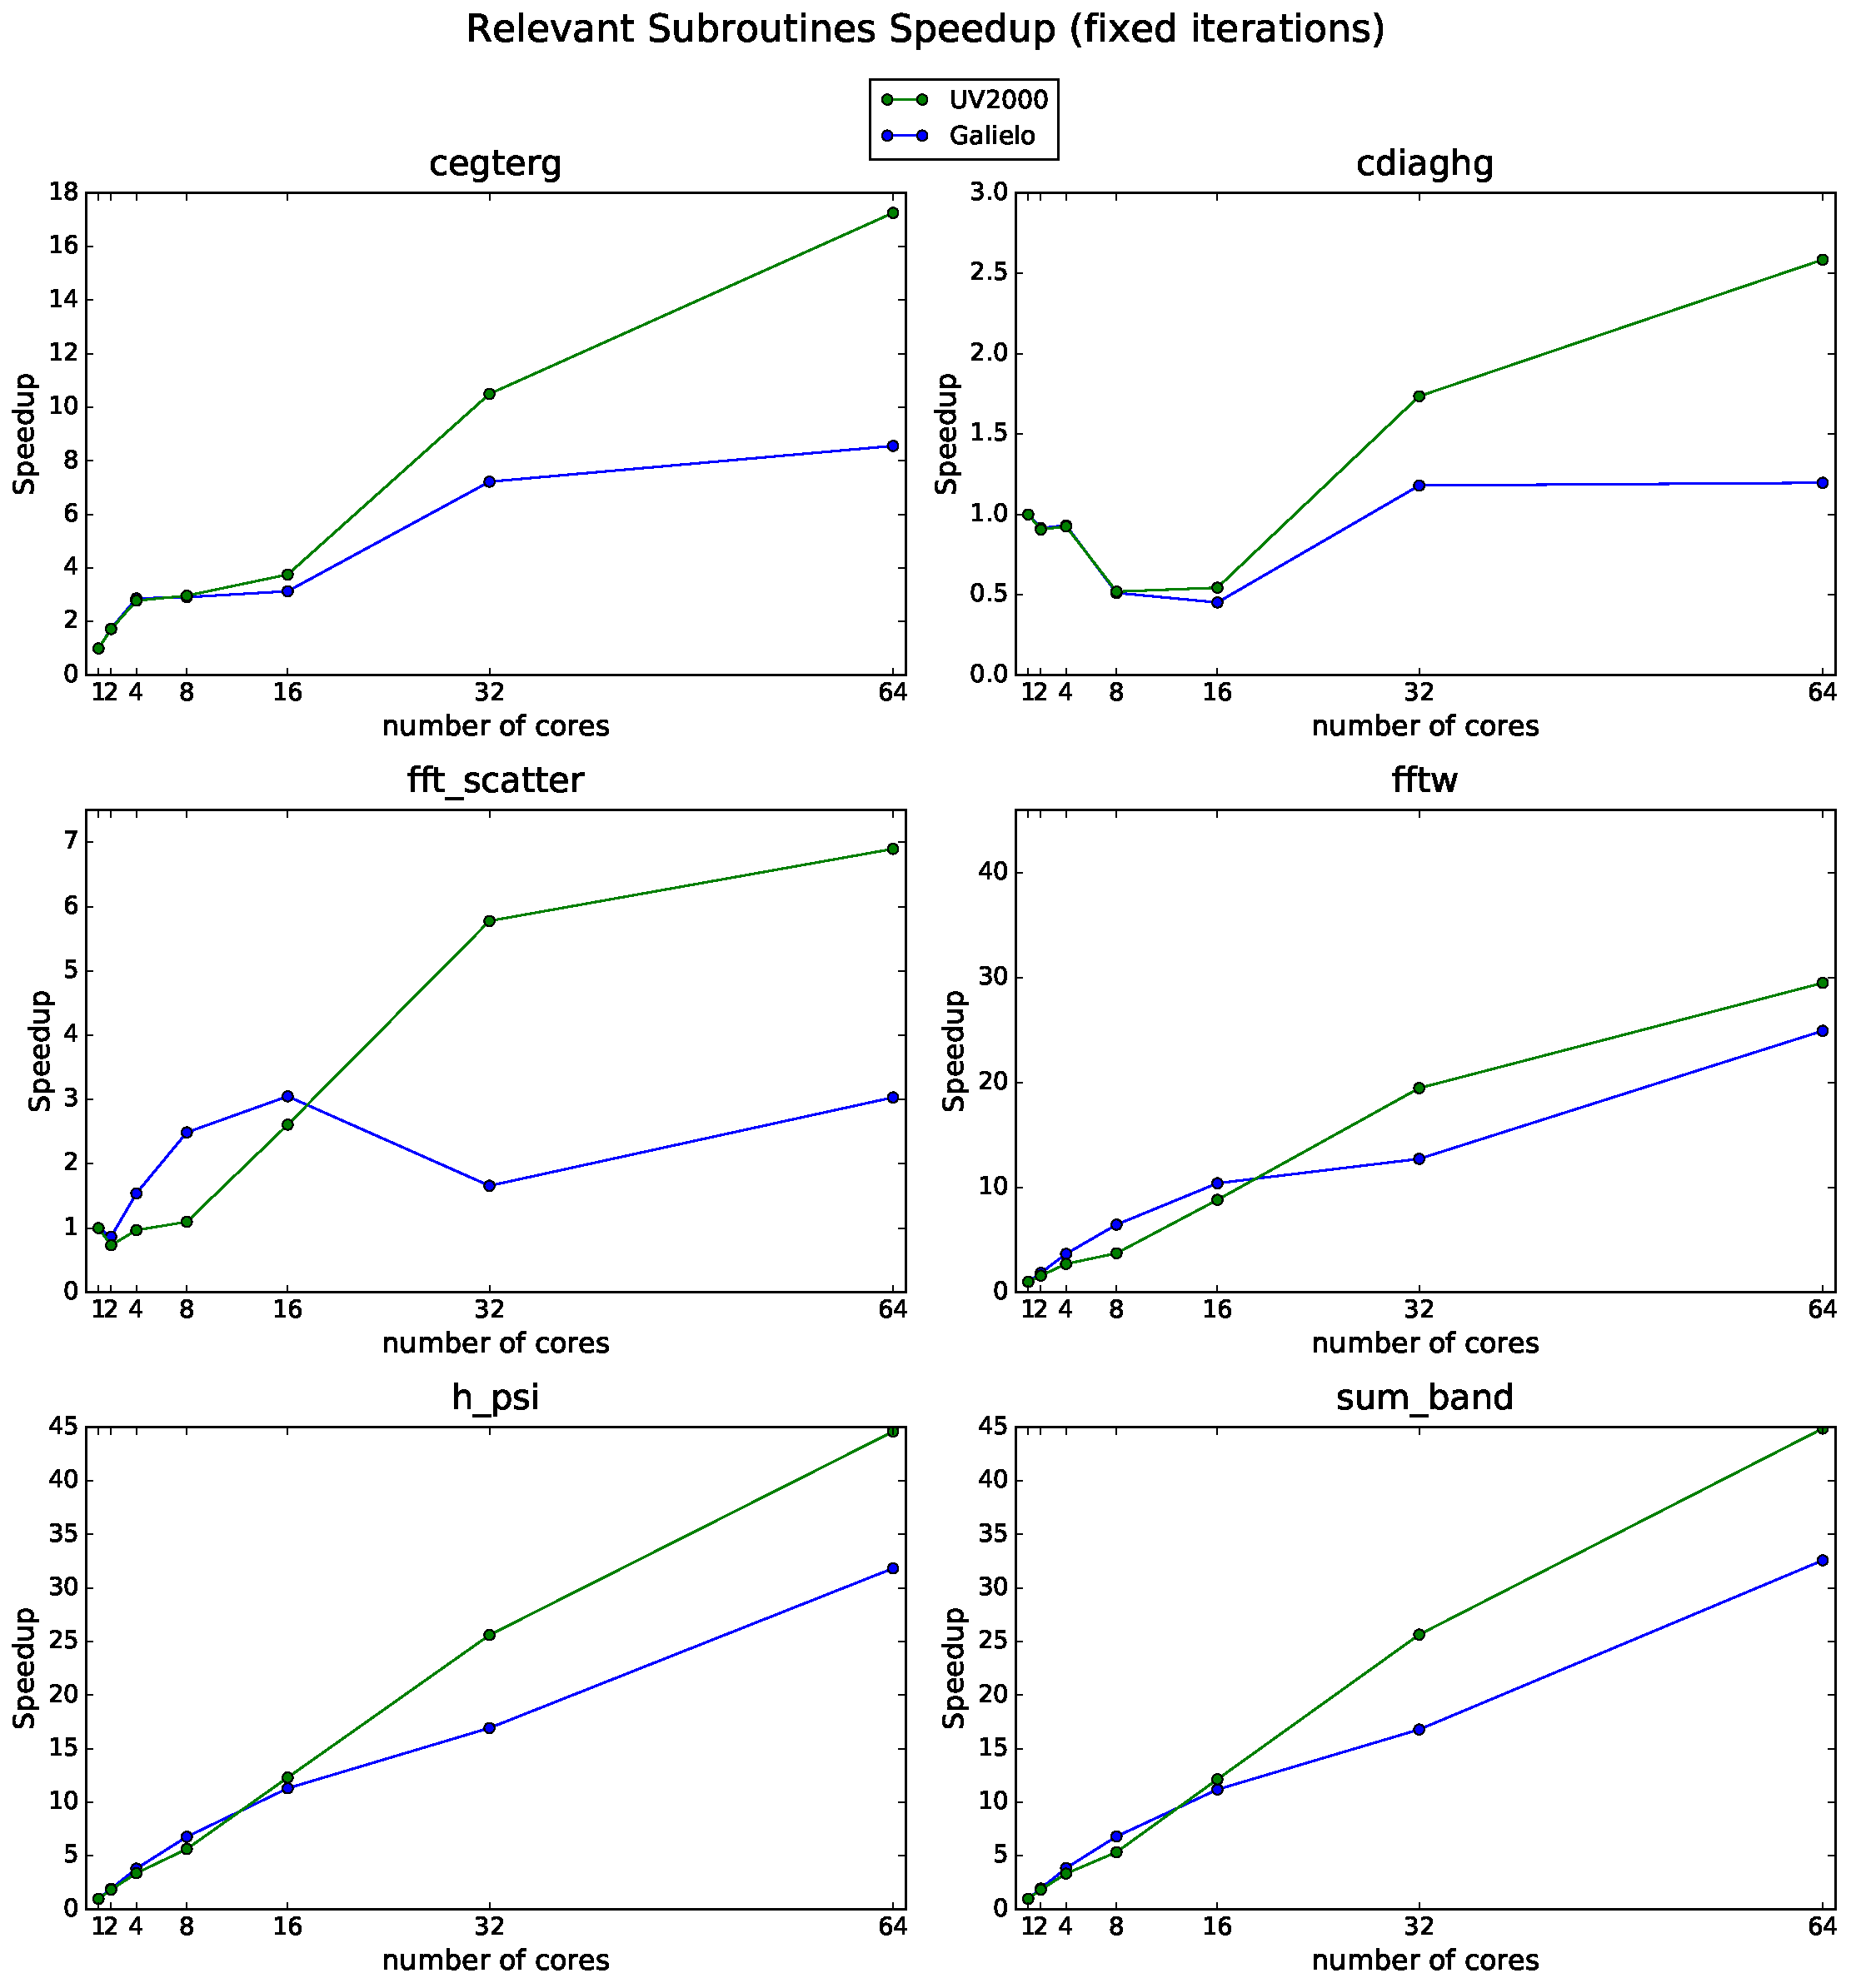
\includegraphics[width=1.2\linewidth]{arch_subroutines.pdf}	}
	\caption{tempo totale}
	\label{fig:archSubroutines}
\end{figure}


In figure \ref{fig:archSubroutines} is plotted the speedup at fixed number of iterations for all the relevant subroutines listed in section \ref{sec:resCriticalComponents}.
As expected, the two main actors, \texttt{h\_psi} and \texttt{cdiaghg} starts to improve on the UV2000 when more than one NUMA node is needed.

While \texttt{c\_diag} mantains a low speedup, at least on the UV2000 the performance rises above sixteen cores.

The speedup of \texttt{h\_psi} and \texttt{sum\_band} are very similar, as expected from what said in section \ref{sec:QE}, and incredibly linear (compared with \texttt{c\_diagh}). 
This highlights a very efficient parallelization of matrix evaluation.

This is confirmed by the speedup of \texttt{fftw}, that constitutes a considerable part of matrix evaluation(see section \ref{sec:Diagonalization}).

Finally, the plot of \texttt{fft\_scatter}\footnote{We remind that \texttt{fft\_scatter} is a subroutine that performs manily communication.} strongly suggests that communication is performed very differently on the two architectures.


It seems time to investigate at a deeper level what is the performance of interprocess communication on the two architectures.

\newpage
~
\newpage

\begin{center}
\begin{framed}
What architecture has the best implementation of interprocess communication?
\end{framed}
\end{center}



\begin{figure}[hhh!]
\centerline{ 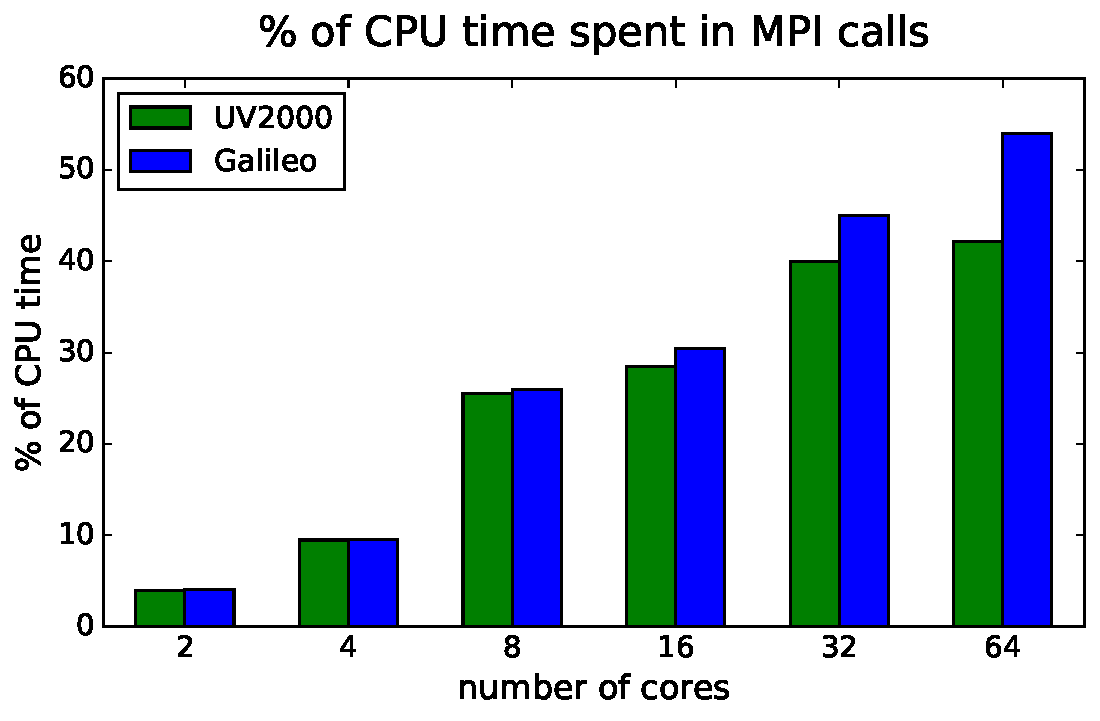
\includegraphics[width=0.7\linewidth]{arch_mpi_perc.pdf}	}
	\caption{Percentage of time spent in MPI communication. Metrics provided by \texttt{scorep} and analyzed with \texttt{scorep-score}.}
	\label{fig:archMpiPerc}
\end{figure}


Figure \ref{fig:archMpiPerc} reports the total percentage of time (calculated over PWscf CPU time), spent in MPI communication.

We can see that the number increases particularly after 16 cores, as expected, and that it is a remarkably high percentage.

On both architecture more than 40\% of the CPU time is spent in communication when the number of cores is more than sixteen, this is a considerably high number and points out that communication plays a central role in tuning the architecture performance.

We can see also that Galileo spends more time in communication compared to the UV2000, and the gap increases with the number of cores.

It is important to note that this plot cannot justify a 2x speedup difference between the two architectures, as exposed in figure \ref{fig:archGlobal}.

Keep also in mind that ScaLAPACK internal communication is not profiled\footnote{See section \ref{sec:resCriticalComponents}} and, according to \cite{QE} and \cite {QE2}, it is considered to have a very high impact communication volume.

Nevertheless figure \ref{fig:archMpiPerc} tells us that UV2000 has a better implementation of the MPI library and constitutes a valid indication that communication as an important impact on PWscf performances.

\newpage
\begin{center}
\begin{framed}
	How diagonalization distribution impacts on PWscf performance on both architectures?
\end{framed}
\end{center}

All the data we have analyzed so far points out an important information.
Matrix diagonalization constitutes a major bottleneck in this kind of simulations.

Obviously this observation is true considering also that matrix evaluation has been finely optimized by \QE developers.

We still have one way to affect how diagonalization is performed (besides threads), but this option is effective only on a sufficiently high number of cores.
To be more clear, we need to explain how matrix multiplication is perfomed by \QE when four cores or more are used.

\QE uses the Cannon's algorithm\cite{Cannon} for parallel matrices multiplication\cite{QE2}. 
This algorithm needs to distribute the matrices\footnote{Which in our case are always squared!} in a bi-dimensional grid of ``actors", in our case actors is a synonym of MPI rank.
This implies that the number of ranks dedicated to the matrix diagonalization is $n^2$ where $n$ is a natural number.
Hence, given our resources, the possible values are as follows:
\begin{equation*}
	n_{diag} = n^2 = 4 , 9 , 16 , 25 , 49 , 64 .
\end{equation*}
Obviously $n_{diag}$ cannot exceed the total number of cores destinated to PWscf.

To set the number of cores dedicated to diagonalization it is sufficient to use the \texttt{-ndiag} PWscf's argument.

In appendix \ref{app:ndiag} we reported the results for PWscf's CPU time at fixed number of iterations in function of $n_{diag}$. 
In figure \ref{fig:ndiag64} we reprint the data for a run at 64 cores.

\begin{figure}[hhh!]
\centerline{ 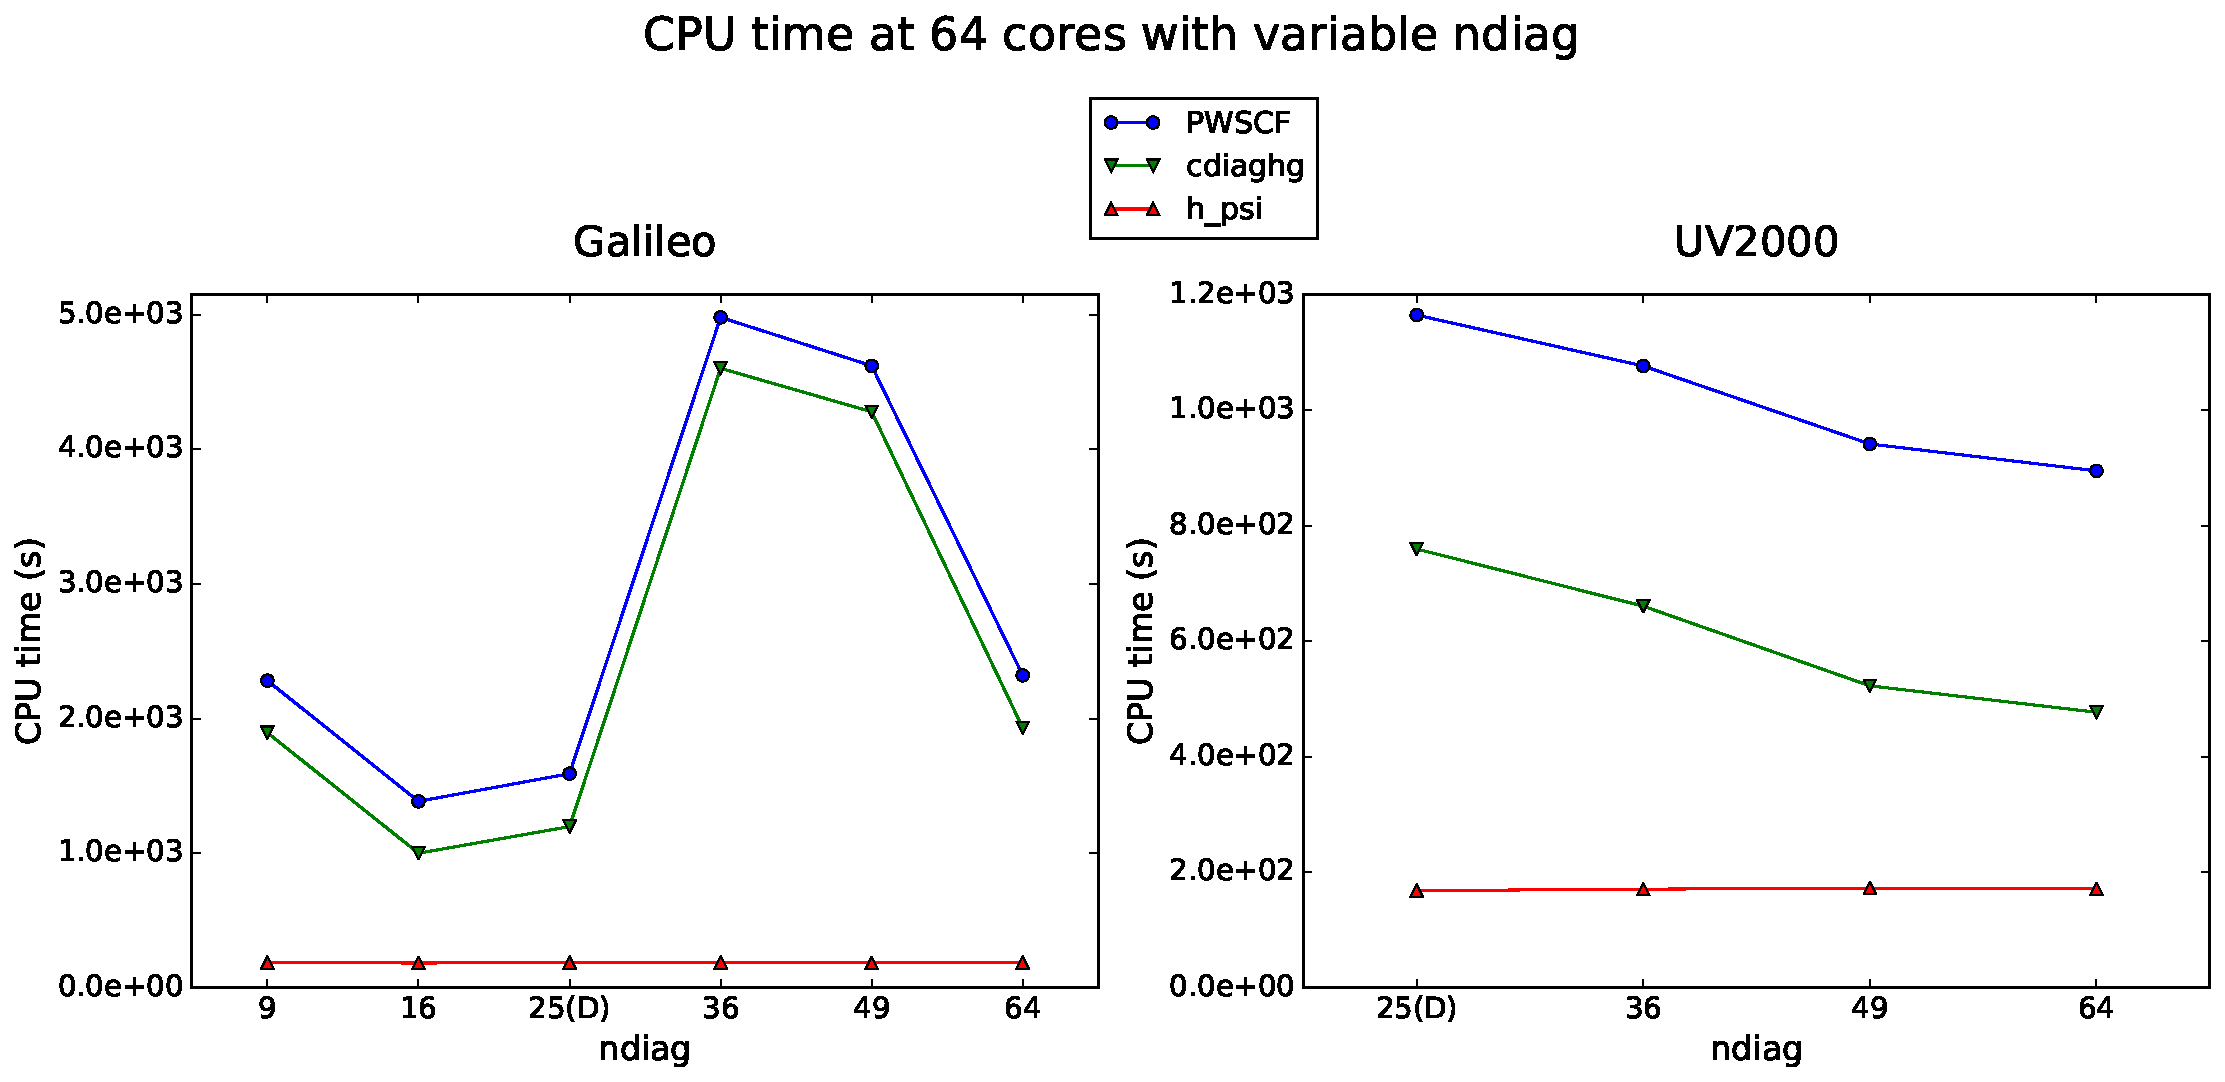
\includegraphics[width=1.2\linewidth]{ndiag_64.pdf}	}
	\caption{CPU time of a 64 core PWscf's run in function of the number of ranks dedicated to diagonalization $n_{diag}$.}
	\label{fig:ndiag64}
\end{figure}

First of all it is confirmed that \texttt{-ndiag} affects only the performance of \texttt{cdiaghg} and not \texttt{h\_psi}'s ones.
Hence the overall speedup can only be attributed to \texttt{cdiaghg} optimization.
In fact PWscf's curve and \texttt{cdiaghg}'s curve are identical.

We can see also that the behavior of the two architectures is, once again, different.

Starting from Galileo it is evident that increasing $n_{diag}$ is very convenient when only one cluster node is used, i.e. at sixteen cores.

On the contrary it is better to reduce the number of cores to sixteen when two or more cluster nodes are used.
This behavior is consistent on what reported in \cite{QE} and \cite{QE2}.
Note also that if \texttt{-ndiag} is specified, PWscf tries to keep the MPI ranks as close as possible (i.e. on the same node). 
In fact we can see in figure \ref{fig:ndiagCineca}(32 core run) and in figure \ref{fig:ndiag64}(left plot) that the optimal $n_{diag}$ is at 16 cores, exactly the number of core on a single cluster node.


What is really interesting is that the UV2000 seems to follow a very different rule: the higher $n_{diag}$ is, the lower the execution time will be.


An this is true regardless of the total number of cores\footnote{It is only interesting to vary the $n_{diag}$ when 16 or more core are used since the only value possible for 8 cores is four. Remember that we have already found a good tuning approach on 8 cores in section \ref{sec:resArchDependent}} (see figure \ref{fig:ndiagSgi}).

We can also see that the default choice of $n_{diag}$ made by \QE is the optimal one only in the case of 32 cores on Galileo.

Finally, we can extract another simple rule from our data to optimize the performance of matrix diagonalization, and PWscf's performance in general, when more than eight cores are used while simulating this kind of systems.
However, this time, it will be an architecture dependent rule.

\textbf{For multicomputer architectures:} it is convenient to reduce $n_{diag}$ to the number of cores present on a single cluster node.

\textbf{For multiprocessor architectures:} it is convenient to increase $n_{diag}$ as much as possible.

Consider also that a single multicore cluster node is, de-facto, a small multiprocessor architecture, in fact, the best performance was always achieved occupying the maximum number of processors on the single node.

To conclude this ``\textit{\nameref{sec:resArchDependent}}"  section we summarize our results comparing the speedup achieved following the above rules and the speedup of a default PWscf run.


\begin{figure}[hhh!]
\centerline{ 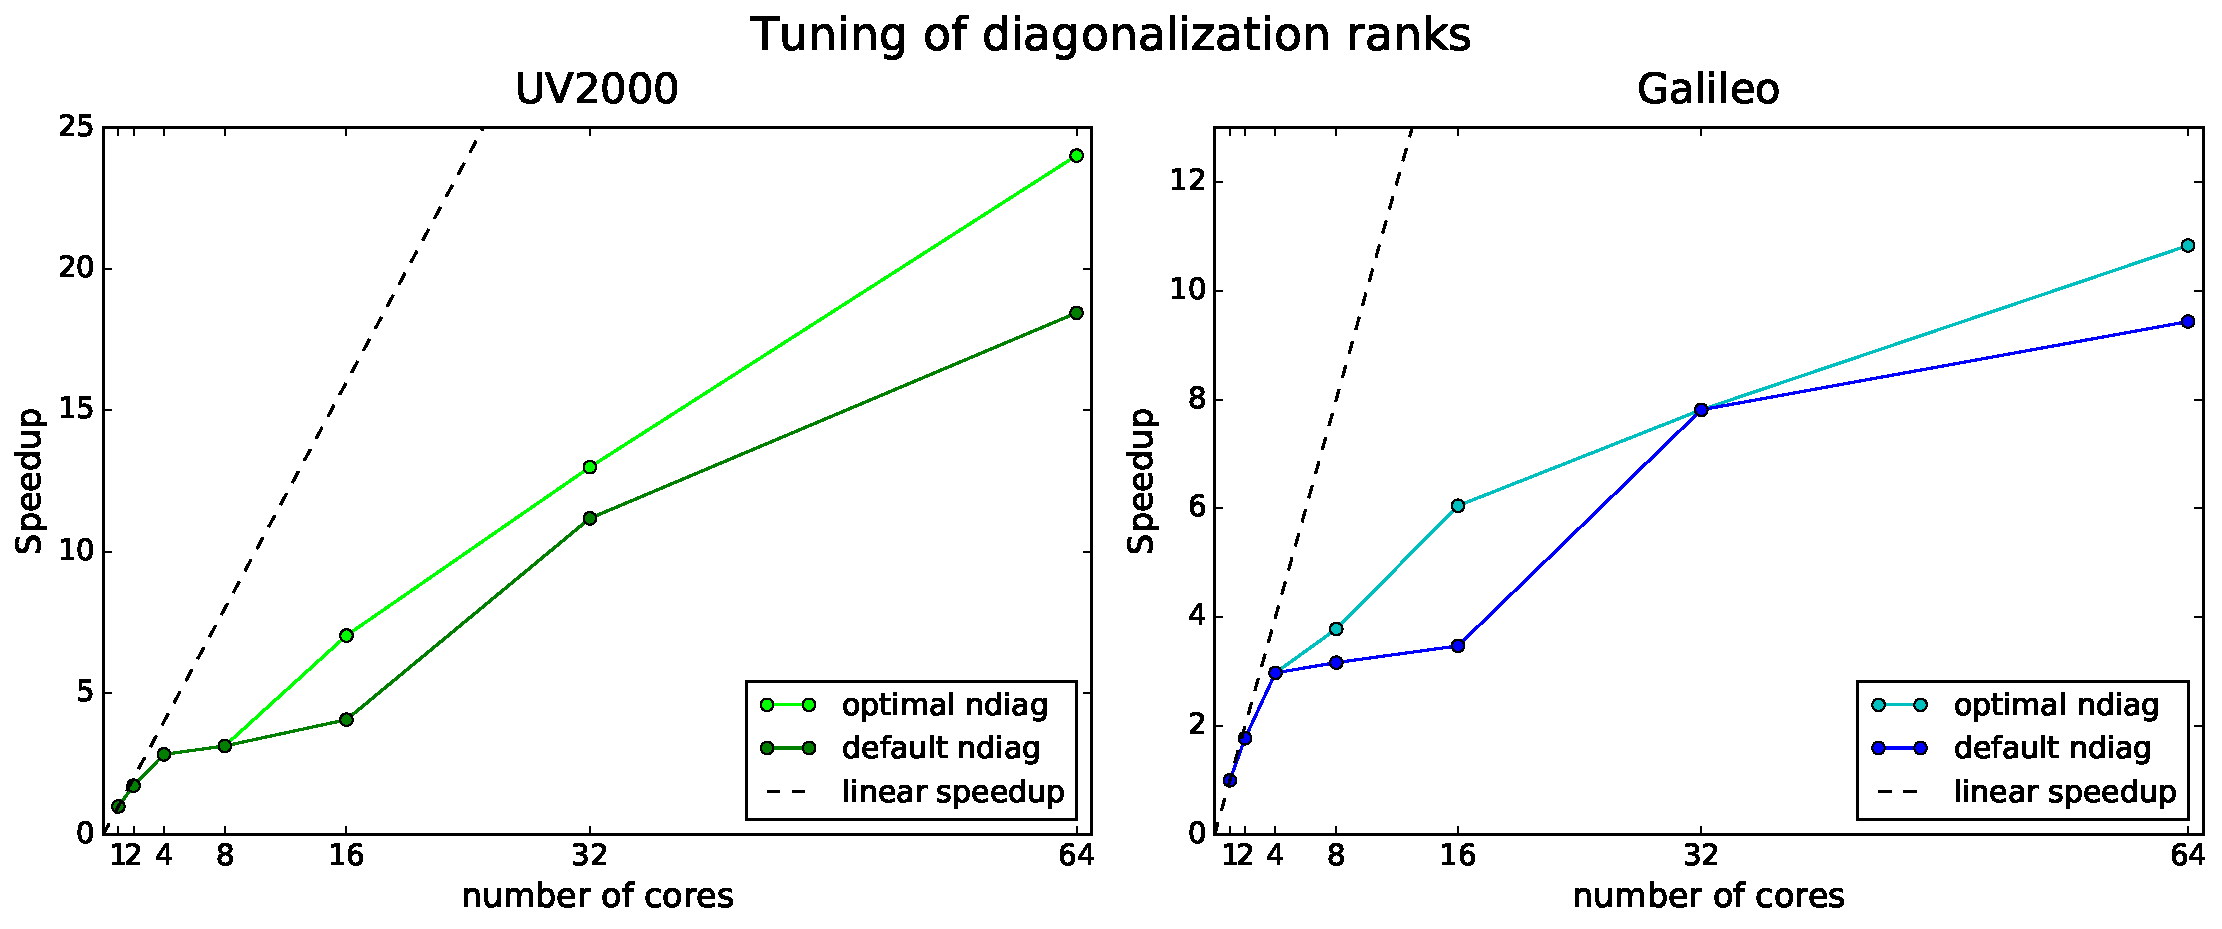
\includegraphics[width=1.2\linewidth]{ndiag_speedup.pdf}	}
	\caption{PWscf's speedup comparison between default runs and runs that optimizes the number of diagonalization processors (fixed number of iterations).}
	\label{fig:ndiagSpeedup}
\end{figure}


\newpage
\begin{center}
\begin{framed}
	What is the overall behavior of Quantum ESPRESSO in function of the scale of the physical system?
\end{framed}
\end{center}



In the following we report PWscf's speedup on a series of different systems\footnote{Non optimized runs only.}, which were chosen to span the common dimensions of nanocrystalline systems.

\begin{itemize}
	\item As a ``\textit{small}" system we used the \CO system (see figure \ref{fig:conclCo3} and appendix \ref{app:Co3}).
	\item As a ``\textit{medium-small}" system we used the AUSURF112 PRACE system\cite{prace} (see figure \ref{fig:conclAusurf} appendix \ref{app:Ausurf112}).
	\item We consider the TiO\textsubscript{2} a ``\textit{medium-large}" system (see figure \ref{fig:conclTitania}).
	\item An organic OLED crystal was used to simulate a ``\textit{large}" system (see figure \ref{fig:conclOled} and appendix \ref{app:Oled}).
\end{itemize}

\begin{figure}[hhh!]
\centerline{ 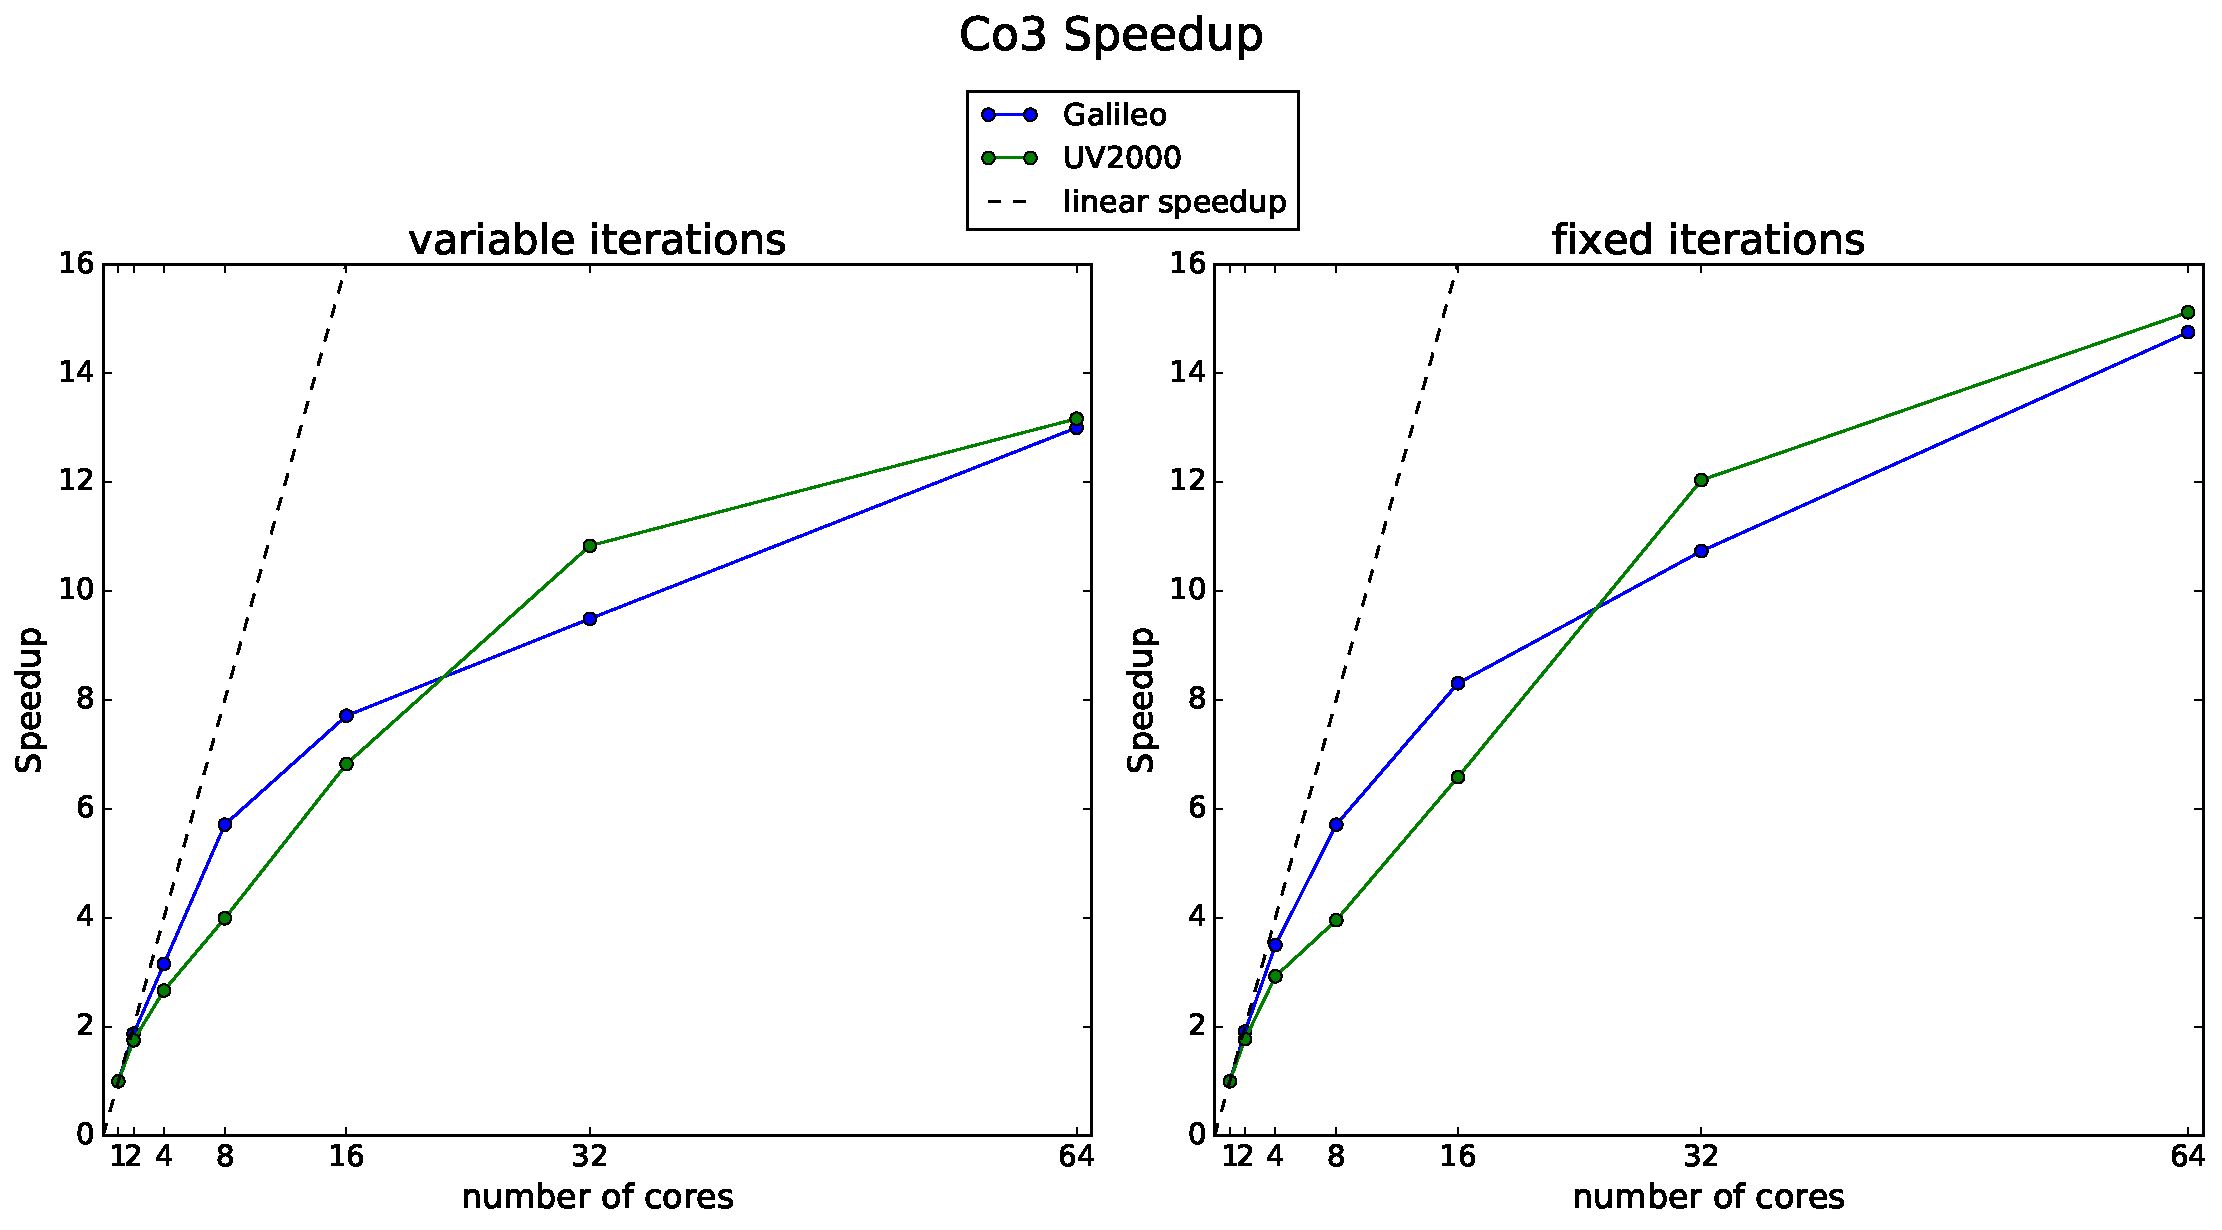
\includegraphics[width=1.\linewidth]{concl_co3.pdf}	}
	\caption{PWscf's speedup for a ``\textit{small}" scale \CO system.}
	\label{fig:conclCo3}
\end{figure}


\begin{figure}[hhh!]
\centerline{ 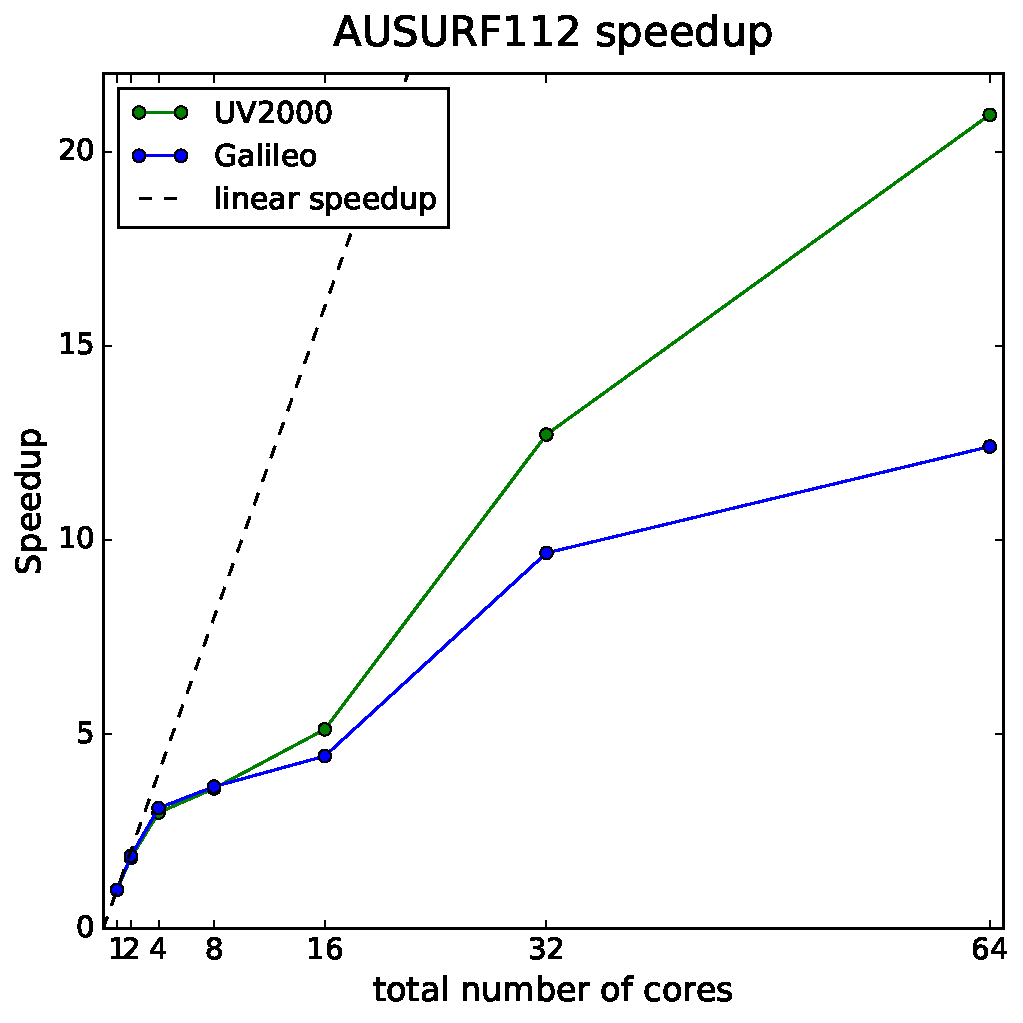
\includegraphics[width=0.5\linewidth]{concl_ausurf.pdf}	}
	\caption{PWscf's speedup for a ``\textit{medium-small}" scale AUSURF system.}
	\label{fig:conclAusurf}
\end{figure}
\newpage


\begin{figure}[hhh!]
\centerline{ 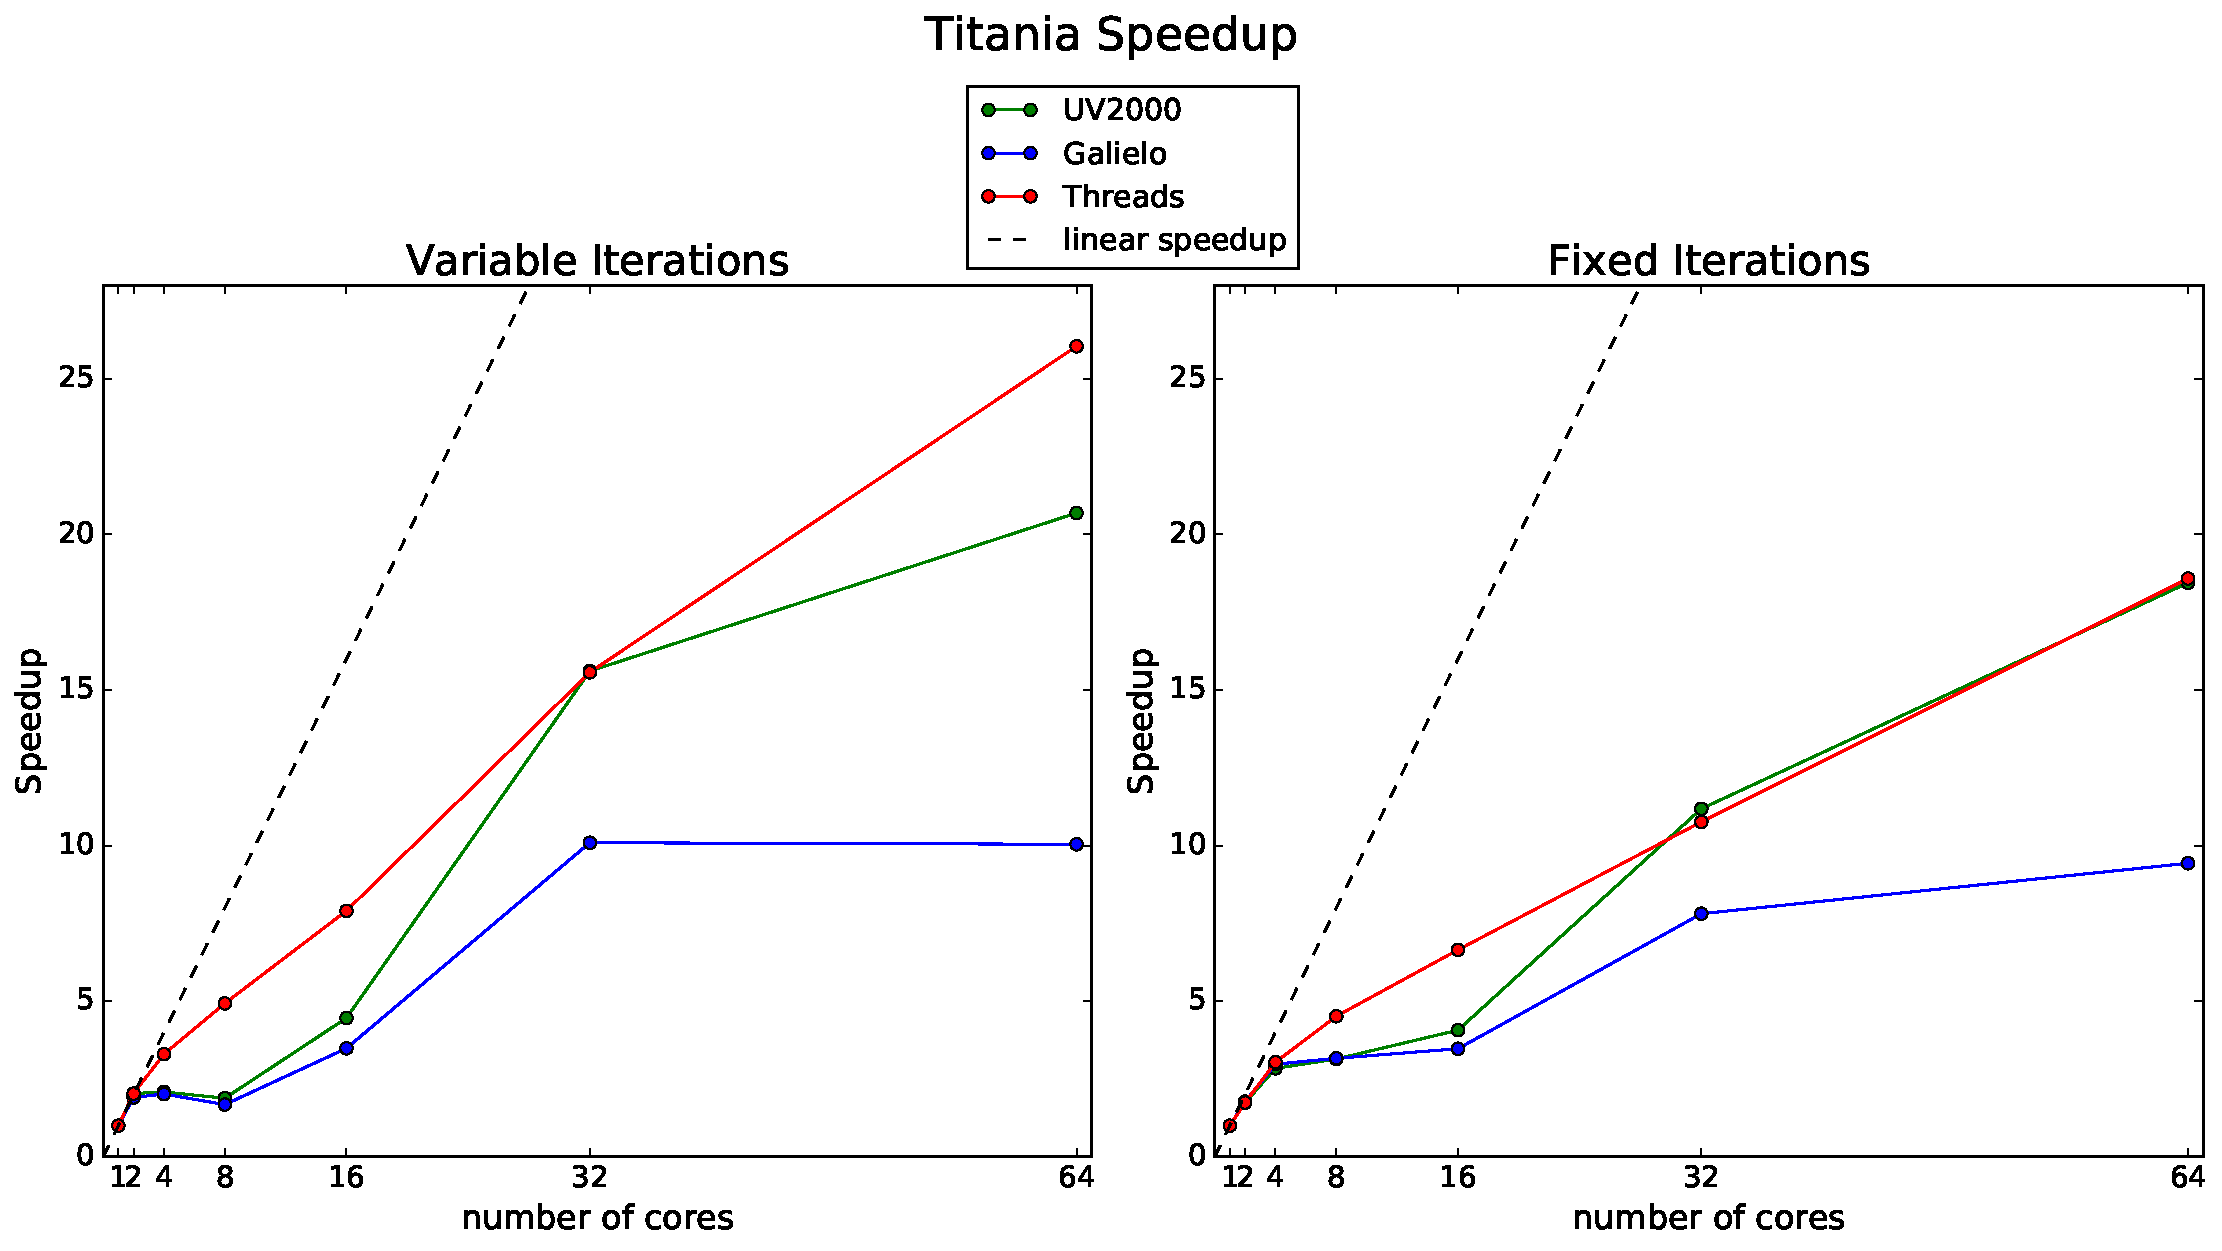
\includegraphics[width=1.\linewidth]{concl_titania.pdf}	}
	\caption{PWscf's speedup for a ``\textit{medium-large}" scale TiO\textsubscript{2} system.}
	\label{fig:conclTitania}
\end{figure}

\newpage
\begin{figure}[hhh!]
\centerline{ 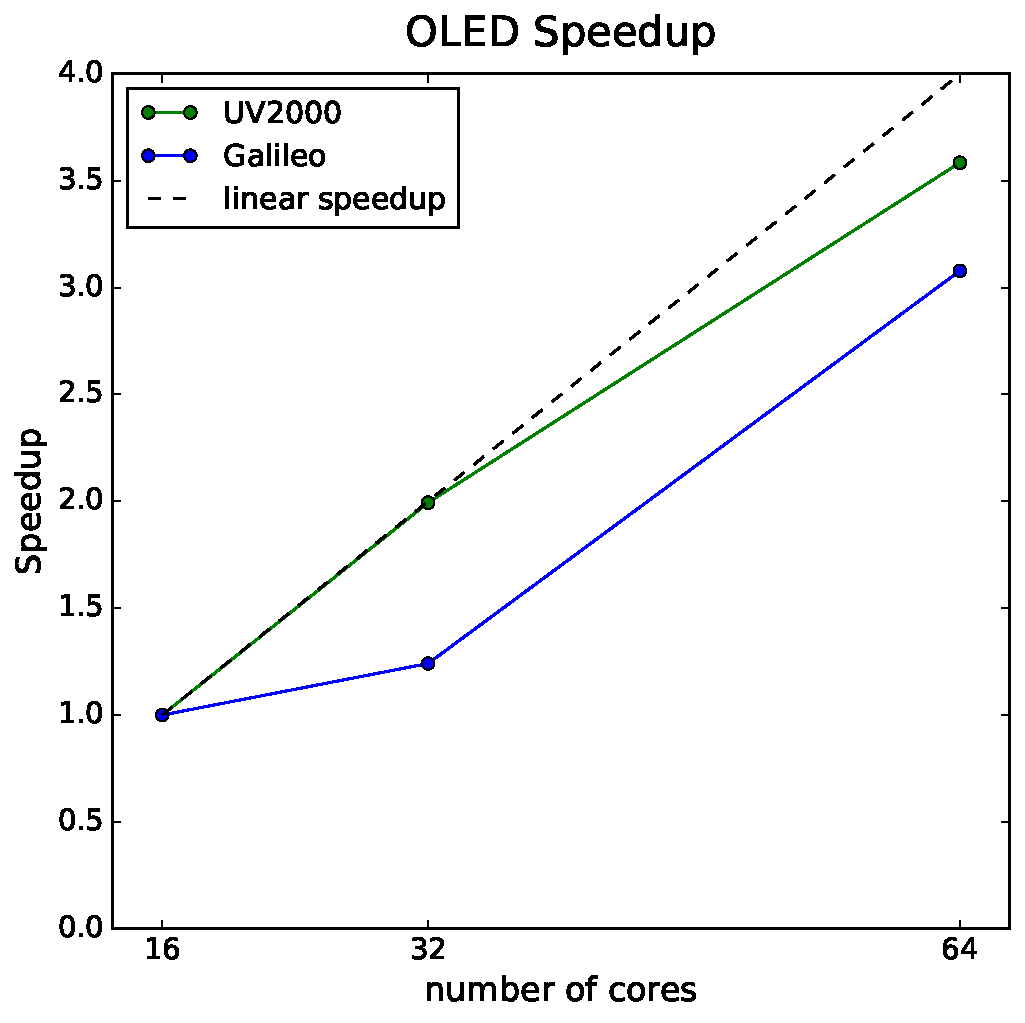
\includegraphics[width=0.5\linewidth]{concl_oled.pdf}	}
	\caption{PWscf's speedup for a ``\textit{large}" scale OLED system.}
	\label{fig:conclOled}
\end{figure}


Starting from the \CO system we can see that on \textit{small} scale systems there is only a slight advantage of the UV2000, which is limited to scaling and not to CPU time.


The fact that the scalability plots of AUSURF (figure \ref{fig:conclAusurf}) and Titania (figure \ref{fig:conclTitania}) are incredibly alike (AUSURF was performed only at fixed number of iterations), suggests that the UV2000 is particularly suited to simulate this kind of systems; 
where more than a hundred atoms with large empty portions of the supercell are present.

We can say that when the system starts to increase in size, the UV2000 has a noticeable advantage compared to Galileo.
Note that at 32 and 64 cores also the CPU time of the UV2000 is lower than Galileo's one, meaning that the advantage is both on scaling and overall performance.

We can impute this to the increasing relevance of matrix diagonalization over matrix evaluation\footnote{We have seen that \texttt{h\_psi} speedup difference is less impac	ting that \texttt{cdiaghg}'s one.} and the subsequent necessity of high performance communication( see above and \cite{QE2}).


The advantage (in time and scalability) is maintained also on particularly large and complex systems, like OLED crystals (figure \ref{fig:conclOled}), but not increased; suggesting some sort of saturation.
Unfortunately to investigate further this aspect, larger resources are needed, three points on a plot seems not to be sufficient.
Consider also that, unfortunately, the time at our disposal was insufficient\footnote{Actually it was terminated.} to produce more precise profiling metrics (i.e. using \texttt{scorep}).

\newpage
\section{Discussion and Conclusion}\label{sec:conclusions}

The aim of this work was to find tuning strategies to optimize \QE (QE) performances on different computational architectures.

In order to do it properly a great amount of preparatory work was performed.

First we studied the theoretical foundations of ab initio calculations, familiarizing with the first, and nowadays still popular, self consistent field (SCF) method: the Hartree-Fock (HF) method.
We studied its critical features and mechanisms.

Starting from the computational limits of HF method we introduced the density functional theory (DFT), which shifts the problem from finding exact electronic orbitals to finding the ground state electronic density.
We highlighted how, in this framework, the variational approach translates into a new SCF formulation, and how the choice of plane waves as a basis set changes the computational dimensionality of the problem.
A comparison between HF and DFT was performed to underline how this new theory overcomes previous computational limits.

Only at this point we were able to fully understand how SCF DFT is translated into real world algorithms inside QE.
We studied how each step of the SCF cycle is implemented, what algorithm are used to perform the calculations, what are the subroutines implementing each step of the SCF cycle and what are the computational complexities of each relevant subroutine.

Once the mechanics of QE were clear, we could concentrate on an analysis of the two computational architectures studied:
a classic multicomputer cluster (CINECAS's Galileo cluster) and a shared memory NUMA multicomputer (the Sgi UV2000).

We underlined all the differences between the two systems which mainly lies in the presence or absence of global shared memory and the interconnect technology adopted. 
We performed also a series of introductory tests to find the main factors that could bias our measurements and we reported the methods to minimize them.

We also outlined all the critical aspects that rises when trying to evaluate the performance of an SCF algorithm; namely the numerical instability associated both to the number of iterations needed to reach self consistency and the differences in execution time of each iterative step.
We also performed an in depth analysis of where and how interprocess communication (MPI) is performed within the code.

Given the knowledge accumulated, we finally had all the tools to properly tune the computational architecture.

Our results can be structured in two main categories : architecture independent tuning and architecture dependent tuning.

For architecture independent tuning we found that, in contrast to what reported in literature, second level parallelization performed within the multi-threading paradigm (OpenMP) can have a strong positive impact when a relatively low number of cores is employed.
The use of threads in this framework achieves a better numerical stability lowering the number of SCF iterations step needed to reach self consistency and improves sensibly the performance of matrix diagonalization, which constitutes the major computational bottleneck.
This result can be of great interest for hight throughput computing scenarios (modeling of hundreds of dimensionally similar systems) or when shared computational resources are overloaded and low parallelized runs performed locally can lead to sooner results than high parallelized jobs waiting to be executed on massive, nevertheless overcrowded, shared clusters.

With an architecture dependent perspective we found that the UV2000 is more suited to perform calculations of ``\textit{medium size}" systems (one hundred to two hundreds atoms in surface configuration) while Galileo cluster has a general advantage on ``\textit{small size}" systems (approximately fifty atoms).
We have also performed a brief test with a ``\textit{large}" organic OLED crystal confirming that the advantage of the UV2000 is still present but not increased compared to medium size systems.

We also found that UV2000's performances overtakes Galileo's ones when two or more Galileo's cluster nodes are employed in the calculations.
This suggests a more efficient handling of the interprocess communication performed by the UV2000, this impression was confirmed by the profiling metrics obtained and by comparing the behavior of QE's communication routines.

We also found that matrix diagonalization still constitutes a major bottleneck above the 8 core landmark and we found that the methods to optimize its performances where very different between the two architectures.

For Galileo cluster the best results were achieved reducing the number of cores dedicated to diagonalization to fit the maximum number of cores hosted by a single cluster node (a total of sixteen), which is consistent to what is suggested in literature.

On the contrary, for the UV2000 the best results are obtained by increasing as much as possible the cores dedicated to diagonalization.
Since distributed matrix diagonalization performs high volume communication, shared memory architectures proves to be more efficient for this kind of calculations.

To conclude this work we propose in figure \ref{fig:conclFinalComparison}	two plots that summarizes the improvements obtained by applying the tuning strategies discussed above.

\begin{figure}[hhh!]
\centerline{ 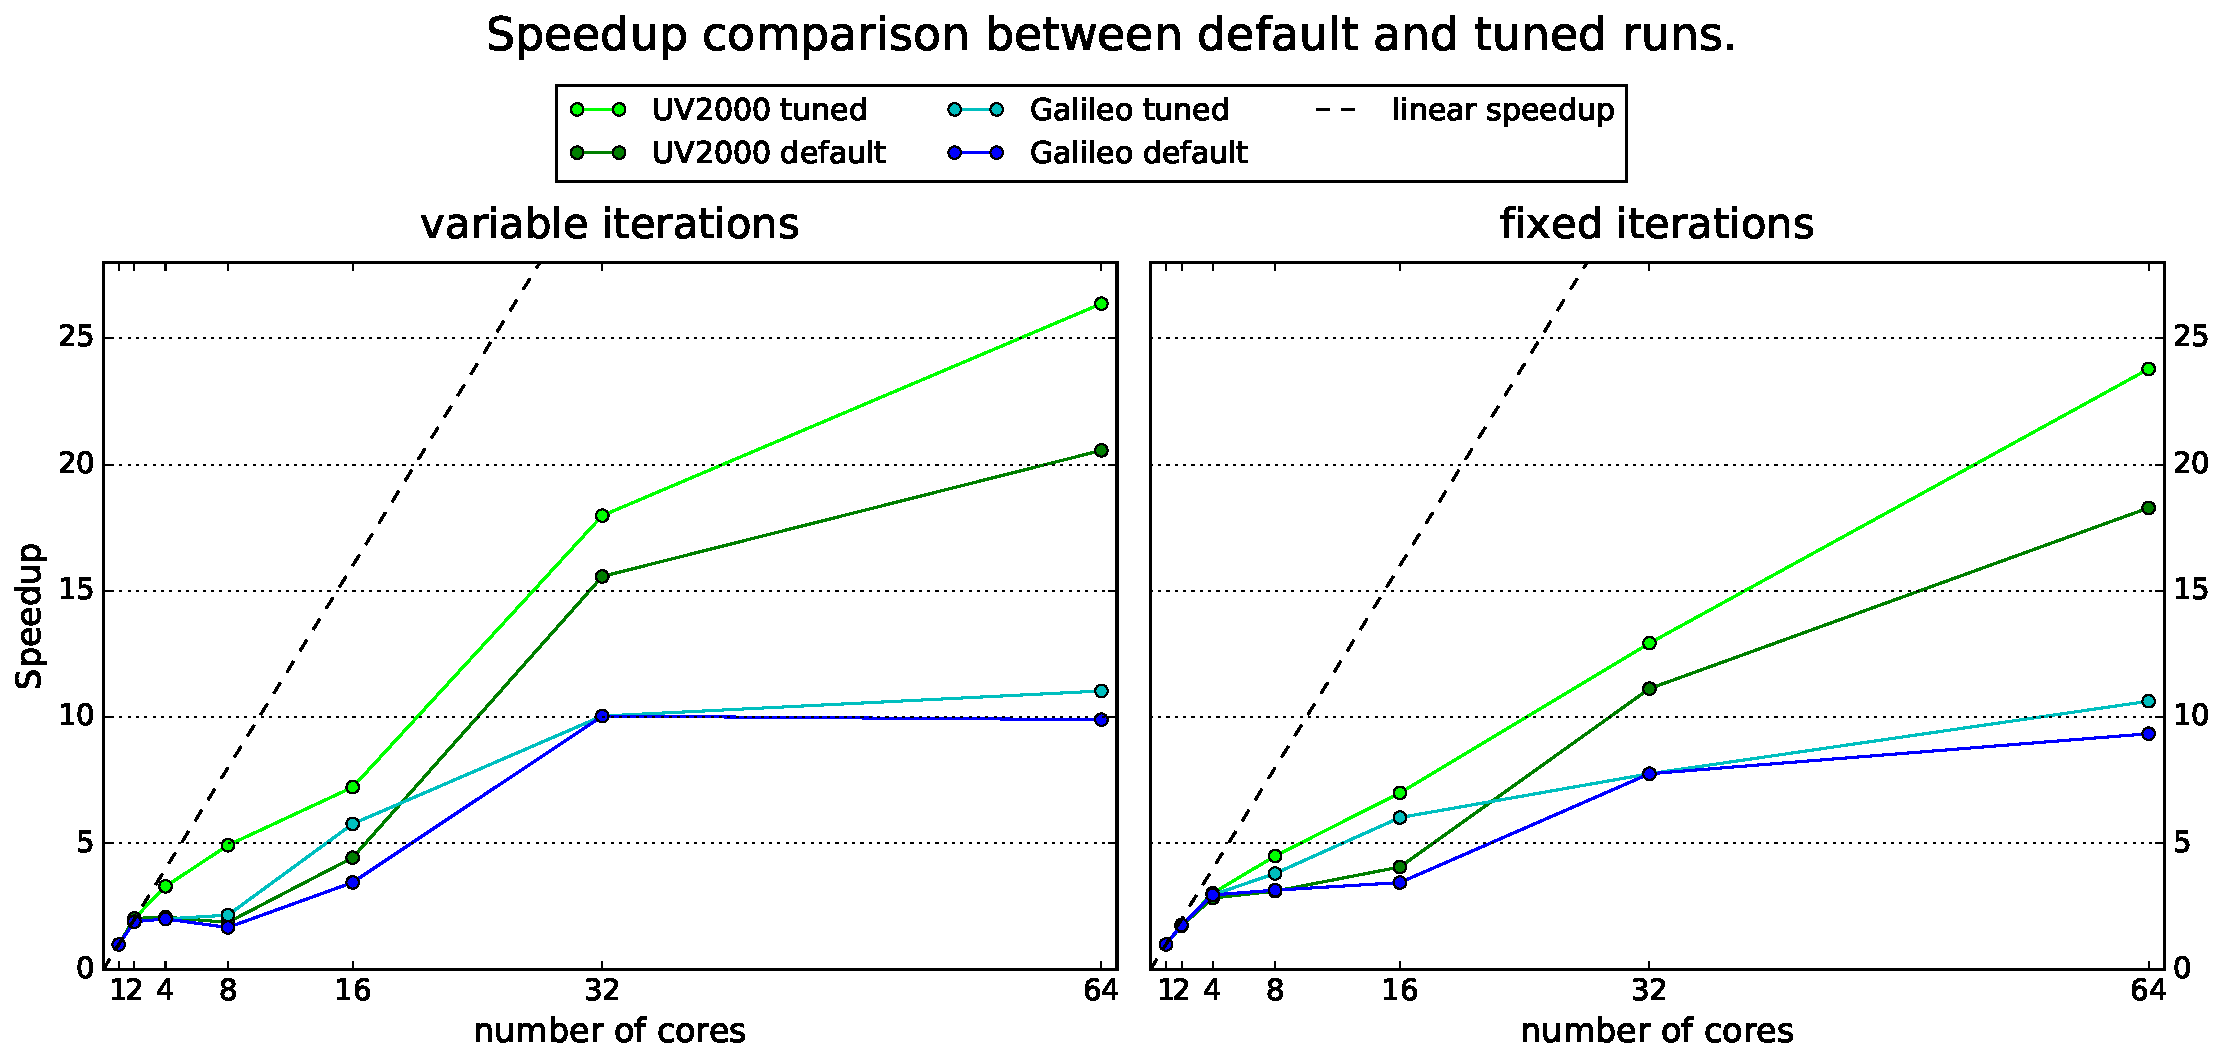
\includegraphics[width=1.2\linewidth]{concl_final_comparison.pdf}	}
	\caption{Tuned runs were performed applying the rules exposed in section \ref{sec:results}.}
	\label{fig:conclFinalComparison}
\end{figure}

We can see that our tuning strategies have a positive impact both at fixed and variable iterations.

Another important thing to note is that on the right plot we have finally reached linear scaling after the one node limit is passed and this was only possible with proper tuning strategies.

Also note that at 16 cores a properly tuned run on the Galileo cluster can still outscore a default run on the UV2000, but when more than one cluster node is needed the UV2000 have a sensible lead.

The fact that the multiprocessor system outscores the multicomputer system especially at variable number of iterations (i.e. until self-consistency is reached) should motivate a certain interest in investigating further how ab initio calculations can benefit from this kind of computational architecture.


\newpage
\subsection{Outlooks}

This work have outlined some interesting aspects of \QE SCF DFT implementation.

\paragraph{Numerical (in)stability} We have seen in section \ref{sec:resCriticalComponents} that the time required to complete a single SCF iteration step varies considerably from step to step.
By investigating further the distribution of the CPU time of each step, no particular trend or distribution can be inferred.
We think that a further analysis of the implementation can lead to better results an increase the efficiency of the cycle.

Also the wide difference in the number of iterations needed to reach self-consistency while changing the number of total cores is somewhat of an unexpected behavior. 
Note that the variation of the number of cores dedicated to diagonalization do not affects SCF dynamics, the energies obtained at the end of each step are exactly the same, regardless of the number of cores implied.
This suggests that the instability must lies in the evaluation of the Hamiltonian and that better convergence performance can still be achieved.

One possible approach to narrow the causes could be to variate independently the size of the various MPI communicators available in QE and measure how the number of iterations changes.

\paragraph{Multithreading} The other unexpected result was that the use of threads could enhance performance, especially at variable iterations. 
It is interesting to note that modern HPC processors will host a constantly greater number of cores, embedding the technologies developed for Intel Xeon Phi accelerators inside the main board chipset (the so-called MIC architecture).
How this new technology is going to impact on QE performances is hard to predict beforehand but it will be interesting to see if the trade-off between an FFT performance loss and an linear algebra performance boost will still pay on such scale.


\paragraph{Matrix multiplication algorithms} In section \ref{sec:resArchDependent} section we have stated that QE needs a $n*n$ grid of cores (where $n$ is a natural number) to perform a full memory distributed matrix multiplication.
This limitation can leave a considerable number of cores unused.
It would be interesting to see if the use of different algorithms without this limitation can positively impact on QE performances, especially on the UV2000 where increasing the number of diagonalization cores seems only to enhance the performance. 
For example the SUMMA (Scalable Universal Matrix Multiplication Algorithm) algorithm doesn't require an $n*n$ grid to work.

We have also seen in section \ref{sec:resArchDependent} that the default number of diagonalization cores was the optimal one only when 32 total cores where used on Galileo. 
In previous version of QE the diagonalization of a test matrix was performed during the initialization with different numbers of diagonalization cores, in order to find the optimal one.
The approach was deprecated because considered unreliable.

In the current release the size of the diagonalization communicator is calculated in function of the number of total cores employed. 
Maybe an approach that takes under consideration also the dimension of the system could lead to a better guess.


\paragraph{Increasing the resources} It would be interesting to see for how long the linear scaling achieved in figure \ref{fig:conclFinalComparison} will be maintained and if the advantages of the UV2000 will still stand on bigger nanocrystals and on different regions of the core's scale.

Also the coupling of the UV2000 with the GPU accellerators can lead to interesting results.


\paragraph{Predictive analytics for better tuning} How many \QE calculations are performed every day? It sure is an interesting amount of profiling metrics, generated for free by the PWscf profiler. 
In this work we have seen that these metrics are reliable and can lead to efficient tuning strategies.
We have also seen that such strategies varies strongly with the computational architecture and the size and type of the physical system.
In my opinion it could be incredibly interesting to harvest and accumulate all those metrics along with systems configurations and computational architecture specifications to see if it is possible to find trends and algorithms to predict better tuning parameters beforehand.
It will require for sure a great amount of collaboration within the community, a solid infrastructure and great analytical capabilities, but I hardly doubt that the costs will be higher than a couple of racks of the next top 500 supercomputer.



\begin{appendices}

\newpage
\section{Makefiles} \label{app:makefiles}
\subsection{Galielo}
\lstinputlisting[language=make,basicstyle=\tiny ,breaklines=true,tabsize=2]{media/listings/make.sys.galileo}

\newpage
\subsection{UV2000}
\lstinputlisting[language=make,basicstyle=\tiny ,breaklines=true,tabsize=2]{media/listings/make.sys.numa}


\newpage
\section{Iterations Dynamic} \label{app:IterationDynamic}

Various metrics relative to single iterations and their behavior in function of the number of cores employed.

\begin{figure}[hhh!]
	\centerline{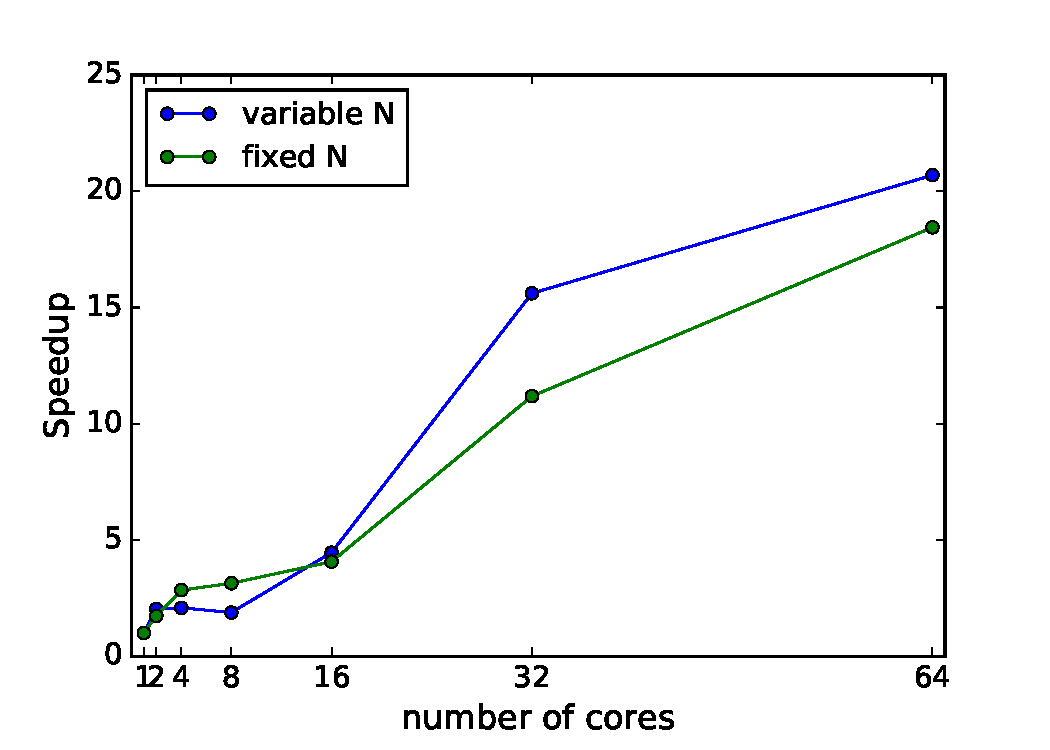
\includegraphics[width=0.6\linewidth]{fixed_vs_variable_speedup.pdf}}
	\caption{ Speedup comparison between fixed and variable iterations.
	}
	\label{fig:fixedvsvariablespeedup}
\end{figure}

\newpage
\begin{figure}[hhh!]
	\centerline{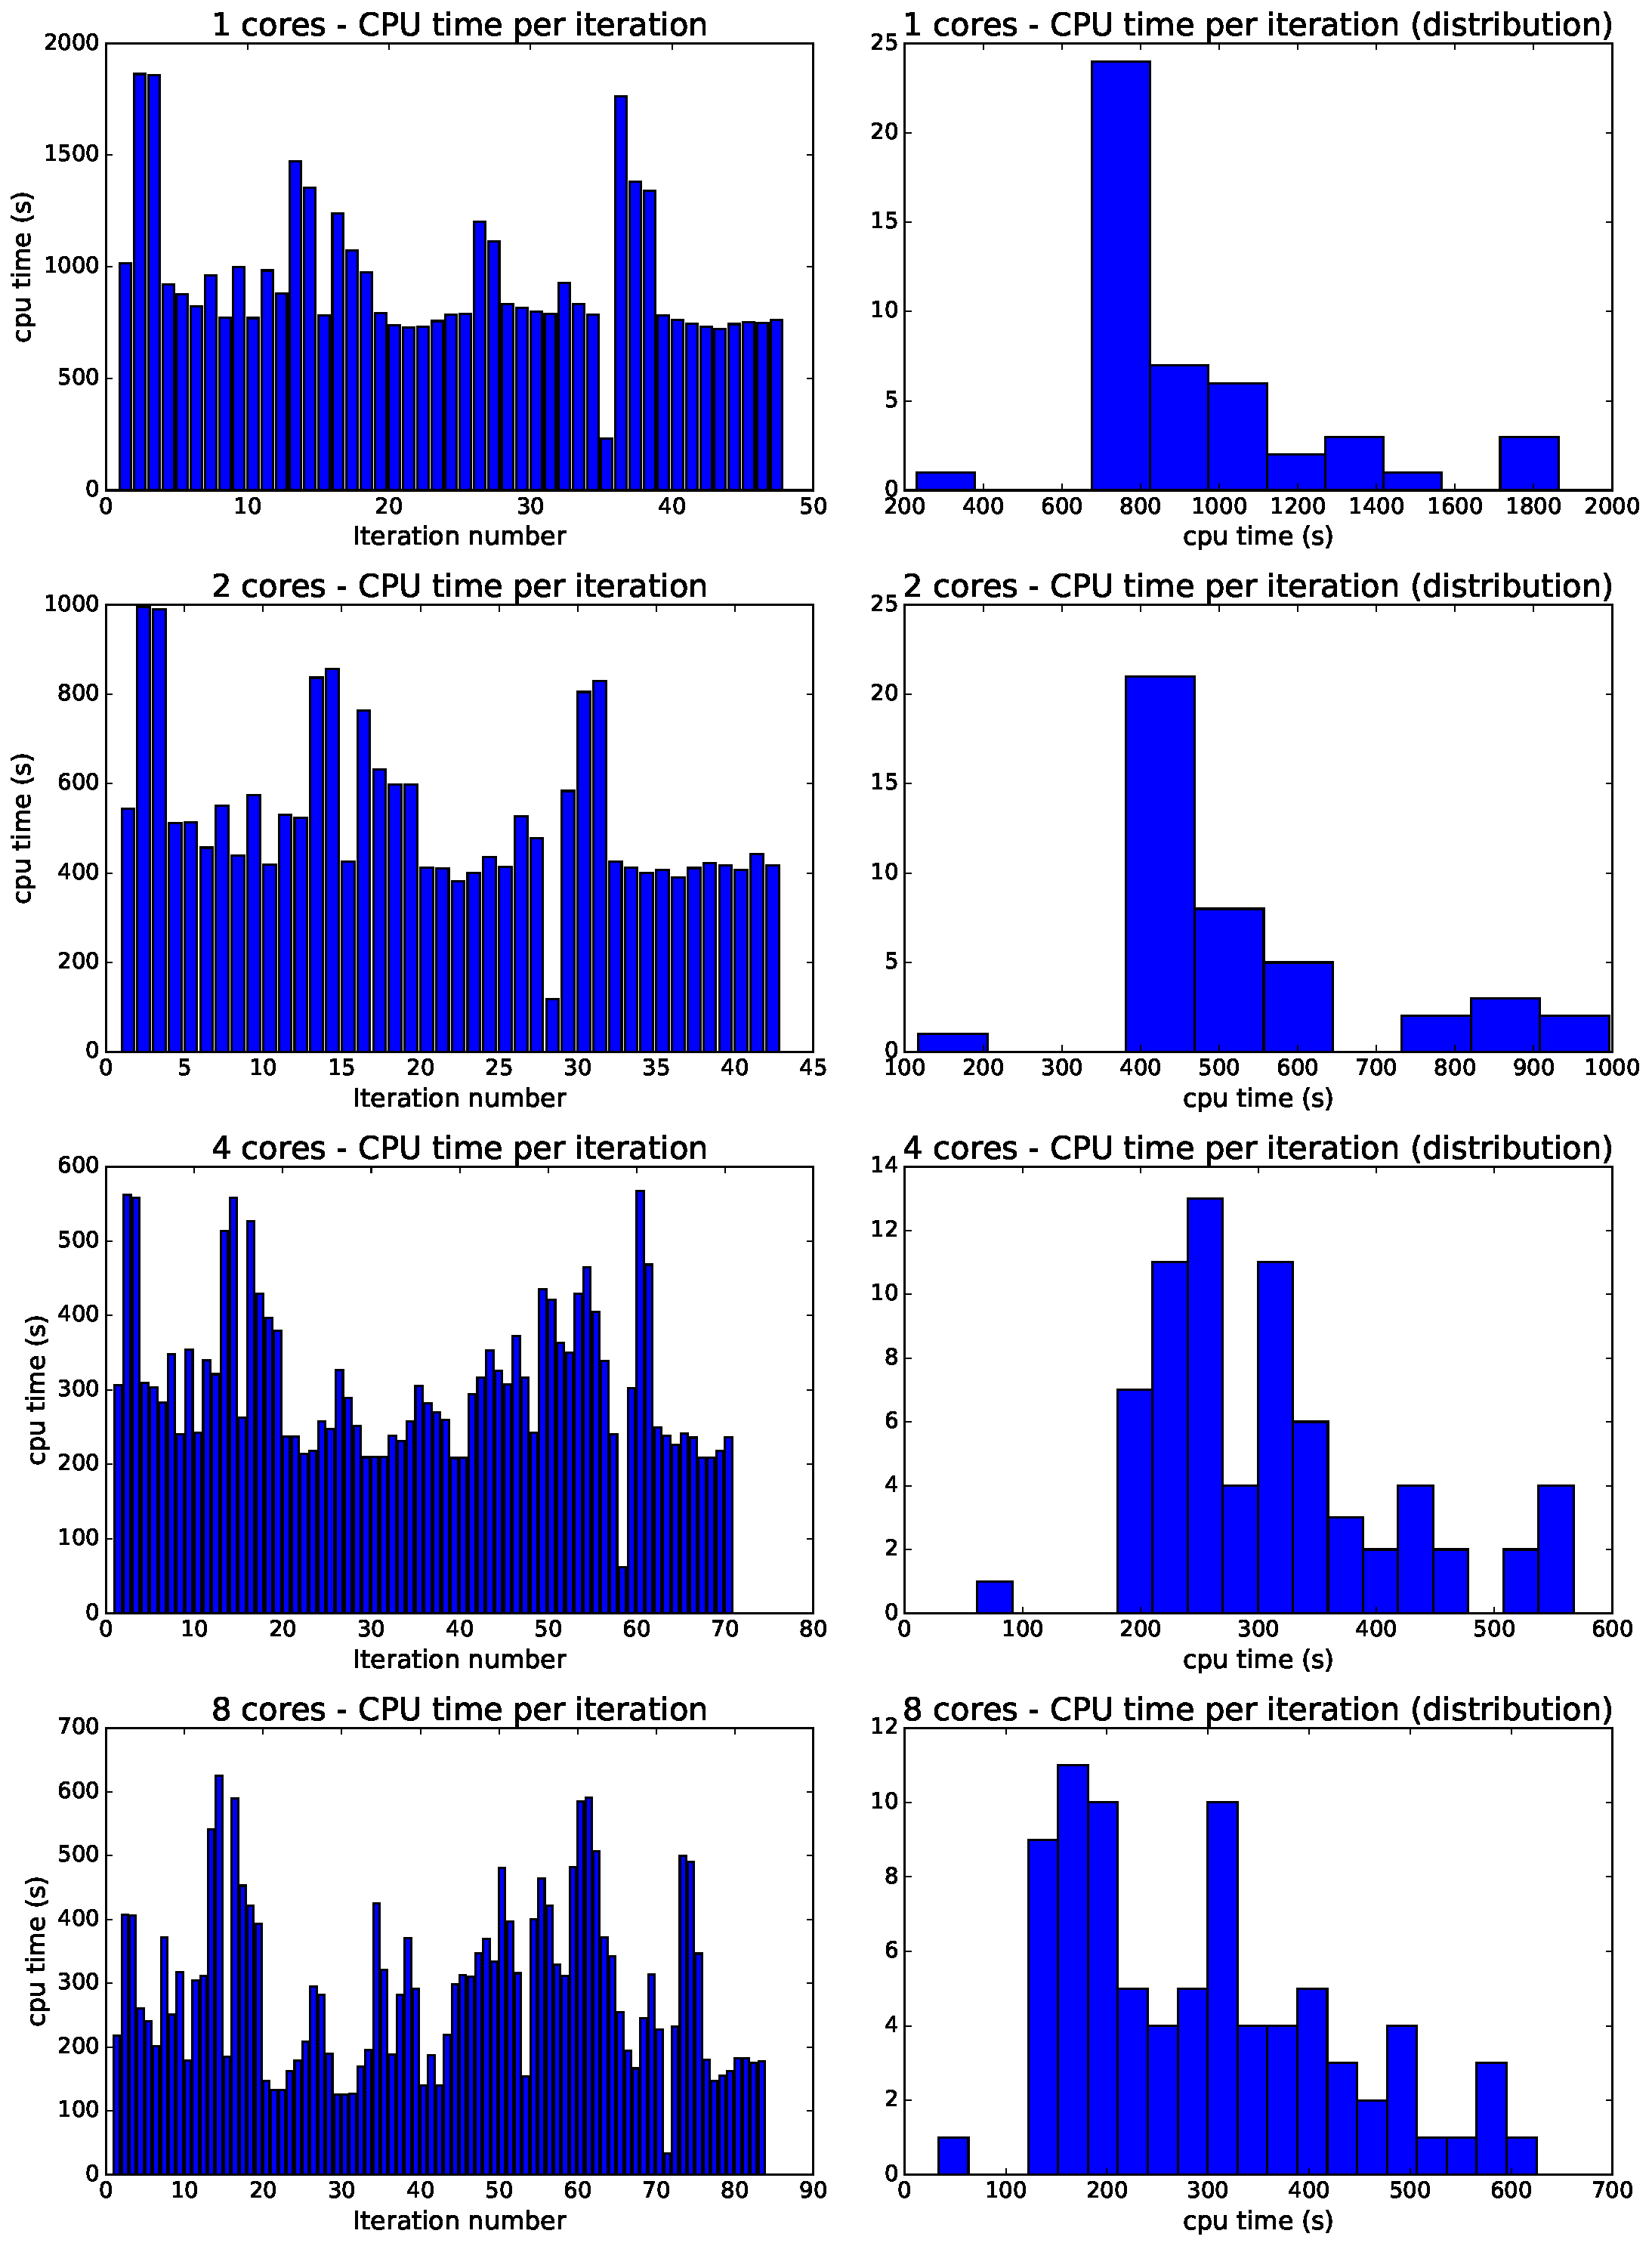
\includegraphics[width=1.\linewidth]{app_iterations_distro1.pdf}}
	\caption{ Iteration CPU time statistics
	}
	\label{fig:fixedvsvariablespeedup}
\end{figure}

\newpage
\begin{figure}[hhh!]
	\centerline{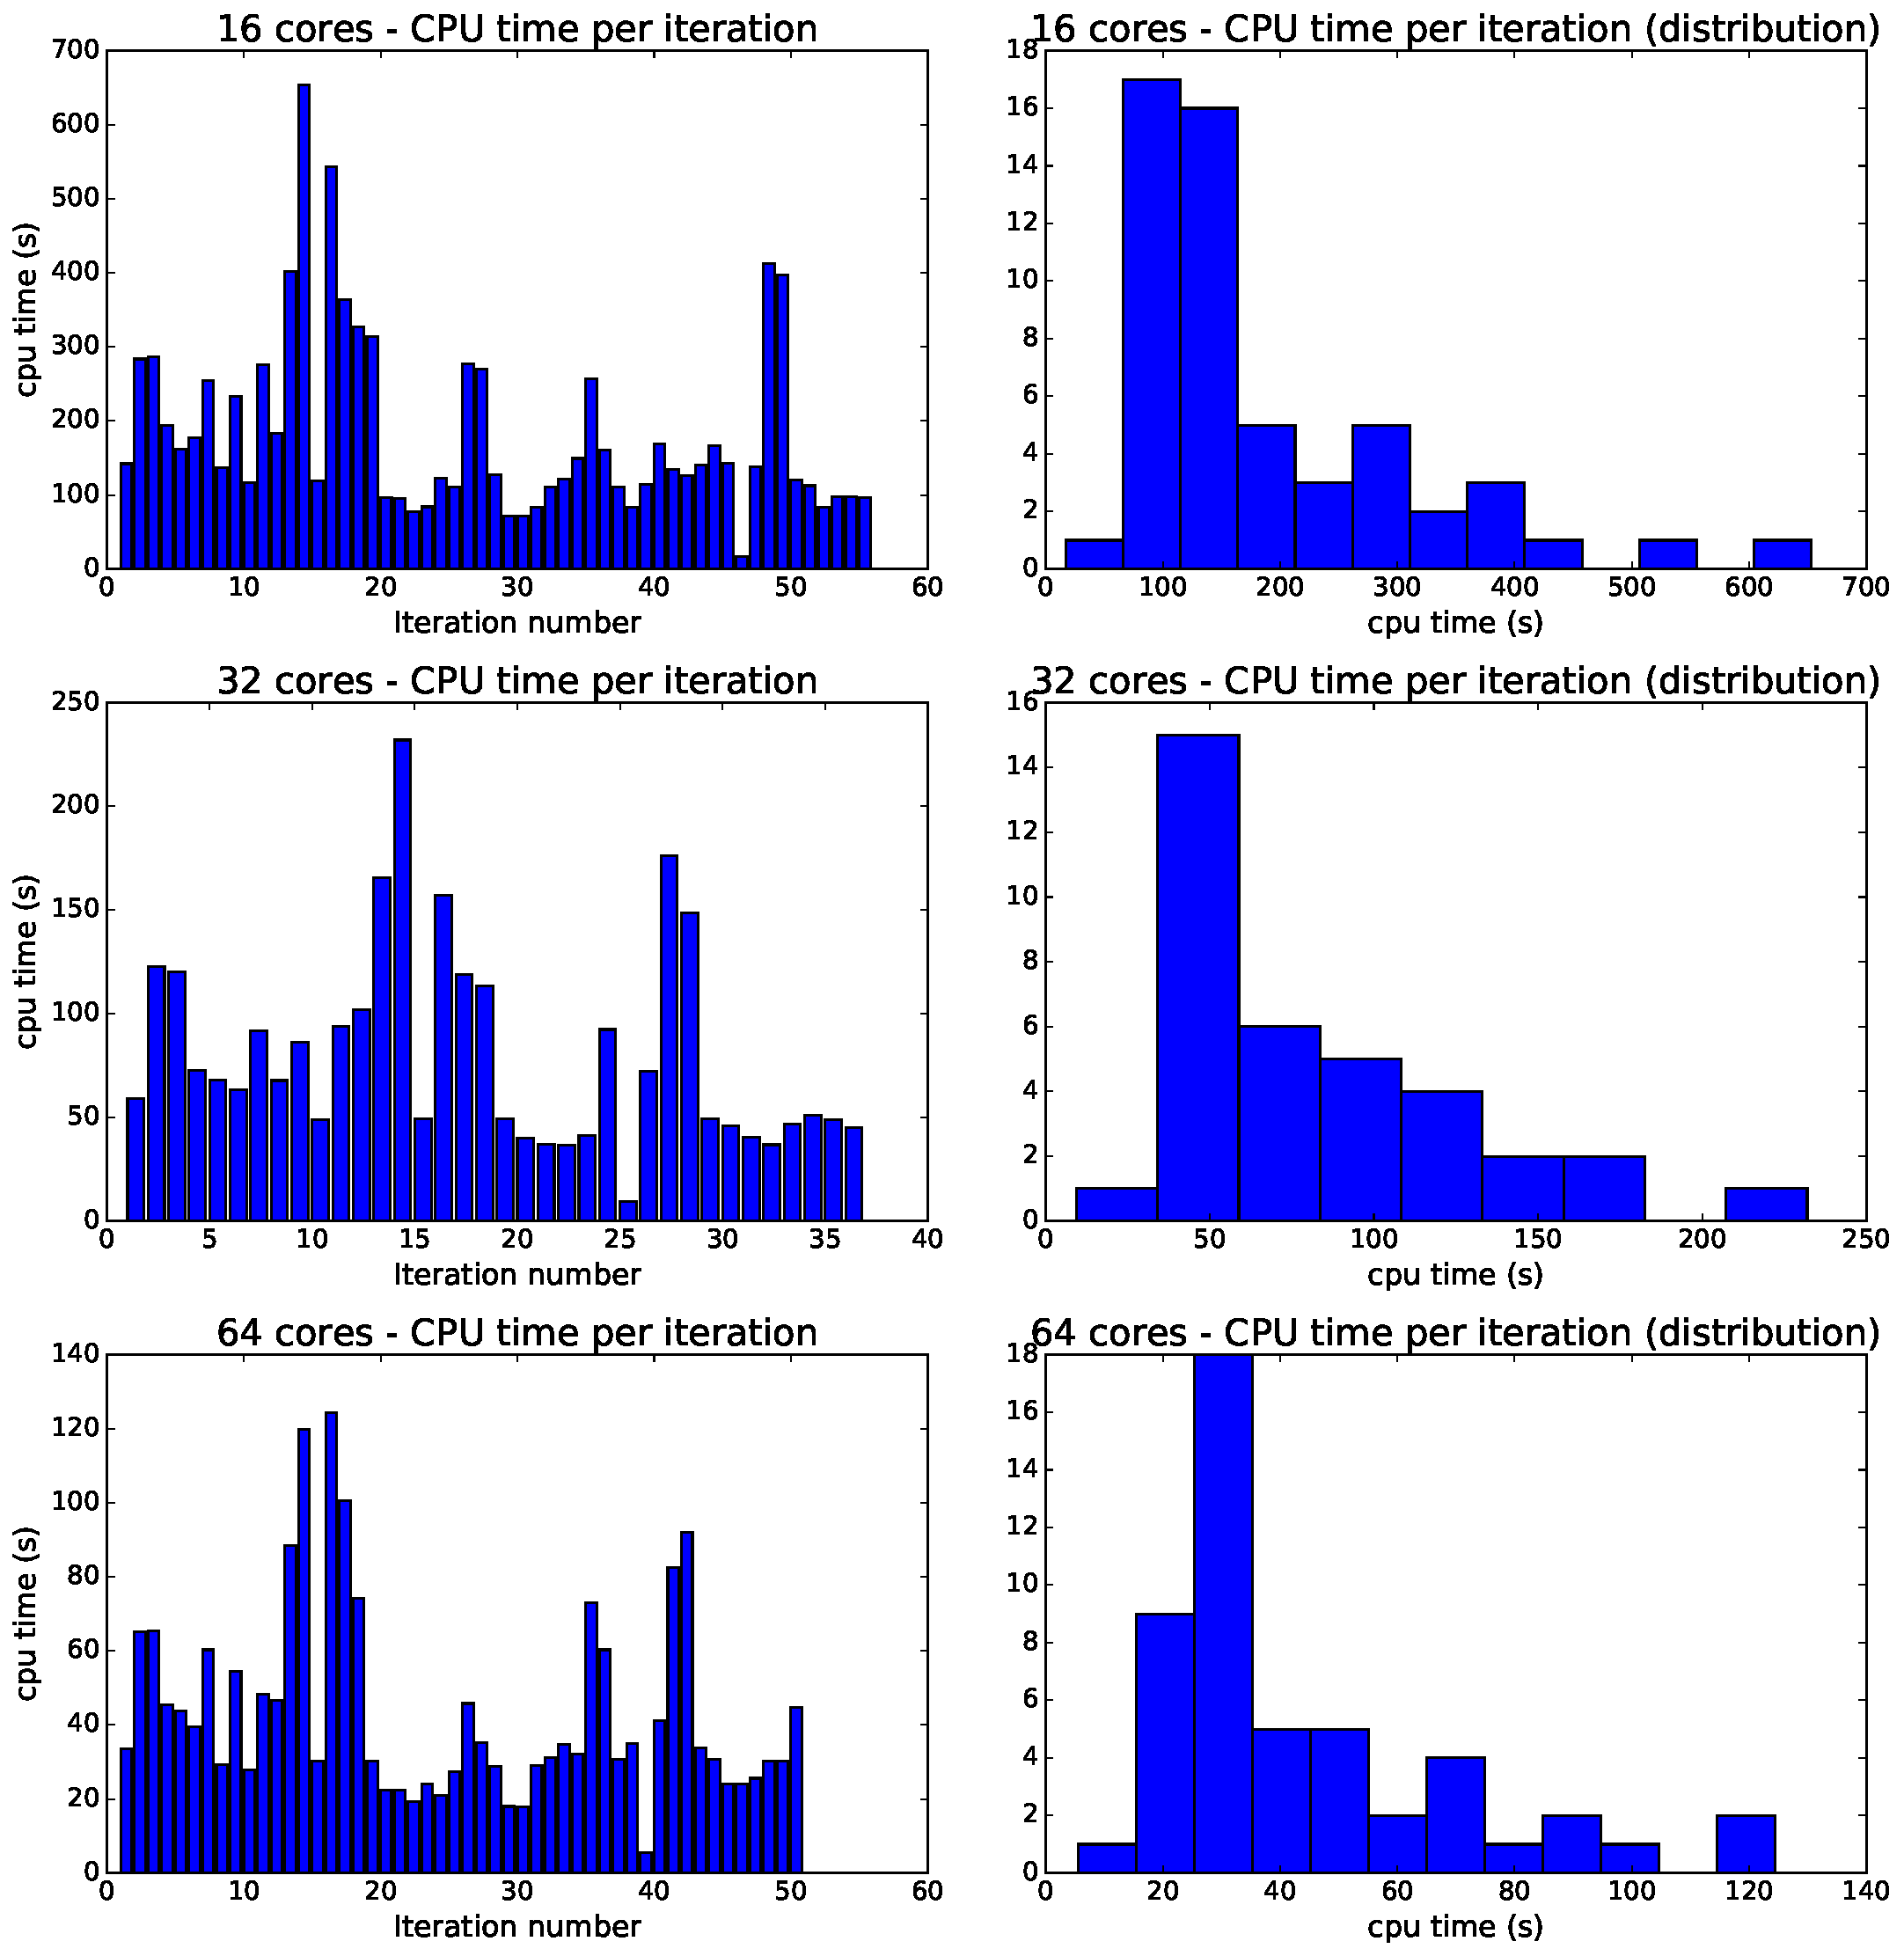
\includegraphics[width=1.\linewidth]{app_iterations_distro2.pdf}}
	\caption{ Iteration CPU time statistics
	}
	\label{fig:fixedvsvariablespeedup}
\end{figure}


\newpage
\section{Threads}\label{app:Threads}

In absence of a run at fixed number of iterations we have performed a rescaling of the CPU time and WALL time of all the functions.
To rescale factor was calculated obtaining the CPU time at the end of the 20\textsuperscript{th} iteration ( this information can bee extracted form PWscf output, see \cite{qetools}) and dividing it by the total PWscf's CPU time.

\begin{figure}[hhh!]
	\centerline{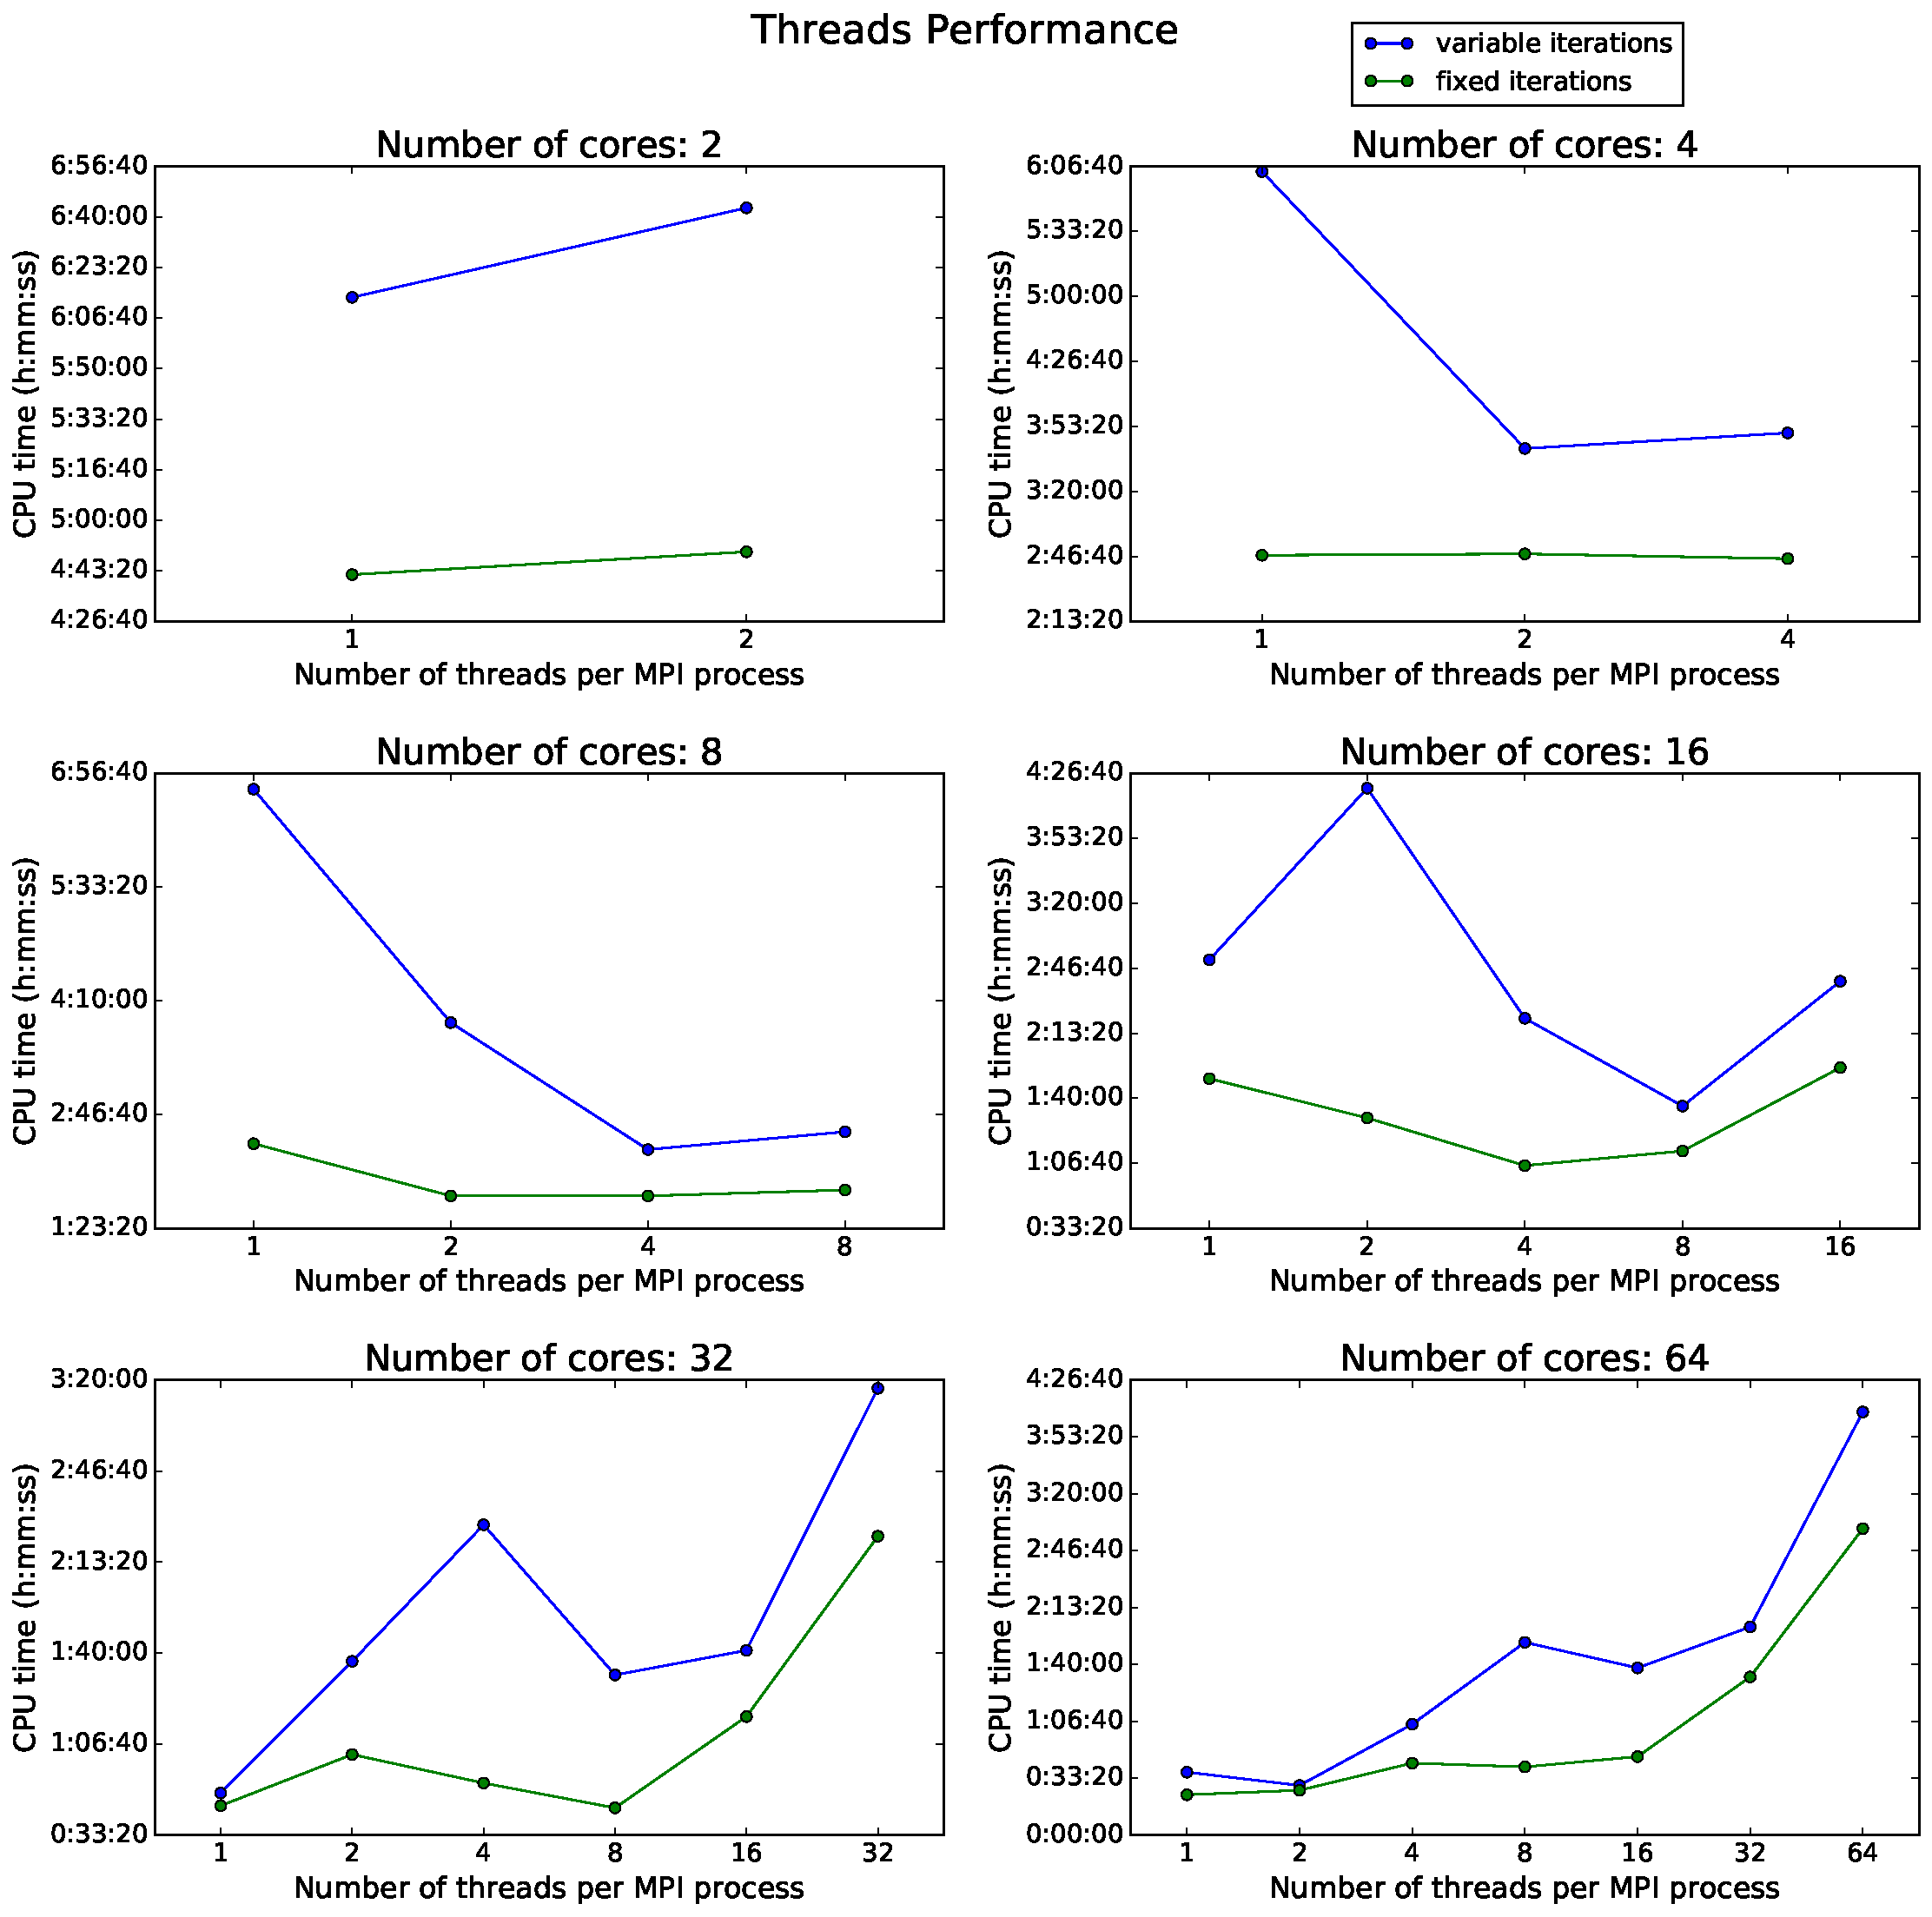
\includegraphics[width=\linewidth]{A_threads.pdf}}
	\caption{ PWscf's CPU time using different number of threads (\texttt{OMP\_NUM\_THREADS}).
	\\The number of cores is the total number of occupied cores when all threads are in use.
	\\The number of MPI process is $ N_{MPI} = N_{cores} / N_{threads} $ .}
	\label{fig:A_threads}
\end{figure}

\newpage
\subsection{Overthreading}
Looking at figure \ref{fig:A_threadsOverload} it is clear that use an excessive number of threads (more than the number of cores on the resource) is counterproductive.
\begin{figure}[hhh!]
	\centerline{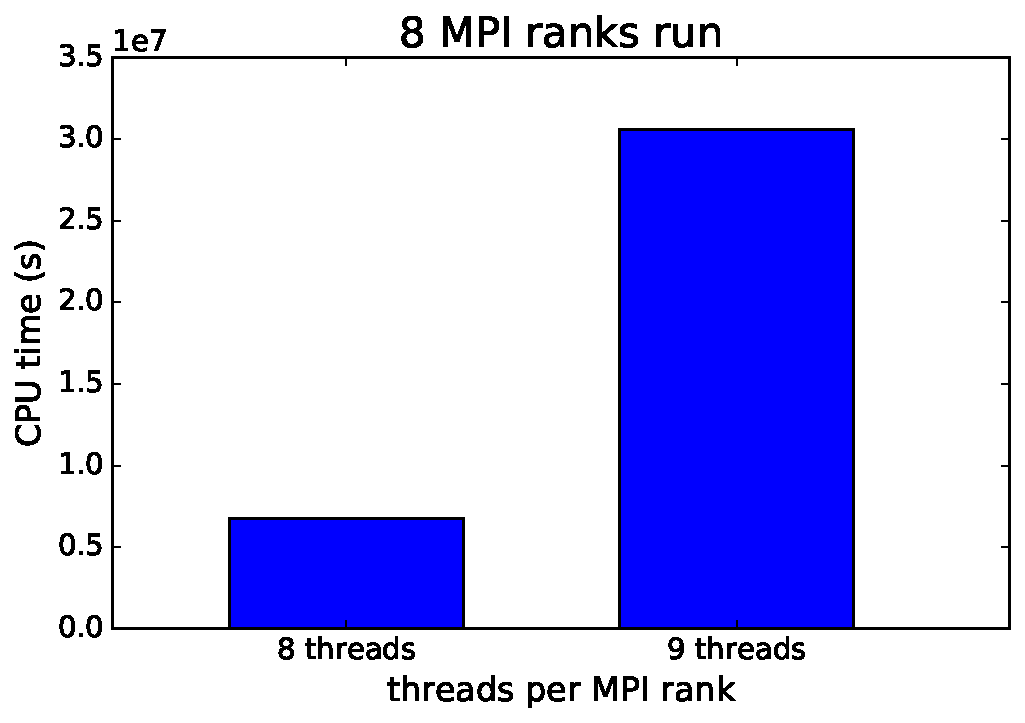
\includegraphics[width=0.5\linewidth]{threads_overload.pdf}}
	\caption{ CPU time with 8 threads per MPI rank (total of 64 threads) and 9 threads for MPI rank (total of 72 threads).}
	\label{fig:A_threadsOverload}
\end{figure}

\newpage
\section{Diagonalization cores}\label{app:ndiag}

PWscf performances in function of the total number of diagonalization cores (\texttt{-ndiag} flag).

\begin{figure}[hhh!]
	\centerline{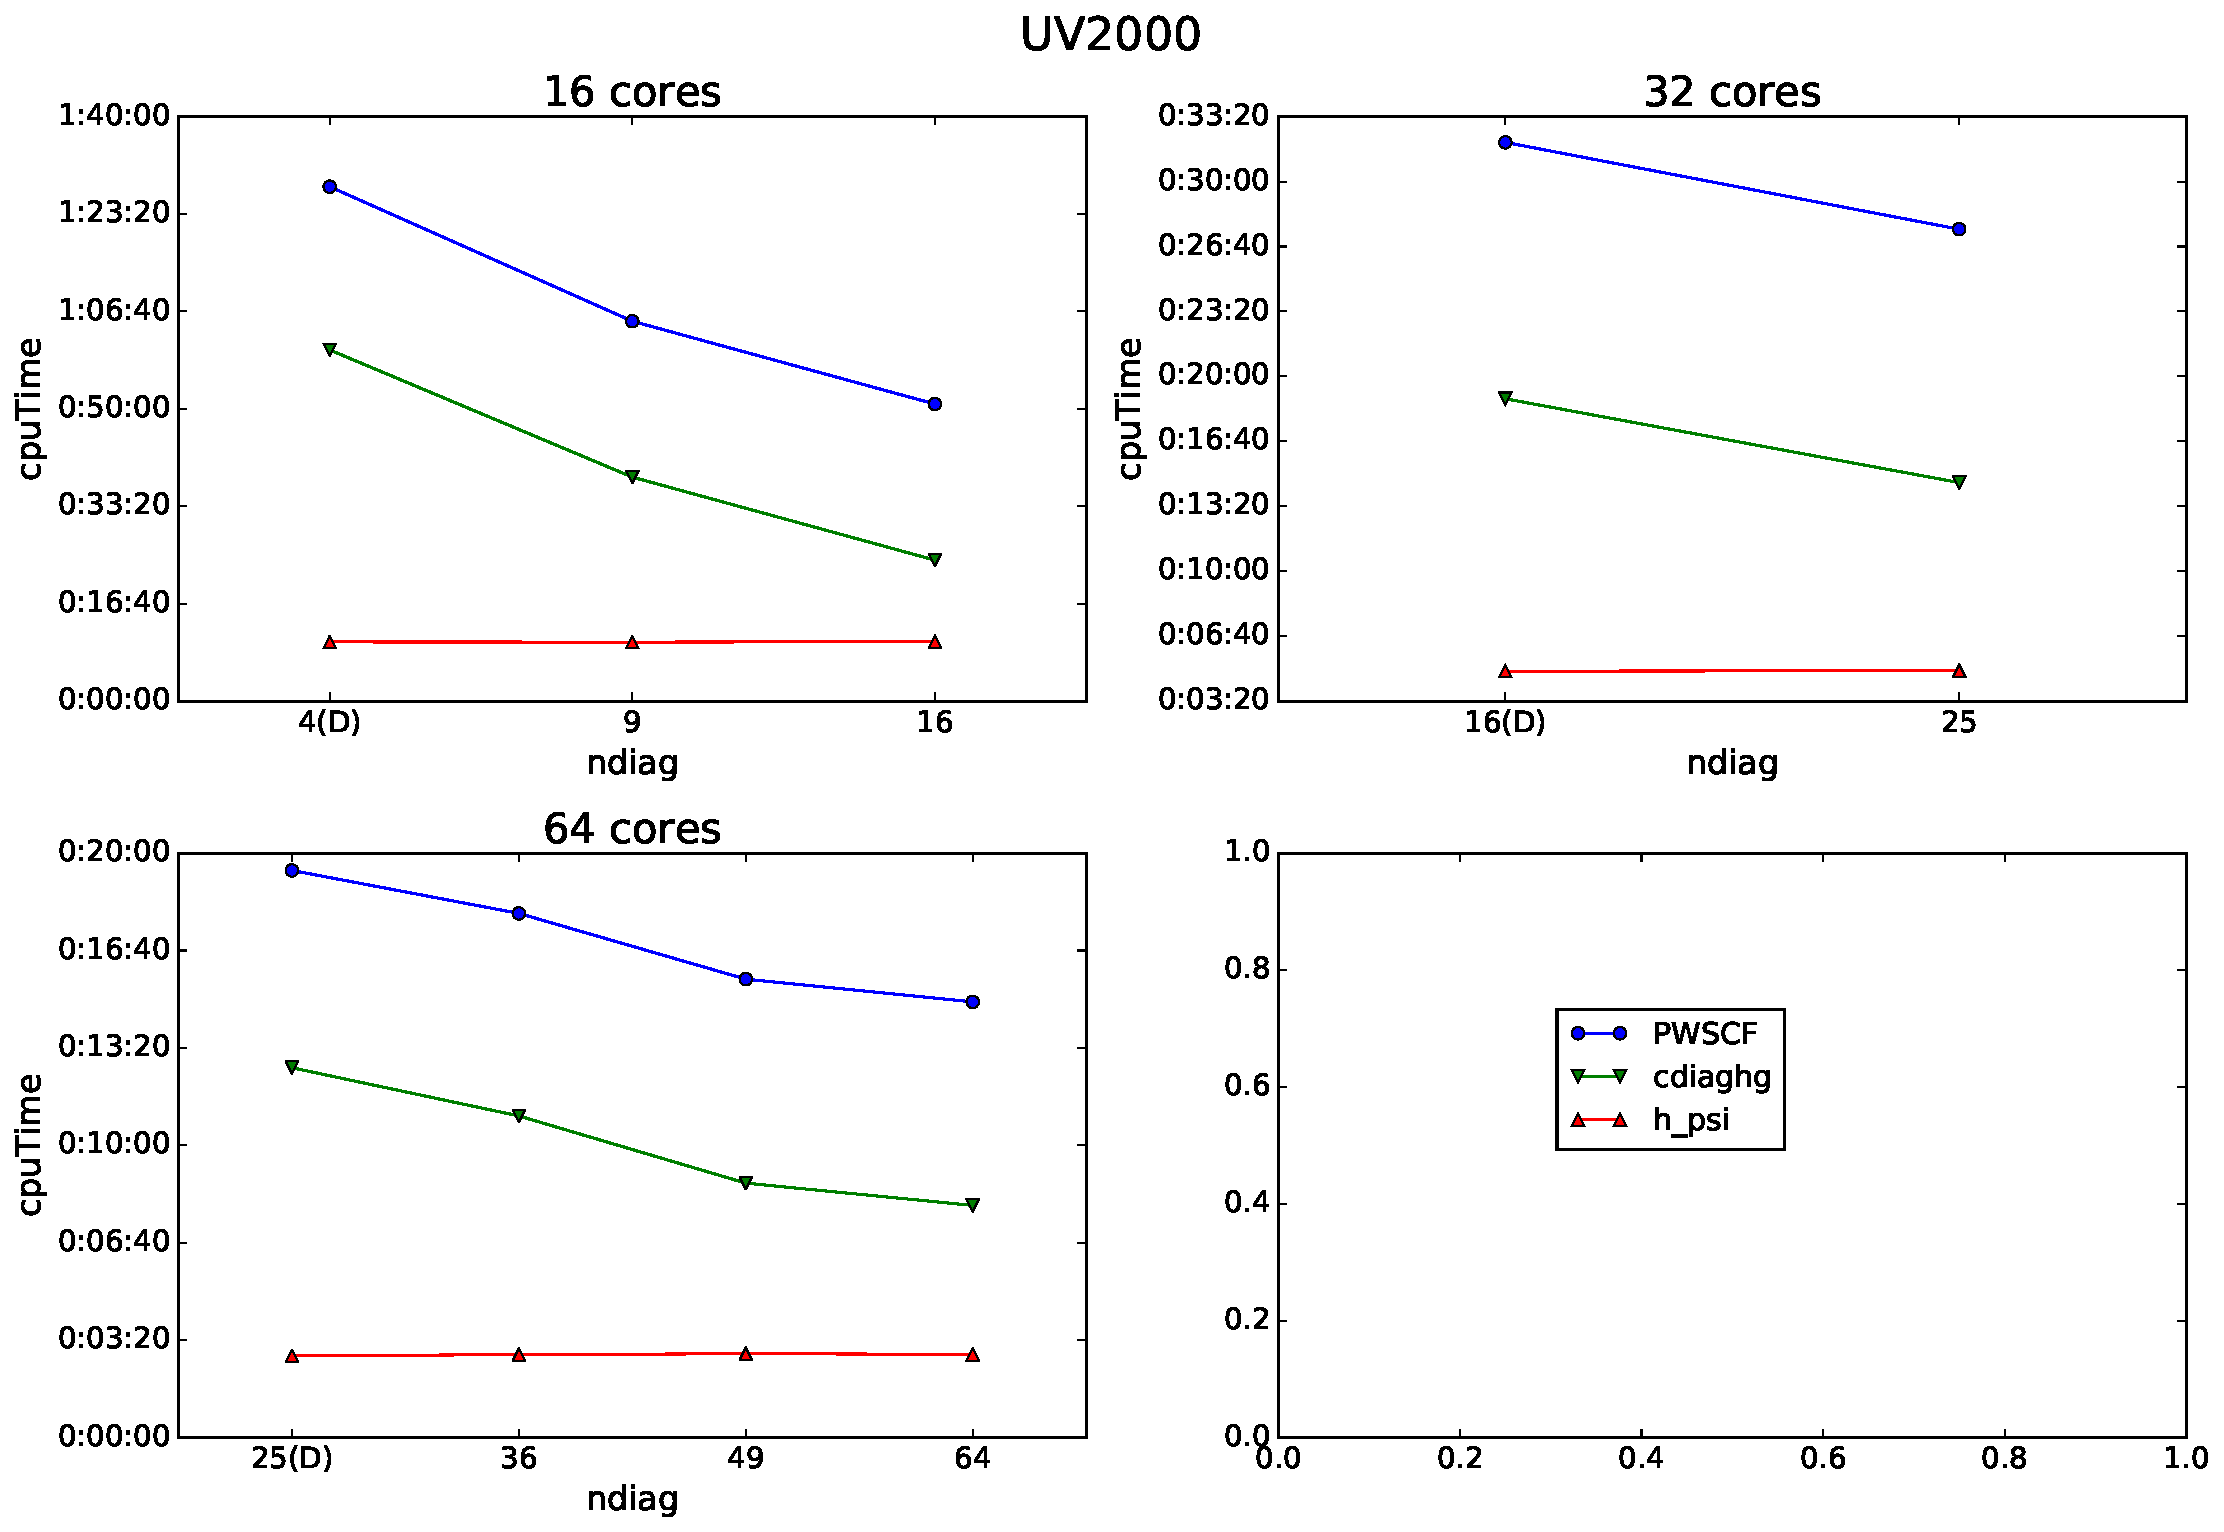
\includegraphics[width=1.2\linewidth]{sgi_ndiag.pdf}}
	\caption{``D" marks the default choice.
	}
	\label{fig:ndiagSgi}

\end{figure}
\newpage
\begin{figure}[hhh!]
	\centerline{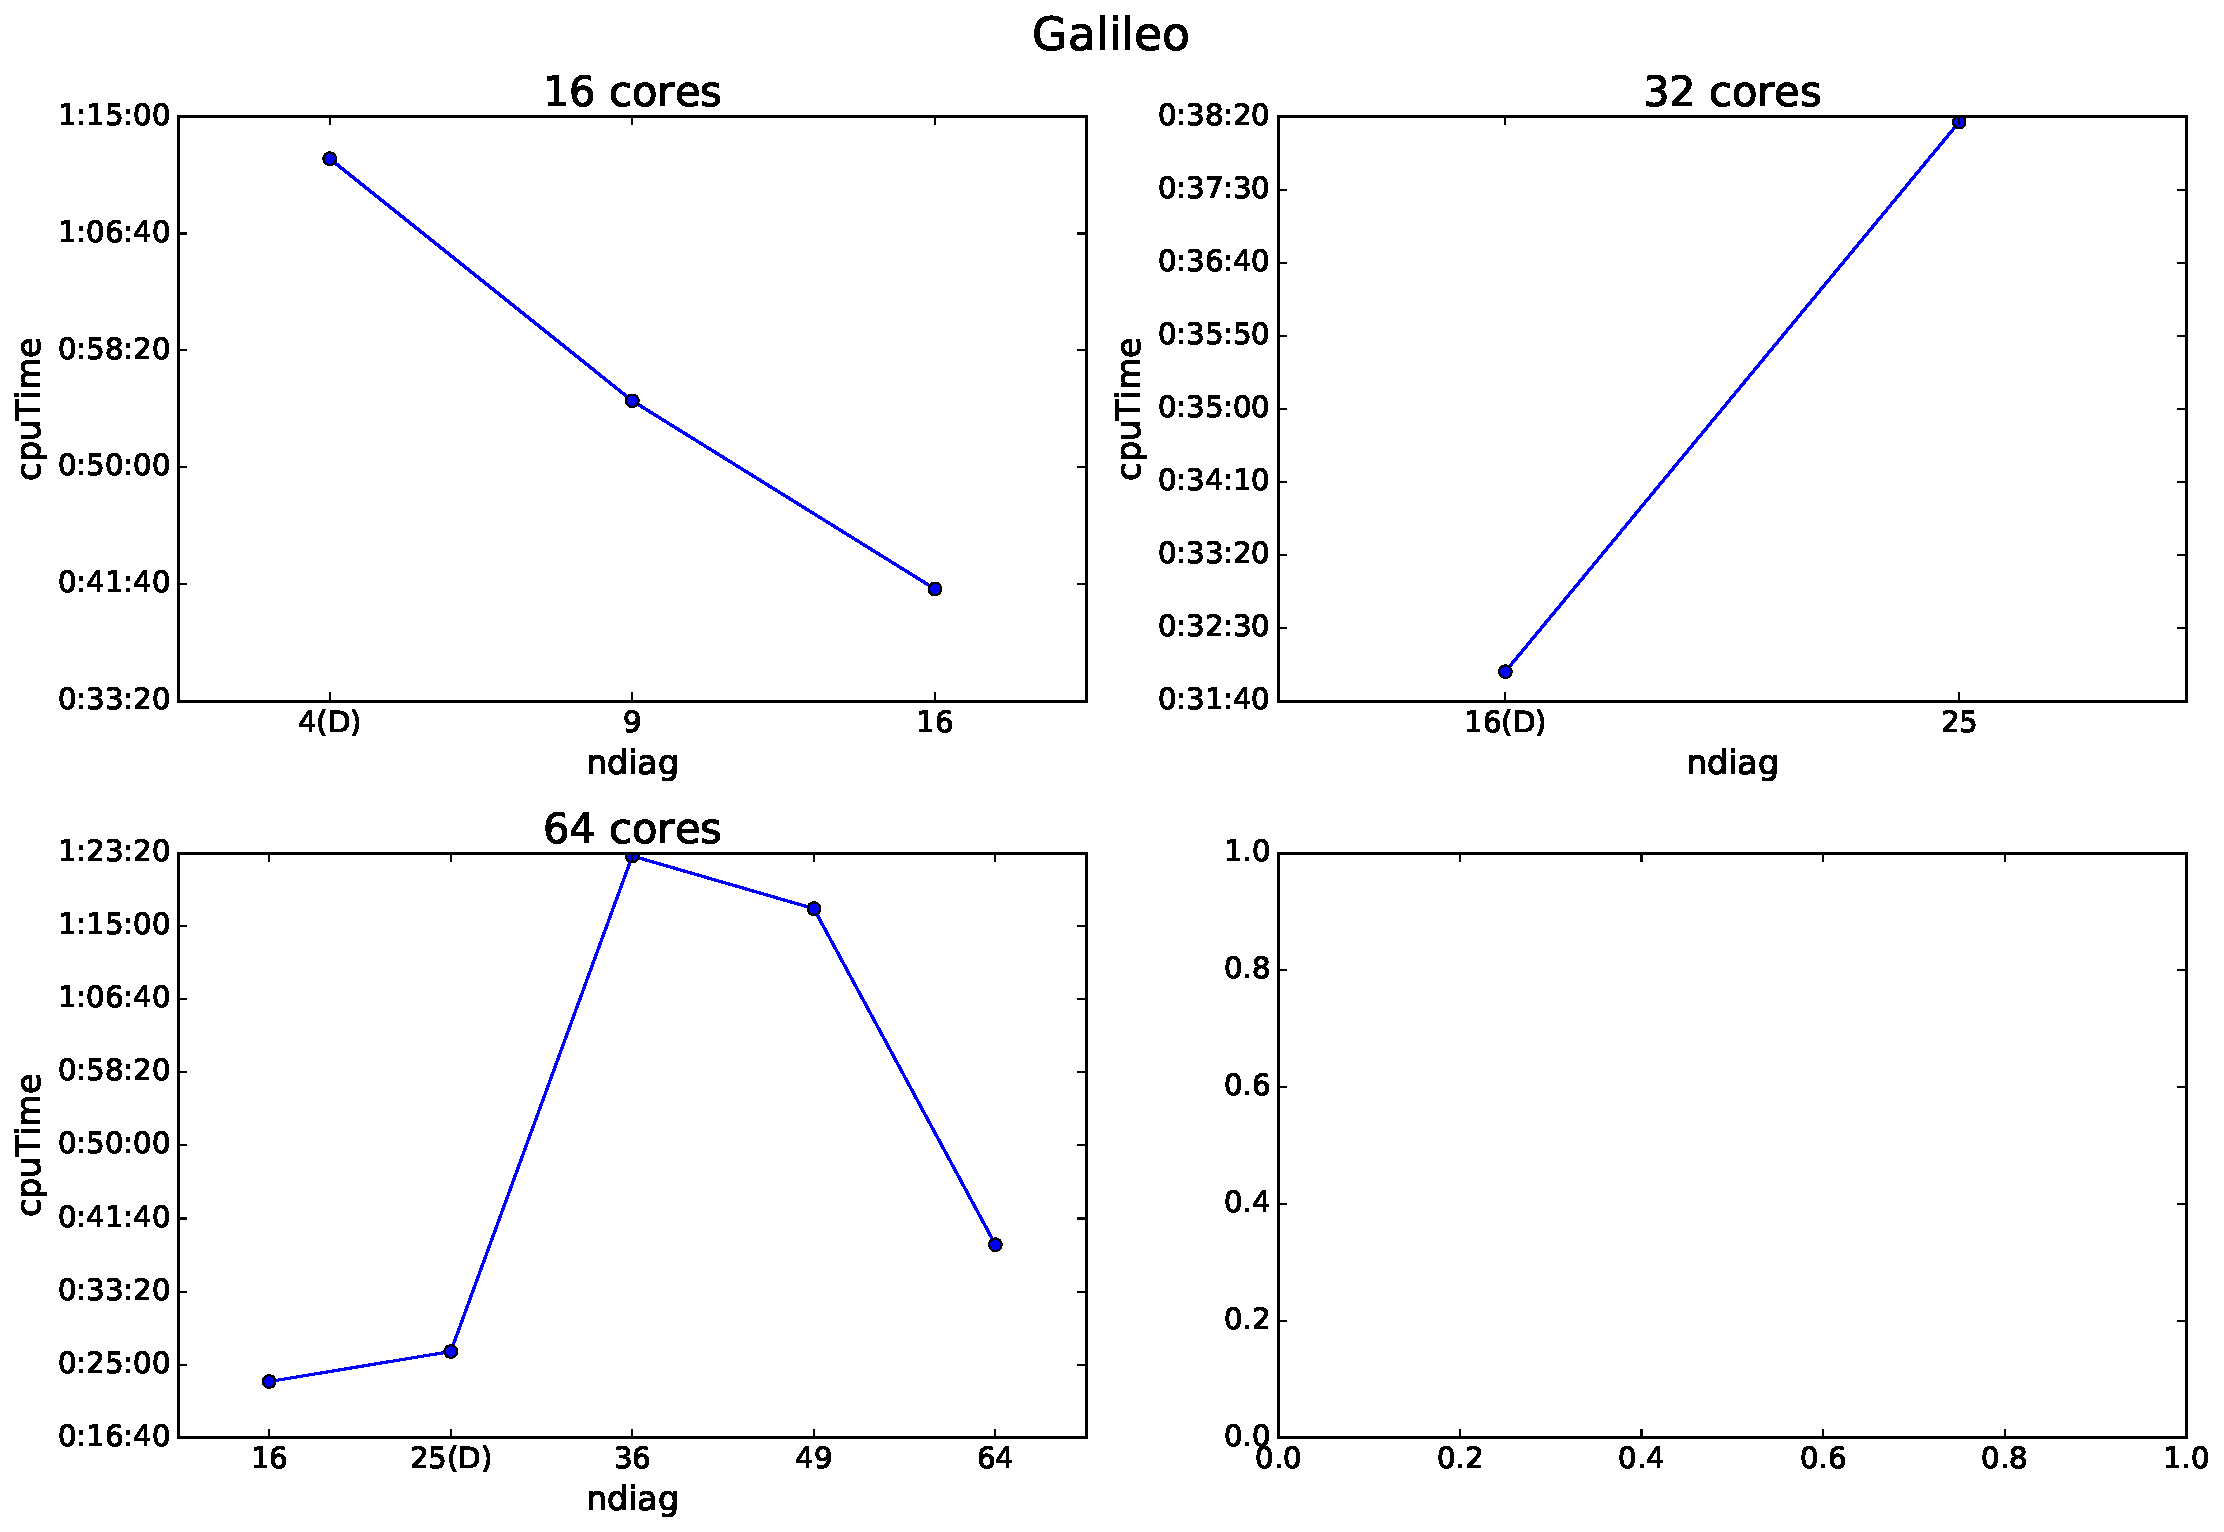
\includegraphics[width=1.2\linewidth]{cineca_ndiag.pdf}}
	\caption{ ``D" marks the default choice.
	}
	\label{fig:ndiagCineca}

\end{figure}

\newpage
\section{Resource reservation on Galileo}\label{app:PBS}
To fully reserve a single node on the cluster one must use the following PBS \texttt{qsub} directive :
\begin{verbatim}
	PBS -l select=1:ncpus=16:mpiprocs=16:mem=20gb
\end{verbatim}

Where the first number after the \texttt{select} statement is the number of nodes, \texttt{ncpus} is the number of CPUs to reserve, \texttt{mpiprocs} is the maximum number of MPI processes to be spawned and \texttt{mem} is the maximum memory required by the computation (on the single node).

Finally, to occupy only a subset of cores and leave the others unused one must specify the total number of ranks to the MPI launcher :
\begin{verbatim}
	mpirun -np 1 pw.x
\end{verbatim}
where \texttt{-np 1} sets the number of mpi processes to use and \texttt{pw.x} is the executable.
Note that in case threads are used, both explicitly or using the \texttt{OMP\_NUM\_THREADS} environment variable, the real number of CPUs used will be $N_{MPI ranks} \cdot N_{OMP threads}$.

For example: to launch a 4 core run reserving the whole 16-core node the following submission script can be used:
\begin{verbatim}
#Other PBS directives
#...
#PBS -l select=1:ncpus=16:mpiprocs=16:mem=20gb
mpirun -np 4 pw.x -i input_file -o output_file 
\end{verbatim}

\newpage 

\section{PWscf input files}\label{app:inputFiles}
\subsection{Titania}\label{app:titania}
\lstinputlisting[basicstyle=\tiny ,breaklines=true,tabsize=2]{media/listings/titania2.in}

\subsection{\CO}\label{app:Co3}
\lstinputlisting[basicstyle=\tiny ,breaklines=true,tabsize=2]{media/listings/Co3.in}

\subsection{AUSURF112}\label{app:Ausurf112}
\lstinputlisting[basicstyle=\tiny ,breaklines=true,tabsize=2]{media/listings/ausurf.in}

\subsection{OLED}\label{app:Oled}
\lstinputlisting[basicstyle=\tiny ,breaklines=true,tabsize=2]{media/listings/CBP-relax.in}


\end{appendices}


\newpage

\listoffigures


\newpage




%
% RINGRAZIAMENTI
%
% Non ti dimenticare
% Jurg Burger
% Stefano Gallucci
% 
%




%------------------------------------------------------------------
%  BIBLIOGRAPHY
%------------------------------------------------------------------
\clearpage

\addcontentsline{toc}{section}{Bibliography}
\begin{thebibliography}{9}

%------------------------------------------------------------------
%  LIBRI
%------------------------------------------------------------------

\bibitem{Atkins}
P. W. Atkins and R. S. Friedman,
Molecular Quantum Mechanics,
Oxford University Press, New York,
3rd Edition,
1997.

\bibitem{Attila}
A. Szabo, N. S. Ostlund,
Modern Quantum Chemistry: Introduction to Advanced Electronic Structure Theory,
Dover Pubblications, New York,
1996.

\bibitem{Dan}
D. Dan, Notes on General Chemistry,
Chapter 3.5, Many-electron atoms: Fermi holes and Fermi heaps,
W. H. Freeman Publisher,
2006.

\bibitem{Sakurai}
J. J. Sakurai,
Modern Quantum Mechanics,
Addison-Wesley,
Revised Edition,
1994.


\bibitem{Parr}
R. G. Parr, W. Yang,
Density Functional Theory of Atoms and Molecules,
Oxford University Press,
1989.

\bibitem{Basdevant}
J. L. Basdevant, J. Dalibard,
Quantum Mechanics,
Springer,
2005.

\bibitem{Tanenbaum}
A. S. Tanenbaum, T. Austin,
Structured Computer Organization,
Sixth edition,
Pearson,
2012

\bibitem{Martin}
R. Martin, 
Electronic Structure,
Cambridge University Press,
2008.

\bibitem{Manini}
N. Manini, 
Introduction to the Physics of Matter,
Springer,
2014.


\bibitem{Marx}
D. Marx, J. Hutter,
Ab initio Molecular Dynamics,
Basic Theory and Advanced Methods,
Cambridge University Press,
2009.

%------------------------------------------------------------------
%  PAPERS
%------------------------------------------------------------------

\bibitem{Thomas27}
L. H. Thomas, ``The calculation of atomic fields", Proc. Cambridge Phil. Soc. \textbf{23},542 (1927)

\bibitem{Fermi27}
E. Fermi,``Un Metodo Statistico per la Determinazione di alcune Priopriet\'a dell'Atomo", Rend. Lincei \textbf{6}, 602 (1927)

\bibitem{HK}
P. Hohenberg and W. Kohn, ``Inhomogeneous Electron Gas",  Physical Review \textbf{136} (3B): B864 (1964)

\bibitem{KS}
W. Kohn and L. J. Sham, ``Self-Consistent Equations Including Exchange and Correlation Effects". Physical Review \textbf{140} (4A): A1133 (1965)

\bibitem{QE}
P. Giannozzi , S. Baroni , N. Bonini,``QUANTUM ESPRESSO: a modular and open-source software project for quantum simulations of materials", J. Phys.: Condens. Matter \textbf{21} (2009) 395502 (19pp)

\bibitem{Davidson}
E. R. Davidson, ``Super-Matrix Methods", Comput. Phys. Comm., \textbf{53} 49 (1989)

\bibitem{Johnson}
D. D. Johnson, ``Modified Broyden’s method for accelerating convergence in self-consistent calculations", Phys. Rev. B \textbf{38}, 12807 (1988)


\bibitem{QE2}
P. Giannozzi, C. Cavazzoni,
``Large-scale computing with \QE",
Il Nuovo Cimento, Vol. \textbf{32 C}, N. 2, (2009).



\bibitem{FFTPAPER}
D. Stankovi, P. Jovanovi, A. Jovi, V. Slavni, D. Vudragovi, A. Bala,
``High-Performance Computing Infrastructure for South East Europe's Research Communities: Results of the HP-SEE User Forum 2012",
Springer,
2014.

\bibitem{prace}
I. Girotto, N. Varini, F. Spiga, C. Cavazzoni, D. Ceresoli, L. Martin-Samos, T. Gorni,
``Enabling of Quantum ESPRESSO to Petascale Scientific Challenges",
PRACE Whitepapers,
PRACE,
2012.

\bibitem{Cannon}
L. E. Cannon, 
``A Cellular Computer to Implement the Kalman Filter Algorithm",
Montana State University,
1969.

\bibitem{Titania1}
C. Marchiori, G. Di Liberto, G. Soliveri, L. Loconte, L. Lo Presti, D. Meroni, M. Ceotto, C. Oliva, S. Cappelli, G. Cappelletti, C. Aieta, S. Ardizzone,
``Unraveling the Cooperative Mechanism of Visible-Light Absorption in Bulk N,Nb Codoped TiO\textsubscript{2} Powders of Nanomaterials",
The Journal of Physical Chemistry C \textbf{118} 41, (2014).

\bibitem{Titania2}
U. Diebold,
``The surface science of titanium dioxide",
Surf. Sci. Rep. \textbf{48} 53-229, (2003) .

\bibitem{Titania3}
O. Carp, 
``Photoinduced Reactivity of Titanium Dioxide", 
Prog. Solid State Chem. \textbf{32}, 33−177, (2004).

\bibitem{Titania4}
X. Chen, S. Mao, 
``Titanium Dioxide Nanomaterials: Synthesis, Properties, Modifications, and Applications", 
Chem. Rev. \textbf{107}, 2891−2959 (2007).

\bibitem{Titania5}
A. Fujishima, X. Zhang,D. Tryk, 
``Tio2 Photocatalysis and Related Surface Phenomena", 
Surf. Sci. Rep. \textbf{63}, 515−582 (2008).


%------------------------------------------------------------------
%  URL
%------------------------------------------------------------------
\bibitem{Carati}
A. Carati, L.Galgani,
Appunti di Meccanica Razionale 1,
\url{http://users.mat.unimi.it/users/carati/#Didattica}.


\bibitem{QEManual}
``User's Guide for Quantum ESPRESSO", \url{http://www.quantum-espresso.org/wp-content/uploads/Doc/user_guide.pdf}.

\bibitem{MPI}
``MPI :A Message-Passing Interface Standard", \url{http://www.mpi-forum.org/docs/mpi-3.1/mpi31-report.pdf}

\bibitem{OMP}
``OpenMP Application Programming Interface", \url{http://www.openmp.org/mp-documents/openmp-4.5.pdf}

\bibitem{BLAS}
BLAS, ``Basic Linear Algebra Subprograms", \url{http://www.netlib.org/blas/}.

\bibitem{LAPACK}
LAPACK, ``Linear Algebra PACKage", \url{http://www.netlib.org/lapack/}

\bibitem{SCALAPACK}
ScaLAPACK, ``Scalable Linear Algebra PACKage", \url{http://www.netlib.org/scalapack/}

\bibitem{FFTW}
``Fast Fourier Transform in the West", \url{http://www.fftw.org/}.

\bibitem{Galileo}
CINECA's Galileo multicomputer cluster,
\url{http://www.top500.org/system/178549},
\url{http://www.hpc.cineca.it/hardware/galileo}.


\bibitem{MPT}
Full specification of the Message Passing Toolkit can be retrieved using the command : \texttt{man mpt}.

\bibitem{VH}
VH-HPS, 
Virtual Institute – High Productivity Supercomputing, 
\url{http://www.vi-hps.org}.

\bibitem{SCOREPManual}
\texttt{scorep} user manual, 
v1.4.2,
\url{https://silc.zih.tu-dresden.de/scorep-current/pdf/scorep.pdf}.

\bibitem{qetools}
qetools, ``tools to profile Quantum Espresso PWscf package", Giorgio Ruffa, \url{https://github.com/xmooner/qetools}.

\bibitem{PWinput}
PWscf input documentation, \url{http://www.quantum-espresso.org/wp-content/uploads/Doc/INPUT_PW.html}.

\bibitem{Condor}
Condor project homepage, \url{https://research.cs.wisc.edu/htcondor/}

\bibitem{HPC}
HPC Advisory council,
``Quantum ESPRESSO Performance Benchmark and Profiling",
\url{http://www.hpcadvisorycouncil.com/}.



\end{thebibliography}


\end{document}


